\documentclass[twoside]{book}

% Packages required by doxygen
\usepackage{fixltx2e}
\usepackage{calc}
\usepackage{doxygen}
\usepackage[export]{adjustbox} % also loads graphicx
\usepackage{graphicx}
\usepackage[utf8]{inputenc}
\usepackage{makeidx}
\usepackage{multicol}
\usepackage{multirow}
\PassOptionsToPackage{warn}{textcomp}
\usepackage{textcomp}
\usepackage[nointegrals]{wasysym}
\usepackage[table]{xcolor}

% Font selection
\usepackage[T1]{fontenc}
\usepackage[scaled=.90]{helvet}
\usepackage{courier}
\usepackage{amssymb}
\usepackage{sectsty}
\renewcommand{\familydefault}{\sfdefault}
\allsectionsfont{%
  \fontseries{bc}\selectfont%
  \color{darkgray}%
}
\renewcommand{\DoxyLabelFont}{%
  \fontseries{bc}\selectfont%
  \color{darkgray}%
}
\newcommand{\+}{\discretionary{\mbox{\scriptsize$\hookleftarrow$}}{}{}}

% Page & text layout
\usepackage{geometry}
\geometry{%
  a4paper,%
  top=2.5cm,%
  bottom=2.5cm,%
  left=2.5cm,%
  right=2.5cm%
}
\tolerance=750
\hfuzz=15pt
\hbadness=750
\setlength{\emergencystretch}{15pt}
\setlength{\parindent}{0cm}
\setlength{\parskip}{3ex plus 2ex minus 2ex}
\makeatletter
\renewcommand{\paragraph}{%
  \@startsection{paragraph}{4}{0ex}{-1.0ex}{1.0ex}{%
    \normalfont\normalsize\bfseries\SS@parafont%
  }%
}
\renewcommand{\subparagraph}{%
  \@startsection{subparagraph}{5}{0ex}{-1.0ex}{1.0ex}{%
    \normalfont\normalsize\bfseries\SS@subparafont%
  }%
}
\makeatother

% Headers & footers
\usepackage{fancyhdr}
\pagestyle{fancyplain}
\fancyhead[LE]{\fancyplain{}{\bfseries\thepage}}
\fancyhead[CE]{\fancyplain{}{}}
\fancyhead[RE]{\fancyplain{}{\bfseries\leftmark}}
\fancyhead[LO]{\fancyplain{}{\bfseries\rightmark}}
\fancyhead[CO]{\fancyplain{}{}}
\fancyhead[RO]{\fancyplain{}{\bfseries\thepage}}
\fancyfoot[LE]{\fancyplain{}{}}
\fancyfoot[CE]{\fancyplain{}{}}
\fancyfoot[RE]{\fancyplain{}{\bfseries\scriptsize Generated by Doxygen }}
\fancyfoot[LO]{\fancyplain{}{\bfseries\scriptsize Generated by Doxygen }}
\fancyfoot[CO]{\fancyplain{}{}}
\fancyfoot[RO]{\fancyplain{}{}}
\renewcommand{\footrulewidth}{0.4pt}
\renewcommand{\chaptermark}[1]{%
  \markboth{#1}{}%
}
\renewcommand{\sectionmark}[1]{%
  \markright{\thesection\ #1}%
}

% Indices & bibliography
\usepackage{natbib}
\usepackage[titles]{tocloft}
\setcounter{tocdepth}{3}
\setcounter{secnumdepth}{5}
\makeindex

% Hyperlinks (required, but should be loaded last)
\usepackage{ifpdf}
\ifpdf
  \usepackage[pdftex,pagebackref=true]{hyperref}
\else
  \usepackage[ps2pdf,pagebackref=true]{hyperref}
\fi
\hypersetup{%
  colorlinks=true,%
  linkcolor=blue,%
  citecolor=blue,%
  unicode%
}

% Custom commands
\newcommand{\clearemptydoublepage}{%
  \newpage{\pagestyle{empty}\cleardoublepage}%
}

\usepackage{caption}
\captionsetup{labelsep=space,justification=centering,font={bf},singlelinecheck=off,skip=4pt,position=top}

%===== C O N T E N T S =====

\begin{document}

% Titlepage & ToC
\hypersetup{pageanchor=false,
             bookmarksnumbered=true,
             pdfencoding=unicode
            }
\pagenumbering{alph}
\begin{titlepage}
\vspace*{7cm}
\begin{center}%
{\Large My Project }\\
\vspace*{1cm}
{\large Generated by Doxygen 1.8.14}\\
\end{center}
\end{titlepage}
\clearemptydoublepage
\pagenumbering{roman}
\tableofcontents
\clearemptydoublepage
\pagenumbering{arabic}
\hypersetup{pageanchor=true}

%--- Begin generated contents ---
\chapter{Namespace Index}
\section{Packages}
Here are the packages with brief descriptions (if available)\+:\begin{DoxyCompactList}
\item\contentsline{section}{\mbox{\hyperlink{namespace_class_library_server}{Class\+Library\+Server}} }{\pageref{namespace_class_library_server}}{}
\item\contentsline{section}{\mbox{\hyperlink{namespace_class_library_server_1_1_struct}{Class\+Library\+Server.\+Struct}} }{\pageref{namespace_class_library_server_1_1_struct}}{}
\item\contentsline{section}{\mbox{\hyperlink{namespace_console_app_server}{Console\+App\+Server}} }{\pageref{namespace_console_app_server}}{}
\item\contentsline{section}{\mbox{\hyperlink{namespace_objects}{Objects}} }{\pageref{namespace_objects}}{}
\item\contentsline{section}{\mbox{\hyperlink{namespace_p_e_d_scanner}{P\+E\+D\+Scanner}} }{\pageref{namespace_p_e_d_scanner}}{}
\item\contentsline{section}{\mbox{\hyperlink{namespace_p_e_d_scanner_1_1_properties}{P\+E\+D\+Scanner.\+Properties}} }{\pageref{namespace_p_e_d_scanner_1_1_properties}}{}
\item\contentsline{section}{\mbox{\hyperlink{namespace_p_e_d_scanner_console_app}{P\+E\+D\+Scanner\+Console\+App}} }{\pageref{namespace_p_e_d_scanner_console_app}}{}
\item\contentsline{section}{\mbox{\hyperlink{namespace_p_e_d_scanner_lib}{P\+E\+D\+Scanner\+Lib}} }{\pageref{namespace_p_e_d_scanner_lib}}{}
\item\contentsline{section}{\mbox{\hyperlink{namespace_p_e_d_scanner_lib_1_1_core}{P\+E\+D\+Scanner\+Lib.\+Core}} }{\pageref{namespace_p_e_d_scanner_lib_1_1_core}}{}
\item\contentsline{section}{\mbox{\hyperlink{namespace_p_e_d_scanner_lib_1_1_objects}{P\+E\+D\+Scanner\+Lib.\+Objects}} }{\pageref{namespace_p_e_d_scanner_lib_1_1_objects}}{}
\item\contentsline{section}{\mbox{\hyperlink{namespace_p_e_d_scanner_lib_1_1_struct}{P\+E\+D\+Scanner\+Lib.\+Struct}} }{\pageref{namespace_p_e_d_scanner_lib_1_1_struct}}{}
\item\contentsline{section}{\mbox{\hyperlink{namespace_p_e_scanner}{P\+E\+Scanner}} }{\pageref{namespace_p_e_scanner}}{}
\item\contentsline{section}{\mbox{\hyperlink{namespace_server64}{Server64}} }{\pageref{namespace_server64}}{}
\item\contentsline{section}{\mbox{\hyperlink{namespace_service64_proxy}{Service64\+Proxy}} }{\pageref{namespace_service64_proxy}}{}
\item\contentsline{section}{\mbox{\hyperlink{namespace_wizard}{Wizard}} }{\pageref{namespace_wizard}}{}
\end{DoxyCompactList}

\chapter{Hierarchical Index}
\section{Class Hierarchy}
This inheritance list is sorted roughly, but not completely, alphabetically\+:\begin{DoxyCompactList}
\item Application\begin{DoxyCompactList}
\item \contentsline{section}{Wizard.\+App}{\pageref{class_wizard_1_1_app}}{}
\end{DoxyCompactList}
\item Client\+Base\begin{DoxyCompactList}
\item \contentsline{section}{Service64\+Proxy.\+Service64}{\pageref{class_service64_proxy_1_1_service64}}{}
\end{DoxyCompactList}
\item \contentsline{section}{P\+E\+D\+Scanner\+Lib.\+Objects.\+Dependecies\+Object}{\pageref{class_p_e_d_scanner_lib_1_1_objects_1_1_dependecies_object}}{}
\item \contentsline{section}{P\+E\+D\+Scanner\+Lib.\+Objects.\+Directory\+Object}{\pageref{class_p_e_d_scanner_lib_1_1_objects_1_1_directory_object}}{}
\item \contentsline{section}{P\+E\+D\+Scanner\+Lib.\+Objects.\+Error\+Object}{\pageref{class_p_e_d_scanner_lib_1_1_objects_1_1_error_object}}{}
\item \contentsline{section}{Objects.\+Export\+Object}{\pageref{class_objects_1_1_export_object}}{}
\item Form\begin{DoxyCompactList}
\item \contentsline{section}{P\+E\+Scanner.\+Main\+Window}{\pageref{class_p_e_scanner_1_1_main_window}}{}
\end{DoxyCompactList}
\item \contentsline{section}{Objects.\+Function\+Object}{\pageref{class_objects_1_1_function_object}}{}
\begin{DoxyCompactList}
\item \contentsline{section}{Objects.\+Import\+Function\+Object}{\pageref{class_objects_1_1_import_function_object}}{}
\item \contentsline{section}{Objects.\+Import\+Function\+Object}{\pageref{class_objects_1_1_import_function_object}}{}
\end{DoxyCompactList}
\item \contentsline{section}{P\+E\+D\+Scanner\+Lib.\+Objects.\+Header\+Object}{\pageref{class_p_e_d_scanner_lib_1_1_objects_1_1_header_object}}{}
\item \contentsline{section}{Class\+Library\+Server.\+Struct.\+Pe\+Header\+Reader.\+I\+M\+A\+G\+E\+\_\+\+D\+A\+T\+A\+\_\+\+D\+I\+R\+E\+C\+T\+O\+RY}{\pageref{struct_class_library_server_1_1_struct_1_1_pe_header_reader_1_1_i_m_a_g_e___d_a_t_a___d_i_r_e_c_t_o_r_y}}{}
\item \contentsline{section}{P\+E\+D\+Scanner\+Lib.\+Struct.\+Pe\+Header\+Reader.\+I\+M\+A\+G\+E\+\_\+\+D\+A\+T\+A\+\_\+\+D\+I\+R\+E\+C\+T\+O\+RY}{\pageref{struct_p_e_d_scanner_lib_1_1_struct_1_1_pe_header_reader_1_1_i_m_a_g_e___d_a_t_a___d_i_r_e_c_t_o_r_y}}{}
\item \contentsline{section}{P\+E\+D\+Scanner\+Lib.\+Struct.\+Pe\+Header\+Reader.\+I\+M\+A\+G\+E\+\_\+\+D\+O\+S\+\_\+\+H\+E\+A\+D\+ER}{\pageref{struct_p_e_d_scanner_lib_1_1_struct_1_1_pe_header_reader_1_1_i_m_a_g_e___d_o_s___h_e_a_d_e_r}}{}
\item \contentsline{section}{Class\+Library\+Server.\+Struct.\+Pe\+Header\+Reader.\+I\+M\+A\+G\+E\+\_\+\+D\+O\+S\+\_\+\+H\+E\+A\+D\+ER}{\pageref{struct_class_library_server_1_1_struct_1_1_pe_header_reader_1_1_i_m_a_g_e___d_o_s___h_e_a_d_e_r}}{}
\item \contentsline{section}{P\+E\+D\+Scanner\+Lib.\+Struct.\+I\+M\+A\+G\+E\+\_\+\+E\+X\+P\+O\+R\+T\+\_\+\+D\+I\+R\+E\+C\+T\+O\+RY}{\pageref{struct_p_e_d_scanner_lib_1_1_struct_1_1_i_m_a_g_e___e_x_p_o_r_t___d_i_r_e_c_t_o_r_y}}{}
\item \contentsline{section}{Class\+Library\+Server.\+Struct.\+I\+M\+A\+G\+E\+\_\+\+E\+X\+P\+O\+R\+T\+\_\+\+D\+I\+R\+E\+C\+T\+O\+RY}{\pageref{struct_class_library_server_1_1_struct_1_1_i_m_a_g_e___e_x_p_o_r_t___d_i_r_e_c_t_o_r_y}}{}
\item \contentsline{section}{P\+E\+D\+Scanner\+Lib.\+Struct.\+I\+M\+A\+G\+E\+\_\+\+F\+I\+L\+E\+\_\+\+H\+E\+A\+D\+ER}{\pageref{struct_p_e_d_scanner_lib_1_1_struct_1_1_i_m_a_g_e___f_i_l_e___h_e_a_d_e_r}}{}
\item \contentsline{section}{Class\+Library\+Server.\+Struct.\+I\+M\+A\+G\+E\+\_\+\+F\+I\+L\+E\+\_\+\+H\+E\+A\+D\+ER}{\pageref{struct_class_library_server_1_1_struct_1_1_i_m_a_g_e___f_i_l_e___h_e_a_d_e_r}}{}
\item \contentsline{section}{P\+E\+D\+Scanner\+Lib.\+Struct.\+Pe\+Header\+Reader.\+I\+M\+A\+G\+E\+\_\+\+I\+M\+P\+O\+R\+T\+\_\+\+B\+Y\+\_\+\+N\+A\+ME}{\pageref{struct_p_e_d_scanner_lib_1_1_struct_1_1_pe_header_reader_1_1_i_m_a_g_e___i_m_p_o_r_t___b_y___n_a_m_e}}{}
\item \contentsline{section}{Class\+Library\+Server.\+Struct.\+Pe\+Header\+Reader.\+I\+M\+A\+G\+E\+\_\+\+I\+M\+P\+O\+R\+T\+\_\+\+B\+Y\+\_\+\+N\+A\+ME}{\pageref{struct_class_library_server_1_1_struct_1_1_pe_header_reader_1_1_i_m_a_g_e___i_m_p_o_r_t___b_y___n_a_m_e}}{}
\item \contentsline{section}{P\+E\+D\+Scanner\+Lib.\+Struct.\+I\+M\+A\+G\+E\+\_\+\+I\+M\+P\+O\+R\+T\+\_\+\+B\+Y\+\_\+\+N\+A\+ME}{\pageref{struct_p_e_d_scanner_lib_1_1_struct_1_1_i_m_a_g_e___i_m_p_o_r_t___b_y___n_a_m_e}}{}
\item \contentsline{section}{Class\+Library\+Server.\+Struct.\+I\+M\+A\+G\+E\+\_\+\+I\+M\+P\+O\+R\+T\+\_\+\+B\+Y\+\_\+\+N\+A\+ME}{\pageref{struct_class_library_server_1_1_struct_1_1_i_m_a_g_e___i_m_p_o_r_t___b_y___n_a_m_e}}{}
\item \contentsline{section}{Class\+Library\+Server.\+Struct.\+I\+M\+A\+G\+E\+\_\+\+I\+M\+P\+O\+R\+T\+\_\+\+B\+Y\+\_\+\+N\+A\+M\+E64}{\pageref{struct_class_library_server_1_1_struct_1_1_i_m_a_g_e___i_m_p_o_r_t___b_y___n_a_m_e64}}{}
\item \contentsline{section}{Class\+Library\+Server.\+Struct.\+Pe\+Header\+Reader.\+I\+M\+A\+G\+E\+\_\+\+I\+M\+P\+O\+R\+T\+\_\+\+D\+E\+S\+C\+R\+I\+P\+T\+OR}{\pageref{struct_class_library_server_1_1_struct_1_1_pe_header_reader_1_1_i_m_a_g_e___i_m_p_o_r_t___d_e_s_c_r_i_p_t_o_r}}{}
\item \contentsline{section}{P\+E\+D\+Scanner\+Lib.\+Struct.\+Pe\+Header\+Reader.\+I\+M\+A\+G\+E\+\_\+\+I\+M\+P\+O\+R\+T\+\_\+\+D\+E\+S\+C\+R\+I\+P\+T\+OR}{\pageref{struct_p_e_d_scanner_lib_1_1_struct_1_1_pe_header_reader_1_1_i_m_a_g_e___i_m_p_o_r_t___d_e_s_c_r_i_p_t_o_r}}{}
\item \contentsline{section}{P\+E\+D\+Scanner\+Lib.\+Struct.\+I\+M\+A\+G\+E\+\_\+\+I\+M\+P\+O\+R\+T\+\_\+\+D\+E\+S\+C\+R\+I\+P\+T\+OR}{\pageref{struct_p_e_d_scanner_lib_1_1_struct_1_1_i_m_a_g_e___i_m_p_o_r_t___d_e_s_c_r_i_p_t_o_r}}{}
\item \contentsline{section}{Class\+Library\+Server.\+Struct.\+I\+M\+A\+G\+E\+\_\+\+I\+M\+P\+O\+R\+T\+\_\+\+D\+E\+S\+C\+R\+I\+P\+T\+OR}{\pageref{struct_class_library_server_1_1_struct_1_1_i_m_a_g_e___i_m_p_o_r_t___d_e_s_c_r_i_p_t_o_r}}{}
\item \contentsline{section}{Class\+Library\+Server.\+Struct.\+I\+M\+A\+G\+E\+\_\+\+I\+M\+P\+O\+R\+T\+\_\+\+D\+E\+S\+C\+R\+I\+P\+T\+O\+R64}{\pageref{struct_class_library_server_1_1_struct_1_1_i_m_a_g_e___i_m_p_o_r_t___d_e_s_c_r_i_p_t_o_r64}}{}
\item \contentsline{section}{Class\+Library\+Server.\+Struct.\+Pe\+Header\+Reader.\+I\+M\+A\+G\+E\+\_\+\+O\+P\+T\+I\+O\+N\+A\+L\+\_\+\+H\+E\+A\+D\+E\+R32}{\pageref{struct_class_library_server_1_1_struct_1_1_pe_header_reader_1_1_i_m_a_g_e___o_p_t_i_o_n_a_l___h_e_a_d_e_r32}}{}
\item \contentsline{section}{P\+E\+D\+Scanner\+Lib.\+Struct.\+Pe\+Header\+Reader.\+I\+M\+A\+G\+E\+\_\+\+O\+P\+T\+I\+O\+N\+A\+L\+\_\+\+H\+E\+A\+D\+E\+R32}{\pageref{struct_p_e_d_scanner_lib_1_1_struct_1_1_pe_header_reader_1_1_i_m_a_g_e___o_p_t_i_o_n_a_l___h_e_a_d_e_r32}}{}
\item \contentsline{section}{Class\+Library\+Server.\+Struct.\+Pe\+Header\+Reader.\+I\+M\+A\+G\+E\+\_\+\+O\+P\+T\+I\+O\+N\+A\+L\+\_\+\+H\+E\+A\+D\+E\+R64}{\pageref{struct_class_library_server_1_1_struct_1_1_pe_header_reader_1_1_i_m_a_g_e___o_p_t_i_o_n_a_l___h_e_a_d_e_r64}}{}
\item \contentsline{section}{P\+E\+D\+Scanner\+Lib.\+Struct.\+Pe\+Header\+Reader.\+I\+M\+A\+G\+E\+\_\+\+O\+P\+T\+I\+O\+N\+A\+L\+\_\+\+H\+E\+A\+D\+E\+R64}{\pageref{struct_p_e_d_scanner_lib_1_1_struct_1_1_pe_header_reader_1_1_i_m_a_g_e___o_p_t_i_o_n_a_l___h_e_a_d_e_r64}}{}
\item \contentsline{section}{Class\+Library\+Server.\+Struct.\+Pe\+Header\+Reader.\+I\+M\+A\+G\+E\+\_\+\+S\+E\+C\+T\+I\+O\+N\+\_\+\+H\+E\+A\+D\+ER}{\pageref{struct_class_library_server_1_1_struct_1_1_pe_header_reader_1_1_i_m_a_g_e___s_e_c_t_i_o_n___h_e_a_d_e_r}}{}
\item \contentsline{section}{P\+E\+D\+Scanner\+Lib.\+Struct.\+Pe\+Header\+Reader.\+I\+M\+A\+G\+E\+\_\+\+S\+E\+C\+T\+I\+O\+N\+\_\+\+H\+E\+A\+D\+ER}{\pageref{struct_p_e_d_scanner_lib_1_1_struct_1_1_pe_header_reader_1_1_i_m_a_g_e___s_e_c_t_i_o_n___h_e_a_d_e_r}}{}
\item \contentsline{section}{P\+E\+D\+Scanner\+Lib.\+Struct.\+I\+M\+A\+G\+E\+\_\+\+S\+E\+C\+T\+I\+O\+N\+\_\+\+H\+E\+A\+D\+ER}{\pageref{struct_p_e_d_scanner_lib_1_1_struct_1_1_i_m_a_g_e___s_e_c_t_i_o_n___h_e_a_d_e_r}}{}
\item \contentsline{section}{Class\+Library\+Server.\+Struct.\+I\+M\+A\+G\+E\+\_\+\+S\+E\+C\+T\+I\+O\+N\+\_\+\+H\+E\+A\+D\+ER}{\pageref{struct_class_library_server_1_1_struct_1_1_i_m_a_g_e___s_e_c_t_i_o_n___h_e_a_d_e_r}}{}
\item \contentsline{section}{Class\+Library\+Server.\+Struct.\+Interop}{\pageref{class_class_library_server_1_1_struct_1_1_interop}}{}
\item \contentsline{section}{P\+E\+D\+Scanner\+Lib.\+Struct.\+Interop}{\pageref{class_p_e_d_scanner_lib_1_1_struct_1_1_interop}}{}
\item \contentsline{section}{Service64\+Proxy.\+I\+Simple\+Service64}{\pageref{interface_service64_proxy_1_1_i_simple_service64}}{}
\begin{DoxyCompactList}
\item \contentsline{section}{Service64\+Proxy.\+Service64}{\pageref{class_service64_proxy_1_1_service64}}{}
\end{DoxyCompactList}
\item \contentsline{section}{Server64.\+I\+Simple\+Service64}{\pageref{interface_server64_1_1_i_simple_service64}}{}
\begin{DoxyCompactList}
\item \contentsline{section}{Server64.\+Service64}{\pageref{class_server64_1_1_service64}}{}
\end{DoxyCompactList}
\item \contentsline{section}{P\+E\+D\+Scanner\+Lib.\+Struct.\+L\+O\+A\+D\+E\+D\+\_\+\+I\+M\+A\+GE}{\pageref{struct_p_e_d_scanner_lib_1_1_struct_1_1_l_o_a_d_e_d___i_m_a_g_e}}{}
\item \contentsline{section}{Class\+Library\+Server.\+Struct.\+L\+O\+A\+D\+E\+D\+\_\+\+I\+M\+A\+GE}{\pageref{struct_class_library_server_1_1_struct_1_1_l_o_a_d_e_d___i_m_a_g_e}}{}
\item \contentsline{section}{Objects.\+My\+Object}{\pageref{class_objects_1_1_my_object}}{}
\item \contentsline{section}{Server64.\+My\+Server}{\pageref{class_server64_1_1_my_server}}{}
\item Navigation\+Window\begin{DoxyCompactList}
\item \contentsline{section}{Wizard.\+Wizard\+Dialog\+Box}{\pageref{class_wizard_1_1_wizard_dialog_box}}{}
\end{DoxyCompactList}
\item Page\+Function\begin{DoxyCompactList}
\item \contentsline{section}{Wizard.\+Page\+Function\+Display\+Reverse\+Dependencies}{\pageref{class_wizard_1_1_page_function_display_reverse_dependencies}}{}
\item \contentsline{section}{Wizard.\+Page\+Function\+Select\+Directory}{\pageref{class_wizard_1_1_page_function_select_directory}}{}
\item \contentsline{section}{Wizard.\+Page\+Function\+Select\+Target}{\pageref{class_wizard_1_1_page_function_select_target}}{}
\item \contentsline{section}{Wizard.\+Welcome\+Page\+Function}{\pageref{class_wizard_1_1_welcome_page_function}}{}
\item \contentsline{section}{Wizard.\+Wizard\+Launcher}{\pageref{class_wizard_1_1_wizard_launcher}}{}
\end{DoxyCompactList}
\item \contentsline{section}{P\+E\+D\+Scanner\+Lib.\+Struct.\+Pe\+Header\+Reader}{\pageref{class_p_e_d_scanner_lib_1_1_struct_1_1_pe_header_reader}}{}
\item \contentsline{section}{Class\+Library\+Server.\+Struct.\+Pe\+Header\+Reader}{\pageref{class_class_library_server_1_1_struct_1_1_pe_header_reader}}{}
\item \contentsline{section}{P\+E\+D\+Scanner\+Lib.\+Core.\+Portable\+Executable}{\pageref{class_p_e_d_scanner_lib_1_1_core_1_1_portable_executable}}{}
\item \contentsline{section}{P\+E\+D\+Scanner\+Lib.\+Core.\+Portable\+Executable\+Loader}{\pageref{class_p_e_d_scanner_lib_1_1_core_1_1_portable_executable_loader}}{}
\item \contentsline{section}{P\+E\+D\+Scanner\+Console\+App.\+Program}{\pageref{class_p_e_d_scanner_console_app_1_1_program}}{}
\item \contentsline{section}{Console\+App\+Server.\+Program}{\pageref{class_console_app_server_1_1_program}}{}
\item \contentsline{section}{P\+E\+D\+Scanner\+Lib.\+Core.\+Reverse\+Dependecy\+Detector}{\pageref{class_p_e_d_scanner_lib_1_1_core_1_1_reverse_dependecy_detector}}{}
\item \contentsline{section}{P\+E\+D\+Scanner\+Lib.\+Core.\+Reverse\+Dependency\+Detector}{\pageref{class_p_e_d_scanner_lib_1_1_core_1_1_reverse_dependency_detector}}{}
\item \contentsline{section}{P\+E\+D\+Scanner\+Lib.\+Objects.\+Section\+Object}{\pageref{class_p_e_d_scanner_lib_1_1_objects_1_1_section_object}}{}
\item \contentsline{section}{P\+E\+D\+Scanner\+Lib.\+Smart\+Suggestion\+Engine}{\pageref{class_p_e_d_scanner_lib_1_1_smart_suggestion_engine}}{}
\item \contentsline{section}{Class\+Library\+Server.\+Struct.\+T\+H\+U\+N\+K\+\_\+\+D\+A\+TA}{\pageref{struct_class_library_server_1_1_struct_1_1_t_h_u_n_k___d_a_t_a}}{}
\item \contentsline{section}{P\+E\+D\+Scanner\+Lib.\+Struct.\+T\+H\+U\+N\+K\+\_\+\+D\+A\+TA}{\pageref{struct_p_e_d_scanner_lib_1_1_struct_1_1_t_h_u_n_k___d_a_t_a}}{}
\item \contentsline{section}{Class\+Library\+Server.\+Struct.\+Pe\+Header\+Reader.\+T\+H\+U\+N\+K\+\_\+\+D\+A\+TA}{\pageref{struct_class_library_server_1_1_struct_1_1_pe_header_reader_1_1_t_h_u_n_k___d_a_t_a}}{}
\item \contentsline{section}{P\+E\+D\+Scanner\+Lib.\+Struct.\+Pe\+Header\+Reader.\+T\+H\+U\+N\+K\+\_\+\+D\+A\+TA}{\pageref{struct_p_e_d_scanner_lib_1_1_struct_1_1_pe_header_reader_1_1_t_h_u_n_k___d_a_t_a}}{}
\item \contentsline{section}{Class\+Library\+Server.\+Struct.\+T\+H\+U\+N\+K\+\_\+\+D\+A\+T\+A64}{\pageref{struct_class_library_server_1_1_struct_1_1_t_h_u_n_k___d_a_t_a64}}{}
\item Window\begin{DoxyCompactList}
\item \contentsline{section}{Wizard.\+Main\+Window}{\pageref{class_wizard_1_1_main_window}}{}
\end{DoxyCompactList}
\item \contentsline{section}{Wizard.\+Wizard\+Data}{\pageref{class_wizard_1_1_wizard_data}}{}
\item \contentsline{section}{Wizard.\+Wizard\+Return\+Event\+Args}{\pageref{class_wizard_1_1_wizard_return_event_args}}{}
\end{DoxyCompactList}

\chapter{Class Index}
\section{Class List}
Here are the classes, structs, unions and interfaces with brief descriptions\+:\begin{DoxyCompactList}
\item\contentsline{section}{\mbox{\hyperlink{class_wizard_1_1_app}{Wizard.\+App}} \\*Interaction logic for App.\+xaml }{\pageref{class_wizard_1_1_app}}{}
\item\contentsline{section}{\mbox{\hyperlink{class_p_e_d_scanner_lib_1_1_objects_1_1_dependecies_object}{P\+E\+D\+Scanner\+Lib.\+Objects.\+Dependecies\+Object}} }{\pageref{class_p_e_d_scanner_lib_1_1_objects_1_1_dependecies_object}}{}
\item\contentsline{section}{\mbox{\hyperlink{class_p_e_d_scanner_lib_1_1_objects_1_1_directory_object}{P\+E\+D\+Scanner\+Lib.\+Objects.\+Directory\+Object}} }{\pageref{class_p_e_d_scanner_lib_1_1_objects_1_1_directory_object}}{}
\item\contentsline{section}{\mbox{\hyperlink{class_p_e_d_scanner_lib_1_1_objects_1_1_error_object}{P\+E\+D\+Scanner\+Lib.\+Objects.\+Error\+Object}} }{\pageref{class_p_e_d_scanner_lib_1_1_objects_1_1_error_object}}{}
\item\contentsline{section}{\mbox{\hyperlink{class_objects_1_1_export_object}{Objects.\+Export\+Object}} }{\pageref{class_objects_1_1_export_object}}{}
\item\contentsline{section}{\mbox{\hyperlink{class_objects_1_1_function_object}{Objects.\+Function\+Object}} }{\pageref{class_objects_1_1_function_object}}{}
\item\contentsline{section}{\mbox{\hyperlink{class_p_e_d_scanner_lib_1_1_objects_1_1_header_object}{P\+E\+D\+Scanner\+Lib.\+Objects.\+Header\+Object}} }{\pageref{class_p_e_d_scanner_lib_1_1_objects_1_1_header_object}}{}
\item\contentsline{section}{\mbox{\hyperlink{struct_class_library_server_1_1_struct_1_1_pe_header_reader_1_1_i_m_a_g_e___d_a_t_a___d_i_r_e_c_t_o_r_y}{Class\+Library\+Server.\+Struct.\+Pe\+Header\+Reader.\+I\+M\+A\+G\+E\+\_\+\+D\+A\+T\+A\+\_\+\+D\+I\+R\+E\+C\+T\+O\+RY}} }{\pageref{struct_class_library_server_1_1_struct_1_1_pe_header_reader_1_1_i_m_a_g_e___d_a_t_a___d_i_r_e_c_t_o_r_y}}{}
\item\contentsline{section}{\mbox{\hyperlink{struct_p_e_d_scanner_lib_1_1_struct_1_1_pe_header_reader_1_1_i_m_a_g_e___d_a_t_a___d_i_r_e_c_t_o_r_y}{P\+E\+D\+Scanner\+Lib.\+Struct.\+Pe\+Header\+Reader.\+I\+M\+A\+G\+E\+\_\+\+D\+A\+T\+A\+\_\+\+D\+I\+R\+E\+C\+T\+O\+RY}} }{\pageref{struct_p_e_d_scanner_lib_1_1_struct_1_1_pe_header_reader_1_1_i_m_a_g_e___d_a_t_a___d_i_r_e_c_t_o_r_y}}{}
\item\contentsline{section}{\mbox{\hyperlink{struct_p_e_d_scanner_lib_1_1_struct_1_1_pe_header_reader_1_1_i_m_a_g_e___d_o_s___h_e_a_d_e_r}{P\+E\+D\+Scanner\+Lib.\+Struct.\+Pe\+Header\+Reader.\+I\+M\+A\+G\+E\+\_\+\+D\+O\+S\+\_\+\+H\+E\+A\+D\+ER}} }{\pageref{struct_p_e_d_scanner_lib_1_1_struct_1_1_pe_header_reader_1_1_i_m_a_g_e___d_o_s___h_e_a_d_e_r}}{}
\item\contentsline{section}{\mbox{\hyperlink{struct_class_library_server_1_1_struct_1_1_pe_header_reader_1_1_i_m_a_g_e___d_o_s___h_e_a_d_e_r}{Class\+Library\+Server.\+Struct.\+Pe\+Header\+Reader.\+I\+M\+A\+G\+E\+\_\+\+D\+O\+S\+\_\+\+H\+E\+A\+D\+ER}} }{\pageref{struct_class_library_server_1_1_struct_1_1_pe_header_reader_1_1_i_m_a_g_e___d_o_s___h_e_a_d_e_r}}{}
\item\contentsline{section}{\mbox{\hyperlink{struct_p_e_d_scanner_lib_1_1_struct_1_1_i_m_a_g_e___e_x_p_o_r_t___d_i_r_e_c_t_o_r_y}{P\+E\+D\+Scanner\+Lib.\+Struct.\+I\+M\+A\+G\+E\+\_\+\+E\+X\+P\+O\+R\+T\+\_\+\+D\+I\+R\+E\+C\+T\+O\+RY}} }{\pageref{struct_p_e_d_scanner_lib_1_1_struct_1_1_i_m_a_g_e___e_x_p_o_r_t___d_i_r_e_c_t_o_r_y}}{}
\item\contentsline{section}{\mbox{\hyperlink{struct_class_library_server_1_1_struct_1_1_i_m_a_g_e___e_x_p_o_r_t___d_i_r_e_c_t_o_r_y}{Class\+Library\+Server.\+Struct.\+I\+M\+A\+G\+E\+\_\+\+E\+X\+P\+O\+R\+T\+\_\+\+D\+I\+R\+E\+C\+T\+O\+RY}} }{\pageref{struct_class_library_server_1_1_struct_1_1_i_m_a_g_e___e_x_p_o_r_t___d_i_r_e_c_t_o_r_y}}{}
\item\contentsline{section}{\mbox{\hyperlink{struct_p_e_d_scanner_lib_1_1_struct_1_1_i_m_a_g_e___f_i_l_e___h_e_a_d_e_r}{P\+E\+D\+Scanner\+Lib.\+Struct.\+I\+M\+A\+G\+E\+\_\+\+F\+I\+L\+E\+\_\+\+H\+E\+A\+D\+ER}} }{\pageref{struct_p_e_d_scanner_lib_1_1_struct_1_1_i_m_a_g_e___f_i_l_e___h_e_a_d_e_r}}{}
\item\contentsline{section}{\mbox{\hyperlink{struct_class_library_server_1_1_struct_1_1_i_m_a_g_e___f_i_l_e___h_e_a_d_e_r}{Class\+Library\+Server.\+Struct.\+I\+M\+A\+G\+E\+\_\+\+F\+I\+L\+E\+\_\+\+H\+E\+A\+D\+ER}} }{\pageref{struct_class_library_server_1_1_struct_1_1_i_m_a_g_e___f_i_l_e___h_e_a_d_e_r}}{}
\item\contentsline{section}{\mbox{\hyperlink{struct_p_e_d_scanner_lib_1_1_struct_1_1_pe_header_reader_1_1_i_m_a_g_e___i_m_p_o_r_t___b_y___n_a_m_e}{P\+E\+D\+Scanner\+Lib.\+Struct.\+Pe\+Header\+Reader.\+I\+M\+A\+G\+E\+\_\+\+I\+M\+P\+O\+R\+T\+\_\+\+B\+Y\+\_\+\+N\+A\+ME}} }{\pageref{struct_p_e_d_scanner_lib_1_1_struct_1_1_pe_header_reader_1_1_i_m_a_g_e___i_m_p_o_r_t___b_y___n_a_m_e}}{}
\item\contentsline{section}{\mbox{\hyperlink{struct_class_library_server_1_1_struct_1_1_pe_header_reader_1_1_i_m_a_g_e___i_m_p_o_r_t___b_y___n_a_m_e}{Class\+Library\+Server.\+Struct.\+Pe\+Header\+Reader.\+I\+M\+A\+G\+E\+\_\+\+I\+M\+P\+O\+R\+T\+\_\+\+B\+Y\+\_\+\+N\+A\+ME}} }{\pageref{struct_class_library_server_1_1_struct_1_1_pe_header_reader_1_1_i_m_a_g_e___i_m_p_o_r_t___b_y___n_a_m_e}}{}
\item\contentsline{section}{\mbox{\hyperlink{struct_p_e_d_scanner_lib_1_1_struct_1_1_i_m_a_g_e___i_m_p_o_r_t___b_y___n_a_m_e}{P\+E\+D\+Scanner\+Lib.\+Struct.\+I\+M\+A\+G\+E\+\_\+\+I\+M\+P\+O\+R\+T\+\_\+\+B\+Y\+\_\+\+N\+A\+ME}} }{\pageref{struct_p_e_d_scanner_lib_1_1_struct_1_1_i_m_a_g_e___i_m_p_o_r_t___b_y___n_a_m_e}}{}
\item\contentsline{section}{\mbox{\hyperlink{struct_class_library_server_1_1_struct_1_1_i_m_a_g_e___i_m_p_o_r_t___b_y___n_a_m_e}{Class\+Library\+Server.\+Struct.\+I\+M\+A\+G\+E\+\_\+\+I\+M\+P\+O\+R\+T\+\_\+\+B\+Y\+\_\+\+N\+A\+ME}} }{\pageref{struct_class_library_server_1_1_struct_1_1_i_m_a_g_e___i_m_p_o_r_t___b_y___n_a_m_e}}{}
\item\contentsline{section}{\mbox{\hyperlink{struct_class_library_server_1_1_struct_1_1_i_m_a_g_e___i_m_p_o_r_t___b_y___n_a_m_e64}{Class\+Library\+Server.\+Struct.\+I\+M\+A\+G\+E\+\_\+\+I\+M\+P\+O\+R\+T\+\_\+\+B\+Y\+\_\+\+N\+A\+M\+E64}} }{\pageref{struct_class_library_server_1_1_struct_1_1_i_m_a_g_e___i_m_p_o_r_t___b_y___n_a_m_e64}}{}
\item\contentsline{section}{\mbox{\hyperlink{struct_class_library_server_1_1_struct_1_1_pe_header_reader_1_1_i_m_a_g_e___i_m_p_o_r_t___d_e_s_c_r_i_p_t_o_r}{Class\+Library\+Server.\+Struct.\+Pe\+Header\+Reader.\+I\+M\+A\+G\+E\+\_\+\+I\+M\+P\+O\+R\+T\+\_\+\+D\+E\+S\+C\+R\+I\+P\+T\+OR}} }{\pageref{struct_class_library_server_1_1_struct_1_1_pe_header_reader_1_1_i_m_a_g_e___i_m_p_o_r_t___d_e_s_c_r_i_p_t_o_r}}{}
\item\contentsline{section}{\mbox{\hyperlink{struct_p_e_d_scanner_lib_1_1_struct_1_1_pe_header_reader_1_1_i_m_a_g_e___i_m_p_o_r_t___d_e_s_c_r_i_p_t_o_r}{P\+E\+D\+Scanner\+Lib.\+Struct.\+Pe\+Header\+Reader.\+I\+M\+A\+G\+E\+\_\+\+I\+M\+P\+O\+R\+T\+\_\+\+D\+E\+S\+C\+R\+I\+P\+T\+OR}} }{\pageref{struct_p_e_d_scanner_lib_1_1_struct_1_1_pe_header_reader_1_1_i_m_a_g_e___i_m_p_o_r_t___d_e_s_c_r_i_p_t_o_r}}{}
\item\contentsline{section}{\mbox{\hyperlink{struct_p_e_d_scanner_lib_1_1_struct_1_1_i_m_a_g_e___i_m_p_o_r_t___d_e_s_c_r_i_p_t_o_r}{P\+E\+D\+Scanner\+Lib.\+Struct.\+I\+M\+A\+G\+E\+\_\+\+I\+M\+P\+O\+R\+T\+\_\+\+D\+E\+S\+C\+R\+I\+P\+T\+OR}} }{\pageref{struct_p_e_d_scanner_lib_1_1_struct_1_1_i_m_a_g_e___i_m_p_o_r_t___d_e_s_c_r_i_p_t_o_r}}{}
\item\contentsline{section}{\mbox{\hyperlink{struct_class_library_server_1_1_struct_1_1_i_m_a_g_e___i_m_p_o_r_t___d_e_s_c_r_i_p_t_o_r}{Class\+Library\+Server.\+Struct.\+I\+M\+A\+G\+E\+\_\+\+I\+M\+P\+O\+R\+T\+\_\+\+D\+E\+S\+C\+R\+I\+P\+T\+OR}} }{\pageref{struct_class_library_server_1_1_struct_1_1_i_m_a_g_e___i_m_p_o_r_t___d_e_s_c_r_i_p_t_o_r}}{}
\item\contentsline{section}{\mbox{\hyperlink{struct_class_library_server_1_1_struct_1_1_i_m_a_g_e___i_m_p_o_r_t___d_e_s_c_r_i_p_t_o_r64}{Class\+Library\+Server.\+Struct.\+I\+M\+A\+G\+E\+\_\+\+I\+M\+P\+O\+R\+T\+\_\+\+D\+E\+S\+C\+R\+I\+P\+T\+O\+R64}} }{\pageref{struct_class_library_server_1_1_struct_1_1_i_m_a_g_e___i_m_p_o_r_t___d_e_s_c_r_i_p_t_o_r64}}{}
\item\contentsline{section}{\mbox{\hyperlink{struct_class_library_server_1_1_struct_1_1_pe_header_reader_1_1_i_m_a_g_e___o_p_t_i_o_n_a_l___h_e_a_d_e_r32}{Class\+Library\+Server.\+Struct.\+Pe\+Header\+Reader.\+I\+M\+A\+G\+E\+\_\+\+O\+P\+T\+I\+O\+N\+A\+L\+\_\+\+H\+E\+A\+D\+E\+R32}} }{\pageref{struct_class_library_server_1_1_struct_1_1_pe_header_reader_1_1_i_m_a_g_e___o_p_t_i_o_n_a_l___h_e_a_d_e_r32}}{}
\item\contentsline{section}{\mbox{\hyperlink{struct_p_e_d_scanner_lib_1_1_struct_1_1_pe_header_reader_1_1_i_m_a_g_e___o_p_t_i_o_n_a_l___h_e_a_d_e_r32}{P\+E\+D\+Scanner\+Lib.\+Struct.\+Pe\+Header\+Reader.\+I\+M\+A\+G\+E\+\_\+\+O\+P\+T\+I\+O\+N\+A\+L\+\_\+\+H\+E\+A\+D\+E\+R32}} }{\pageref{struct_p_e_d_scanner_lib_1_1_struct_1_1_pe_header_reader_1_1_i_m_a_g_e___o_p_t_i_o_n_a_l___h_e_a_d_e_r32}}{}
\item\contentsline{section}{\mbox{\hyperlink{struct_class_library_server_1_1_struct_1_1_pe_header_reader_1_1_i_m_a_g_e___o_p_t_i_o_n_a_l___h_e_a_d_e_r64}{Class\+Library\+Server.\+Struct.\+Pe\+Header\+Reader.\+I\+M\+A\+G\+E\+\_\+\+O\+P\+T\+I\+O\+N\+A\+L\+\_\+\+H\+E\+A\+D\+E\+R64}} }{\pageref{struct_class_library_server_1_1_struct_1_1_pe_header_reader_1_1_i_m_a_g_e___o_p_t_i_o_n_a_l___h_e_a_d_e_r64}}{}
\item\contentsline{section}{\mbox{\hyperlink{struct_p_e_d_scanner_lib_1_1_struct_1_1_pe_header_reader_1_1_i_m_a_g_e___o_p_t_i_o_n_a_l___h_e_a_d_e_r64}{P\+E\+D\+Scanner\+Lib.\+Struct.\+Pe\+Header\+Reader.\+I\+M\+A\+G\+E\+\_\+\+O\+P\+T\+I\+O\+N\+A\+L\+\_\+\+H\+E\+A\+D\+E\+R64}} }{\pageref{struct_p_e_d_scanner_lib_1_1_struct_1_1_pe_header_reader_1_1_i_m_a_g_e___o_p_t_i_o_n_a_l___h_e_a_d_e_r64}}{}
\item\contentsline{section}{\mbox{\hyperlink{struct_class_library_server_1_1_struct_1_1_pe_header_reader_1_1_i_m_a_g_e___s_e_c_t_i_o_n___h_e_a_d_e_r}{Class\+Library\+Server.\+Struct.\+Pe\+Header\+Reader.\+I\+M\+A\+G\+E\+\_\+\+S\+E\+C\+T\+I\+O\+N\+\_\+\+H\+E\+A\+D\+ER}} }{\pageref{struct_class_library_server_1_1_struct_1_1_pe_header_reader_1_1_i_m_a_g_e___s_e_c_t_i_o_n___h_e_a_d_e_r}}{}
\item\contentsline{section}{\mbox{\hyperlink{struct_p_e_d_scanner_lib_1_1_struct_1_1_pe_header_reader_1_1_i_m_a_g_e___s_e_c_t_i_o_n___h_e_a_d_e_r}{P\+E\+D\+Scanner\+Lib.\+Struct.\+Pe\+Header\+Reader.\+I\+M\+A\+G\+E\+\_\+\+S\+E\+C\+T\+I\+O\+N\+\_\+\+H\+E\+A\+D\+ER}} }{\pageref{struct_p_e_d_scanner_lib_1_1_struct_1_1_pe_header_reader_1_1_i_m_a_g_e___s_e_c_t_i_o_n___h_e_a_d_e_r}}{}
\item\contentsline{section}{\mbox{\hyperlink{struct_p_e_d_scanner_lib_1_1_struct_1_1_i_m_a_g_e___s_e_c_t_i_o_n___h_e_a_d_e_r}{P\+E\+D\+Scanner\+Lib.\+Struct.\+I\+M\+A\+G\+E\+\_\+\+S\+E\+C\+T\+I\+O\+N\+\_\+\+H\+E\+A\+D\+ER}} }{\pageref{struct_p_e_d_scanner_lib_1_1_struct_1_1_i_m_a_g_e___s_e_c_t_i_o_n___h_e_a_d_e_r}}{}
\item\contentsline{section}{\mbox{\hyperlink{struct_class_library_server_1_1_struct_1_1_i_m_a_g_e___s_e_c_t_i_o_n___h_e_a_d_e_r}{Class\+Library\+Server.\+Struct.\+I\+M\+A\+G\+E\+\_\+\+S\+E\+C\+T\+I\+O\+N\+\_\+\+H\+E\+A\+D\+ER}} }{\pageref{struct_class_library_server_1_1_struct_1_1_i_m_a_g_e___s_e_c_t_i_o_n___h_e_a_d_e_r}}{}
\item\contentsline{section}{\mbox{\hyperlink{class_objects_1_1_import_function_object}{Objects.\+Import\+Function\+Object}} }{\pageref{class_objects_1_1_import_function_object}}{}
\item\contentsline{section}{\mbox{\hyperlink{class_class_library_server_1_1_struct_1_1_interop}{Class\+Library\+Server.\+Struct.\+Interop}} }{\pageref{class_class_library_server_1_1_struct_1_1_interop}}{}
\item\contentsline{section}{\mbox{\hyperlink{class_p_e_d_scanner_lib_1_1_struct_1_1_interop}{P\+E\+D\+Scanner\+Lib.\+Struct.\+Interop}} }{\pageref{class_p_e_d_scanner_lib_1_1_struct_1_1_interop}}{}
\item\contentsline{section}{\mbox{\hyperlink{interface_service64_proxy_1_1_i_simple_service64}{Service64\+Proxy.\+I\+Simple\+Service64}} }{\pageref{interface_service64_proxy_1_1_i_simple_service64}}{}
\item\contentsline{section}{\mbox{\hyperlink{interface_server64_1_1_i_simple_service64}{Server64.\+I\+Simple\+Service64}} }{\pageref{interface_server64_1_1_i_simple_service64}}{}
\item\contentsline{section}{\mbox{\hyperlink{struct_p_e_d_scanner_lib_1_1_struct_1_1_l_o_a_d_e_d___i_m_a_g_e}{P\+E\+D\+Scanner\+Lib.\+Struct.\+L\+O\+A\+D\+E\+D\+\_\+\+I\+M\+A\+GE}} }{\pageref{struct_p_e_d_scanner_lib_1_1_struct_1_1_l_o_a_d_e_d___i_m_a_g_e}}{}
\item\contentsline{section}{\mbox{\hyperlink{struct_class_library_server_1_1_struct_1_1_l_o_a_d_e_d___i_m_a_g_e}{Class\+Library\+Server.\+Struct.\+L\+O\+A\+D\+E\+D\+\_\+\+I\+M\+A\+GE}} }{\pageref{struct_class_library_server_1_1_struct_1_1_l_o_a_d_e_d___i_m_a_g_e}}{}
\item\contentsline{section}{\mbox{\hyperlink{class_p_e_scanner_1_1_main_window}{P\+E\+Scanner.\+Main\+Window}} }{\pageref{class_p_e_scanner_1_1_main_window}}{}
\item\contentsline{section}{\mbox{\hyperlink{class_wizard_1_1_main_window}{Wizard.\+Main\+Window}} \\*Interaction logic for Main\+Window.\+xaml }{\pageref{class_wizard_1_1_main_window}}{}
\item\contentsline{section}{\mbox{\hyperlink{class_objects_1_1_my_object}{Objects.\+My\+Object}} }{\pageref{class_objects_1_1_my_object}}{}
\item\contentsline{section}{\mbox{\hyperlink{class_server64_1_1_my_server}{Server64.\+My\+Server}} }{\pageref{class_server64_1_1_my_server}}{}
\item\contentsline{section}{\mbox{\hyperlink{class_wizard_1_1_page_function_display_reverse_dependencies}{Wizard.\+Page\+Function\+Display\+Reverse\+Dependencies}} \\*Interaction logic for Page\+Function\+Display\+Reverse\+Dependencies.\+xaml }{\pageref{class_wizard_1_1_page_function_display_reverse_dependencies}}{}
\item\contentsline{section}{\mbox{\hyperlink{class_wizard_1_1_page_function_select_directory}{Wizard.\+Page\+Function\+Select\+Directory}} \\*Interaction logic for Page\+Function\+Select\+Directory.\+xaml }{\pageref{class_wizard_1_1_page_function_select_directory}}{}
\item\contentsline{section}{\mbox{\hyperlink{class_wizard_1_1_page_function_select_target}{Wizard.\+Page\+Function\+Select\+Target}} \\*Interaction logic for Page\+Function\+Select\+Target.\+xaml }{\pageref{class_wizard_1_1_page_function_select_target}}{}
\item\contentsline{section}{\mbox{\hyperlink{class_p_e_d_scanner_lib_1_1_struct_1_1_pe_header_reader}{P\+E\+D\+Scanner\+Lib.\+Struct.\+Pe\+Header\+Reader}} }{\pageref{class_p_e_d_scanner_lib_1_1_struct_1_1_pe_header_reader}}{}
\item\contentsline{section}{\mbox{\hyperlink{class_class_library_server_1_1_struct_1_1_pe_header_reader}{Class\+Library\+Server.\+Struct.\+Pe\+Header\+Reader}} }{\pageref{class_class_library_server_1_1_struct_1_1_pe_header_reader}}{}
\item\contentsline{section}{\mbox{\hyperlink{class_p_e_d_scanner_lib_1_1_core_1_1_portable_executable}{P\+E\+D\+Scanner\+Lib.\+Core.\+Portable\+Executable}} \\*Reads in the header information of the Portable Executable format. }{\pageref{class_p_e_d_scanner_lib_1_1_core_1_1_portable_executable}}{}
\item\contentsline{section}{\mbox{\hyperlink{class_p_e_d_scanner_lib_1_1_core_1_1_portable_executable_loader}{P\+E\+D\+Scanner\+Lib.\+Core.\+Portable\+Executable\+Loader}} }{\pageref{class_p_e_d_scanner_lib_1_1_core_1_1_portable_executable_loader}}{}
\item\contentsline{section}{\mbox{\hyperlink{class_p_e_d_scanner_console_app_1_1_program}{P\+E\+D\+Scanner\+Console\+App.\+Program}} }{\pageref{class_p_e_d_scanner_console_app_1_1_program}}{}
\item\contentsline{section}{\mbox{\hyperlink{class_console_app_server_1_1_program}{Console\+App\+Server.\+Program}} }{\pageref{class_console_app_server_1_1_program}}{}
\item\contentsline{section}{\mbox{\hyperlink{class_p_e_d_scanner_lib_1_1_core_1_1_reverse_dependecy_detector}{P\+E\+D\+Scanner\+Lib.\+Core.\+Reverse\+Dependecy\+Detector}} }{\pageref{class_p_e_d_scanner_lib_1_1_core_1_1_reverse_dependecy_detector}}{}
\item\contentsline{section}{\mbox{\hyperlink{class_p_e_d_scanner_lib_1_1_core_1_1_reverse_dependency_detector}{P\+E\+D\+Scanner\+Lib.\+Core.\+Reverse\+Dependency\+Detector}} }{\pageref{class_p_e_d_scanner_lib_1_1_core_1_1_reverse_dependency_detector}}{}
\item\contentsline{section}{\mbox{\hyperlink{class_p_e_d_scanner_lib_1_1_objects_1_1_section_object}{P\+E\+D\+Scanner\+Lib.\+Objects.\+Section\+Object}} }{\pageref{class_p_e_d_scanner_lib_1_1_objects_1_1_section_object}}{}
\item\contentsline{section}{\mbox{\hyperlink{class_service64_proxy_1_1_service64}{Service64\+Proxy.\+Service64}} }{\pageref{class_service64_proxy_1_1_service64}}{}
\item\contentsline{section}{\mbox{\hyperlink{class_server64_1_1_service64}{Server64.\+Service64}} }{\pageref{class_server64_1_1_service64}}{}
\item\contentsline{section}{\mbox{\hyperlink{class_p_e_d_scanner_lib_1_1_smart_suggestion_engine}{P\+E\+D\+Scanner\+Lib.\+Smart\+Suggestion\+Engine}} }{\pageref{class_p_e_d_scanner_lib_1_1_smart_suggestion_engine}}{}
\item\contentsline{section}{\mbox{\hyperlink{struct_class_library_server_1_1_struct_1_1_t_h_u_n_k___d_a_t_a}{Class\+Library\+Server.\+Struct.\+T\+H\+U\+N\+K\+\_\+\+D\+A\+TA}} }{\pageref{struct_class_library_server_1_1_struct_1_1_t_h_u_n_k___d_a_t_a}}{}
\item\contentsline{section}{\mbox{\hyperlink{struct_p_e_d_scanner_lib_1_1_struct_1_1_t_h_u_n_k___d_a_t_a}{P\+E\+D\+Scanner\+Lib.\+Struct.\+T\+H\+U\+N\+K\+\_\+\+D\+A\+TA}} }{\pageref{struct_p_e_d_scanner_lib_1_1_struct_1_1_t_h_u_n_k___d_a_t_a}}{}
\item\contentsline{section}{\mbox{\hyperlink{struct_class_library_server_1_1_struct_1_1_pe_header_reader_1_1_t_h_u_n_k___d_a_t_a}{Class\+Library\+Server.\+Struct.\+Pe\+Header\+Reader.\+T\+H\+U\+N\+K\+\_\+\+D\+A\+TA}} }{\pageref{struct_class_library_server_1_1_struct_1_1_pe_header_reader_1_1_t_h_u_n_k___d_a_t_a}}{}
\item\contentsline{section}{\mbox{\hyperlink{struct_p_e_d_scanner_lib_1_1_struct_1_1_pe_header_reader_1_1_t_h_u_n_k___d_a_t_a}{P\+E\+D\+Scanner\+Lib.\+Struct.\+Pe\+Header\+Reader.\+T\+H\+U\+N\+K\+\_\+\+D\+A\+TA}} }{\pageref{struct_p_e_d_scanner_lib_1_1_struct_1_1_pe_header_reader_1_1_t_h_u_n_k___d_a_t_a}}{}
\item\contentsline{section}{\mbox{\hyperlink{struct_class_library_server_1_1_struct_1_1_t_h_u_n_k___d_a_t_a64}{Class\+Library\+Server.\+Struct.\+T\+H\+U\+N\+K\+\_\+\+D\+A\+T\+A64}} }{\pageref{struct_class_library_server_1_1_struct_1_1_t_h_u_n_k___d_a_t_a64}}{}
\item\contentsline{section}{\mbox{\hyperlink{class_wizard_1_1_welcome_page_function}{Wizard.\+Welcome\+Page\+Function}} \\*Interaction logic for Welcome\+Page\+Function.\+xaml }{\pageref{class_wizard_1_1_welcome_page_function}}{}
\item\contentsline{section}{\mbox{\hyperlink{class_wizard_1_1_wizard_data}{Wizard.\+Wizard\+Data}} \\*Data that is collected by the wizard }{\pageref{class_wizard_1_1_wizard_data}}{}
\item\contentsline{section}{\mbox{\hyperlink{class_wizard_1_1_wizard_dialog_box}{Wizard.\+Wizard\+Dialog\+Box}} }{\pageref{class_wizard_1_1_wizard_dialog_box}}{}
\item\contentsline{section}{\mbox{\hyperlink{class_wizard_1_1_wizard_launcher}{Wizard.\+Wizard\+Launcher}} }{\pageref{class_wizard_1_1_wizard_launcher}}{}
\item\contentsline{section}{\mbox{\hyperlink{class_wizard_1_1_wizard_return_event_args}{Wizard.\+Wizard\+Return\+Event\+Args}} }{\pageref{class_wizard_1_1_wizard_return_event_args}}{}
\end{DoxyCompactList}

\chapter{Namespace Documentation}
\hypertarget{namespace_class_library_server}{}\section{Class\+Library\+Server Namespace Reference}
\label{namespace_class_library_server}\index{Class\+Library\+Server@{Class\+Library\+Server}}
\subsection*{Namespaces}
\begin{DoxyCompactItemize}
\end{DoxyCompactItemize}

\hypertarget{namespace_class_library_server_1_1_struct}{}\section{Class\+Library\+Server.\+Struct Namespace Reference}
\label{namespace_class_library_server_1_1_struct}\index{Class\+Library\+Server.\+Struct@{Class\+Library\+Server.\+Struct}}
\subsection*{Classes}
\begin{DoxyCompactItemize}
\item 
struct \mbox{\hyperlink{struct_class_library_server_1_1_struct_1_1_i_m_a_g_e___e_x_p_o_r_t___d_i_r_e_c_t_o_r_y}{I\+M\+A\+G\+E\+\_\+\+E\+X\+P\+O\+R\+T\+\_\+\+D\+I\+R\+E\+C\+T\+O\+RY}}
\item 
struct \mbox{\hyperlink{struct_class_library_server_1_1_struct_1_1_i_m_a_g_e___f_i_l_e___h_e_a_d_e_r}{I\+M\+A\+G\+E\+\_\+\+F\+I\+L\+E\+\_\+\+H\+E\+A\+D\+ER}}
\item 
struct \mbox{\hyperlink{struct_class_library_server_1_1_struct_1_1_i_m_a_g_e___i_m_p_o_r_t___b_y___n_a_m_e}{I\+M\+A\+G\+E\+\_\+\+I\+M\+P\+O\+R\+T\+\_\+\+B\+Y\+\_\+\+N\+A\+ME}}
\item 
struct \mbox{\hyperlink{struct_class_library_server_1_1_struct_1_1_i_m_a_g_e___i_m_p_o_r_t___b_y___n_a_m_e64}{I\+M\+A\+G\+E\+\_\+\+I\+M\+P\+O\+R\+T\+\_\+\+B\+Y\+\_\+\+N\+A\+M\+E64}}
\item 
struct \mbox{\hyperlink{struct_class_library_server_1_1_struct_1_1_i_m_a_g_e___i_m_p_o_r_t___d_e_s_c_r_i_p_t_o_r}{I\+M\+A\+G\+E\+\_\+\+I\+M\+P\+O\+R\+T\+\_\+\+D\+E\+S\+C\+R\+I\+P\+T\+OR}}
\item 
struct \mbox{\hyperlink{struct_class_library_server_1_1_struct_1_1_i_m_a_g_e___i_m_p_o_r_t___d_e_s_c_r_i_p_t_o_r64}{I\+M\+A\+G\+E\+\_\+\+I\+M\+P\+O\+R\+T\+\_\+\+D\+E\+S\+C\+R\+I\+P\+T\+O\+R64}}
\item 
struct \mbox{\hyperlink{struct_class_library_server_1_1_struct_1_1_i_m_a_g_e___s_e_c_t_i_o_n___h_e_a_d_e_r}{I\+M\+A\+G\+E\+\_\+\+S\+E\+C\+T\+I\+O\+N\+\_\+\+H\+E\+A\+D\+ER}}
\item 
class \mbox{\hyperlink{class_class_library_server_1_1_struct_1_1_interop}{Interop}}
\item 
struct \mbox{\hyperlink{struct_class_library_server_1_1_struct_1_1_l_o_a_d_e_d___i_m_a_g_e}{L\+O\+A\+D\+E\+D\+\_\+\+I\+M\+A\+GE}}
\item 
class \mbox{\hyperlink{class_class_library_server_1_1_struct_1_1_pe_header_reader}{Pe\+Header\+Reader}}
\item 
struct \mbox{\hyperlink{struct_class_library_server_1_1_struct_1_1_t_h_u_n_k___d_a_t_a}{T\+H\+U\+N\+K\+\_\+\+D\+A\+TA}}
\item 
struct \mbox{\hyperlink{struct_class_library_server_1_1_struct_1_1_t_h_u_n_k___d_a_t_a64}{T\+H\+U\+N\+K\+\_\+\+D\+A\+T\+A64}}
\end{DoxyCompactItemize}
\subsection*{Enumerations}
\begin{DoxyCompactItemize}
\item 
enum \mbox{\hyperlink{namespace_class_library_server_1_1_struct_ad3f124300e7d61acd3a017b73b6bc9aa}{Data\+Section\+Flags}} \+: uint \{ \newline
\mbox{\hyperlink{namespace_class_library_server_1_1_struct_ad3f124300e7d61acd3a017b73b6bc9aaac21c143fdccf061bf55b9eda845d3caf}{Data\+Section\+Flags.\+Type\+Reg}} = 0x00000000, 
\mbox{\hyperlink{namespace_class_library_server_1_1_struct_ad3f124300e7d61acd3a017b73b6bc9aaaa264967da0f508d66db493c2de5ee9c4}{Data\+Section\+Flags.\+Type\+Dsect}} = 0x00000001, 
\mbox{\hyperlink{namespace_class_library_server_1_1_struct_ad3f124300e7d61acd3a017b73b6bc9aaa7ee17105022d75d836d51057a693f05e}{Data\+Section\+Flags.\+Type\+No\+Load}} = 0x00000002, 
\mbox{\hyperlink{namespace_class_library_server_1_1_struct_ad3f124300e7d61acd3a017b73b6bc9aaa89fc4e991a3def4b344dc91f609ce5cd}{Data\+Section\+Flags.\+Type\+Group}} = 0x00000004, 
\newline
\mbox{\hyperlink{namespace_class_library_server_1_1_struct_ad3f124300e7d61acd3a017b73b6bc9aaa8afd24ddd86bd6a2da9576c97477fa6b}{Data\+Section\+Flags.\+Type\+No\+Padded}} = 0x00000008, 
\mbox{\hyperlink{namespace_class_library_server_1_1_struct_ad3f124300e7d61acd3a017b73b6bc9aaa91019ad316b75f1966fee3ccc7eaf8fa}{Data\+Section\+Flags.\+Type\+Copy}} = 0x00000010, 
\mbox{\hyperlink{namespace_class_library_server_1_1_struct_ad3f124300e7d61acd3a017b73b6bc9aaa4ec72489fe7d116e4c4c79c9da24d7a3}{Data\+Section\+Flags.\+Content\+Code}} = 0x00000020, 
\mbox{\hyperlink{namespace_class_library_server_1_1_struct_ad3f124300e7d61acd3a017b73b6bc9aaa8f91b9883e7678b56e62d632aae87e1d}{Data\+Section\+Flags.\+Content\+Initialized\+Data}} = 0x00000040, 
\newline
\mbox{\hyperlink{namespace_class_library_server_1_1_struct_ad3f124300e7d61acd3a017b73b6bc9aaaf5064527d3db43066be4ad7690bb14e6}{Data\+Section\+Flags.\+Content\+Uninitialized\+Data}} = 0x00000080, 
\mbox{\hyperlink{namespace_class_library_server_1_1_struct_ad3f124300e7d61acd3a017b73b6bc9aaa310ef0552dbc1a59c92660eb3f47adc1}{Data\+Section\+Flags.\+Link\+Other}} = 0x00000100, 
\mbox{\hyperlink{namespace_class_library_server_1_1_struct_ad3f124300e7d61acd3a017b73b6bc9aaaa428d9f343a03e0533c6eec7951dda30}{Data\+Section\+Flags.\+Link\+Info}} = 0x00000200, 
\mbox{\hyperlink{namespace_class_library_server_1_1_struct_ad3f124300e7d61acd3a017b73b6bc9aaa7989b8af124d838a7d198554ea1e05c7}{Data\+Section\+Flags.\+Type\+Over}} = 0x00000400, 
\newline
\mbox{\hyperlink{namespace_class_library_server_1_1_struct_ad3f124300e7d61acd3a017b73b6bc9aaa5924ea31a27bd099153ccc0d4e9a2bbe}{Data\+Section\+Flags.\+Link\+Remove}} = 0x00000800, 
\mbox{\hyperlink{namespace_class_library_server_1_1_struct_ad3f124300e7d61acd3a017b73b6bc9aaa73e94ffb5599c8e888fbbc1c4b4ff747}{Data\+Section\+Flags.\+Link\+Com\+Dat}} = 0x00001000, 
\mbox{\hyperlink{namespace_class_library_server_1_1_struct_ad3f124300e7d61acd3a017b73b6bc9aaa0a2c36bdae6cffdb85a207348a901c20}{Data\+Section\+Flags.\+No\+Defer\+Spec\+Exceptions}} = 0x00004000, 
\mbox{\hyperlink{namespace_class_library_server_1_1_struct_ad3f124300e7d61acd3a017b73b6bc9aaafbe69d00996540446cfa80fc995c4ae4}{Data\+Section\+Flags.\+Relative\+GP}} = 0x00008000, 
\newline
\mbox{\hyperlink{namespace_class_library_server_1_1_struct_ad3f124300e7d61acd3a017b73b6bc9aaaaf790dea4972396098fb5cac7e9e5ed9}{Data\+Section\+Flags.\+Mem\+Purgeable}} = 0x00020000, 
\mbox{\hyperlink{namespace_class_library_server_1_1_struct_ad3f124300e7d61acd3a017b73b6bc9aaaaf55a8c449725d41cdb4be0c1e9d509a}{Data\+Section\+Flags.\+Memory16\+Bit}} = 0x00020000, 
\mbox{\hyperlink{namespace_class_library_server_1_1_struct_ad3f124300e7d61acd3a017b73b6bc9aaa0e61e2d979d3a15b1c6363ad6db0d3c2}{Data\+Section\+Flags.\+Memory\+Locked}} = 0x00040000, 
\mbox{\hyperlink{namespace_class_library_server_1_1_struct_ad3f124300e7d61acd3a017b73b6bc9aaac681b65c0dad8c45e13ba18618bba51d}{Data\+Section\+Flags.\+Memory\+Preload}} = 0x00080000, 
\newline
\mbox{\hyperlink{namespace_class_library_server_1_1_struct_ad3f124300e7d61acd3a017b73b6bc9aaa765608de9ac729fa6119f33d86323641}{Data\+Section\+Flags.\+Align1\+Bytes}} = 0x00100000, 
\mbox{\hyperlink{namespace_class_library_server_1_1_struct_ad3f124300e7d61acd3a017b73b6bc9aaabda3bf76a97acf1e08d8d8dc88fdb67a}{Data\+Section\+Flags.\+Align2\+Bytes}} = 0x00200000, 
\mbox{\hyperlink{namespace_class_library_server_1_1_struct_ad3f124300e7d61acd3a017b73b6bc9aaa05f653feb004753aa92651687c087bf4}{Data\+Section\+Flags.\+Align4\+Bytes}} = 0x00300000, 
\mbox{\hyperlink{namespace_class_library_server_1_1_struct_ad3f124300e7d61acd3a017b73b6bc9aaa9c81f9390bd6e5fdc3c644d7684e54cd}{Data\+Section\+Flags.\+Align8\+Bytes}} = 0x00400000, 
\newline
\mbox{\hyperlink{namespace_class_library_server_1_1_struct_ad3f124300e7d61acd3a017b73b6bc9aaa1624fde44c1dc0e9d9570d83e88b1b3b}{Data\+Section\+Flags.\+Align16\+Bytes}} = 0x00500000, 
\mbox{\hyperlink{namespace_class_library_server_1_1_struct_ad3f124300e7d61acd3a017b73b6bc9aaa4a584494f73a30648222bb89e35830be}{Data\+Section\+Flags.\+Align32\+Bytes}} = 0x00600000, 
\mbox{\hyperlink{namespace_class_library_server_1_1_struct_ad3f124300e7d61acd3a017b73b6bc9aaaefeec26f9afb6e00df49a0acffd16e90}{Data\+Section\+Flags.\+Align64\+Bytes}} = 0x00700000, 
\mbox{\hyperlink{namespace_class_library_server_1_1_struct_ad3f124300e7d61acd3a017b73b6bc9aaa317428f01d0052902a8e55741bd564c9}{Data\+Section\+Flags.\+Align128\+Bytes}} = 0x00800000, 
\newline
\mbox{\hyperlink{namespace_class_library_server_1_1_struct_ad3f124300e7d61acd3a017b73b6bc9aaad4d21d5a24fb77f60d2ad18560454857}{Data\+Section\+Flags.\+Align256\+Bytes}} = 0x00900000, 
\mbox{\hyperlink{namespace_class_library_server_1_1_struct_ad3f124300e7d61acd3a017b73b6bc9aaa2cb33ad220460fc67eb9df43ac9cc988}{Data\+Section\+Flags.\+Align512\+Bytes}} = 0x00\+A00000, 
\mbox{\hyperlink{namespace_class_library_server_1_1_struct_ad3f124300e7d61acd3a017b73b6bc9aaa9f224b78990bba5f417cacf3cf44a236}{Data\+Section\+Flags.\+Align1024\+Bytes}} = 0x00\+B00000, 
\mbox{\hyperlink{namespace_class_library_server_1_1_struct_ad3f124300e7d61acd3a017b73b6bc9aaa7b58be045531f536c602fbf4b6a5cc3e}{Data\+Section\+Flags.\+Align2048\+Bytes}} = 0x00\+C00000, 
\newline
\mbox{\hyperlink{namespace_class_library_server_1_1_struct_ad3f124300e7d61acd3a017b73b6bc9aaa9243d8888148599e989aec20216879e6}{Data\+Section\+Flags.\+Align4096\+Bytes}} = 0x00\+D00000, 
\mbox{\hyperlink{namespace_class_library_server_1_1_struct_ad3f124300e7d61acd3a017b73b6bc9aaa9306df9231ab5bd52e25a8b279a2ec55}{Data\+Section\+Flags.\+Align8192\+Bytes}} = 0x00\+E00000, 
\mbox{\hyperlink{namespace_class_library_server_1_1_struct_ad3f124300e7d61acd3a017b73b6bc9aaad01894da5465bddb53ddde319dfe19b3}{Data\+Section\+Flags.\+Link\+Extended\+Relocation\+Overflow}} = 0x01000000, 
\mbox{\hyperlink{namespace_class_library_server_1_1_struct_ad3f124300e7d61acd3a017b73b6bc9aaa5709064f25349c396c44922d4fab6fbe}{Data\+Section\+Flags.\+Memory\+Discardable}} = 0x02000000, 
\newline
\mbox{\hyperlink{namespace_class_library_server_1_1_struct_ad3f124300e7d61acd3a017b73b6bc9aaa464fabb621c581183a5c410fc2ca7c7f}{Data\+Section\+Flags.\+Memory\+Not\+Cached}} = 0x04000000, 
\mbox{\hyperlink{namespace_class_library_server_1_1_struct_ad3f124300e7d61acd3a017b73b6bc9aaaf17f8f106acef3fd0ff47b8cca4de356}{Data\+Section\+Flags.\+Memory\+Not\+Paged}} = 0x08000000, 
\mbox{\hyperlink{namespace_class_library_server_1_1_struct_ad3f124300e7d61acd3a017b73b6bc9aaabfa33c37b72f766266c354cb6eb01d3a}{Data\+Section\+Flags.\+Memory\+Shared}} = 0x10000000, 
\mbox{\hyperlink{namespace_class_library_server_1_1_struct_ad3f124300e7d61acd3a017b73b6bc9aaa817041d31daef398c32f9e2efc8c482f}{Data\+Section\+Flags.\+Memory\+Execute}} = 0x20000000, 
\newline
\mbox{\hyperlink{namespace_class_library_server_1_1_struct_ad3f124300e7d61acd3a017b73b6bc9aaa575da5d1d4109b111267b2e044af2aad}{Data\+Section\+Flags.\+Memory\+Read}} = 0x40000000, 
\mbox{\hyperlink{namespace_class_library_server_1_1_struct_ad3f124300e7d61acd3a017b73b6bc9aaa5e932342aab40efaef1a503864403168}{Data\+Section\+Flags.\+Memory\+Write}} = 0x80000000
 \}
\end{DoxyCompactItemize}


\subsection{Enumeration Type Documentation}
\mbox{\Hypertarget{namespace_class_library_server_1_1_struct_ad3f124300e7d61acd3a017b73b6bc9aa}\label{namespace_class_library_server_1_1_struct_ad3f124300e7d61acd3a017b73b6bc9aa}} 
\index{Class\+Library\+Server\+::\+Struct@{Class\+Library\+Server\+::\+Struct}!Data\+Section\+Flags@{Data\+Section\+Flags}}
\index{Data\+Section\+Flags@{Data\+Section\+Flags}!Class\+Library\+Server\+::\+Struct@{Class\+Library\+Server\+::\+Struct}}
\subsubsection{\texorpdfstring{Data\+Section\+Flags}{DataSectionFlags}}
{\footnotesize\ttfamily enum \mbox{\hyperlink{namespace_class_library_server_1_1_struct_ad3f124300e7d61acd3a017b73b6bc9aa}{Class\+Library\+Server.\+Struct.\+Data\+Section\+Flags}} \+: uint\hspace{0.3cm}{\ttfamily [strong]}}

\begin{DoxyEnumFields}{Enumerator}
\raisebox{\heightof{T}}[0pt][0pt]{\index{Type\+Reg@{Type\+Reg}!Class\+Library\+Server\+::\+Struct@{Class\+Library\+Server\+::\+Struct}}\index{Class\+Library\+Server\+::\+Struct@{Class\+Library\+Server\+::\+Struct}!Type\+Reg@{Type\+Reg}}}\mbox{\Hypertarget{namespace_class_library_server_1_1_struct_ad3f124300e7d61acd3a017b73b6bc9aaac21c143fdccf061bf55b9eda845d3caf}\label{namespace_class_library_server_1_1_struct_ad3f124300e7d61acd3a017b73b6bc9aaac21c143fdccf061bf55b9eda845d3caf}} 
Type\+Reg&Reserved for future use. \\
\hline

\raisebox{\heightof{T}}[0pt][0pt]{\index{Type\+Dsect@{Type\+Dsect}!Class\+Library\+Server\+::\+Struct@{Class\+Library\+Server\+::\+Struct}}\index{Class\+Library\+Server\+::\+Struct@{Class\+Library\+Server\+::\+Struct}!Type\+Dsect@{Type\+Dsect}}}\mbox{\Hypertarget{namespace_class_library_server_1_1_struct_ad3f124300e7d61acd3a017b73b6bc9aaaa264967da0f508d66db493c2de5ee9c4}\label{namespace_class_library_server_1_1_struct_ad3f124300e7d61acd3a017b73b6bc9aaaa264967da0f508d66db493c2de5ee9c4}} 
Type\+Dsect&Reserved for future use. \\
\hline

\raisebox{\heightof{T}}[0pt][0pt]{\index{Type\+No\+Load@{Type\+No\+Load}!Class\+Library\+Server\+::\+Struct@{Class\+Library\+Server\+::\+Struct}}\index{Class\+Library\+Server\+::\+Struct@{Class\+Library\+Server\+::\+Struct}!Type\+No\+Load@{Type\+No\+Load}}}\mbox{\Hypertarget{namespace_class_library_server_1_1_struct_ad3f124300e7d61acd3a017b73b6bc9aaa7ee17105022d75d836d51057a693f05e}\label{namespace_class_library_server_1_1_struct_ad3f124300e7d61acd3a017b73b6bc9aaa7ee17105022d75d836d51057a693f05e}} 
Type\+No\+Load&Reserved for future use. \\
\hline

\raisebox{\heightof{T}}[0pt][0pt]{\index{Type\+Group@{Type\+Group}!Class\+Library\+Server\+::\+Struct@{Class\+Library\+Server\+::\+Struct}}\index{Class\+Library\+Server\+::\+Struct@{Class\+Library\+Server\+::\+Struct}!Type\+Group@{Type\+Group}}}\mbox{\Hypertarget{namespace_class_library_server_1_1_struct_ad3f124300e7d61acd3a017b73b6bc9aaa89fc4e991a3def4b344dc91f609ce5cd}\label{namespace_class_library_server_1_1_struct_ad3f124300e7d61acd3a017b73b6bc9aaa89fc4e991a3def4b344dc91f609ce5cd}} 
Type\+Group&Reserved for future use. \\
\hline

\raisebox{\heightof{T}}[0pt][0pt]{\index{Type\+No\+Padded@{Type\+No\+Padded}!Class\+Library\+Server\+::\+Struct@{Class\+Library\+Server\+::\+Struct}}\index{Class\+Library\+Server\+::\+Struct@{Class\+Library\+Server\+::\+Struct}!Type\+No\+Padded@{Type\+No\+Padded}}}\mbox{\Hypertarget{namespace_class_library_server_1_1_struct_ad3f124300e7d61acd3a017b73b6bc9aaa8afd24ddd86bd6a2da9576c97477fa6b}\label{namespace_class_library_server_1_1_struct_ad3f124300e7d61acd3a017b73b6bc9aaa8afd24ddd86bd6a2da9576c97477fa6b}} 
Type\+No\+Padded&The section should not be padded to the next boundary. This flag is obsolete and is replaced by I\+M\+A\+G\+E\+\_\+\+S\+C\+N\+\_\+\+A\+L\+I\+G\+N\+\_\+1\+B\+Y\+T\+ES. This is valid only for object files. \\
\hline

\raisebox{\heightof{T}}[0pt][0pt]{\index{Type\+Copy@{Type\+Copy}!Class\+Library\+Server\+::\+Struct@{Class\+Library\+Server\+::\+Struct}}\index{Class\+Library\+Server\+::\+Struct@{Class\+Library\+Server\+::\+Struct}!Type\+Copy@{Type\+Copy}}}\mbox{\Hypertarget{namespace_class_library_server_1_1_struct_ad3f124300e7d61acd3a017b73b6bc9aaa91019ad316b75f1966fee3ccc7eaf8fa}\label{namespace_class_library_server_1_1_struct_ad3f124300e7d61acd3a017b73b6bc9aaa91019ad316b75f1966fee3ccc7eaf8fa}} 
Type\+Copy&Reserved for future use. \\
\hline

\raisebox{\heightof{T}}[0pt][0pt]{\index{Content\+Code@{Content\+Code}!Class\+Library\+Server\+::\+Struct@{Class\+Library\+Server\+::\+Struct}}\index{Class\+Library\+Server\+::\+Struct@{Class\+Library\+Server\+::\+Struct}!Content\+Code@{Content\+Code}}}\mbox{\Hypertarget{namespace_class_library_server_1_1_struct_ad3f124300e7d61acd3a017b73b6bc9aaa4ec72489fe7d116e4c4c79c9da24d7a3}\label{namespace_class_library_server_1_1_struct_ad3f124300e7d61acd3a017b73b6bc9aaa4ec72489fe7d116e4c4c79c9da24d7a3}} 
Content\+Code&The section contains executable code. \\
\hline

\raisebox{\heightof{T}}[0pt][0pt]{\index{Content\+Initialized\+Data@{Content\+Initialized\+Data}!Class\+Library\+Server\+::\+Struct@{Class\+Library\+Server\+::\+Struct}}\index{Class\+Library\+Server\+::\+Struct@{Class\+Library\+Server\+::\+Struct}!Content\+Initialized\+Data@{Content\+Initialized\+Data}}}\mbox{\Hypertarget{namespace_class_library_server_1_1_struct_ad3f124300e7d61acd3a017b73b6bc9aaa8f91b9883e7678b56e62d632aae87e1d}\label{namespace_class_library_server_1_1_struct_ad3f124300e7d61acd3a017b73b6bc9aaa8f91b9883e7678b56e62d632aae87e1d}} 
Content\+Initialized\+Data&The section contains initialized data. \\
\hline

\raisebox{\heightof{T}}[0pt][0pt]{\index{Content\+Uninitialized\+Data@{Content\+Uninitialized\+Data}!Class\+Library\+Server\+::\+Struct@{Class\+Library\+Server\+::\+Struct}}\index{Class\+Library\+Server\+::\+Struct@{Class\+Library\+Server\+::\+Struct}!Content\+Uninitialized\+Data@{Content\+Uninitialized\+Data}}}\mbox{\Hypertarget{namespace_class_library_server_1_1_struct_ad3f124300e7d61acd3a017b73b6bc9aaaf5064527d3db43066be4ad7690bb14e6}\label{namespace_class_library_server_1_1_struct_ad3f124300e7d61acd3a017b73b6bc9aaaf5064527d3db43066be4ad7690bb14e6}} 
Content\+Uninitialized\+Data&The section contains uninitialized data. \\
\hline

\raisebox{\heightof{T}}[0pt][0pt]{\index{Link\+Other@{Link\+Other}!Class\+Library\+Server\+::\+Struct@{Class\+Library\+Server\+::\+Struct}}\index{Class\+Library\+Server\+::\+Struct@{Class\+Library\+Server\+::\+Struct}!Link\+Other@{Link\+Other}}}\mbox{\Hypertarget{namespace_class_library_server_1_1_struct_ad3f124300e7d61acd3a017b73b6bc9aaa310ef0552dbc1a59c92660eb3f47adc1}\label{namespace_class_library_server_1_1_struct_ad3f124300e7d61acd3a017b73b6bc9aaa310ef0552dbc1a59c92660eb3f47adc1}} 
Link\+Other&Reserved for future use. \\
\hline

\raisebox{\heightof{T}}[0pt][0pt]{\index{Link\+Info@{Link\+Info}!Class\+Library\+Server\+::\+Struct@{Class\+Library\+Server\+::\+Struct}}\index{Class\+Library\+Server\+::\+Struct@{Class\+Library\+Server\+::\+Struct}!Link\+Info@{Link\+Info}}}\mbox{\Hypertarget{namespace_class_library_server_1_1_struct_ad3f124300e7d61acd3a017b73b6bc9aaaa428d9f343a03e0533c6eec7951dda30}\label{namespace_class_library_server_1_1_struct_ad3f124300e7d61acd3a017b73b6bc9aaaa428d9f343a03e0533c6eec7951dda30}} 
Link\+Info&The section contains comments or other information. The .drectve section has this type. This is valid for object files only. \\
\hline

\raisebox{\heightof{T}}[0pt][0pt]{\index{Type\+Over@{Type\+Over}!Class\+Library\+Server\+::\+Struct@{Class\+Library\+Server\+::\+Struct}}\index{Class\+Library\+Server\+::\+Struct@{Class\+Library\+Server\+::\+Struct}!Type\+Over@{Type\+Over}}}\mbox{\Hypertarget{namespace_class_library_server_1_1_struct_ad3f124300e7d61acd3a017b73b6bc9aaa7989b8af124d838a7d198554ea1e05c7}\label{namespace_class_library_server_1_1_struct_ad3f124300e7d61acd3a017b73b6bc9aaa7989b8af124d838a7d198554ea1e05c7}} 
Type\+Over&Reserved for future use. \\
\hline

\raisebox{\heightof{T}}[0pt][0pt]{\index{Link\+Remove@{Link\+Remove}!Class\+Library\+Server\+::\+Struct@{Class\+Library\+Server\+::\+Struct}}\index{Class\+Library\+Server\+::\+Struct@{Class\+Library\+Server\+::\+Struct}!Link\+Remove@{Link\+Remove}}}\mbox{\Hypertarget{namespace_class_library_server_1_1_struct_ad3f124300e7d61acd3a017b73b6bc9aaa5924ea31a27bd099153ccc0d4e9a2bbe}\label{namespace_class_library_server_1_1_struct_ad3f124300e7d61acd3a017b73b6bc9aaa5924ea31a27bd099153ccc0d4e9a2bbe}} 
Link\+Remove&The section will not become part of the image. This is valid only for object files. \\
\hline

\raisebox{\heightof{T}}[0pt][0pt]{\index{Link\+Com\+Dat@{Link\+Com\+Dat}!Class\+Library\+Server\+::\+Struct@{Class\+Library\+Server\+::\+Struct}}\index{Class\+Library\+Server\+::\+Struct@{Class\+Library\+Server\+::\+Struct}!Link\+Com\+Dat@{Link\+Com\+Dat}}}\mbox{\Hypertarget{namespace_class_library_server_1_1_struct_ad3f124300e7d61acd3a017b73b6bc9aaa73e94ffb5599c8e888fbbc1c4b4ff747}\label{namespace_class_library_server_1_1_struct_ad3f124300e7d61acd3a017b73b6bc9aaa73e94ffb5599c8e888fbbc1c4b4ff747}} 
Link\+Com\+Dat&The section contains C\+O\+M\+D\+AT data. For more information, see section 5.\+5.\+6, C\+O\+M\+D\+AT Sections (Object Only). This is valid only for object files. \\
\hline

\raisebox{\heightof{T}}[0pt][0pt]{\index{No\+Defer\+Spec\+Exceptions@{No\+Defer\+Spec\+Exceptions}!Class\+Library\+Server\+::\+Struct@{Class\+Library\+Server\+::\+Struct}}\index{Class\+Library\+Server\+::\+Struct@{Class\+Library\+Server\+::\+Struct}!No\+Defer\+Spec\+Exceptions@{No\+Defer\+Spec\+Exceptions}}}\mbox{\Hypertarget{namespace_class_library_server_1_1_struct_ad3f124300e7d61acd3a017b73b6bc9aaa0a2c36bdae6cffdb85a207348a901c20}\label{namespace_class_library_server_1_1_struct_ad3f124300e7d61acd3a017b73b6bc9aaa0a2c36bdae6cffdb85a207348a901c20}} 
No\+Defer\+Spec\+Exceptions&Reset speculative exceptions handling bits in the T\+LB entries for this section. \\
\hline

\raisebox{\heightof{T}}[0pt][0pt]{\index{Relative\+GP@{Relative\+GP}!Class\+Library\+Server\+::\+Struct@{Class\+Library\+Server\+::\+Struct}}\index{Class\+Library\+Server\+::\+Struct@{Class\+Library\+Server\+::\+Struct}!Relative\+GP@{Relative\+GP}}}\mbox{\Hypertarget{namespace_class_library_server_1_1_struct_ad3f124300e7d61acd3a017b73b6bc9aaafbe69d00996540446cfa80fc995c4ae4}\label{namespace_class_library_server_1_1_struct_ad3f124300e7d61acd3a017b73b6bc9aaafbe69d00996540446cfa80fc995c4ae4}} 
Relative\+GP&The section contains data referenced through the global pointer (GP). \\
\hline

\raisebox{\heightof{T}}[0pt][0pt]{\index{Mem\+Purgeable@{Mem\+Purgeable}!Class\+Library\+Server\+::\+Struct@{Class\+Library\+Server\+::\+Struct}}\index{Class\+Library\+Server\+::\+Struct@{Class\+Library\+Server\+::\+Struct}!Mem\+Purgeable@{Mem\+Purgeable}}}\mbox{\Hypertarget{namespace_class_library_server_1_1_struct_ad3f124300e7d61acd3a017b73b6bc9aaaaf790dea4972396098fb5cac7e9e5ed9}\label{namespace_class_library_server_1_1_struct_ad3f124300e7d61acd3a017b73b6bc9aaaaf790dea4972396098fb5cac7e9e5ed9}} 
Mem\+Purgeable&Reserved for future use. \\
\hline

\raisebox{\heightof{T}}[0pt][0pt]{\index{Memory16\+Bit@{Memory16\+Bit}!Class\+Library\+Server\+::\+Struct@{Class\+Library\+Server\+::\+Struct}}\index{Class\+Library\+Server\+::\+Struct@{Class\+Library\+Server\+::\+Struct}!Memory16\+Bit@{Memory16\+Bit}}}\mbox{\Hypertarget{namespace_class_library_server_1_1_struct_ad3f124300e7d61acd3a017b73b6bc9aaaaf55a8c449725d41cdb4be0c1e9d509a}\label{namespace_class_library_server_1_1_struct_ad3f124300e7d61acd3a017b73b6bc9aaaaf55a8c449725d41cdb4be0c1e9d509a}} 
Memory16\+Bit&Reserved for future use. \\
\hline

\raisebox{\heightof{T}}[0pt][0pt]{\index{Memory\+Locked@{Memory\+Locked}!Class\+Library\+Server\+::\+Struct@{Class\+Library\+Server\+::\+Struct}}\index{Class\+Library\+Server\+::\+Struct@{Class\+Library\+Server\+::\+Struct}!Memory\+Locked@{Memory\+Locked}}}\mbox{\Hypertarget{namespace_class_library_server_1_1_struct_ad3f124300e7d61acd3a017b73b6bc9aaa0e61e2d979d3a15b1c6363ad6db0d3c2}\label{namespace_class_library_server_1_1_struct_ad3f124300e7d61acd3a017b73b6bc9aaa0e61e2d979d3a15b1c6363ad6db0d3c2}} 
Memory\+Locked&Reserved for future use. \\
\hline

\raisebox{\heightof{T}}[0pt][0pt]{\index{Memory\+Preload@{Memory\+Preload}!Class\+Library\+Server\+::\+Struct@{Class\+Library\+Server\+::\+Struct}}\index{Class\+Library\+Server\+::\+Struct@{Class\+Library\+Server\+::\+Struct}!Memory\+Preload@{Memory\+Preload}}}\mbox{\Hypertarget{namespace_class_library_server_1_1_struct_ad3f124300e7d61acd3a017b73b6bc9aaac681b65c0dad8c45e13ba18618bba51d}\label{namespace_class_library_server_1_1_struct_ad3f124300e7d61acd3a017b73b6bc9aaac681b65c0dad8c45e13ba18618bba51d}} 
Memory\+Preload&Reserved for future use. \\
\hline

\raisebox{\heightof{T}}[0pt][0pt]{\index{Align1\+Bytes@{Align1\+Bytes}!Class\+Library\+Server\+::\+Struct@{Class\+Library\+Server\+::\+Struct}}\index{Class\+Library\+Server\+::\+Struct@{Class\+Library\+Server\+::\+Struct}!Align1\+Bytes@{Align1\+Bytes}}}\mbox{\Hypertarget{namespace_class_library_server_1_1_struct_ad3f124300e7d61acd3a017b73b6bc9aaa765608de9ac729fa6119f33d86323641}\label{namespace_class_library_server_1_1_struct_ad3f124300e7d61acd3a017b73b6bc9aaa765608de9ac729fa6119f33d86323641}} 
Align1\+Bytes&Align data on a 1-\/byte boundary. Valid only for object files. \\
\hline

\raisebox{\heightof{T}}[0pt][0pt]{\index{Align2\+Bytes@{Align2\+Bytes}!Class\+Library\+Server\+::\+Struct@{Class\+Library\+Server\+::\+Struct}}\index{Class\+Library\+Server\+::\+Struct@{Class\+Library\+Server\+::\+Struct}!Align2\+Bytes@{Align2\+Bytes}}}\mbox{\Hypertarget{namespace_class_library_server_1_1_struct_ad3f124300e7d61acd3a017b73b6bc9aaabda3bf76a97acf1e08d8d8dc88fdb67a}\label{namespace_class_library_server_1_1_struct_ad3f124300e7d61acd3a017b73b6bc9aaabda3bf76a97acf1e08d8d8dc88fdb67a}} 
Align2\+Bytes&Align data on a 2-\/byte boundary. Valid only for object files. \\
\hline

\raisebox{\heightof{T}}[0pt][0pt]{\index{Align4\+Bytes@{Align4\+Bytes}!Class\+Library\+Server\+::\+Struct@{Class\+Library\+Server\+::\+Struct}}\index{Class\+Library\+Server\+::\+Struct@{Class\+Library\+Server\+::\+Struct}!Align4\+Bytes@{Align4\+Bytes}}}\mbox{\Hypertarget{namespace_class_library_server_1_1_struct_ad3f124300e7d61acd3a017b73b6bc9aaa05f653feb004753aa92651687c087bf4}\label{namespace_class_library_server_1_1_struct_ad3f124300e7d61acd3a017b73b6bc9aaa05f653feb004753aa92651687c087bf4}} 
Align4\+Bytes&Align data on a 4-\/byte boundary. Valid only for object files. \\
\hline

\raisebox{\heightof{T}}[0pt][0pt]{\index{Align8\+Bytes@{Align8\+Bytes}!Class\+Library\+Server\+::\+Struct@{Class\+Library\+Server\+::\+Struct}}\index{Class\+Library\+Server\+::\+Struct@{Class\+Library\+Server\+::\+Struct}!Align8\+Bytes@{Align8\+Bytes}}}\mbox{\Hypertarget{namespace_class_library_server_1_1_struct_ad3f124300e7d61acd3a017b73b6bc9aaa9c81f9390bd6e5fdc3c644d7684e54cd}\label{namespace_class_library_server_1_1_struct_ad3f124300e7d61acd3a017b73b6bc9aaa9c81f9390bd6e5fdc3c644d7684e54cd}} 
Align8\+Bytes&Align data on an 8-\/byte boundary. Valid only for object files. \\
\hline

\raisebox{\heightof{T}}[0pt][0pt]{\index{Align16\+Bytes@{Align16\+Bytes}!Class\+Library\+Server\+::\+Struct@{Class\+Library\+Server\+::\+Struct}}\index{Class\+Library\+Server\+::\+Struct@{Class\+Library\+Server\+::\+Struct}!Align16\+Bytes@{Align16\+Bytes}}}\mbox{\Hypertarget{namespace_class_library_server_1_1_struct_ad3f124300e7d61acd3a017b73b6bc9aaa1624fde44c1dc0e9d9570d83e88b1b3b}\label{namespace_class_library_server_1_1_struct_ad3f124300e7d61acd3a017b73b6bc9aaa1624fde44c1dc0e9d9570d83e88b1b3b}} 
Align16\+Bytes&Align data on a 16-\/byte boundary. Valid only for object files. \\
\hline

\raisebox{\heightof{T}}[0pt][0pt]{\index{Align32\+Bytes@{Align32\+Bytes}!Class\+Library\+Server\+::\+Struct@{Class\+Library\+Server\+::\+Struct}}\index{Class\+Library\+Server\+::\+Struct@{Class\+Library\+Server\+::\+Struct}!Align32\+Bytes@{Align32\+Bytes}}}\mbox{\Hypertarget{namespace_class_library_server_1_1_struct_ad3f124300e7d61acd3a017b73b6bc9aaa4a584494f73a30648222bb89e35830be}\label{namespace_class_library_server_1_1_struct_ad3f124300e7d61acd3a017b73b6bc9aaa4a584494f73a30648222bb89e35830be}} 
Align32\+Bytes&Align data on a 32-\/byte boundary. Valid only for object files. \\
\hline

\raisebox{\heightof{T}}[0pt][0pt]{\index{Align64\+Bytes@{Align64\+Bytes}!Class\+Library\+Server\+::\+Struct@{Class\+Library\+Server\+::\+Struct}}\index{Class\+Library\+Server\+::\+Struct@{Class\+Library\+Server\+::\+Struct}!Align64\+Bytes@{Align64\+Bytes}}}\mbox{\Hypertarget{namespace_class_library_server_1_1_struct_ad3f124300e7d61acd3a017b73b6bc9aaaefeec26f9afb6e00df49a0acffd16e90}\label{namespace_class_library_server_1_1_struct_ad3f124300e7d61acd3a017b73b6bc9aaaefeec26f9afb6e00df49a0acffd16e90}} 
Align64\+Bytes&Align data on a 64-\/byte boundary. Valid only for object files. \\
\hline

\raisebox{\heightof{T}}[0pt][0pt]{\index{Align128\+Bytes@{Align128\+Bytes}!Class\+Library\+Server\+::\+Struct@{Class\+Library\+Server\+::\+Struct}}\index{Class\+Library\+Server\+::\+Struct@{Class\+Library\+Server\+::\+Struct}!Align128\+Bytes@{Align128\+Bytes}}}\mbox{\Hypertarget{namespace_class_library_server_1_1_struct_ad3f124300e7d61acd3a017b73b6bc9aaa317428f01d0052902a8e55741bd564c9}\label{namespace_class_library_server_1_1_struct_ad3f124300e7d61acd3a017b73b6bc9aaa317428f01d0052902a8e55741bd564c9}} 
Align128\+Bytes&Align data on a 128-\/byte boundary. Valid only for object files. \\
\hline

\raisebox{\heightof{T}}[0pt][0pt]{\index{Align256\+Bytes@{Align256\+Bytes}!Class\+Library\+Server\+::\+Struct@{Class\+Library\+Server\+::\+Struct}}\index{Class\+Library\+Server\+::\+Struct@{Class\+Library\+Server\+::\+Struct}!Align256\+Bytes@{Align256\+Bytes}}}\mbox{\Hypertarget{namespace_class_library_server_1_1_struct_ad3f124300e7d61acd3a017b73b6bc9aaad4d21d5a24fb77f60d2ad18560454857}\label{namespace_class_library_server_1_1_struct_ad3f124300e7d61acd3a017b73b6bc9aaad4d21d5a24fb77f60d2ad18560454857}} 
Align256\+Bytes&Align data on a 256-\/byte boundary. Valid only for object files. \\
\hline

\raisebox{\heightof{T}}[0pt][0pt]{\index{Align512\+Bytes@{Align512\+Bytes}!Class\+Library\+Server\+::\+Struct@{Class\+Library\+Server\+::\+Struct}}\index{Class\+Library\+Server\+::\+Struct@{Class\+Library\+Server\+::\+Struct}!Align512\+Bytes@{Align512\+Bytes}}}\mbox{\Hypertarget{namespace_class_library_server_1_1_struct_ad3f124300e7d61acd3a017b73b6bc9aaa2cb33ad220460fc67eb9df43ac9cc988}\label{namespace_class_library_server_1_1_struct_ad3f124300e7d61acd3a017b73b6bc9aaa2cb33ad220460fc67eb9df43ac9cc988}} 
Align512\+Bytes&Align data on a 512-\/byte boundary. Valid only for object files. \\
\hline

\raisebox{\heightof{T}}[0pt][0pt]{\index{Align1024\+Bytes@{Align1024\+Bytes}!Class\+Library\+Server\+::\+Struct@{Class\+Library\+Server\+::\+Struct}}\index{Class\+Library\+Server\+::\+Struct@{Class\+Library\+Server\+::\+Struct}!Align1024\+Bytes@{Align1024\+Bytes}}}\mbox{\Hypertarget{namespace_class_library_server_1_1_struct_ad3f124300e7d61acd3a017b73b6bc9aaa9f224b78990bba5f417cacf3cf44a236}\label{namespace_class_library_server_1_1_struct_ad3f124300e7d61acd3a017b73b6bc9aaa9f224b78990bba5f417cacf3cf44a236}} 
Align1024\+Bytes&Align data on a 1024-\/byte boundary. Valid only for object files. \\
\hline

\raisebox{\heightof{T}}[0pt][0pt]{\index{Align2048\+Bytes@{Align2048\+Bytes}!Class\+Library\+Server\+::\+Struct@{Class\+Library\+Server\+::\+Struct}}\index{Class\+Library\+Server\+::\+Struct@{Class\+Library\+Server\+::\+Struct}!Align2048\+Bytes@{Align2048\+Bytes}}}\mbox{\Hypertarget{namespace_class_library_server_1_1_struct_ad3f124300e7d61acd3a017b73b6bc9aaa7b58be045531f536c602fbf4b6a5cc3e}\label{namespace_class_library_server_1_1_struct_ad3f124300e7d61acd3a017b73b6bc9aaa7b58be045531f536c602fbf4b6a5cc3e}} 
Align2048\+Bytes&Align data on a 2048-\/byte boundary. Valid only for object files. \\
\hline

\raisebox{\heightof{T}}[0pt][0pt]{\index{Align4096\+Bytes@{Align4096\+Bytes}!Class\+Library\+Server\+::\+Struct@{Class\+Library\+Server\+::\+Struct}}\index{Class\+Library\+Server\+::\+Struct@{Class\+Library\+Server\+::\+Struct}!Align4096\+Bytes@{Align4096\+Bytes}}}\mbox{\Hypertarget{namespace_class_library_server_1_1_struct_ad3f124300e7d61acd3a017b73b6bc9aaa9243d8888148599e989aec20216879e6}\label{namespace_class_library_server_1_1_struct_ad3f124300e7d61acd3a017b73b6bc9aaa9243d8888148599e989aec20216879e6}} 
Align4096\+Bytes&Align data on a 4096-\/byte boundary. Valid only for object files. \\
\hline

\raisebox{\heightof{T}}[0pt][0pt]{\index{Align8192\+Bytes@{Align8192\+Bytes}!Class\+Library\+Server\+::\+Struct@{Class\+Library\+Server\+::\+Struct}}\index{Class\+Library\+Server\+::\+Struct@{Class\+Library\+Server\+::\+Struct}!Align8192\+Bytes@{Align8192\+Bytes}}}\mbox{\Hypertarget{namespace_class_library_server_1_1_struct_ad3f124300e7d61acd3a017b73b6bc9aaa9306df9231ab5bd52e25a8b279a2ec55}\label{namespace_class_library_server_1_1_struct_ad3f124300e7d61acd3a017b73b6bc9aaa9306df9231ab5bd52e25a8b279a2ec55}} 
Align8192\+Bytes&Align data on an 8192-\/byte boundary. Valid only for object files. \\
\hline

\raisebox{\heightof{T}}[0pt][0pt]{\index{Link\+Extended\+Relocation\+Overflow@{Link\+Extended\+Relocation\+Overflow}!Class\+Library\+Server\+::\+Struct@{Class\+Library\+Server\+::\+Struct}}\index{Class\+Library\+Server\+::\+Struct@{Class\+Library\+Server\+::\+Struct}!Link\+Extended\+Relocation\+Overflow@{Link\+Extended\+Relocation\+Overflow}}}\mbox{\Hypertarget{namespace_class_library_server_1_1_struct_ad3f124300e7d61acd3a017b73b6bc9aaad01894da5465bddb53ddde319dfe19b3}\label{namespace_class_library_server_1_1_struct_ad3f124300e7d61acd3a017b73b6bc9aaad01894da5465bddb53ddde319dfe19b3}} 
Link\+Extended\+Relocation\+Overflow&The section contains extended relocations. \\
\hline

\raisebox{\heightof{T}}[0pt][0pt]{\index{Memory\+Discardable@{Memory\+Discardable}!Class\+Library\+Server\+::\+Struct@{Class\+Library\+Server\+::\+Struct}}\index{Class\+Library\+Server\+::\+Struct@{Class\+Library\+Server\+::\+Struct}!Memory\+Discardable@{Memory\+Discardable}}}\mbox{\Hypertarget{namespace_class_library_server_1_1_struct_ad3f124300e7d61acd3a017b73b6bc9aaa5709064f25349c396c44922d4fab6fbe}\label{namespace_class_library_server_1_1_struct_ad3f124300e7d61acd3a017b73b6bc9aaa5709064f25349c396c44922d4fab6fbe}} 
Memory\+Discardable&The section can be discarded as needed. \\
\hline

\raisebox{\heightof{T}}[0pt][0pt]{\index{Memory\+Not\+Cached@{Memory\+Not\+Cached}!Class\+Library\+Server\+::\+Struct@{Class\+Library\+Server\+::\+Struct}}\index{Class\+Library\+Server\+::\+Struct@{Class\+Library\+Server\+::\+Struct}!Memory\+Not\+Cached@{Memory\+Not\+Cached}}}\mbox{\Hypertarget{namespace_class_library_server_1_1_struct_ad3f124300e7d61acd3a017b73b6bc9aaa464fabb621c581183a5c410fc2ca7c7f}\label{namespace_class_library_server_1_1_struct_ad3f124300e7d61acd3a017b73b6bc9aaa464fabb621c581183a5c410fc2ca7c7f}} 
Memory\+Not\+Cached&The section cannot be cached. \\
\hline

\raisebox{\heightof{T}}[0pt][0pt]{\index{Memory\+Not\+Paged@{Memory\+Not\+Paged}!Class\+Library\+Server\+::\+Struct@{Class\+Library\+Server\+::\+Struct}}\index{Class\+Library\+Server\+::\+Struct@{Class\+Library\+Server\+::\+Struct}!Memory\+Not\+Paged@{Memory\+Not\+Paged}}}\mbox{\Hypertarget{namespace_class_library_server_1_1_struct_ad3f124300e7d61acd3a017b73b6bc9aaaf17f8f106acef3fd0ff47b8cca4de356}\label{namespace_class_library_server_1_1_struct_ad3f124300e7d61acd3a017b73b6bc9aaaf17f8f106acef3fd0ff47b8cca4de356}} 
Memory\+Not\+Paged&The section is not pageable. \\
\hline

\raisebox{\heightof{T}}[0pt][0pt]{\index{Memory\+Shared@{Memory\+Shared}!Class\+Library\+Server\+::\+Struct@{Class\+Library\+Server\+::\+Struct}}\index{Class\+Library\+Server\+::\+Struct@{Class\+Library\+Server\+::\+Struct}!Memory\+Shared@{Memory\+Shared}}}\mbox{\Hypertarget{namespace_class_library_server_1_1_struct_ad3f124300e7d61acd3a017b73b6bc9aaabfa33c37b72f766266c354cb6eb01d3a}\label{namespace_class_library_server_1_1_struct_ad3f124300e7d61acd3a017b73b6bc9aaabfa33c37b72f766266c354cb6eb01d3a}} 
Memory\+Shared&The section can be shared in memory. \\
\hline

\raisebox{\heightof{T}}[0pt][0pt]{\index{Memory\+Execute@{Memory\+Execute}!Class\+Library\+Server\+::\+Struct@{Class\+Library\+Server\+::\+Struct}}\index{Class\+Library\+Server\+::\+Struct@{Class\+Library\+Server\+::\+Struct}!Memory\+Execute@{Memory\+Execute}}}\mbox{\Hypertarget{namespace_class_library_server_1_1_struct_ad3f124300e7d61acd3a017b73b6bc9aaa817041d31daef398c32f9e2efc8c482f}\label{namespace_class_library_server_1_1_struct_ad3f124300e7d61acd3a017b73b6bc9aaa817041d31daef398c32f9e2efc8c482f}} 
Memory\+Execute&The section can be executed as code. \\
\hline

\raisebox{\heightof{T}}[0pt][0pt]{\index{Memory\+Read@{Memory\+Read}!Class\+Library\+Server\+::\+Struct@{Class\+Library\+Server\+::\+Struct}}\index{Class\+Library\+Server\+::\+Struct@{Class\+Library\+Server\+::\+Struct}!Memory\+Read@{Memory\+Read}}}\mbox{\Hypertarget{namespace_class_library_server_1_1_struct_ad3f124300e7d61acd3a017b73b6bc9aaa575da5d1d4109b111267b2e044af2aad}\label{namespace_class_library_server_1_1_struct_ad3f124300e7d61acd3a017b73b6bc9aaa575da5d1d4109b111267b2e044af2aad}} 
Memory\+Read&The section can be read. \\
\hline

\raisebox{\heightof{T}}[0pt][0pt]{\index{Memory\+Write@{Memory\+Write}!Class\+Library\+Server\+::\+Struct@{Class\+Library\+Server\+::\+Struct}}\index{Class\+Library\+Server\+::\+Struct@{Class\+Library\+Server\+::\+Struct}!Memory\+Write@{Memory\+Write}}}\mbox{\Hypertarget{namespace_class_library_server_1_1_struct_ad3f124300e7d61acd3a017b73b6bc9aaa5e932342aab40efaef1a503864403168}\label{namespace_class_library_server_1_1_struct_ad3f124300e7d61acd3a017b73b6bc9aaa5e932342aab40efaef1a503864403168}} 
Memory\+Write&The section can be written to. \\
\hline

\end{DoxyEnumFields}


Definition at line 122 of file Native\+Dll\+Structure.\+cs.


\hypertarget{namespace_console_app_server}{}\section{Console\+App\+Server Namespace Reference}
\label{namespace_console_app_server}\index{Console\+App\+Server@{Console\+App\+Server}}
\subsection*{Classes}
\begin{DoxyCompactItemize}
\item 
class \mbox{\hyperlink{class_console_app_server_1_1_program}{Program}}
\end{DoxyCompactItemize}

\hypertarget{namespace_objects}{}\section{Objects Namespace Reference}
\label{namespace_objects}\index{Objects@{Objects}}
\subsection*{Classes}
\begin{DoxyCompactItemize}
\item 
class \mbox{\hyperlink{class_objects_1_1_export_object}{Export\+Object}}
\item 
class \mbox{\hyperlink{class_objects_1_1_function_object}{Function\+Object}}
\item 
class \mbox{\hyperlink{class_objects_1_1_import_function_object}{Import\+Function\+Object}}
\item 
class \mbox{\hyperlink{class_objects_1_1_my_object}{My\+Object}}
\end{DoxyCompactItemize}

\hypertarget{namespace_p_e_d_scanner}{}\section{P\+E\+D\+Scanner Namespace Reference}
\label{namespace_p_e_d_scanner}\index{P\+E\+D\+Scanner@{P\+E\+D\+Scanner}}
\subsection*{Namespaces}
\begin{DoxyCompactItemize}
\end{DoxyCompactItemize}

\hypertarget{namespace_p_e_d_scanner_1_1_properties}{}\section{P\+E\+D\+Scanner.\+Properties Namespace Reference}
\label{namespace_p_e_d_scanner_1_1_properties}\index{P\+E\+D\+Scanner.\+Properties@{P\+E\+D\+Scanner.\+Properties}}
\subsection*{Classes}
\begin{DoxyCompactItemize}
\item 
class {\bfseries Resources}
\begin{DoxyCompactList}\small\item\em A strongly-\/typed resource class, for looking up localized strings, etc. \end{DoxyCompactList}\item 
class {\bfseries Settings}
\end{DoxyCompactItemize}

\hypertarget{namespace_p_e_d_scanner_console_app}{}\section{P\+E\+D\+Scanner\+Console\+App Namespace Reference}
\label{namespace_p_e_d_scanner_console_app}\index{P\+E\+D\+Scanner\+Console\+App@{P\+E\+D\+Scanner\+Console\+App}}
\subsection*{Classes}
\begin{DoxyCompactItemize}
\item 
class \mbox{\hyperlink{class_p_e_d_scanner_console_app_1_1_program}{Program}}
\end{DoxyCompactItemize}

\hypertarget{namespace_p_e_d_scanner_lib}{}\section{P\+E\+D\+Scanner\+Lib Namespace Reference}
\label{namespace_p_e_d_scanner_lib}\index{P\+E\+D\+Scanner\+Lib@{P\+E\+D\+Scanner\+Lib}}
\subsection*{Namespaces}
\begin{DoxyCompactItemize}
\end{DoxyCompactItemize}
\subsection*{Classes}
\begin{DoxyCompactItemize}
\item 
class \mbox{\hyperlink{class_p_e_d_scanner_lib_1_1_smart_suggestion_engine}{Smart\+Suggestion\+Engine}}
\end{DoxyCompactItemize}

\hypertarget{namespace_p_e_d_scanner_lib_1_1_core}{}\section{P\+E\+D\+Scanner\+Lib.\+Core Namespace Reference}
\label{namespace_p_e_d_scanner_lib_1_1_core}\index{P\+E\+D\+Scanner\+Lib.\+Core@{P\+E\+D\+Scanner\+Lib.\+Core}}
\subsection*{Classes}
\begin{DoxyCompactItemize}
\item 
class \mbox{\hyperlink{class_p_e_d_scanner_lib_1_1_core_1_1_portable_executable}{Portable\+Executable}}
\begin{DoxyCompactList}\small\item\em Reads in the header information of the Portable Executable format. \end{DoxyCompactList}\item 
class \mbox{\hyperlink{class_p_e_d_scanner_lib_1_1_core_1_1_portable_executable_loader}{Portable\+Executable\+Loader}}
\item 
class \mbox{\hyperlink{class_p_e_d_scanner_lib_1_1_core_1_1_reverse_dependecy_detector}{Reverse\+Dependecy\+Detector}}
\item 
class \mbox{\hyperlink{class_p_e_d_scanner_lib_1_1_core_1_1_reverse_dependency_detector}{Reverse\+Dependency\+Detector}}
\end{DoxyCompactItemize}

\hypertarget{namespace_p_e_d_scanner_lib_1_1_objects}{}\section{P\+E\+D\+Scanner\+Lib.\+Objects Namespace Reference}
\label{namespace_p_e_d_scanner_lib_1_1_objects}\index{P\+E\+D\+Scanner\+Lib.\+Objects@{P\+E\+D\+Scanner\+Lib.\+Objects}}
\subsection*{Classes}
\begin{DoxyCompactItemize}
\item 
class \mbox{\hyperlink{class_p_e_d_scanner_lib_1_1_objects_1_1_dependecies_object}{Dependecies\+Object}}
\item 
class \mbox{\hyperlink{class_p_e_d_scanner_lib_1_1_objects_1_1_directory_object}{Directory\+Object}}
\item 
class \mbox{\hyperlink{class_p_e_d_scanner_lib_1_1_objects_1_1_error_object}{Error\+Object}}
\item 
class \mbox{\hyperlink{class_p_e_d_scanner_lib_1_1_objects_1_1_header_object}{Header\+Object}}
\item 
class \mbox{\hyperlink{class_p_e_d_scanner_lib_1_1_objects_1_1_section_object}{Section\+Object}}
\end{DoxyCompactItemize}

\hypertarget{namespace_p_e_d_scanner_lib_1_1_struct}{}\section{P\+E\+D\+Scanner\+Lib.\+Struct Namespace Reference}
\label{namespace_p_e_d_scanner_lib_1_1_struct}\index{P\+E\+D\+Scanner\+Lib.\+Struct@{P\+E\+D\+Scanner\+Lib.\+Struct}}
\subsection*{Classes}
\begin{DoxyCompactItemize}
\item 
struct \mbox{\hyperlink{struct_p_e_d_scanner_lib_1_1_struct_1_1_i_m_a_g_e___e_x_p_o_r_t___d_i_r_e_c_t_o_r_y}{I\+M\+A\+G\+E\+\_\+\+E\+X\+P\+O\+R\+T\+\_\+\+D\+I\+R\+E\+C\+T\+O\+RY}}
\item 
struct \mbox{\hyperlink{struct_p_e_d_scanner_lib_1_1_struct_1_1_i_m_a_g_e___f_i_l_e___h_e_a_d_e_r}{I\+M\+A\+G\+E\+\_\+\+F\+I\+L\+E\+\_\+\+H\+E\+A\+D\+ER}}
\item 
struct \mbox{\hyperlink{struct_p_e_d_scanner_lib_1_1_struct_1_1_i_m_a_g_e___i_m_p_o_r_t___b_y___n_a_m_e}{I\+M\+A\+G\+E\+\_\+\+I\+M\+P\+O\+R\+T\+\_\+\+B\+Y\+\_\+\+N\+A\+ME}}
\item 
struct \mbox{\hyperlink{struct_p_e_d_scanner_lib_1_1_struct_1_1_i_m_a_g_e___i_m_p_o_r_t___d_e_s_c_r_i_p_t_o_r}{I\+M\+A\+G\+E\+\_\+\+I\+M\+P\+O\+R\+T\+\_\+\+D\+E\+S\+C\+R\+I\+P\+T\+OR}}
\item 
struct \mbox{\hyperlink{struct_p_e_d_scanner_lib_1_1_struct_1_1_i_m_a_g_e___s_e_c_t_i_o_n___h_e_a_d_e_r}{I\+M\+A\+G\+E\+\_\+\+S\+E\+C\+T\+I\+O\+N\+\_\+\+H\+E\+A\+D\+ER}}
\item 
class \mbox{\hyperlink{class_p_e_d_scanner_lib_1_1_struct_1_1_interop}{Interop}}
\item 
struct \mbox{\hyperlink{struct_p_e_d_scanner_lib_1_1_struct_1_1_l_o_a_d_e_d___i_m_a_g_e}{L\+O\+A\+D\+E\+D\+\_\+\+I\+M\+A\+GE}}
\item 
class \mbox{\hyperlink{class_p_e_d_scanner_lib_1_1_struct_1_1_pe_header_reader}{Pe\+Header\+Reader}}
\item 
struct \mbox{\hyperlink{struct_p_e_d_scanner_lib_1_1_struct_1_1_t_h_u_n_k___d_a_t_a}{T\+H\+U\+N\+K\+\_\+\+D\+A\+TA}}
\end{DoxyCompactItemize}
\subsection*{Enumerations}
\begin{DoxyCompactItemize}
\item 
enum \mbox{\hyperlink{namespace_p_e_d_scanner_lib_1_1_struct_adcfcad03660af9e999d7400ea09db6bc}{Data\+Section\+Flags}} \+: uint \{ \newline
\mbox{\hyperlink{namespace_p_e_d_scanner_lib_1_1_struct_adcfcad03660af9e999d7400ea09db6bcac21c143fdccf061bf55b9eda845d3caf}{Data\+Section\+Flags.\+Type\+Reg}} = 0x00000000, 
\mbox{\hyperlink{namespace_p_e_d_scanner_lib_1_1_struct_adcfcad03660af9e999d7400ea09db6bcaa264967da0f508d66db493c2de5ee9c4}{Data\+Section\+Flags.\+Type\+Dsect}} = 0x00000001, 
\mbox{\hyperlink{namespace_p_e_d_scanner_lib_1_1_struct_adcfcad03660af9e999d7400ea09db6bca7ee17105022d75d836d51057a693f05e}{Data\+Section\+Flags.\+Type\+No\+Load}} = 0x00000002, 
\mbox{\hyperlink{namespace_p_e_d_scanner_lib_1_1_struct_adcfcad03660af9e999d7400ea09db6bca89fc4e991a3def4b344dc91f609ce5cd}{Data\+Section\+Flags.\+Type\+Group}} = 0x00000004, 
\newline
\mbox{\hyperlink{namespace_p_e_d_scanner_lib_1_1_struct_adcfcad03660af9e999d7400ea09db6bca8afd24ddd86bd6a2da9576c97477fa6b}{Data\+Section\+Flags.\+Type\+No\+Padded}} = 0x00000008, 
\mbox{\hyperlink{namespace_p_e_d_scanner_lib_1_1_struct_adcfcad03660af9e999d7400ea09db6bca91019ad316b75f1966fee3ccc7eaf8fa}{Data\+Section\+Flags.\+Type\+Copy}} = 0x00000010, 
\mbox{\hyperlink{namespace_p_e_d_scanner_lib_1_1_struct_adcfcad03660af9e999d7400ea09db6bca4ec72489fe7d116e4c4c79c9da24d7a3}{Data\+Section\+Flags.\+Content\+Code}} = 0x00000020, 
\mbox{\hyperlink{namespace_p_e_d_scanner_lib_1_1_struct_adcfcad03660af9e999d7400ea09db6bca8f91b9883e7678b56e62d632aae87e1d}{Data\+Section\+Flags.\+Content\+Initialized\+Data}} = 0x00000040, 
\newline
\mbox{\hyperlink{namespace_p_e_d_scanner_lib_1_1_struct_adcfcad03660af9e999d7400ea09db6bcaf5064527d3db43066be4ad7690bb14e6}{Data\+Section\+Flags.\+Content\+Uninitialized\+Data}} = 0x00000080, 
\mbox{\hyperlink{namespace_p_e_d_scanner_lib_1_1_struct_adcfcad03660af9e999d7400ea09db6bca310ef0552dbc1a59c92660eb3f47adc1}{Data\+Section\+Flags.\+Link\+Other}} = 0x00000100, 
\mbox{\hyperlink{namespace_p_e_d_scanner_lib_1_1_struct_adcfcad03660af9e999d7400ea09db6bcaa428d9f343a03e0533c6eec7951dda30}{Data\+Section\+Flags.\+Link\+Info}} = 0x00000200, 
\mbox{\hyperlink{namespace_p_e_d_scanner_lib_1_1_struct_adcfcad03660af9e999d7400ea09db6bca7989b8af124d838a7d198554ea1e05c7}{Data\+Section\+Flags.\+Type\+Over}} = 0x00000400, 
\newline
\mbox{\hyperlink{namespace_p_e_d_scanner_lib_1_1_struct_adcfcad03660af9e999d7400ea09db6bca5924ea31a27bd099153ccc0d4e9a2bbe}{Data\+Section\+Flags.\+Link\+Remove}} = 0x00000800, 
\mbox{\hyperlink{namespace_p_e_d_scanner_lib_1_1_struct_adcfcad03660af9e999d7400ea09db6bca73e94ffb5599c8e888fbbc1c4b4ff747}{Data\+Section\+Flags.\+Link\+Com\+Dat}} = 0x00001000, 
\mbox{\hyperlink{namespace_p_e_d_scanner_lib_1_1_struct_adcfcad03660af9e999d7400ea09db6bca0a2c36bdae6cffdb85a207348a901c20}{Data\+Section\+Flags.\+No\+Defer\+Spec\+Exceptions}} = 0x00004000, 
\mbox{\hyperlink{namespace_p_e_d_scanner_lib_1_1_struct_adcfcad03660af9e999d7400ea09db6bcafbe69d00996540446cfa80fc995c4ae4}{Data\+Section\+Flags.\+Relative\+GP}} = 0x00008000, 
\newline
\mbox{\hyperlink{namespace_p_e_d_scanner_lib_1_1_struct_adcfcad03660af9e999d7400ea09db6bcaaf790dea4972396098fb5cac7e9e5ed9}{Data\+Section\+Flags.\+Mem\+Purgeable}} = 0x00020000, 
\mbox{\hyperlink{namespace_p_e_d_scanner_lib_1_1_struct_adcfcad03660af9e999d7400ea09db6bcaaf55a8c449725d41cdb4be0c1e9d509a}{Data\+Section\+Flags.\+Memory16\+Bit}} = 0x00020000, 
\mbox{\hyperlink{namespace_p_e_d_scanner_lib_1_1_struct_adcfcad03660af9e999d7400ea09db6bca0e61e2d979d3a15b1c6363ad6db0d3c2}{Data\+Section\+Flags.\+Memory\+Locked}} = 0x00040000, 
\mbox{\hyperlink{namespace_p_e_d_scanner_lib_1_1_struct_adcfcad03660af9e999d7400ea09db6bcac681b65c0dad8c45e13ba18618bba51d}{Data\+Section\+Flags.\+Memory\+Preload}} = 0x00080000, 
\newline
\mbox{\hyperlink{namespace_p_e_d_scanner_lib_1_1_struct_adcfcad03660af9e999d7400ea09db6bca765608de9ac729fa6119f33d86323641}{Data\+Section\+Flags.\+Align1\+Bytes}} = 0x00100000, 
\mbox{\hyperlink{namespace_p_e_d_scanner_lib_1_1_struct_adcfcad03660af9e999d7400ea09db6bcabda3bf76a97acf1e08d8d8dc88fdb67a}{Data\+Section\+Flags.\+Align2\+Bytes}} = 0x00200000, 
\mbox{\hyperlink{namespace_p_e_d_scanner_lib_1_1_struct_adcfcad03660af9e999d7400ea09db6bca05f653feb004753aa92651687c087bf4}{Data\+Section\+Flags.\+Align4\+Bytes}} = 0x00300000, 
\mbox{\hyperlink{namespace_p_e_d_scanner_lib_1_1_struct_adcfcad03660af9e999d7400ea09db6bca9c81f9390bd6e5fdc3c644d7684e54cd}{Data\+Section\+Flags.\+Align8\+Bytes}} = 0x00400000, 
\newline
\mbox{\hyperlink{namespace_p_e_d_scanner_lib_1_1_struct_adcfcad03660af9e999d7400ea09db6bca1624fde44c1dc0e9d9570d83e88b1b3b}{Data\+Section\+Flags.\+Align16\+Bytes}} = 0x00500000, 
\mbox{\hyperlink{namespace_p_e_d_scanner_lib_1_1_struct_adcfcad03660af9e999d7400ea09db6bca4a584494f73a30648222bb89e35830be}{Data\+Section\+Flags.\+Align32\+Bytes}} = 0x00600000, 
\mbox{\hyperlink{namespace_p_e_d_scanner_lib_1_1_struct_adcfcad03660af9e999d7400ea09db6bcaefeec26f9afb6e00df49a0acffd16e90}{Data\+Section\+Flags.\+Align64\+Bytes}} = 0x00700000, 
\mbox{\hyperlink{namespace_p_e_d_scanner_lib_1_1_struct_adcfcad03660af9e999d7400ea09db6bca317428f01d0052902a8e55741bd564c9}{Data\+Section\+Flags.\+Align128\+Bytes}} = 0x00800000, 
\newline
\mbox{\hyperlink{namespace_p_e_d_scanner_lib_1_1_struct_adcfcad03660af9e999d7400ea09db6bcad4d21d5a24fb77f60d2ad18560454857}{Data\+Section\+Flags.\+Align256\+Bytes}} = 0x00900000, 
\mbox{\hyperlink{namespace_p_e_d_scanner_lib_1_1_struct_adcfcad03660af9e999d7400ea09db6bca2cb33ad220460fc67eb9df43ac9cc988}{Data\+Section\+Flags.\+Align512\+Bytes}} = 0x00\+A00000, 
\mbox{\hyperlink{namespace_p_e_d_scanner_lib_1_1_struct_adcfcad03660af9e999d7400ea09db6bca9f224b78990bba5f417cacf3cf44a236}{Data\+Section\+Flags.\+Align1024\+Bytes}} = 0x00\+B00000, 
\mbox{\hyperlink{namespace_p_e_d_scanner_lib_1_1_struct_adcfcad03660af9e999d7400ea09db6bca7b58be045531f536c602fbf4b6a5cc3e}{Data\+Section\+Flags.\+Align2048\+Bytes}} = 0x00\+C00000, 
\newline
\mbox{\hyperlink{namespace_p_e_d_scanner_lib_1_1_struct_adcfcad03660af9e999d7400ea09db6bca9243d8888148599e989aec20216879e6}{Data\+Section\+Flags.\+Align4096\+Bytes}} = 0x00\+D00000, 
\mbox{\hyperlink{namespace_p_e_d_scanner_lib_1_1_struct_adcfcad03660af9e999d7400ea09db6bca9306df9231ab5bd52e25a8b279a2ec55}{Data\+Section\+Flags.\+Align8192\+Bytes}} = 0x00\+E00000, 
\mbox{\hyperlink{namespace_p_e_d_scanner_lib_1_1_struct_adcfcad03660af9e999d7400ea09db6bcad01894da5465bddb53ddde319dfe19b3}{Data\+Section\+Flags.\+Link\+Extended\+Relocation\+Overflow}} = 0x01000000, 
\mbox{\hyperlink{namespace_p_e_d_scanner_lib_1_1_struct_adcfcad03660af9e999d7400ea09db6bca5709064f25349c396c44922d4fab6fbe}{Data\+Section\+Flags.\+Memory\+Discardable}} = 0x02000000, 
\newline
\mbox{\hyperlink{namespace_p_e_d_scanner_lib_1_1_struct_adcfcad03660af9e999d7400ea09db6bca464fabb621c581183a5c410fc2ca7c7f}{Data\+Section\+Flags.\+Memory\+Not\+Cached}} = 0x04000000, 
\mbox{\hyperlink{namespace_p_e_d_scanner_lib_1_1_struct_adcfcad03660af9e999d7400ea09db6bcaf17f8f106acef3fd0ff47b8cca4de356}{Data\+Section\+Flags.\+Memory\+Not\+Paged}} = 0x08000000, 
\mbox{\hyperlink{namespace_p_e_d_scanner_lib_1_1_struct_adcfcad03660af9e999d7400ea09db6bcabfa33c37b72f766266c354cb6eb01d3a}{Data\+Section\+Flags.\+Memory\+Shared}} = 0x10000000, 
\mbox{\hyperlink{namespace_p_e_d_scanner_lib_1_1_struct_adcfcad03660af9e999d7400ea09db6bca817041d31daef398c32f9e2efc8c482f}{Data\+Section\+Flags.\+Memory\+Execute}} = 0x20000000, 
\newline
\mbox{\hyperlink{namespace_p_e_d_scanner_lib_1_1_struct_adcfcad03660af9e999d7400ea09db6bca575da5d1d4109b111267b2e044af2aad}{Data\+Section\+Flags.\+Memory\+Read}} = 0x40000000, 
\mbox{\hyperlink{namespace_p_e_d_scanner_lib_1_1_struct_adcfcad03660af9e999d7400ea09db6bca5e932342aab40efaef1a503864403168}{Data\+Section\+Flags.\+Memory\+Write}} = 0x80000000
 \}
\end{DoxyCompactItemize}


\subsection{Enumeration Type Documentation}
\mbox{\Hypertarget{namespace_p_e_d_scanner_lib_1_1_struct_adcfcad03660af9e999d7400ea09db6bc}\label{namespace_p_e_d_scanner_lib_1_1_struct_adcfcad03660af9e999d7400ea09db6bc}} 
\index{P\+E\+D\+Scanner\+Lib\+::\+Struct@{P\+E\+D\+Scanner\+Lib\+::\+Struct}!Data\+Section\+Flags@{Data\+Section\+Flags}}
\index{Data\+Section\+Flags@{Data\+Section\+Flags}!P\+E\+D\+Scanner\+Lib\+::\+Struct@{P\+E\+D\+Scanner\+Lib\+::\+Struct}}
\subsubsection{\texorpdfstring{Data\+Section\+Flags}{DataSectionFlags}}
{\footnotesize\ttfamily enum \mbox{\hyperlink{namespace_p_e_d_scanner_lib_1_1_struct_adcfcad03660af9e999d7400ea09db6bc}{P\+E\+D\+Scanner\+Lib.\+Struct.\+Data\+Section\+Flags}} \+: uint\hspace{0.3cm}{\ttfamily [strong]}}

\begin{DoxyEnumFields}{Enumerator}
\raisebox{\heightof{T}}[0pt][0pt]{\index{Type\+Reg@{Type\+Reg}!P\+E\+D\+Scanner\+Lib\+::\+Struct@{P\+E\+D\+Scanner\+Lib\+::\+Struct}}\index{P\+E\+D\+Scanner\+Lib\+::\+Struct@{P\+E\+D\+Scanner\+Lib\+::\+Struct}!Type\+Reg@{Type\+Reg}}}\mbox{\Hypertarget{namespace_p_e_d_scanner_lib_1_1_struct_adcfcad03660af9e999d7400ea09db6bcac21c143fdccf061bf55b9eda845d3caf}\label{namespace_p_e_d_scanner_lib_1_1_struct_adcfcad03660af9e999d7400ea09db6bcac21c143fdccf061bf55b9eda845d3caf}} 
Type\+Reg&Reserved for future use. \\
\hline

\raisebox{\heightof{T}}[0pt][0pt]{\index{Type\+Dsect@{Type\+Dsect}!P\+E\+D\+Scanner\+Lib\+::\+Struct@{P\+E\+D\+Scanner\+Lib\+::\+Struct}}\index{P\+E\+D\+Scanner\+Lib\+::\+Struct@{P\+E\+D\+Scanner\+Lib\+::\+Struct}!Type\+Dsect@{Type\+Dsect}}}\mbox{\Hypertarget{namespace_p_e_d_scanner_lib_1_1_struct_adcfcad03660af9e999d7400ea09db6bcaa264967da0f508d66db493c2de5ee9c4}\label{namespace_p_e_d_scanner_lib_1_1_struct_adcfcad03660af9e999d7400ea09db6bcaa264967da0f508d66db493c2de5ee9c4}} 
Type\+Dsect&Reserved for future use. \\
\hline

\raisebox{\heightof{T}}[0pt][0pt]{\index{Type\+No\+Load@{Type\+No\+Load}!P\+E\+D\+Scanner\+Lib\+::\+Struct@{P\+E\+D\+Scanner\+Lib\+::\+Struct}}\index{P\+E\+D\+Scanner\+Lib\+::\+Struct@{P\+E\+D\+Scanner\+Lib\+::\+Struct}!Type\+No\+Load@{Type\+No\+Load}}}\mbox{\Hypertarget{namespace_p_e_d_scanner_lib_1_1_struct_adcfcad03660af9e999d7400ea09db6bca7ee17105022d75d836d51057a693f05e}\label{namespace_p_e_d_scanner_lib_1_1_struct_adcfcad03660af9e999d7400ea09db6bca7ee17105022d75d836d51057a693f05e}} 
Type\+No\+Load&Reserved for future use. \\
\hline

\raisebox{\heightof{T}}[0pt][0pt]{\index{Type\+Group@{Type\+Group}!P\+E\+D\+Scanner\+Lib\+::\+Struct@{P\+E\+D\+Scanner\+Lib\+::\+Struct}}\index{P\+E\+D\+Scanner\+Lib\+::\+Struct@{P\+E\+D\+Scanner\+Lib\+::\+Struct}!Type\+Group@{Type\+Group}}}\mbox{\Hypertarget{namespace_p_e_d_scanner_lib_1_1_struct_adcfcad03660af9e999d7400ea09db6bca89fc4e991a3def4b344dc91f609ce5cd}\label{namespace_p_e_d_scanner_lib_1_1_struct_adcfcad03660af9e999d7400ea09db6bca89fc4e991a3def4b344dc91f609ce5cd}} 
Type\+Group&Reserved for future use. \\
\hline

\raisebox{\heightof{T}}[0pt][0pt]{\index{Type\+No\+Padded@{Type\+No\+Padded}!P\+E\+D\+Scanner\+Lib\+::\+Struct@{P\+E\+D\+Scanner\+Lib\+::\+Struct}}\index{P\+E\+D\+Scanner\+Lib\+::\+Struct@{P\+E\+D\+Scanner\+Lib\+::\+Struct}!Type\+No\+Padded@{Type\+No\+Padded}}}\mbox{\Hypertarget{namespace_p_e_d_scanner_lib_1_1_struct_adcfcad03660af9e999d7400ea09db6bca8afd24ddd86bd6a2da9576c97477fa6b}\label{namespace_p_e_d_scanner_lib_1_1_struct_adcfcad03660af9e999d7400ea09db6bca8afd24ddd86bd6a2da9576c97477fa6b}} 
Type\+No\+Padded&The section should not be padded to the next boundary. This flag is obsolete and is replaced by I\+M\+A\+G\+E\+\_\+\+S\+C\+N\+\_\+\+A\+L\+I\+G\+N\+\_\+1\+B\+Y\+T\+ES. This is valid only for object files. \\
\hline

\raisebox{\heightof{T}}[0pt][0pt]{\index{Type\+Copy@{Type\+Copy}!P\+E\+D\+Scanner\+Lib\+::\+Struct@{P\+E\+D\+Scanner\+Lib\+::\+Struct}}\index{P\+E\+D\+Scanner\+Lib\+::\+Struct@{P\+E\+D\+Scanner\+Lib\+::\+Struct}!Type\+Copy@{Type\+Copy}}}\mbox{\Hypertarget{namespace_p_e_d_scanner_lib_1_1_struct_adcfcad03660af9e999d7400ea09db6bca91019ad316b75f1966fee3ccc7eaf8fa}\label{namespace_p_e_d_scanner_lib_1_1_struct_adcfcad03660af9e999d7400ea09db6bca91019ad316b75f1966fee3ccc7eaf8fa}} 
Type\+Copy&Reserved for future use. \\
\hline

\raisebox{\heightof{T}}[0pt][0pt]{\index{Content\+Code@{Content\+Code}!P\+E\+D\+Scanner\+Lib\+::\+Struct@{P\+E\+D\+Scanner\+Lib\+::\+Struct}}\index{P\+E\+D\+Scanner\+Lib\+::\+Struct@{P\+E\+D\+Scanner\+Lib\+::\+Struct}!Content\+Code@{Content\+Code}}}\mbox{\Hypertarget{namespace_p_e_d_scanner_lib_1_1_struct_adcfcad03660af9e999d7400ea09db6bca4ec72489fe7d116e4c4c79c9da24d7a3}\label{namespace_p_e_d_scanner_lib_1_1_struct_adcfcad03660af9e999d7400ea09db6bca4ec72489fe7d116e4c4c79c9da24d7a3}} 
Content\+Code&The section contains executable code. \\
\hline

\raisebox{\heightof{T}}[0pt][0pt]{\index{Content\+Initialized\+Data@{Content\+Initialized\+Data}!P\+E\+D\+Scanner\+Lib\+::\+Struct@{P\+E\+D\+Scanner\+Lib\+::\+Struct}}\index{P\+E\+D\+Scanner\+Lib\+::\+Struct@{P\+E\+D\+Scanner\+Lib\+::\+Struct}!Content\+Initialized\+Data@{Content\+Initialized\+Data}}}\mbox{\Hypertarget{namespace_p_e_d_scanner_lib_1_1_struct_adcfcad03660af9e999d7400ea09db6bca8f91b9883e7678b56e62d632aae87e1d}\label{namespace_p_e_d_scanner_lib_1_1_struct_adcfcad03660af9e999d7400ea09db6bca8f91b9883e7678b56e62d632aae87e1d}} 
Content\+Initialized\+Data&The section contains initialized data. \\
\hline

\raisebox{\heightof{T}}[0pt][0pt]{\index{Content\+Uninitialized\+Data@{Content\+Uninitialized\+Data}!P\+E\+D\+Scanner\+Lib\+::\+Struct@{P\+E\+D\+Scanner\+Lib\+::\+Struct}}\index{P\+E\+D\+Scanner\+Lib\+::\+Struct@{P\+E\+D\+Scanner\+Lib\+::\+Struct}!Content\+Uninitialized\+Data@{Content\+Uninitialized\+Data}}}\mbox{\Hypertarget{namespace_p_e_d_scanner_lib_1_1_struct_adcfcad03660af9e999d7400ea09db6bcaf5064527d3db43066be4ad7690bb14e6}\label{namespace_p_e_d_scanner_lib_1_1_struct_adcfcad03660af9e999d7400ea09db6bcaf5064527d3db43066be4ad7690bb14e6}} 
Content\+Uninitialized\+Data&The section contains uninitialized data. \\
\hline

\raisebox{\heightof{T}}[0pt][0pt]{\index{Link\+Other@{Link\+Other}!P\+E\+D\+Scanner\+Lib\+::\+Struct@{P\+E\+D\+Scanner\+Lib\+::\+Struct}}\index{P\+E\+D\+Scanner\+Lib\+::\+Struct@{P\+E\+D\+Scanner\+Lib\+::\+Struct}!Link\+Other@{Link\+Other}}}\mbox{\Hypertarget{namespace_p_e_d_scanner_lib_1_1_struct_adcfcad03660af9e999d7400ea09db6bca310ef0552dbc1a59c92660eb3f47adc1}\label{namespace_p_e_d_scanner_lib_1_1_struct_adcfcad03660af9e999d7400ea09db6bca310ef0552dbc1a59c92660eb3f47adc1}} 
Link\+Other&Reserved for future use. \\
\hline

\raisebox{\heightof{T}}[0pt][0pt]{\index{Link\+Info@{Link\+Info}!P\+E\+D\+Scanner\+Lib\+::\+Struct@{P\+E\+D\+Scanner\+Lib\+::\+Struct}}\index{P\+E\+D\+Scanner\+Lib\+::\+Struct@{P\+E\+D\+Scanner\+Lib\+::\+Struct}!Link\+Info@{Link\+Info}}}\mbox{\Hypertarget{namespace_p_e_d_scanner_lib_1_1_struct_adcfcad03660af9e999d7400ea09db6bcaa428d9f343a03e0533c6eec7951dda30}\label{namespace_p_e_d_scanner_lib_1_1_struct_adcfcad03660af9e999d7400ea09db6bcaa428d9f343a03e0533c6eec7951dda30}} 
Link\+Info&The section contains comments or other information. The .drectve section has this type. This is valid for object files only. \\
\hline

\raisebox{\heightof{T}}[0pt][0pt]{\index{Type\+Over@{Type\+Over}!P\+E\+D\+Scanner\+Lib\+::\+Struct@{P\+E\+D\+Scanner\+Lib\+::\+Struct}}\index{P\+E\+D\+Scanner\+Lib\+::\+Struct@{P\+E\+D\+Scanner\+Lib\+::\+Struct}!Type\+Over@{Type\+Over}}}\mbox{\Hypertarget{namespace_p_e_d_scanner_lib_1_1_struct_adcfcad03660af9e999d7400ea09db6bca7989b8af124d838a7d198554ea1e05c7}\label{namespace_p_e_d_scanner_lib_1_1_struct_adcfcad03660af9e999d7400ea09db6bca7989b8af124d838a7d198554ea1e05c7}} 
Type\+Over&Reserved for future use. \\
\hline

\raisebox{\heightof{T}}[0pt][0pt]{\index{Link\+Remove@{Link\+Remove}!P\+E\+D\+Scanner\+Lib\+::\+Struct@{P\+E\+D\+Scanner\+Lib\+::\+Struct}}\index{P\+E\+D\+Scanner\+Lib\+::\+Struct@{P\+E\+D\+Scanner\+Lib\+::\+Struct}!Link\+Remove@{Link\+Remove}}}\mbox{\Hypertarget{namespace_p_e_d_scanner_lib_1_1_struct_adcfcad03660af9e999d7400ea09db6bca5924ea31a27bd099153ccc0d4e9a2bbe}\label{namespace_p_e_d_scanner_lib_1_1_struct_adcfcad03660af9e999d7400ea09db6bca5924ea31a27bd099153ccc0d4e9a2bbe}} 
Link\+Remove&The section will not become part of the image. This is valid only for object files. \\
\hline

\raisebox{\heightof{T}}[0pt][0pt]{\index{Link\+Com\+Dat@{Link\+Com\+Dat}!P\+E\+D\+Scanner\+Lib\+::\+Struct@{P\+E\+D\+Scanner\+Lib\+::\+Struct}}\index{P\+E\+D\+Scanner\+Lib\+::\+Struct@{P\+E\+D\+Scanner\+Lib\+::\+Struct}!Link\+Com\+Dat@{Link\+Com\+Dat}}}\mbox{\Hypertarget{namespace_p_e_d_scanner_lib_1_1_struct_adcfcad03660af9e999d7400ea09db6bca73e94ffb5599c8e888fbbc1c4b4ff747}\label{namespace_p_e_d_scanner_lib_1_1_struct_adcfcad03660af9e999d7400ea09db6bca73e94ffb5599c8e888fbbc1c4b4ff747}} 
Link\+Com\+Dat&The section contains C\+O\+M\+D\+AT data. For more information, see section 5.\+5.\+6, C\+O\+M\+D\+AT Sections (Object Only). This is valid only for object files. \\
\hline

\raisebox{\heightof{T}}[0pt][0pt]{\index{No\+Defer\+Spec\+Exceptions@{No\+Defer\+Spec\+Exceptions}!P\+E\+D\+Scanner\+Lib\+::\+Struct@{P\+E\+D\+Scanner\+Lib\+::\+Struct}}\index{P\+E\+D\+Scanner\+Lib\+::\+Struct@{P\+E\+D\+Scanner\+Lib\+::\+Struct}!No\+Defer\+Spec\+Exceptions@{No\+Defer\+Spec\+Exceptions}}}\mbox{\Hypertarget{namespace_p_e_d_scanner_lib_1_1_struct_adcfcad03660af9e999d7400ea09db6bca0a2c36bdae6cffdb85a207348a901c20}\label{namespace_p_e_d_scanner_lib_1_1_struct_adcfcad03660af9e999d7400ea09db6bca0a2c36bdae6cffdb85a207348a901c20}} 
No\+Defer\+Spec\+Exceptions&Reset speculative exceptions handling bits in the T\+LB entries for this section. \\
\hline

\raisebox{\heightof{T}}[0pt][0pt]{\index{Relative\+GP@{Relative\+GP}!P\+E\+D\+Scanner\+Lib\+::\+Struct@{P\+E\+D\+Scanner\+Lib\+::\+Struct}}\index{P\+E\+D\+Scanner\+Lib\+::\+Struct@{P\+E\+D\+Scanner\+Lib\+::\+Struct}!Relative\+GP@{Relative\+GP}}}\mbox{\Hypertarget{namespace_p_e_d_scanner_lib_1_1_struct_adcfcad03660af9e999d7400ea09db6bcafbe69d00996540446cfa80fc995c4ae4}\label{namespace_p_e_d_scanner_lib_1_1_struct_adcfcad03660af9e999d7400ea09db6bcafbe69d00996540446cfa80fc995c4ae4}} 
Relative\+GP&The section contains data referenced through the global pointer (GP). \\
\hline

\raisebox{\heightof{T}}[0pt][0pt]{\index{Mem\+Purgeable@{Mem\+Purgeable}!P\+E\+D\+Scanner\+Lib\+::\+Struct@{P\+E\+D\+Scanner\+Lib\+::\+Struct}}\index{P\+E\+D\+Scanner\+Lib\+::\+Struct@{P\+E\+D\+Scanner\+Lib\+::\+Struct}!Mem\+Purgeable@{Mem\+Purgeable}}}\mbox{\Hypertarget{namespace_p_e_d_scanner_lib_1_1_struct_adcfcad03660af9e999d7400ea09db6bcaaf790dea4972396098fb5cac7e9e5ed9}\label{namespace_p_e_d_scanner_lib_1_1_struct_adcfcad03660af9e999d7400ea09db6bcaaf790dea4972396098fb5cac7e9e5ed9}} 
Mem\+Purgeable&Reserved for future use. \\
\hline

\raisebox{\heightof{T}}[0pt][0pt]{\index{Memory16\+Bit@{Memory16\+Bit}!P\+E\+D\+Scanner\+Lib\+::\+Struct@{P\+E\+D\+Scanner\+Lib\+::\+Struct}}\index{P\+E\+D\+Scanner\+Lib\+::\+Struct@{P\+E\+D\+Scanner\+Lib\+::\+Struct}!Memory16\+Bit@{Memory16\+Bit}}}\mbox{\Hypertarget{namespace_p_e_d_scanner_lib_1_1_struct_adcfcad03660af9e999d7400ea09db6bcaaf55a8c449725d41cdb4be0c1e9d509a}\label{namespace_p_e_d_scanner_lib_1_1_struct_adcfcad03660af9e999d7400ea09db6bcaaf55a8c449725d41cdb4be0c1e9d509a}} 
Memory16\+Bit&Reserved for future use. \\
\hline

\raisebox{\heightof{T}}[0pt][0pt]{\index{Memory\+Locked@{Memory\+Locked}!P\+E\+D\+Scanner\+Lib\+::\+Struct@{P\+E\+D\+Scanner\+Lib\+::\+Struct}}\index{P\+E\+D\+Scanner\+Lib\+::\+Struct@{P\+E\+D\+Scanner\+Lib\+::\+Struct}!Memory\+Locked@{Memory\+Locked}}}\mbox{\Hypertarget{namespace_p_e_d_scanner_lib_1_1_struct_adcfcad03660af9e999d7400ea09db6bca0e61e2d979d3a15b1c6363ad6db0d3c2}\label{namespace_p_e_d_scanner_lib_1_1_struct_adcfcad03660af9e999d7400ea09db6bca0e61e2d979d3a15b1c6363ad6db0d3c2}} 
Memory\+Locked&Reserved for future use. \\
\hline

\raisebox{\heightof{T}}[0pt][0pt]{\index{Memory\+Preload@{Memory\+Preload}!P\+E\+D\+Scanner\+Lib\+::\+Struct@{P\+E\+D\+Scanner\+Lib\+::\+Struct}}\index{P\+E\+D\+Scanner\+Lib\+::\+Struct@{P\+E\+D\+Scanner\+Lib\+::\+Struct}!Memory\+Preload@{Memory\+Preload}}}\mbox{\Hypertarget{namespace_p_e_d_scanner_lib_1_1_struct_adcfcad03660af9e999d7400ea09db6bcac681b65c0dad8c45e13ba18618bba51d}\label{namespace_p_e_d_scanner_lib_1_1_struct_adcfcad03660af9e999d7400ea09db6bcac681b65c0dad8c45e13ba18618bba51d}} 
Memory\+Preload&Reserved for future use. \\
\hline

\raisebox{\heightof{T}}[0pt][0pt]{\index{Align1\+Bytes@{Align1\+Bytes}!P\+E\+D\+Scanner\+Lib\+::\+Struct@{P\+E\+D\+Scanner\+Lib\+::\+Struct}}\index{P\+E\+D\+Scanner\+Lib\+::\+Struct@{P\+E\+D\+Scanner\+Lib\+::\+Struct}!Align1\+Bytes@{Align1\+Bytes}}}\mbox{\Hypertarget{namespace_p_e_d_scanner_lib_1_1_struct_adcfcad03660af9e999d7400ea09db6bca765608de9ac729fa6119f33d86323641}\label{namespace_p_e_d_scanner_lib_1_1_struct_adcfcad03660af9e999d7400ea09db6bca765608de9ac729fa6119f33d86323641}} 
Align1\+Bytes&Align data on a 1-\/byte boundary. Valid only for object files. \\
\hline

\raisebox{\heightof{T}}[0pt][0pt]{\index{Align2\+Bytes@{Align2\+Bytes}!P\+E\+D\+Scanner\+Lib\+::\+Struct@{P\+E\+D\+Scanner\+Lib\+::\+Struct}}\index{P\+E\+D\+Scanner\+Lib\+::\+Struct@{P\+E\+D\+Scanner\+Lib\+::\+Struct}!Align2\+Bytes@{Align2\+Bytes}}}\mbox{\Hypertarget{namespace_p_e_d_scanner_lib_1_1_struct_adcfcad03660af9e999d7400ea09db6bcabda3bf76a97acf1e08d8d8dc88fdb67a}\label{namespace_p_e_d_scanner_lib_1_1_struct_adcfcad03660af9e999d7400ea09db6bcabda3bf76a97acf1e08d8d8dc88fdb67a}} 
Align2\+Bytes&Align data on a 2-\/byte boundary. Valid only for object files. \\
\hline

\raisebox{\heightof{T}}[0pt][0pt]{\index{Align4\+Bytes@{Align4\+Bytes}!P\+E\+D\+Scanner\+Lib\+::\+Struct@{P\+E\+D\+Scanner\+Lib\+::\+Struct}}\index{P\+E\+D\+Scanner\+Lib\+::\+Struct@{P\+E\+D\+Scanner\+Lib\+::\+Struct}!Align4\+Bytes@{Align4\+Bytes}}}\mbox{\Hypertarget{namespace_p_e_d_scanner_lib_1_1_struct_adcfcad03660af9e999d7400ea09db6bca05f653feb004753aa92651687c087bf4}\label{namespace_p_e_d_scanner_lib_1_1_struct_adcfcad03660af9e999d7400ea09db6bca05f653feb004753aa92651687c087bf4}} 
Align4\+Bytes&Align data on a 4-\/byte boundary. Valid only for object files. \\
\hline

\raisebox{\heightof{T}}[0pt][0pt]{\index{Align8\+Bytes@{Align8\+Bytes}!P\+E\+D\+Scanner\+Lib\+::\+Struct@{P\+E\+D\+Scanner\+Lib\+::\+Struct}}\index{P\+E\+D\+Scanner\+Lib\+::\+Struct@{P\+E\+D\+Scanner\+Lib\+::\+Struct}!Align8\+Bytes@{Align8\+Bytes}}}\mbox{\Hypertarget{namespace_p_e_d_scanner_lib_1_1_struct_adcfcad03660af9e999d7400ea09db6bca9c81f9390bd6e5fdc3c644d7684e54cd}\label{namespace_p_e_d_scanner_lib_1_1_struct_adcfcad03660af9e999d7400ea09db6bca9c81f9390bd6e5fdc3c644d7684e54cd}} 
Align8\+Bytes&Align data on an 8-\/byte boundary. Valid only for object files. \\
\hline

\raisebox{\heightof{T}}[0pt][0pt]{\index{Align16\+Bytes@{Align16\+Bytes}!P\+E\+D\+Scanner\+Lib\+::\+Struct@{P\+E\+D\+Scanner\+Lib\+::\+Struct}}\index{P\+E\+D\+Scanner\+Lib\+::\+Struct@{P\+E\+D\+Scanner\+Lib\+::\+Struct}!Align16\+Bytes@{Align16\+Bytes}}}\mbox{\Hypertarget{namespace_p_e_d_scanner_lib_1_1_struct_adcfcad03660af9e999d7400ea09db6bca1624fde44c1dc0e9d9570d83e88b1b3b}\label{namespace_p_e_d_scanner_lib_1_1_struct_adcfcad03660af9e999d7400ea09db6bca1624fde44c1dc0e9d9570d83e88b1b3b}} 
Align16\+Bytes&Align data on a 16-\/byte boundary. Valid only for object files. \\
\hline

\raisebox{\heightof{T}}[0pt][0pt]{\index{Align32\+Bytes@{Align32\+Bytes}!P\+E\+D\+Scanner\+Lib\+::\+Struct@{P\+E\+D\+Scanner\+Lib\+::\+Struct}}\index{P\+E\+D\+Scanner\+Lib\+::\+Struct@{P\+E\+D\+Scanner\+Lib\+::\+Struct}!Align32\+Bytes@{Align32\+Bytes}}}\mbox{\Hypertarget{namespace_p_e_d_scanner_lib_1_1_struct_adcfcad03660af9e999d7400ea09db6bca4a584494f73a30648222bb89e35830be}\label{namespace_p_e_d_scanner_lib_1_1_struct_adcfcad03660af9e999d7400ea09db6bca4a584494f73a30648222bb89e35830be}} 
Align32\+Bytes&Align data on a 32-\/byte boundary. Valid only for object files. \\
\hline

\raisebox{\heightof{T}}[0pt][0pt]{\index{Align64\+Bytes@{Align64\+Bytes}!P\+E\+D\+Scanner\+Lib\+::\+Struct@{P\+E\+D\+Scanner\+Lib\+::\+Struct}}\index{P\+E\+D\+Scanner\+Lib\+::\+Struct@{P\+E\+D\+Scanner\+Lib\+::\+Struct}!Align64\+Bytes@{Align64\+Bytes}}}\mbox{\Hypertarget{namespace_p_e_d_scanner_lib_1_1_struct_adcfcad03660af9e999d7400ea09db6bcaefeec26f9afb6e00df49a0acffd16e90}\label{namespace_p_e_d_scanner_lib_1_1_struct_adcfcad03660af9e999d7400ea09db6bcaefeec26f9afb6e00df49a0acffd16e90}} 
Align64\+Bytes&Align data on a 64-\/byte boundary. Valid only for object files. \\
\hline

\raisebox{\heightof{T}}[0pt][0pt]{\index{Align128\+Bytes@{Align128\+Bytes}!P\+E\+D\+Scanner\+Lib\+::\+Struct@{P\+E\+D\+Scanner\+Lib\+::\+Struct}}\index{P\+E\+D\+Scanner\+Lib\+::\+Struct@{P\+E\+D\+Scanner\+Lib\+::\+Struct}!Align128\+Bytes@{Align128\+Bytes}}}\mbox{\Hypertarget{namespace_p_e_d_scanner_lib_1_1_struct_adcfcad03660af9e999d7400ea09db6bca317428f01d0052902a8e55741bd564c9}\label{namespace_p_e_d_scanner_lib_1_1_struct_adcfcad03660af9e999d7400ea09db6bca317428f01d0052902a8e55741bd564c9}} 
Align128\+Bytes&Align data on a 128-\/byte boundary. Valid only for object files. \\
\hline

\raisebox{\heightof{T}}[0pt][0pt]{\index{Align256\+Bytes@{Align256\+Bytes}!P\+E\+D\+Scanner\+Lib\+::\+Struct@{P\+E\+D\+Scanner\+Lib\+::\+Struct}}\index{P\+E\+D\+Scanner\+Lib\+::\+Struct@{P\+E\+D\+Scanner\+Lib\+::\+Struct}!Align256\+Bytes@{Align256\+Bytes}}}\mbox{\Hypertarget{namespace_p_e_d_scanner_lib_1_1_struct_adcfcad03660af9e999d7400ea09db6bcad4d21d5a24fb77f60d2ad18560454857}\label{namespace_p_e_d_scanner_lib_1_1_struct_adcfcad03660af9e999d7400ea09db6bcad4d21d5a24fb77f60d2ad18560454857}} 
Align256\+Bytes&Align data on a 256-\/byte boundary. Valid only for object files. \\
\hline

\raisebox{\heightof{T}}[0pt][0pt]{\index{Align512\+Bytes@{Align512\+Bytes}!P\+E\+D\+Scanner\+Lib\+::\+Struct@{P\+E\+D\+Scanner\+Lib\+::\+Struct}}\index{P\+E\+D\+Scanner\+Lib\+::\+Struct@{P\+E\+D\+Scanner\+Lib\+::\+Struct}!Align512\+Bytes@{Align512\+Bytes}}}\mbox{\Hypertarget{namespace_p_e_d_scanner_lib_1_1_struct_adcfcad03660af9e999d7400ea09db6bca2cb33ad220460fc67eb9df43ac9cc988}\label{namespace_p_e_d_scanner_lib_1_1_struct_adcfcad03660af9e999d7400ea09db6bca2cb33ad220460fc67eb9df43ac9cc988}} 
Align512\+Bytes&Align data on a 512-\/byte boundary. Valid only for object files. \\
\hline

\raisebox{\heightof{T}}[0pt][0pt]{\index{Align1024\+Bytes@{Align1024\+Bytes}!P\+E\+D\+Scanner\+Lib\+::\+Struct@{P\+E\+D\+Scanner\+Lib\+::\+Struct}}\index{P\+E\+D\+Scanner\+Lib\+::\+Struct@{P\+E\+D\+Scanner\+Lib\+::\+Struct}!Align1024\+Bytes@{Align1024\+Bytes}}}\mbox{\Hypertarget{namespace_p_e_d_scanner_lib_1_1_struct_adcfcad03660af9e999d7400ea09db6bca9f224b78990bba5f417cacf3cf44a236}\label{namespace_p_e_d_scanner_lib_1_1_struct_adcfcad03660af9e999d7400ea09db6bca9f224b78990bba5f417cacf3cf44a236}} 
Align1024\+Bytes&Align data on a 1024-\/byte boundary. Valid only for object files. \\
\hline

\raisebox{\heightof{T}}[0pt][0pt]{\index{Align2048\+Bytes@{Align2048\+Bytes}!P\+E\+D\+Scanner\+Lib\+::\+Struct@{P\+E\+D\+Scanner\+Lib\+::\+Struct}}\index{P\+E\+D\+Scanner\+Lib\+::\+Struct@{P\+E\+D\+Scanner\+Lib\+::\+Struct}!Align2048\+Bytes@{Align2048\+Bytes}}}\mbox{\Hypertarget{namespace_p_e_d_scanner_lib_1_1_struct_adcfcad03660af9e999d7400ea09db6bca7b58be045531f536c602fbf4b6a5cc3e}\label{namespace_p_e_d_scanner_lib_1_1_struct_adcfcad03660af9e999d7400ea09db6bca7b58be045531f536c602fbf4b6a5cc3e}} 
Align2048\+Bytes&Align data on a 2048-\/byte boundary. Valid only for object files. \\
\hline

\raisebox{\heightof{T}}[0pt][0pt]{\index{Align4096\+Bytes@{Align4096\+Bytes}!P\+E\+D\+Scanner\+Lib\+::\+Struct@{P\+E\+D\+Scanner\+Lib\+::\+Struct}}\index{P\+E\+D\+Scanner\+Lib\+::\+Struct@{P\+E\+D\+Scanner\+Lib\+::\+Struct}!Align4096\+Bytes@{Align4096\+Bytes}}}\mbox{\Hypertarget{namespace_p_e_d_scanner_lib_1_1_struct_adcfcad03660af9e999d7400ea09db6bca9243d8888148599e989aec20216879e6}\label{namespace_p_e_d_scanner_lib_1_1_struct_adcfcad03660af9e999d7400ea09db6bca9243d8888148599e989aec20216879e6}} 
Align4096\+Bytes&Align data on a 4096-\/byte boundary. Valid only for object files. \\
\hline

\raisebox{\heightof{T}}[0pt][0pt]{\index{Align8192\+Bytes@{Align8192\+Bytes}!P\+E\+D\+Scanner\+Lib\+::\+Struct@{P\+E\+D\+Scanner\+Lib\+::\+Struct}}\index{P\+E\+D\+Scanner\+Lib\+::\+Struct@{P\+E\+D\+Scanner\+Lib\+::\+Struct}!Align8192\+Bytes@{Align8192\+Bytes}}}\mbox{\Hypertarget{namespace_p_e_d_scanner_lib_1_1_struct_adcfcad03660af9e999d7400ea09db6bca9306df9231ab5bd52e25a8b279a2ec55}\label{namespace_p_e_d_scanner_lib_1_1_struct_adcfcad03660af9e999d7400ea09db6bca9306df9231ab5bd52e25a8b279a2ec55}} 
Align8192\+Bytes&Align data on an 8192-\/byte boundary. Valid only for object files. \\
\hline

\raisebox{\heightof{T}}[0pt][0pt]{\index{Link\+Extended\+Relocation\+Overflow@{Link\+Extended\+Relocation\+Overflow}!P\+E\+D\+Scanner\+Lib\+::\+Struct@{P\+E\+D\+Scanner\+Lib\+::\+Struct}}\index{P\+E\+D\+Scanner\+Lib\+::\+Struct@{P\+E\+D\+Scanner\+Lib\+::\+Struct}!Link\+Extended\+Relocation\+Overflow@{Link\+Extended\+Relocation\+Overflow}}}\mbox{\Hypertarget{namespace_p_e_d_scanner_lib_1_1_struct_adcfcad03660af9e999d7400ea09db6bcad01894da5465bddb53ddde319dfe19b3}\label{namespace_p_e_d_scanner_lib_1_1_struct_adcfcad03660af9e999d7400ea09db6bcad01894da5465bddb53ddde319dfe19b3}} 
Link\+Extended\+Relocation\+Overflow&The section contains extended relocations. \\
\hline

\raisebox{\heightof{T}}[0pt][0pt]{\index{Memory\+Discardable@{Memory\+Discardable}!P\+E\+D\+Scanner\+Lib\+::\+Struct@{P\+E\+D\+Scanner\+Lib\+::\+Struct}}\index{P\+E\+D\+Scanner\+Lib\+::\+Struct@{P\+E\+D\+Scanner\+Lib\+::\+Struct}!Memory\+Discardable@{Memory\+Discardable}}}\mbox{\Hypertarget{namespace_p_e_d_scanner_lib_1_1_struct_adcfcad03660af9e999d7400ea09db6bca5709064f25349c396c44922d4fab6fbe}\label{namespace_p_e_d_scanner_lib_1_1_struct_adcfcad03660af9e999d7400ea09db6bca5709064f25349c396c44922d4fab6fbe}} 
Memory\+Discardable&The section can be discarded as needed. \\
\hline

\raisebox{\heightof{T}}[0pt][0pt]{\index{Memory\+Not\+Cached@{Memory\+Not\+Cached}!P\+E\+D\+Scanner\+Lib\+::\+Struct@{P\+E\+D\+Scanner\+Lib\+::\+Struct}}\index{P\+E\+D\+Scanner\+Lib\+::\+Struct@{P\+E\+D\+Scanner\+Lib\+::\+Struct}!Memory\+Not\+Cached@{Memory\+Not\+Cached}}}\mbox{\Hypertarget{namespace_p_e_d_scanner_lib_1_1_struct_adcfcad03660af9e999d7400ea09db6bca464fabb621c581183a5c410fc2ca7c7f}\label{namespace_p_e_d_scanner_lib_1_1_struct_adcfcad03660af9e999d7400ea09db6bca464fabb621c581183a5c410fc2ca7c7f}} 
Memory\+Not\+Cached&The section cannot be cached. \\
\hline

\raisebox{\heightof{T}}[0pt][0pt]{\index{Memory\+Not\+Paged@{Memory\+Not\+Paged}!P\+E\+D\+Scanner\+Lib\+::\+Struct@{P\+E\+D\+Scanner\+Lib\+::\+Struct}}\index{P\+E\+D\+Scanner\+Lib\+::\+Struct@{P\+E\+D\+Scanner\+Lib\+::\+Struct}!Memory\+Not\+Paged@{Memory\+Not\+Paged}}}\mbox{\Hypertarget{namespace_p_e_d_scanner_lib_1_1_struct_adcfcad03660af9e999d7400ea09db6bcaf17f8f106acef3fd0ff47b8cca4de356}\label{namespace_p_e_d_scanner_lib_1_1_struct_adcfcad03660af9e999d7400ea09db6bcaf17f8f106acef3fd0ff47b8cca4de356}} 
Memory\+Not\+Paged&The section is not pageable. \\
\hline

\raisebox{\heightof{T}}[0pt][0pt]{\index{Memory\+Shared@{Memory\+Shared}!P\+E\+D\+Scanner\+Lib\+::\+Struct@{P\+E\+D\+Scanner\+Lib\+::\+Struct}}\index{P\+E\+D\+Scanner\+Lib\+::\+Struct@{P\+E\+D\+Scanner\+Lib\+::\+Struct}!Memory\+Shared@{Memory\+Shared}}}\mbox{\Hypertarget{namespace_p_e_d_scanner_lib_1_1_struct_adcfcad03660af9e999d7400ea09db6bcabfa33c37b72f766266c354cb6eb01d3a}\label{namespace_p_e_d_scanner_lib_1_1_struct_adcfcad03660af9e999d7400ea09db6bcabfa33c37b72f766266c354cb6eb01d3a}} 
Memory\+Shared&The section can be shared in memory. \\
\hline

\raisebox{\heightof{T}}[0pt][0pt]{\index{Memory\+Execute@{Memory\+Execute}!P\+E\+D\+Scanner\+Lib\+::\+Struct@{P\+E\+D\+Scanner\+Lib\+::\+Struct}}\index{P\+E\+D\+Scanner\+Lib\+::\+Struct@{P\+E\+D\+Scanner\+Lib\+::\+Struct}!Memory\+Execute@{Memory\+Execute}}}\mbox{\Hypertarget{namespace_p_e_d_scanner_lib_1_1_struct_adcfcad03660af9e999d7400ea09db6bca817041d31daef398c32f9e2efc8c482f}\label{namespace_p_e_d_scanner_lib_1_1_struct_adcfcad03660af9e999d7400ea09db6bca817041d31daef398c32f9e2efc8c482f}} 
Memory\+Execute&The section can be executed as code. \\
\hline

\raisebox{\heightof{T}}[0pt][0pt]{\index{Memory\+Read@{Memory\+Read}!P\+E\+D\+Scanner\+Lib\+::\+Struct@{P\+E\+D\+Scanner\+Lib\+::\+Struct}}\index{P\+E\+D\+Scanner\+Lib\+::\+Struct@{P\+E\+D\+Scanner\+Lib\+::\+Struct}!Memory\+Read@{Memory\+Read}}}\mbox{\Hypertarget{namespace_p_e_d_scanner_lib_1_1_struct_adcfcad03660af9e999d7400ea09db6bca575da5d1d4109b111267b2e044af2aad}\label{namespace_p_e_d_scanner_lib_1_1_struct_adcfcad03660af9e999d7400ea09db6bca575da5d1d4109b111267b2e044af2aad}} 
Memory\+Read&The section can be read. \\
\hline

\raisebox{\heightof{T}}[0pt][0pt]{\index{Memory\+Write@{Memory\+Write}!P\+E\+D\+Scanner\+Lib\+::\+Struct@{P\+E\+D\+Scanner\+Lib\+::\+Struct}}\index{P\+E\+D\+Scanner\+Lib\+::\+Struct@{P\+E\+D\+Scanner\+Lib\+::\+Struct}!Memory\+Write@{Memory\+Write}}}\mbox{\Hypertarget{namespace_p_e_d_scanner_lib_1_1_struct_adcfcad03660af9e999d7400ea09db6bca5e932342aab40efaef1a503864403168}\label{namespace_p_e_d_scanner_lib_1_1_struct_adcfcad03660af9e999d7400ea09db6bca5e932342aab40efaef1a503864403168}} 
Memory\+Write&The section can be written to. \\
\hline

\end{DoxyEnumFields}


Definition at line 81 of file Native\+Dll\+Structs.\+cs.


\hypertarget{namespace_p_e_scanner}{}\section{P\+E\+Scanner Namespace Reference}
\label{namespace_p_e_scanner}\index{P\+E\+Scanner@{P\+E\+Scanner}}
\subsection*{Classes}
\begin{DoxyCompactItemize}
\item 
class \mbox{\hyperlink{class_p_e_scanner_1_1_main_window}{Main\+Window}}
\item 
class {\bfseries Program}
\end{DoxyCompactItemize}

\hypertarget{namespace_server64}{}\section{Server64 Namespace Reference}
\label{namespace_server64}\index{Server64@{Server64}}
\subsection*{Classes}
\begin{DoxyCompactItemize}
\item 
interface \mbox{\hyperlink{interface_server64_1_1_i_simple_service64}{I\+Simple\+Service64}}
\item 
class \mbox{\hyperlink{class_server64_1_1_my_server}{My\+Server}}
\item 
class \mbox{\hyperlink{class_server64_1_1_service64}{Service64}}
\end{DoxyCompactItemize}

\hypertarget{namespace_service64_proxy}{}\section{Service64\+Proxy Namespace Reference}
\label{namespace_service64_proxy}\index{Service64\+Proxy@{Service64\+Proxy}}
\subsection*{Classes}
\begin{DoxyCompactItemize}
\item 
interface \mbox{\hyperlink{interface_service64_proxy_1_1_i_simple_service64}{I\+Simple\+Service64}}
\item 
class \mbox{\hyperlink{class_service64_proxy_1_1_service64}{Service64}}
\end{DoxyCompactItemize}

\hypertarget{namespace_wizard}{}\section{Wizard Namespace Reference}
\label{namespace_wizard}\index{Wizard@{Wizard}}
\subsection*{Classes}
\begin{DoxyCompactItemize}
\item 
class \mbox{\hyperlink{class_wizard_1_1_app}{App}}
\begin{DoxyCompactList}\small\item\em Interaction logic for App.\+xaml \end{DoxyCompactList}\item 
class \mbox{\hyperlink{class_wizard_1_1_main_window}{Main\+Window}}
\begin{DoxyCompactList}\small\item\em Interaction logic for Main\+Window.\+xaml \end{DoxyCompactList}\item 
class \mbox{\hyperlink{class_wizard_1_1_page_function_display_reverse_dependencies}{Page\+Function\+Display\+Reverse\+Dependencies}}
\begin{DoxyCompactList}\small\item\em Interaction logic for Page\+Function\+Display\+Reverse\+Dependencies.\+xaml \end{DoxyCompactList}\item 
class \mbox{\hyperlink{class_wizard_1_1_page_function_select_directory}{Page\+Function\+Select\+Directory}}
\begin{DoxyCompactList}\small\item\em Interaction logic for Page\+Function\+Select\+Directory.\+xaml \end{DoxyCompactList}\item 
class \mbox{\hyperlink{class_wizard_1_1_page_function_select_target}{Page\+Function\+Select\+Target}}
\begin{DoxyCompactList}\small\item\em Interaction logic for Page\+Function\+Select\+Target.\+xaml \end{DoxyCompactList}\item 
class \mbox{\hyperlink{class_wizard_1_1_welcome_page_function}{Welcome\+Page\+Function}}
\begin{DoxyCompactList}\small\item\em Interaction logic for Welcome\+Page\+Function.\+xaml \end{DoxyCompactList}\item 
class \mbox{\hyperlink{class_wizard_1_1_wizard_data}{Wizard\+Data}}
\begin{DoxyCompactList}\small\item\em Data that is collected by the wizard \end{DoxyCompactList}\item 
class \mbox{\hyperlink{class_wizard_1_1_wizard_dialog_box}{Wizard\+Dialog\+Box}}
\item 
class \mbox{\hyperlink{class_wizard_1_1_wizard_launcher}{Wizard\+Launcher}}
\item 
class \mbox{\hyperlink{class_wizard_1_1_wizard_return_event_args}{Wizard\+Return\+Event\+Args}}
\end{DoxyCompactItemize}
\subsection*{Enumerations}
\begin{DoxyCompactItemize}
\item 
\mbox{\Hypertarget{namespace_wizard_a47be1134aa95a624853ea9fa9ff8e8fa}\label{namespace_wizard_a47be1134aa95a624853ea9fa9ff8e8fa}} 
enum {\bfseries Wizard\+Result} \{ {\bfseries Finished}, 
{\bfseries Canceled}
 \}
\end{DoxyCompactItemize}
\subsection*{Functions}
\begin{DoxyCompactItemize}
\item 
\mbox{\Hypertarget{namespace_wizard_a3ea1959d7eb1f3e9248ea47f6b49438a}\label{namespace_wizard_a3ea1959d7eb1f3e9248ea47f6b49438a}} 
delegate void {\bfseries Wizard\+Return\+Event\+Handler} (object sender, \mbox{\hyperlink{class_wizard_1_1_wizard_return_event_args}{Wizard\+Return\+Event\+Args}} e)
\end{DoxyCompactItemize}

\chapter{Class Documentation}
\hypertarget{class_wizard_1_1_app}{}\section{Wizard.\+App Class Reference}
\label{class_wizard_1_1_app}\index{Wizard.\+App@{Wizard.\+App}}


Interaction logic for App.\+xaml  


Inheritance diagram for Wizard.\+App\+:\begin{figure}[H]
\begin{center}
\leavevmode
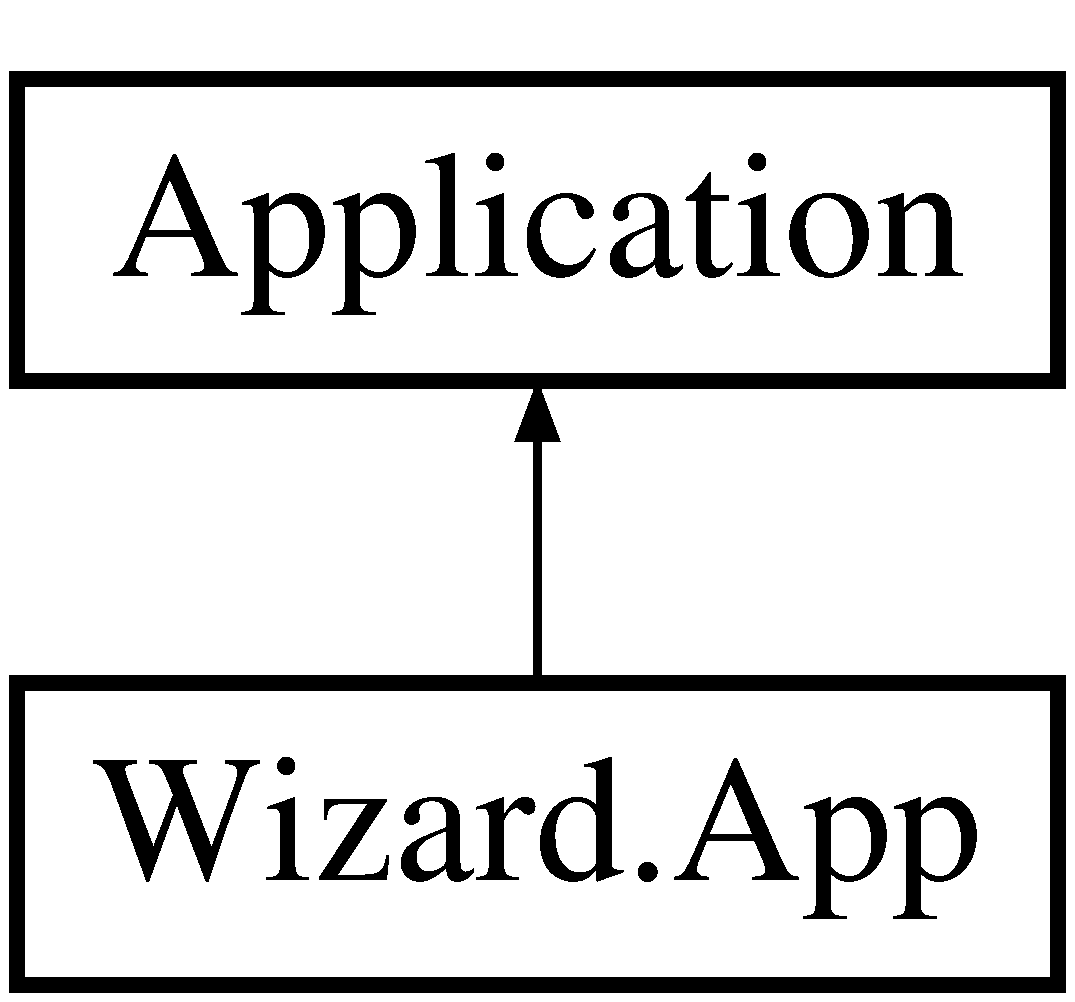
\includegraphics[height=2.000000cm]{class_wizard_1_1_app}
\end{center}
\end{figure}


\subsection{Detailed Description}
Interaction logic for App.\+xaml 



Definition at line 14 of file App.\+xaml.\+cs.



The documentation for this class was generated from the following file\+:\begin{DoxyCompactItemize}
\item 
C\+:/\+Users/\+Shehan Vanderputt/\+Downloads/\+Compressed/\+P\+E\+D\+Scanner-\/master/\+P\+E\+D\+Scanner-\/master/\+P\+E\+D\+Scanner\+G\+U\+I\+W\+P\+F/\+P\+E\+D\+Scanner/\+P\+E\+D\+Scanner/App.\+xaml.\+cs\end{DoxyCompactItemize}

\hypertarget{class_p_e_d_scanner_lib_1_1_objects_1_1_dependecies_object}{}\section{P\+E\+D\+Scanner\+Lib.\+Objects.\+Dependecies\+Object Class Reference}
\label{class_p_e_d_scanner_lib_1_1_objects_1_1_dependecies_object}\index{P\+E\+D\+Scanner\+Lib.\+Objects.\+Dependecies\+Object@{P\+E\+D\+Scanner\+Lib.\+Objects.\+Dependecies\+Object}}
\subsection*{Public Member Functions}
\begin{DoxyCompactItemize}
\item 
\mbox{\Hypertarget{class_p_e_d_scanner_lib_1_1_objects_1_1_dependecies_object_a10fa13dba74ca4133473412ef8cac23f}\label{class_p_e_d_scanner_lib_1_1_objects_1_1_dependecies_object_a10fa13dba74ca4133473412ef8cac23f}} 
{\bfseries Dependecies\+Object} (string dependency\+Name, bool is\+Loaded)
\end{DoxyCompactItemize}
\subsection*{Properties}
\begin{DoxyCompactItemize}
\item 
\mbox{\Hypertarget{class_p_e_d_scanner_lib_1_1_objects_1_1_dependecies_object_a95c794338f70edb119b3b6a61cad0ede}\label{class_p_e_d_scanner_lib_1_1_objects_1_1_dependecies_object_a95c794338f70edb119b3b6a61cad0ede}} 
string {\bfseries Dependency\+Name}\hspace{0.3cm}{\ttfamily  \mbox{[}get, set\mbox{]}}
\item 
\mbox{\Hypertarget{class_p_e_d_scanner_lib_1_1_objects_1_1_dependecies_object_a4a294f73c171a49a0b5dfd6a549f9ce0}\label{class_p_e_d_scanner_lib_1_1_objects_1_1_dependecies_object_a4a294f73c171a49a0b5dfd6a549f9ce0}} 
bool {\bfseries Is\+Loadable}\hspace{0.3cm}{\ttfamily  \mbox{[}get, set\mbox{]}}
\end{DoxyCompactItemize}


\subsection{Detailed Description}


Definition at line 49 of file P\+E\+Objects.\+cs.



The documentation for this class was generated from the following file\+:\begin{DoxyCompactItemize}
\item 
C\+:/\+Users/\+Shehan Vanderputt/\+Downloads/\+Compressed/\+P\+E\+D\+Scanner-\/master/\+P\+E\+D\+Scanner-\/master/\+P\+E\+D\+Scanner\+Lib/\+P\+E\+D\+Scanner\+Lib/P\+E\+Objects.\+cs\end{DoxyCompactItemize}

\hypertarget{class_p_e_d_scanner_lib_1_1_objects_1_1_directory_object}{}\section{P\+E\+D\+Scanner\+Lib.\+Objects.\+Directory\+Object Class Reference}
\label{class_p_e_d_scanner_lib_1_1_objects_1_1_directory_object}\index{P\+E\+D\+Scanner\+Lib.\+Objects.\+Directory\+Object@{P\+E\+D\+Scanner\+Lib.\+Objects.\+Directory\+Object}}
\subsection*{Public Member Functions}
\begin{DoxyCompactItemize}
\item 
\mbox{\Hypertarget{class_p_e_d_scanner_lib_1_1_objects_1_1_directory_object_a2e78a7cf87fd2cab2acb27a16f5671f8}\label{class_p_e_d_scanner_lib_1_1_objects_1_1_directory_object_a2e78a7cf87fd2cab2acb27a16f5671f8}} 
{\bfseries Directory\+Object} (string name, U\+Int32 R\+VA, U\+Int32 Size)
\end{DoxyCompactItemize}
\subsection*{Properties}
\begin{DoxyCompactItemize}
\item 
\mbox{\Hypertarget{class_p_e_d_scanner_lib_1_1_objects_1_1_directory_object_a2e270b3d714f66da57e23f32a975ef93}\label{class_p_e_d_scanner_lib_1_1_objects_1_1_directory_object_a2e270b3d714f66da57e23f32a975ef93}} 
string {\bfseries Name}\hspace{0.3cm}{\ttfamily  \mbox{[}get, set\mbox{]}}
\item 
\mbox{\Hypertarget{class_p_e_d_scanner_lib_1_1_objects_1_1_directory_object_ae7492459735714f502cc4efdf06eaac6}\label{class_p_e_d_scanner_lib_1_1_objects_1_1_directory_object_ae7492459735714f502cc4efdf06eaac6}} 
U\+Int32 {\bfseries R\+VA}\hspace{0.3cm}{\ttfamily  \mbox{[}get, set\mbox{]}}
\item 
\mbox{\Hypertarget{class_p_e_d_scanner_lib_1_1_objects_1_1_directory_object_aab914d383a39c0a577aed7723ae2c175}\label{class_p_e_d_scanner_lib_1_1_objects_1_1_directory_object_aab914d383a39c0a577aed7723ae2c175}} 
U\+Int32 {\bfseries Size}\hspace{0.3cm}{\ttfamily  \mbox{[}get, set\mbox{]}}
\end{DoxyCompactItemize}


\subsection{Detailed Description}


Definition at line 79 of file P\+E\+Objects.\+cs.



The documentation for this class was generated from the following file\+:\begin{DoxyCompactItemize}
\item 
C\+:/\+Users/\+Shehan Vanderputt/\+Downloads/\+Compressed/\+P\+E\+D\+Scanner-\/master/\+P\+E\+D\+Scanner-\/master/\+P\+E\+D\+Scanner\+Lib/\+P\+E\+D\+Scanner\+Lib/P\+E\+Objects.\+cs\end{DoxyCompactItemize}

\hypertarget{class_p_e_d_scanner_lib_1_1_objects_1_1_error_object}{}\section{P\+E\+D\+Scanner\+Lib.\+Objects.\+Error\+Object Class Reference}
\label{class_p_e_d_scanner_lib_1_1_objects_1_1_error_object}\index{P\+E\+D\+Scanner\+Lib.\+Objects.\+Error\+Object@{P\+E\+D\+Scanner\+Lib.\+Objects.\+Error\+Object}}
\subsection*{Public Member Functions}
\begin{DoxyCompactItemize}
\item 
\mbox{\Hypertarget{class_p_e_d_scanner_lib_1_1_objects_1_1_error_object_a0d16e01ee2b3700b16a171edb1d61ca7}\label{class_p_e_d_scanner_lib_1_1_objects_1_1_error_object_a0d16e01ee2b3700b16a171edb1d61ca7}} 
{\bfseries Error\+Object} (string dependency\+Name, string error)
\end{DoxyCompactItemize}
\subsection*{Properties}
\begin{DoxyCompactItemize}
\item 
\mbox{\Hypertarget{class_p_e_d_scanner_lib_1_1_objects_1_1_error_object_a394073acfe0088e73b71caf7646be09e}\label{class_p_e_d_scanner_lib_1_1_objects_1_1_error_object_a394073acfe0088e73b71caf7646be09e}} 
string {\bfseries Dependency\+Name}\hspace{0.3cm}{\ttfamily  \mbox{[}get, set\mbox{]}}
\item 
\mbox{\Hypertarget{class_p_e_d_scanner_lib_1_1_objects_1_1_error_object_ac58001f4e2bdef45cbda8c240297ddf0}\label{class_p_e_d_scanner_lib_1_1_objects_1_1_error_object_ac58001f4e2bdef45cbda8c240297ddf0}} 
string {\bfseries Error}\hspace{0.3cm}{\ttfamily  \mbox{[}get, set\mbox{]}}
\end{DoxyCompactItemize}


\subsection{Detailed Description}


Definition at line 16 of file P\+E\+Objects.\+cs.



The documentation for this class was generated from the following file\+:\begin{DoxyCompactItemize}
\item 
C\+:/\+Users/\+Shehan Vanderputt/\+Downloads/\+Compressed/\+P\+E\+D\+Scanner-\/master/\+P\+E\+D\+Scanner-\/master/\+P\+E\+D\+Scanner\+Lib/\+P\+E\+D\+Scanner\+Lib/P\+E\+Objects.\+cs\end{DoxyCompactItemize}

\hypertarget{class_objects_1_1_export_object}{}\section{Objects.\+Export\+Object Class Reference}
\label{class_objects_1_1_export_object}\index{Objects.\+Export\+Object@{Objects.\+Export\+Object}}
\subsection*{Public Member Functions}
\begin{DoxyCompactItemize}
\item 
\mbox{\Hypertarget{class_objects_1_1_export_object_a4eff4f8b60598d4b697d2d4c81f4472e}\label{class_objects_1_1_export_object_a4eff4f8b60598d4b697d2d4c81f4472e}} 
{\bfseries Export\+Object} (List$<$ \mbox{\hyperlink{class_objects_1_1_function_object}{Function\+Object}} $>$ list)
\item 
\mbox{\Hypertarget{class_objects_1_1_export_object_a4eff4f8b60598d4b697d2d4c81f4472e}\label{class_objects_1_1_export_object_a4eff4f8b60598d4b697d2d4c81f4472e}} 
{\bfseries Export\+Object} (List$<$ \mbox{\hyperlink{class_objects_1_1_function_object}{Function\+Object}} $>$ list)
\end{DoxyCompactItemize}
\subsection*{Properties}
\begin{DoxyCompactItemize}
\item 
\mbox{\Hypertarget{class_objects_1_1_export_object_a916515e6630ee9bfd58ce11ab6833991}\label{class_objects_1_1_export_object_a916515e6630ee9bfd58ce11ab6833991}} 
List$<$ \mbox{\hyperlink{class_objects_1_1_function_object}{Function\+Object}} $>$ {\bfseries Export\+Function\+Object\+List}\hspace{0.3cm}{\ttfamily  \mbox{[}get, set\mbox{]}}
\end{DoxyCompactItemize}


\subsection{Detailed Description}


Definition at line 49 of file I\+P\+C\+Client.\+cs.



The documentation for this class was generated from the following files\+:\begin{DoxyCompactItemize}
\item 
C\+:/\+Users/\+Shehan Vanderputt/\+Downloads/\+Compressed/\+P\+E\+D\+Scanner-\/master/\+P\+E\+D\+Scanner-\/master/\+P\+E\+D\+Scanner\+Lib/\+P\+E\+D\+Scanner\+Lib/I\+P\+C\+Client.\+cs\item 
C\+:/\+Users/\+Shehan Vanderputt/\+Downloads/\+Compressed/\+P\+E\+D\+Scanner-\/master/\+P\+E\+D\+Scanner-\/master/\+Server64\+Bit\+Library/\+Server64\+Bit\+Library/Class1.\+cs\end{DoxyCompactItemize}

\hypertarget{class_objects_1_1_function_object}{}\section{Objects.\+Function\+Object Class Reference}
\label{class_objects_1_1_function_object}\index{Objects.\+Function\+Object@{Objects.\+Function\+Object}}
Inheritance diagram for Objects.\+Function\+Object\+:\begin{figure}[H]
\begin{center}
\leavevmode
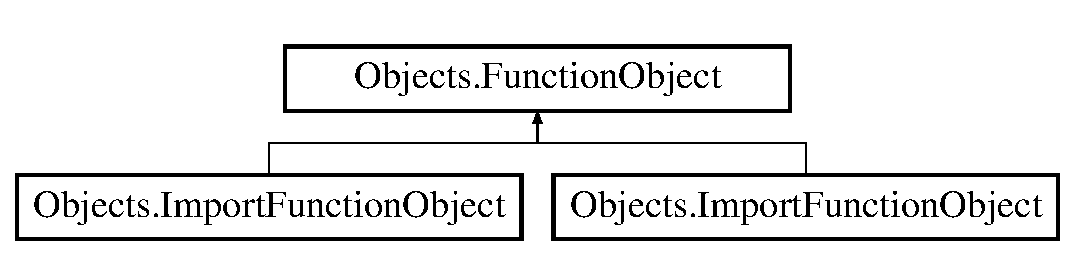
\includegraphics[height=2.000000cm]{class_objects_1_1_function_object}
\end{center}
\end{figure}
\subsection*{Public Member Functions}
\begin{DoxyCompactItemize}
\item 
\mbox{\Hypertarget{class_objects_1_1_function_object_a0e403a4988373d12b04c406e32537a37}\label{class_objects_1_1_function_object_a0e403a4988373d12b04c406e32537a37}} 
{\bfseries Function\+Object} (string function\+Name)
\item 
\mbox{\Hypertarget{class_objects_1_1_function_object_a0e403a4988373d12b04c406e32537a37}\label{class_objects_1_1_function_object_a0e403a4988373d12b04c406e32537a37}} 
{\bfseries Function\+Object} (string function\+Name)
\end{DoxyCompactItemize}
\subsection*{Properties}
\begin{DoxyCompactItemize}
\item 
\mbox{\Hypertarget{class_objects_1_1_function_object_a90ab3223aba8ad7b9c5fe920c35b5b08}\label{class_objects_1_1_function_object_a90ab3223aba8ad7b9c5fe920c35b5b08}} 
string {\bfseries Function}\hspace{0.3cm}{\ttfamily  \mbox{[}get, set\mbox{]}}
\item 
\mbox{\Hypertarget{class_objects_1_1_function_object_ad7a7be97d7003d8cd6e70c83d4b15178}\label{class_objects_1_1_function_object_ad7a7be97d7003d8cd6e70c83d4b15178}} 
List$<$ \mbox{\hyperlink{class_objects_1_1_function_object}{Function\+Object}} $>$ {\bfseries Function\+List}\hspace{0.3cm}{\ttfamily  \mbox{[}get, set\mbox{]}}
\end{DoxyCompactItemize}


\subsection{Detailed Description}


Definition at line 81 of file I\+P\+C\+Client.\+cs.



The documentation for this class was generated from the following files\+:\begin{DoxyCompactItemize}
\item 
C\+:/\+Users/\+Shehan Vanderputt/\+Downloads/\+Compressed/\+P\+E\+D\+Scanner-\/master/\+P\+E\+D\+Scanner-\/master/\+P\+E\+D\+Scanner\+Lib/\+P\+E\+D\+Scanner\+Lib/I\+P\+C\+Client.\+cs\item 
C\+:/\+Users/\+Shehan Vanderputt/\+Downloads/\+Compressed/\+P\+E\+D\+Scanner-\/master/\+P\+E\+D\+Scanner-\/master/\+Server64\+Bit\+Library/\+Server64\+Bit\+Library/Class1.\+cs\end{DoxyCompactItemize}

\hypertarget{class_p_e_d_scanner_lib_1_1_objects_1_1_header_object}{}\section{P\+E\+D\+Scanner\+Lib.\+Objects.\+Header\+Object Class Reference}
\label{class_p_e_d_scanner_lib_1_1_objects_1_1_header_object}\index{P\+E\+D\+Scanner\+Lib.\+Objects.\+Header\+Object@{P\+E\+D\+Scanner\+Lib.\+Objects.\+Header\+Object}}
\subsection*{Public Member Functions}
\begin{DoxyCompactItemize}
\item 
\mbox{\Hypertarget{class_p_e_d_scanner_lib_1_1_objects_1_1_header_object_ac42bc18545d3b2abbffa699480b0d015}\label{class_p_e_d_scanner_lib_1_1_objects_1_1_header_object_ac42bc18545d3b2abbffa699480b0d015}} 
{\bfseries Header\+Object} (string header\+Names, string value)
\end{DoxyCompactItemize}
\subsection*{Properties}
\begin{DoxyCompactItemize}
\item 
\mbox{\Hypertarget{class_p_e_d_scanner_lib_1_1_objects_1_1_header_object_aec97bbceceb864bdab14b4207146b82b}\label{class_p_e_d_scanner_lib_1_1_objects_1_1_header_object_aec97bbceceb864bdab14b4207146b82b}} 
string {\bfseries Name}\hspace{0.3cm}{\ttfamily  \mbox{[}get, set\mbox{]}}
\item 
\mbox{\Hypertarget{class_p_e_d_scanner_lib_1_1_objects_1_1_header_object_a729d5357389ac6defcc1f9add4aba35e}\label{class_p_e_d_scanner_lib_1_1_objects_1_1_header_object_a729d5357389ac6defcc1f9add4aba35e}} 
string {\bfseries Value}\hspace{0.3cm}{\ttfamily  \mbox{[}get, set\mbox{]}}
\end{DoxyCompactItemize}


\subsection{Detailed Description}


Definition at line 5 of file P\+E\+Objects.\+cs.



The documentation for this class was generated from the following file\+:\begin{DoxyCompactItemize}
\item 
C\+:/\+Users/\+Shehan Vanderputt/\+Downloads/\+Compressed/\+P\+E\+D\+Scanner-\/master/\+P\+E\+D\+Scanner-\/master/\+P\+E\+D\+Scanner\+Lib/\+P\+E\+D\+Scanner\+Lib/P\+E\+Objects.\+cs\end{DoxyCompactItemize}

\hypertarget{struct_class_library_server_1_1_struct_1_1_pe_header_reader_1_1_i_m_a_g_e___d_a_t_a___d_i_r_e_c_t_o_r_y}{}\section{Class\+Library\+Server.\+Struct.\+Pe\+Header\+Reader.\+I\+M\+A\+G\+E\+\_\+\+D\+A\+T\+A\+\_\+\+D\+I\+R\+E\+C\+T\+O\+RY Struct Reference}
\label{struct_class_library_server_1_1_struct_1_1_pe_header_reader_1_1_i_m_a_g_e___d_a_t_a___d_i_r_e_c_t_o_r_y}\index{Class\+Library\+Server.\+Struct.\+Pe\+Header\+Reader.\+I\+M\+A\+G\+E\+\_\+\+D\+A\+T\+A\+\_\+\+D\+I\+R\+E\+C\+T\+O\+RY@{Class\+Library\+Server.\+Struct.\+Pe\+Header\+Reader.\+I\+M\+A\+G\+E\+\_\+\+D\+A\+T\+A\+\_\+\+D\+I\+R\+E\+C\+T\+O\+RY}}
\subsection*{Public Attributes}
\begin{DoxyCompactItemize}
\item 
\mbox{\Hypertarget{struct_class_library_server_1_1_struct_1_1_pe_header_reader_1_1_i_m_a_g_e___d_a_t_a___d_i_r_e_c_t_o_r_y_a3d22c79dd96add2fc7cbd2ed91bb6dcb}\label{struct_class_library_server_1_1_struct_1_1_pe_header_reader_1_1_i_m_a_g_e___d_a_t_a___d_i_r_e_c_t_o_r_y_a3d22c79dd96add2fc7cbd2ed91bb6dcb}} 
U\+Int32 {\bfseries Virtual\+Address}
\item 
\mbox{\Hypertarget{struct_class_library_server_1_1_struct_1_1_pe_header_reader_1_1_i_m_a_g_e___d_a_t_a___d_i_r_e_c_t_o_r_y_aadbd7802559a9b572fc0c00e122a306d}\label{struct_class_library_server_1_1_struct_1_1_pe_header_reader_1_1_i_m_a_g_e___d_a_t_a___d_i_r_e_c_t_o_r_y_aadbd7802559a9b572fc0c00e122a306d}} 
U\+Int32 {\bfseries Size}
\end{DoxyCompactItemize}


\subsection{Detailed Description}


Definition at line 443 of file Native\+Dll\+Structure.\+cs.



The documentation for this struct was generated from the following file\+:\begin{DoxyCompactItemize}
\item 
C\+:/\+Users/\+Shehan Vanderputt/\+Downloads/\+Compressed/\+P\+E\+D\+Scanner-\/master/\+P\+E\+D\+Scanner-\/master/\+Server64\+Bit\+Library/\+Server64\+Bit\+Library/Native\+Dll\+Structure.\+cs\end{DoxyCompactItemize}

\hypertarget{struct_p_e_d_scanner_lib_1_1_struct_1_1_pe_header_reader_1_1_i_m_a_g_e___d_a_t_a___d_i_r_e_c_t_o_r_y}{}\section{P\+E\+D\+Scanner\+Lib.\+Struct.\+Pe\+Header\+Reader.\+I\+M\+A\+G\+E\+\_\+\+D\+A\+T\+A\+\_\+\+D\+I\+R\+E\+C\+T\+O\+RY Struct Reference}
\label{struct_p_e_d_scanner_lib_1_1_struct_1_1_pe_header_reader_1_1_i_m_a_g_e___d_a_t_a___d_i_r_e_c_t_o_r_y}\index{P\+E\+D\+Scanner\+Lib.\+Struct.\+Pe\+Header\+Reader.\+I\+M\+A\+G\+E\+\_\+\+D\+A\+T\+A\+\_\+\+D\+I\+R\+E\+C\+T\+O\+RY@{P\+E\+D\+Scanner\+Lib.\+Struct.\+Pe\+Header\+Reader.\+I\+M\+A\+G\+E\+\_\+\+D\+A\+T\+A\+\_\+\+D\+I\+R\+E\+C\+T\+O\+RY}}
\subsection*{Public Attributes}
\begin{DoxyCompactItemize}
\item 
\mbox{\Hypertarget{struct_p_e_d_scanner_lib_1_1_struct_1_1_pe_header_reader_1_1_i_m_a_g_e___d_a_t_a___d_i_r_e_c_t_o_r_y_af52e7d64352aa6ecf22232d3670fe089}\label{struct_p_e_d_scanner_lib_1_1_struct_1_1_pe_header_reader_1_1_i_m_a_g_e___d_a_t_a___d_i_r_e_c_t_o_r_y_af52e7d64352aa6ecf22232d3670fe089}} 
U\+Int32 {\bfseries Virtual\+Address}
\item 
\mbox{\Hypertarget{struct_p_e_d_scanner_lib_1_1_struct_1_1_pe_header_reader_1_1_i_m_a_g_e___d_a_t_a___d_i_r_e_c_t_o_r_y_a656b04455d4d9815865e58ae7a9bab0c}\label{struct_p_e_d_scanner_lib_1_1_struct_1_1_pe_header_reader_1_1_i_m_a_g_e___d_a_t_a___d_i_r_e_c_t_o_r_y_a656b04455d4d9815865e58ae7a9bab0c}} 
U\+Int32 {\bfseries Size}
\end{DoxyCompactItemize}


\subsection{Detailed Description}


Definition at line 395 of file Native\+Dll\+Structs.\+cs.



The documentation for this struct was generated from the following file\+:\begin{DoxyCompactItemize}
\item 
C\+:/\+Users/\+Shehan Vanderputt/\+Downloads/\+Compressed/\+P\+E\+D\+Scanner-\/master/\+P\+E\+D\+Scanner-\/master/\+P\+E\+D\+Scanner\+Lib/\+P\+E\+D\+Scanner\+Lib/Native\+Dll\+Structs.\+cs\end{DoxyCompactItemize}

\hypertarget{struct_p_e_d_scanner_lib_1_1_struct_1_1_pe_header_reader_1_1_i_m_a_g_e___d_o_s___h_e_a_d_e_r}{}\section{P\+E\+D\+Scanner\+Lib.\+Struct.\+Pe\+Header\+Reader.\+I\+M\+A\+G\+E\+\_\+\+D\+O\+S\+\_\+\+H\+E\+A\+D\+ER Struct Reference}
\label{struct_p_e_d_scanner_lib_1_1_struct_1_1_pe_header_reader_1_1_i_m_a_g_e___d_o_s___h_e_a_d_e_r}\index{P\+E\+D\+Scanner\+Lib.\+Struct.\+Pe\+Header\+Reader.\+I\+M\+A\+G\+E\+\_\+\+D\+O\+S\+\_\+\+H\+E\+A\+D\+ER@{P\+E\+D\+Scanner\+Lib.\+Struct.\+Pe\+Header\+Reader.\+I\+M\+A\+G\+E\+\_\+\+D\+O\+S\+\_\+\+H\+E\+A\+D\+ER}}
\subsection*{Public Attributes}
\begin{DoxyCompactItemize}
\item 
\mbox{\Hypertarget{struct_p_e_d_scanner_lib_1_1_struct_1_1_pe_header_reader_1_1_i_m_a_g_e___d_o_s___h_e_a_d_e_r_aa44c5b2208da46264ad9fe1de8bd14b0}\label{struct_p_e_d_scanner_lib_1_1_struct_1_1_pe_header_reader_1_1_i_m_a_g_e___d_o_s___h_e_a_d_e_r_aa44c5b2208da46264ad9fe1de8bd14b0}} 
U\+Int16 {\bfseries e\+\_\+magic}
\item 
\mbox{\Hypertarget{struct_p_e_d_scanner_lib_1_1_struct_1_1_pe_header_reader_1_1_i_m_a_g_e___d_o_s___h_e_a_d_e_r_a7822d0411e7b6c1e78e4dfa26045a91d}\label{struct_p_e_d_scanner_lib_1_1_struct_1_1_pe_header_reader_1_1_i_m_a_g_e___d_o_s___h_e_a_d_e_r_a7822d0411e7b6c1e78e4dfa26045a91d}} 
U\+Int16 {\bfseries e\+\_\+cblp}
\item 
\mbox{\Hypertarget{struct_p_e_d_scanner_lib_1_1_struct_1_1_pe_header_reader_1_1_i_m_a_g_e___d_o_s___h_e_a_d_e_r_ac2f807a1758ce8a0370b325831844e3f}\label{struct_p_e_d_scanner_lib_1_1_struct_1_1_pe_header_reader_1_1_i_m_a_g_e___d_o_s___h_e_a_d_e_r_ac2f807a1758ce8a0370b325831844e3f}} 
U\+Int16 {\bfseries e\+\_\+cp}
\item 
\mbox{\Hypertarget{struct_p_e_d_scanner_lib_1_1_struct_1_1_pe_header_reader_1_1_i_m_a_g_e___d_o_s___h_e_a_d_e_r_a33b7f4f8b1dea490eb415808dbd7bcc1}\label{struct_p_e_d_scanner_lib_1_1_struct_1_1_pe_header_reader_1_1_i_m_a_g_e___d_o_s___h_e_a_d_e_r_a33b7f4f8b1dea490eb415808dbd7bcc1}} 
U\+Int16 {\bfseries e\+\_\+crlc}
\item 
\mbox{\Hypertarget{struct_p_e_d_scanner_lib_1_1_struct_1_1_pe_header_reader_1_1_i_m_a_g_e___d_o_s___h_e_a_d_e_r_aa3a1c299ef8c785a710c077b3283c30f}\label{struct_p_e_d_scanner_lib_1_1_struct_1_1_pe_header_reader_1_1_i_m_a_g_e___d_o_s___h_e_a_d_e_r_aa3a1c299ef8c785a710c077b3283c30f}} 
U\+Int16 {\bfseries e\+\_\+cparhdr}
\item 
\mbox{\Hypertarget{struct_p_e_d_scanner_lib_1_1_struct_1_1_pe_header_reader_1_1_i_m_a_g_e___d_o_s___h_e_a_d_e_r_adf7c28fde90a2e904e753d1e3a245c4c}\label{struct_p_e_d_scanner_lib_1_1_struct_1_1_pe_header_reader_1_1_i_m_a_g_e___d_o_s___h_e_a_d_e_r_adf7c28fde90a2e904e753d1e3a245c4c}} 
U\+Int16 {\bfseries e\+\_\+minalloc}
\item 
\mbox{\Hypertarget{struct_p_e_d_scanner_lib_1_1_struct_1_1_pe_header_reader_1_1_i_m_a_g_e___d_o_s___h_e_a_d_e_r_afbf5d793e838f06d49324979b46d437e}\label{struct_p_e_d_scanner_lib_1_1_struct_1_1_pe_header_reader_1_1_i_m_a_g_e___d_o_s___h_e_a_d_e_r_afbf5d793e838f06d49324979b46d437e}} 
U\+Int16 {\bfseries e\+\_\+maxalloc}
\item 
\mbox{\Hypertarget{struct_p_e_d_scanner_lib_1_1_struct_1_1_pe_header_reader_1_1_i_m_a_g_e___d_o_s___h_e_a_d_e_r_a6603fcc25e8f4b532821fa3f05b7e6e0}\label{struct_p_e_d_scanner_lib_1_1_struct_1_1_pe_header_reader_1_1_i_m_a_g_e___d_o_s___h_e_a_d_e_r_a6603fcc25e8f4b532821fa3f05b7e6e0}} 
U\+Int16 {\bfseries e\+\_\+ss}
\item 
\mbox{\Hypertarget{struct_p_e_d_scanner_lib_1_1_struct_1_1_pe_header_reader_1_1_i_m_a_g_e___d_o_s___h_e_a_d_e_r_ac093317d9f7e3d2e44c559a08c194612}\label{struct_p_e_d_scanner_lib_1_1_struct_1_1_pe_header_reader_1_1_i_m_a_g_e___d_o_s___h_e_a_d_e_r_ac093317d9f7e3d2e44c559a08c194612}} 
U\+Int16 {\bfseries e\+\_\+sp}
\item 
\mbox{\Hypertarget{struct_p_e_d_scanner_lib_1_1_struct_1_1_pe_header_reader_1_1_i_m_a_g_e___d_o_s___h_e_a_d_e_r_a57d18b9af5c78a7230844bb7f7b23c59}\label{struct_p_e_d_scanner_lib_1_1_struct_1_1_pe_header_reader_1_1_i_m_a_g_e___d_o_s___h_e_a_d_e_r_a57d18b9af5c78a7230844bb7f7b23c59}} 
U\+Int16 {\bfseries e\+\_\+csum}
\item 
\mbox{\Hypertarget{struct_p_e_d_scanner_lib_1_1_struct_1_1_pe_header_reader_1_1_i_m_a_g_e___d_o_s___h_e_a_d_e_r_a6e9ea245389014522c28e823c723f052}\label{struct_p_e_d_scanner_lib_1_1_struct_1_1_pe_header_reader_1_1_i_m_a_g_e___d_o_s___h_e_a_d_e_r_a6e9ea245389014522c28e823c723f052}} 
U\+Int16 {\bfseries e\+\_\+ip}
\item 
\mbox{\Hypertarget{struct_p_e_d_scanner_lib_1_1_struct_1_1_pe_header_reader_1_1_i_m_a_g_e___d_o_s___h_e_a_d_e_r_a810a224b0e3c60bc2ce73633ef1a45a4}\label{struct_p_e_d_scanner_lib_1_1_struct_1_1_pe_header_reader_1_1_i_m_a_g_e___d_o_s___h_e_a_d_e_r_a810a224b0e3c60bc2ce73633ef1a45a4}} 
U\+Int16 {\bfseries e\+\_\+cs}
\item 
\mbox{\Hypertarget{struct_p_e_d_scanner_lib_1_1_struct_1_1_pe_header_reader_1_1_i_m_a_g_e___d_o_s___h_e_a_d_e_r_ac29c978d17122bbd2fef31800551beb4}\label{struct_p_e_d_scanner_lib_1_1_struct_1_1_pe_header_reader_1_1_i_m_a_g_e___d_o_s___h_e_a_d_e_r_ac29c978d17122bbd2fef31800551beb4}} 
U\+Int16 {\bfseries e\+\_\+lfarlc}
\item 
\mbox{\Hypertarget{struct_p_e_d_scanner_lib_1_1_struct_1_1_pe_header_reader_1_1_i_m_a_g_e___d_o_s___h_e_a_d_e_r_ada0d5f405c8b2a1d18c7c69ac4bb547e}\label{struct_p_e_d_scanner_lib_1_1_struct_1_1_pe_header_reader_1_1_i_m_a_g_e___d_o_s___h_e_a_d_e_r_ada0d5f405c8b2a1d18c7c69ac4bb547e}} 
U\+Int16 {\bfseries e\+\_\+ovno}
\item 
\mbox{\Hypertarget{struct_p_e_d_scanner_lib_1_1_struct_1_1_pe_header_reader_1_1_i_m_a_g_e___d_o_s___h_e_a_d_e_r_ae61ca0cc6621b5d3c605703b310803c8}\label{struct_p_e_d_scanner_lib_1_1_struct_1_1_pe_header_reader_1_1_i_m_a_g_e___d_o_s___h_e_a_d_e_r_ae61ca0cc6621b5d3c605703b310803c8}} 
U\+Int16 {\bfseries e\+\_\+res\+\_\+0}
\item 
\mbox{\Hypertarget{struct_p_e_d_scanner_lib_1_1_struct_1_1_pe_header_reader_1_1_i_m_a_g_e___d_o_s___h_e_a_d_e_r_a775baf15ed17fb7d7cc6d8dcd347a21e}\label{struct_p_e_d_scanner_lib_1_1_struct_1_1_pe_header_reader_1_1_i_m_a_g_e___d_o_s___h_e_a_d_e_r_a775baf15ed17fb7d7cc6d8dcd347a21e}} 
U\+Int16 {\bfseries e\+\_\+res\+\_\+1}
\item 
\mbox{\Hypertarget{struct_p_e_d_scanner_lib_1_1_struct_1_1_pe_header_reader_1_1_i_m_a_g_e___d_o_s___h_e_a_d_e_r_a23a03eeaddc9cc58653e4eee9b42bea2}\label{struct_p_e_d_scanner_lib_1_1_struct_1_1_pe_header_reader_1_1_i_m_a_g_e___d_o_s___h_e_a_d_e_r_a23a03eeaddc9cc58653e4eee9b42bea2}} 
U\+Int16 {\bfseries e\+\_\+res\+\_\+2}
\item 
\mbox{\Hypertarget{struct_p_e_d_scanner_lib_1_1_struct_1_1_pe_header_reader_1_1_i_m_a_g_e___d_o_s___h_e_a_d_e_r_a0911a560576444ef56d575ea4c50b69f}\label{struct_p_e_d_scanner_lib_1_1_struct_1_1_pe_header_reader_1_1_i_m_a_g_e___d_o_s___h_e_a_d_e_r_a0911a560576444ef56d575ea4c50b69f}} 
U\+Int16 {\bfseries e\+\_\+res\+\_\+3}
\item 
\mbox{\Hypertarget{struct_p_e_d_scanner_lib_1_1_struct_1_1_pe_header_reader_1_1_i_m_a_g_e___d_o_s___h_e_a_d_e_r_a53ce0f8b23fc880da3d9cbe79f2a4ce3}\label{struct_p_e_d_scanner_lib_1_1_struct_1_1_pe_header_reader_1_1_i_m_a_g_e___d_o_s___h_e_a_d_e_r_a53ce0f8b23fc880da3d9cbe79f2a4ce3}} 
U\+Int16 {\bfseries e\+\_\+oemid}
\item 
\mbox{\Hypertarget{struct_p_e_d_scanner_lib_1_1_struct_1_1_pe_header_reader_1_1_i_m_a_g_e___d_o_s___h_e_a_d_e_r_afe7b83f4d196c44a22dc95671a6f6f43}\label{struct_p_e_d_scanner_lib_1_1_struct_1_1_pe_header_reader_1_1_i_m_a_g_e___d_o_s___h_e_a_d_e_r_afe7b83f4d196c44a22dc95671a6f6f43}} 
U\+Int16 {\bfseries e\+\_\+oeminfo}
\item 
\mbox{\Hypertarget{struct_p_e_d_scanner_lib_1_1_struct_1_1_pe_header_reader_1_1_i_m_a_g_e___d_o_s___h_e_a_d_e_r_add2675a38a7293c0e9baeddedc93d696}\label{struct_p_e_d_scanner_lib_1_1_struct_1_1_pe_header_reader_1_1_i_m_a_g_e___d_o_s___h_e_a_d_e_r_add2675a38a7293c0e9baeddedc93d696}} 
U\+Int16 {\bfseries e\+\_\+res2\+\_\+0}
\item 
\mbox{\Hypertarget{struct_p_e_d_scanner_lib_1_1_struct_1_1_pe_header_reader_1_1_i_m_a_g_e___d_o_s___h_e_a_d_e_r_ae3472a691bf61168b626779e75947ead}\label{struct_p_e_d_scanner_lib_1_1_struct_1_1_pe_header_reader_1_1_i_m_a_g_e___d_o_s___h_e_a_d_e_r_ae3472a691bf61168b626779e75947ead}} 
U\+Int16 {\bfseries e\+\_\+res2\+\_\+1}
\item 
\mbox{\Hypertarget{struct_p_e_d_scanner_lib_1_1_struct_1_1_pe_header_reader_1_1_i_m_a_g_e___d_o_s___h_e_a_d_e_r_a78c9097c10d5929c4742b43512cb6772}\label{struct_p_e_d_scanner_lib_1_1_struct_1_1_pe_header_reader_1_1_i_m_a_g_e___d_o_s___h_e_a_d_e_r_a78c9097c10d5929c4742b43512cb6772}} 
U\+Int16 {\bfseries e\+\_\+res2\+\_\+2}
\item 
\mbox{\Hypertarget{struct_p_e_d_scanner_lib_1_1_struct_1_1_pe_header_reader_1_1_i_m_a_g_e___d_o_s___h_e_a_d_e_r_ac9dc4ee614688be21db1bffd8cc96d89}\label{struct_p_e_d_scanner_lib_1_1_struct_1_1_pe_header_reader_1_1_i_m_a_g_e___d_o_s___h_e_a_d_e_r_ac9dc4ee614688be21db1bffd8cc96d89}} 
U\+Int16 {\bfseries e\+\_\+res2\+\_\+3}
\item 
\mbox{\Hypertarget{struct_p_e_d_scanner_lib_1_1_struct_1_1_pe_header_reader_1_1_i_m_a_g_e___d_o_s___h_e_a_d_e_r_aff0a2571fde3be8cfe63c9986ec177f6}\label{struct_p_e_d_scanner_lib_1_1_struct_1_1_pe_header_reader_1_1_i_m_a_g_e___d_o_s___h_e_a_d_e_r_aff0a2571fde3be8cfe63c9986ec177f6}} 
U\+Int16 {\bfseries e\+\_\+res2\+\_\+4}
\item 
\mbox{\Hypertarget{struct_p_e_d_scanner_lib_1_1_struct_1_1_pe_header_reader_1_1_i_m_a_g_e___d_o_s___h_e_a_d_e_r_aa8d16acf20933c81cca1ec70161445e7}\label{struct_p_e_d_scanner_lib_1_1_struct_1_1_pe_header_reader_1_1_i_m_a_g_e___d_o_s___h_e_a_d_e_r_aa8d16acf20933c81cca1ec70161445e7}} 
U\+Int16 {\bfseries e\+\_\+res2\+\_\+5}
\item 
\mbox{\Hypertarget{struct_p_e_d_scanner_lib_1_1_struct_1_1_pe_header_reader_1_1_i_m_a_g_e___d_o_s___h_e_a_d_e_r_a00258e2693039d041132fcc980b034ce}\label{struct_p_e_d_scanner_lib_1_1_struct_1_1_pe_header_reader_1_1_i_m_a_g_e___d_o_s___h_e_a_d_e_r_a00258e2693039d041132fcc980b034ce}} 
U\+Int16 {\bfseries e\+\_\+res2\+\_\+6}
\item 
\mbox{\Hypertarget{struct_p_e_d_scanner_lib_1_1_struct_1_1_pe_header_reader_1_1_i_m_a_g_e___d_o_s___h_e_a_d_e_r_a5ea579905415b684355b8ad141482fad}\label{struct_p_e_d_scanner_lib_1_1_struct_1_1_pe_header_reader_1_1_i_m_a_g_e___d_o_s___h_e_a_d_e_r_a5ea579905415b684355b8ad141482fad}} 
U\+Int16 {\bfseries e\+\_\+res2\+\_\+7}
\item 
\mbox{\Hypertarget{struct_p_e_d_scanner_lib_1_1_struct_1_1_pe_header_reader_1_1_i_m_a_g_e___d_o_s___h_e_a_d_e_r_a5b59876ee5fea92c9f21149179522b89}\label{struct_p_e_d_scanner_lib_1_1_struct_1_1_pe_header_reader_1_1_i_m_a_g_e___d_o_s___h_e_a_d_e_r_a5b59876ee5fea92c9f21149179522b89}} 
U\+Int16 {\bfseries e\+\_\+res2\+\_\+8}
\item 
\mbox{\Hypertarget{struct_p_e_d_scanner_lib_1_1_struct_1_1_pe_header_reader_1_1_i_m_a_g_e___d_o_s___h_e_a_d_e_r_a6a812669202cfa3cfb3229fe8a13f1eb}\label{struct_p_e_d_scanner_lib_1_1_struct_1_1_pe_header_reader_1_1_i_m_a_g_e___d_o_s___h_e_a_d_e_r_a6a812669202cfa3cfb3229fe8a13f1eb}} 
U\+Int16 {\bfseries e\+\_\+res2\+\_\+9}
\item 
\mbox{\Hypertarget{struct_p_e_d_scanner_lib_1_1_struct_1_1_pe_header_reader_1_1_i_m_a_g_e___d_o_s___h_e_a_d_e_r_a5d2de752b108e5ca77ba4ee79ba7f5b5}\label{struct_p_e_d_scanner_lib_1_1_struct_1_1_pe_header_reader_1_1_i_m_a_g_e___d_o_s___h_e_a_d_e_r_a5d2de752b108e5ca77ba4ee79ba7f5b5}} 
U\+Int32 {\bfseries e\+\_\+lfanew}
\end{DoxyCompactItemize}


\subsection{Detailed Description}


Definition at line 359 of file Native\+Dll\+Structs.\+cs.



The documentation for this struct was generated from the following file\+:\begin{DoxyCompactItemize}
\item 
C\+:/\+Users/\+Shehan Vanderputt/\+Downloads/\+Compressed/\+P\+E\+D\+Scanner-\/master/\+P\+E\+D\+Scanner-\/master/\+P\+E\+D\+Scanner\+Lib/\+P\+E\+D\+Scanner\+Lib/Native\+Dll\+Structs.\+cs\end{DoxyCompactItemize}

\hypertarget{struct_class_library_server_1_1_struct_1_1_pe_header_reader_1_1_i_m_a_g_e___d_o_s___h_e_a_d_e_r}{}\section{Class\+Library\+Server.\+Struct.\+Pe\+Header\+Reader.\+I\+M\+A\+G\+E\+\_\+\+D\+O\+S\+\_\+\+H\+E\+A\+D\+ER Struct Reference}
\label{struct_class_library_server_1_1_struct_1_1_pe_header_reader_1_1_i_m_a_g_e___d_o_s___h_e_a_d_e_r}\index{Class\+Library\+Server.\+Struct.\+Pe\+Header\+Reader.\+I\+M\+A\+G\+E\+\_\+\+D\+O\+S\+\_\+\+H\+E\+A\+D\+ER@{Class\+Library\+Server.\+Struct.\+Pe\+Header\+Reader.\+I\+M\+A\+G\+E\+\_\+\+D\+O\+S\+\_\+\+H\+E\+A\+D\+ER}}
\subsection*{Public Attributes}
\begin{DoxyCompactItemize}
\item 
\mbox{\Hypertarget{struct_class_library_server_1_1_struct_1_1_pe_header_reader_1_1_i_m_a_g_e___d_o_s___h_e_a_d_e_r_a74e5692d7f3acaa42800784828bcb36f}\label{struct_class_library_server_1_1_struct_1_1_pe_header_reader_1_1_i_m_a_g_e___d_o_s___h_e_a_d_e_r_a74e5692d7f3acaa42800784828bcb36f}} 
U\+Int16 {\bfseries e\+\_\+magic}
\item 
\mbox{\Hypertarget{struct_class_library_server_1_1_struct_1_1_pe_header_reader_1_1_i_m_a_g_e___d_o_s___h_e_a_d_e_r_a9c90b111114b842fa7221b36e7a1ab85}\label{struct_class_library_server_1_1_struct_1_1_pe_header_reader_1_1_i_m_a_g_e___d_o_s___h_e_a_d_e_r_a9c90b111114b842fa7221b36e7a1ab85}} 
U\+Int16 {\bfseries e\+\_\+cblp}
\item 
\mbox{\Hypertarget{struct_class_library_server_1_1_struct_1_1_pe_header_reader_1_1_i_m_a_g_e___d_o_s___h_e_a_d_e_r_a1da1509195356b66e3811b0ffafe89ca}\label{struct_class_library_server_1_1_struct_1_1_pe_header_reader_1_1_i_m_a_g_e___d_o_s___h_e_a_d_e_r_a1da1509195356b66e3811b0ffafe89ca}} 
U\+Int16 {\bfseries e\+\_\+cp}
\item 
\mbox{\Hypertarget{struct_class_library_server_1_1_struct_1_1_pe_header_reader_1_1_i_m_a_g_e___d_o_s___h_e_a_d_e_r_a5c3208dd37eeb78cc291077f335c1803}\label{struct_class_library_server_1_1_struct_1_1_pe_header_reader_1_1_i_m_a_g_e___d_o_s___h_e_a_d_e_r_a5c3208dd37eeb78cc291077f335c1803}} 
U\+Int16 {\bfseries e\+\_\+crlc}
\item 
\mbox{\Hypertarget{struct_class_library_server_1_1_struct_1_1_pe_header_reader_1_1_i_m_a_g_e___d_o_s___h_e_a_d_e_r_a7375136cc5be5d95ad4612320711b931}\label{struct_class_library_server_1_1_struct_1_1_pe_header_reader_1_1_i_m_a_g_e___d_o_s___h_e_a_d_e_r_a7375136cc5be5d95ad4612320711b931}} 
U\+Int16 {\bfseries e\+\_\+cparhdr}
\item 
\mbox{\Hypertarget{struct_class_library_server_1_1_struct_1_1_pe_header_reader_1_1_i_m_a_g_e___d_o_s___h_e_a_d_e_r_a25b0c4f816bada3f564a75c09f6bf05b}\label{struct_class_library_server_1_1_struct_1_1_pe_header_reader_1_1_i_m_a_g_e___d_o_s___h_e_a_d_e_r_a25b0c4f816bada3f564a75c09f6bf05b}} 
U\+Int16 {\bfseries e\+\_\+minalloc}
\item 
\mbox{\Hypertarget{struct_class_library_server_1_1_struct_1_1_pe_header_reader_1_1_i_m_a_g_e___d_o_s___h_e_a_d_e_r_a4ae53b6c5f0fd9a0e841f9e2bb567a15}\label{struct_class_library_server_1_1_struct_1_1_pe_header_reader_1_1_i_m_a_g_e___d_o_s___h_e_a_d_e_r_a4ae53b6c5f0fd9a0e841f9e2bb567a15}} 
U\+Int16 {\bfseries e\+\_\+maxalloc}
\item 
\mbox{\Hypertarget{struct_class_library_server_1_1_struct_1_1_pe_header_reader_1_1_i_m_a_g_e___d_o_s___h_e_a_d_e_r_aa529b5bac909f761c7af2864d1fd3fdf}\label{struct_class_library_server_1_1_struct_1_1_pe_header_reader_1_1_i_m_a_g_e___d_o_s___h_e_a_d_e_r_aa529b5bac909f761c7af2864d1fd3fdf}} 
U\+Int16 {\bfseries e\+\_\+ss}
\item 
\mbox{\Hypertarget{struct_class_library_server_1_1_struct_1_1_pe_header_reader_1_1_i_m_a_g_e___d_o_s___h_e_a_d_e_r_ad4109d82c202e56dc37009772b4e9c60}\label{struct_class_library_server_1_1_struct_1_1_pe_header_reader_1_1_i_m_a_g_e___d_o_s___h_e_a_d_e_r_ad4109d82c202e56dc37009772b4e9c60}} 
U\+Int16 {\bfseries e\+\_\+sp}
\item 
\mbox{\Hypertarget{struct_class_library_server_1_1_struct_1_1_pe_header_reader_1_1_i_m_a_g_e___d_o_s___h_e_a_d_e_r_a3c6be57ef77ee52ad0350f5997499539}\label{struct_class_library_server_1_1_struct_1_1_pe_header_reader_1_1_i_m_a_g_e___d_o_s___h_e_a_d_e_r_a3c6be57ef77ee52ad0350f5997499539}} 
U\+Int16 {\bfseries e\+\_\+csum}
\item 
\mbox{\Hypertarget{struct_class_library_server_1_1_struct_1_1_pe_header_reader_1_1_i_m_a_g_e___d_o_s___h_e_a_d_e_r_acbbd97c774e2a4d5b00c9e29600a3aae}\label{struct_class_library_server_1_1_struct_1_1_pe_header_reader_1_1_i_m_a_g_e___d_o_s___h_e_a_d_e_r_acbbd97c774e2a4d5b00c9e29600a3aae}} 
U\+Int16 {\bfseries e\+\_\+ip}
\item 
\mbox{\Hypertarget{struct_class_library_server_1_1_struct_1_1_pe_header_reader_1_1_i_m_a_g_e___d_o_s___h_e_a_d_e_r_a412dd4885bfb5582f062943437189766}\label{struct_class_library_server_1_1_struct_1_1_pe_header_reader_1_1_i_m_a_g_e___d_o_s___h_e_a_d_e_r_a412dd4885bfb5582f062943437189766}} 
U\+Int16 {\bfseries e\+\_\+cs}
\item 
\mbox{\Hypertarget{struct_class_library_server_1_1_struct_1_1_pe_header_reader_1_1_i_m_a_g_e___d_o_s___h_e_a_d_e_r_adb543ddc6d6c1a91c97b082b3e9ee2ae}\label{struct_class_library_server_1_1_struct_1_1_pe_header_reader_1_1_i_m_a_g_e___d_o_s___h_e_a_d_e_r_adb543ddc6d6c1a91c97b082b3e9ee2ae}} 
U\+Int16 {\bfseries e\+\_\+lfarlc}
\item 
\mbox{\Hypertarget{struct_class_library_server_1_1_struct_1_1_pe_header_reader_1_1_i_m_a_g_e___d_o_s___h_e_a_d_e_r_ac8030abc9ef352302fd3a07278e017b8}\label{struct_class_library_server_1_1_struct_1_1_pe_header_reader_1_1_i_m_a_g_e___d_o_s___h_e_a_d_e_r_ac8030abc9ef352302fd3a07278e017b8}} 
U\+Int16 {\bfseries e\+\_\+ovno}
\item 
\mbox{\Hypertarget{struct_class_library_server_1_1_struct_1_1_pe_header_reader_1_1_i_m_a_g_e___d_o_s___h_e_a_d_e_r_afbad02b21d95e8f29407343d87f5bf1a}\label{struct_class_library_server_1_1_struct_1_1_pe_header_reader_1_1_i_m_a_g_e___d_o_s___h_e_a_d_e_r_afbad02b21d95e8f29407343d87f5bf1a}} 
U\+Int16 {\bfseries e\+\_\+res\+\_\+0}
\item 
\mbox{\Hypertarget{struct_class_library_server_1_1_struct_1_1_pe_header_reader_1_1_i_m_a_g_e___d_o_s___h_e_a_d_e_r_a78231b416446d1ffa122845178beaae8}\label{struct_class_library_server_1_1_struct_1_1_pe_header_reader_1_1_i_m_a_g_e___d_o_s___h_e_a_d_e_r_a78231b416446d1ffa122845178beaae8}} 
U\+Int16 {\bfseries e\+\_\+res\+\_\+1}
\item 
\mbox{\Hypertarget{struct_class_library_server_1_1_struct_1_1_pe_header_reader_1_1_i_m_a_g_e___d_o_s___h_e_a_d_e_r_a887c3fc427723e73d1fc60b3c3a85544}\label{struct_class_library_server_1_1_struct_1_1_pe_header_reader_1_1_i_m_a_g_e___d_o_s___h_e_a_d_e_r_a887c3fc427723e73d1fc60b3c3a85544}} 
U\+Int16 {\bfseries e\+\_\+res\+\_\+2}
\item 
\mbox{\Hypertarget{struct_class_library_server_1_1_struct_1_1_pe_header_reader_1_1_i_m_a_g_e___d_o_s___h_e_a_d_e_r_a505c8a98aa1c3acb3669755dcc06f7ab}\label{struct_class_library_server_1_1_struct_1_1_pe_header_reader_1_1_i_m_a_g_e___d_o_s___h_e_a_d_e_r_a505c8a98aa1c3acb3669755dcc06f7ab}} 
U\+Int16 {\bfseries e\+\_\+res\+\_\+3}
\item 
\mbox{\Hypertarget{struct_class_library_server_1_1_struct_1_1_pe_header_reader_1_1_i_m_a_g_e___d_o_s___h_e_a_d_e_r_a43ddab823a7cec7093cb9a5d3ac7c0b3}\label{struct_class_library_server_1_1_struct_1_1_pe_header_reader_1_1_i_m_a_g_e___d_o_s___h_e_a_d_e_r_a43ddab823a7cec7093cb9a5d3ac7c0b3}} 
U\+Int16 {\bfseries e\+\_\+oemid}
\item 
\mbox{\Hypertarget{struct_class_library_server_1_1_struct_1_1_pe_header_reader_1_1_i_m_a_g_e___d_o_s___h_e_a_d_e_r_a2e3bda3c3f0857e3725dd584ff343bcf}\label{struct_class_library_server_1_1_struct_1_1_pe_header_reader_1_1_i_m_a_g_e___d_o_s___h_e_a_d_e_r_a2e3bda3c3f0857e3725dd584ff343bcf}} 
U\+Int16 {\bfseries e\+\_\+oeminfo}
\item 
\mbox{\Hypertarget{struct_class_library_server_1_1_struct_1_1_pe_header_reader_1_1_i_m_a_g_e___d_o_s___h_e_a_d_e_r_a1fd011133cfa8c1345f4ebe35fb2025e}\label{struct_class_library_server_1_1_struct_1_1_pe_header_reader_1_1_i_m_a_g_e___d_o_s___h_e_a_d_e_r_a1fd011133cfa8c1345f4ebe35fb2025e}} 
U\+Int16 {\bfseries e\+\_\+res2\+\_\+0}
\item 
\mbox{\Hypertarget{struct_class_library_server_1_1_struct_1_1_pe_header_reader_1_1_i_m_a_g_e___d_o_s___h_e_a_d_e_r_acbca7380390608962ffc29f63abc9fca}\label{struct_class_library_server_1_1_struct_1_1_pe_header_reader_1_1_i_m_a_g_e___d_o_s___h_e_a_d_e_r_acbca7380390608962ffc29f63abc9fca}} 
U\+Int16 {\bfseries e\+\_\+res2\+\_\+1}
\item 
\mbox{\Hypertarget{struct_class_library_server_1_1_struct_1_1_pe_header_reader_1_1_i_m_a_g_e___d_o_s___h_e_a_d_e_r_acacbb30ff12d348054d9acfaae48ceda}\label{struct_class_library_server_1_1_struct_1_1_pe_header_reader_1_1_i_m_a_g_e___d_o_s___h_e_a_d_e_r_acacbb30ff12d348054d9acfaae48ceda}} 
U\+Int16 {\bfseries e\+\_\+res2\+\_\+2}
\item 
\mbox{\Hypertarget{struct_class_library_server_1_1_struct_1_1_pe_header_reader_1_1_i_m_a_g_e___d_o_s___h_e_a_d_e_r_aa4d6262f9d7a53fe0210ed139e6842a2}\label{struct_class_library_server_1_1_struct_1_1_pe_header_reader_1_1_i_m_a_g_e___d_o_s___h_e_a_d_e_r_aa4d6262f9d7a53fe0210ed139e6842a2}} 
U\+Int16 {\bfseries e\+\_\+res2\+\_\+3}
\item 
\mbox{\Hypertarget{struct_class_library_server_1_1_struct_1_1_pe_header_reader_1_1_i_m_a_g_e___d_o_s___h_e_a_d_e_r_a1f289b8ba96d09241c82fc878cb87b5e}\label{struct_class_library_server_1_1_struct_1_1_pe_header_reader_1_1_i_m_a_g_e___d_o_s___h_e_a_d_e_r_a1f289b8ba96d09241c82fc878cb87b5e}} 
U\+Int16 {\bfseries e\+\_\+res2\+\_\+4}
\item 
\mbox{\Hypertarget{struct_class_library_server_1_1_struct_1_1_pe_header_reader_1_1_i_m_a_g_e___d_o_s___h_e_a_d_e_r_a59a87e62edcc3d5549094837a669399c}\label{struct_class_library_server_1_1_struct_1_1_pe_header_reader_1_1_i_m_a_g_e___d_o_s___h_e_a_d_e_r_a59a87e62edcc3d5549094837a669399c}} 
U\+Int16 {\bfseries e\+\_\+res2\+\_\+5}
\item 
\mbox{\Hypertarget{struct_class_library_server_1_1_struct_1_1_pe_header_reader_1_1_i_m_a_g_e___d_o_s___h_e_a_d_e_r_a44571e6d1679458b7286533678c93567}\label{struct_class_library_server_1_1_struct_1_1_pe_header_reader_1_1_i_m_a_g_e___d_o_s___h_e_a_d_e_r_a44571e6d1679458b7286533678c93567}} 
U\+Int16 {\bfseries e\+\_\+res2\+\_\+6}
\item 
\mbox{\Hypertarget{struct_class_library_server_1_1_struct_1_1_pe_header_reader_1_1_i_m_a_g_e___d_o_s___h_e_a_d_e_r_a66ce40c47ccc8df825b35a3f96568759}\label{struct_class_library_server_1_1_struct_1_1_pe_header_reader_1_1_i_m_a_g_e___d_o_s___h_e_a_d_e_r_a66ce40c47ccc8df825b35a3f96568759}} 
U\+Int16 {\bfseries e\+\_\+res2\+\_\+7}
\item 
\mbox{\Hypertarget{struct_class_library_server_1_1_struct_1_1_pe_header_reader_1_1_i_m_a_g_e___d_o_s___h_e_a_d_e_r_a1b60a2587f5eec6575a6d30ccbaffd07}\label{struct_class_library_server_1_1_struct_1_1_pe_header_reader_1_1_i_m_a_g_e___d_o_s___h_e_a_d_e_r_a1b60a2587f5eec6575a6d30ccbaffd07}} 
U\+Int16 {\bfseries e\+\_\+res2\+\_\+8}
\item 
\mbox{\Hypertarget{struct_class_library_server_1_1_struct_1_1_pe_header_reader_1_1_i_m_a_g_e___d_o_s___h_e_a_d_e_r_aa47caa895825f176328a03446e9768cb}\label{struct_class_library_server_1_1_struct_1_1_pe_header_reader_1_1_i_m_a_g_e___d_o_s___h_e_a_d_e_r_aa47caa895825f176328a03446e9768cb}} 
U\+Int16 {\bfseries e\+\_\+res2\+\_\+9}
\item 
\mbox{\Hypertarget{struct_class_library_server_1_1_struct_1_1_pe_header_reader_1_1_i_m_a_g_e___d_o_s___h_e_a_d_e_r_a8ed4b3c04b3eed566e4a12003bff5882}\label{struct_class_library_server_1_1_struct_1_1_pe_header_reader_1_1_i_m_a_g_e___d_o_s___h_e_a_d_e_r_a8ed4b3c04b3eed566e4a12003bff5882}} 
U\+Int32 {\bfseries e\+\_\+lfanew}
\end{DoxyCompactItemize}


\subsection{Detailed Description}


Definition at line 407 of file Native\+Dll\+Structure.\+cs.



The documentation for this struct was generated from the following file\+:\begin{DoxyCompactItemize}
\item 
C\+:/\+Users/\+Shehan Vanderputt/\+Downloads/\+Compressed/\+P\+E\+D\+Scanner-\/master/\+P\+E\+D\+Scanner-\/master/\+Server64\+Bit\+Library/\+Server64\+Bit\+Library/Native\+Dll\+Structure.\+cs\end{DoxyCompactItemize}

\hypertarget{struct_p_e_d_scanner_lib_1_1_struct_1_1_i_m_a_g_e___e_x_p_o_r_t___d_i_r_e_c_t_o_r_y}{}\section{P\+E\+D\+Scanner\+Lib.\+Struct.\+I\+M\+A\+G\+E\+\_\+\+E\+X\+P\+O\+R\+T\+\_\+\+D\+I\+R\+E\+C\+T\+O\+RY Struct Reference}
\label{struct_p_e_d_scanner_lib_1_1_struct_1_1_i_m_a_g_e___e_x_p_o_r_t___d_i_r_e_c_t_o_r_y}\index{P\+E\+D\+Scanner\+Lib.\+Struct.\+I\+M\+A\+G\+E\+\_\+\+E\+X\+P\+O\+R\+T\+\_\+\+D\+I\+R\+E\+C\+T\+O\+RY@{P\+E\+D\+Scanner\+Lib.\+Struct.\+I\+M\+A\+G\+E\+\_\+\+E\+X\+P\+O\+R\+T\+\_\+\+D\+I\+R\+E\+C\+T\+O\+RY}}
\subsection*{Public Attributes}
\begin{DoxyCompactItemize}
\item 
\mbox{\Hypertarget{struct_p_e_d_scanner_lib_1_1_struct_1_1_i_m_a_g_e___e_x_p_o_r_t___d_i_r_e_c_t_o_r_y_ab29957807fee5e59499ecba7e8fc739f}\label{struct_p_e_d_scanner_lib_1_1_struct_1_1_i_m_a_g_e___e_x_p_o_r_t___d_i_r_e_c_t_o_r_y_ab29957807fee5e59499ecba7e8fc739f}} 
U\+Int32 {\bfseries Characteristics}
\item 
\mbox{\Hypertarget{struct_p_e_d_scanner_lib_1_1_struct_1_1_i_m_a_g_e___e_x_p_o_r_t___d_i_r_e_c_t_o_r_y_a522b3d8d8d4b0cdf746404c07b8d43b0}\label{struct_p_e_d_scanner_lib_1_1_struct_1_1_i_m_a_g_e___e_x_p_o_r_t___d_i_r_e_c_t_o_r_y_a522b3d8d8d4b0cdf746404c07b8d43b0}} 
U\+Int32 {\bfseries Time\+Date\+Stamp}
\item 
\mbox{\Hypertarget{struct_p_e_d_scanner_lib_1_1_struct_1_1_i_m_a_g_e___e_x_p_o_r_t___d_i_r_e_c_t_o_r_y_a352c5dd4b38218713848f362a70e846b}\label{struct_p_e_d_scanner_lib_1_1_struct_1_1_i_m_a_g_e___e_x_p_o_r_t___d_i_r_e_c_t_o_r_y_a352c5dd4b38218713848f362a70e846b}} 
U\+Int16 {\bfseries Major\+Version}
\item 
\mbox{\Hypertarget{struct_p_e_d_scanner_lib_1_1_struct_1_1_i_m_a_g_e___e_x_p_o_r_t___d_i_r_e_c_t_o_r_y_a5f91e2293951804c7c457ff882e7372a}\label{struct_p_e_d_scanner_lib_1_1_struct_1_1_i_m_a_g_e___e_x_p_o_r_t___d_i_r_e_c_t_o_r_y_a5f91e2293951804c7c457ff882e7372a}} 
U\+Int16 {\bfseries Minor\+Version}
\item 
\mbox{\Hypertarget{struct_p_e_d_scanner_lib_1_1_struct_1_1_i_m_a_g_e___e_x_p_o_r_t___d_i_r_e_c_t_o_r_y_ac01204bfb246e2c4aa3d2792d709c503}\label{struct_p_e_d_scanner_lib_1_1_struct_1_1_i_m_a_g_e___e_x_p_o_r_t___d_i_r_e_c_t_o_r_y_ac01204bfb246e2c4aa3d2792d709c503}} 
U\+Int32 {\bfseries Name}
\item 
\mbox{\Hypertarget{struct_p_e_d_scanner_lib_1_1_struct_1_1_i_m_a_g_e___e_x_p_o_r_t___d_i_r_e_c_t_o_r_y_a05a99ca6f000043b324616c88ed00895}\label{struct_p_e_d_scanner_lib_1_1_struct_1_1_i_m_a_g_e___e_x_p_o_r_t___d_i_r_e_c_t_o_r_y_a05a99ca6f000043b324616c88ed00895}} 
U\+Int32 {\bfseries Base}
\item 
\mbox{\Hypertarget{struct_p_e_d_scanner_lib_1_1_struct_1_1_i_m_a_g_e___e_x_p_o_r_t___d_i_r_e_c_t_o_r_y_afc364fa261a2873bb61ae841df851e0b}\label{struct_p_e_d_scanner_lib_1_1_struct_1_1_i_m_a_g_e___e_x_p_o_r_t___d_i_r_e_c_t_o_r_y_afc364fa261a2873bb61ae841df851e0b}} 
U\+Int32 {\bfseries Number\+Of\+Functions}
\item 
\mbox{\Hypertarget{struct_p_e_d_scanner_lib_1_1_struct_1_1_i_m_a_g_e___e_x_p_o_r_t___d_i_r_e_c_t_o_r_y_a1be960dec3ae268f47aac97c151045f1}\label{struct_p_e_d_scanner_lib_1_1_struct_1_1_i_m_a_g_e___e_x_p_o_r_t___d_i_r_e_c_t_o_r_y_a1be960dec3ae268f47aac97c151045f1}} 
U\+Int32 {\bfseries Number\+Of\+Names}
\item 
\mbox{\Hypertarget{struct_p_e_d_scanner_lib_1_1_struct_1_1_i_m_a_g_e___e_x_p_o_r_t___d_i_r_e_c_t_o_r_y_a9e250879f791f702988f8b338e236087}\label{struct_p_e_d_scanner_lib_1_1_struct_1_1_i_m_a_g_e___e_x_p_o_r_t___d_i_r_e_c_t_o_r_y_a9e250879f791f702988f8b338e236087}} 
U\+Int32 {\bfseries Address\+Of\+Functions}
\item 
\mbox{\Hypertarget{struct_p_e_d_scanner_lib_1_1_struct_1_1_i_m_a_g_e___e_x_p_o_r_t___d_i_r_e_c_t_o_r_y_a215647227cf196dee64347260e58e215}\label{struct_p_e_d_scanner_lib_1_1_struct_1_1_i_m_a_g_e___e_x_p_o_r_t___d_i_r_e_c_t_o_r_y_a215647227cf196dee64347260e58e215}} 
U\+Int32 {\bfseries Address\+Of\+Names}
\item 
\mbox{\Hypertarget{struct_p_e_d_scanner_lib_1_1_struct_1_1_i_m_a_g_e___e_x_p_o_r_t___d_i_r_e_c_t_o_r_y_a5cff9713e81a9ab662f9b2f262b9b4c3}\label{struct_p_e_d_scanner_lib_1_1_struct_1_1_i_m_a_g_e___e_x_p_o_r_t___d_i_r_e_c_t_o_r_y_a5cff9713e81a9ab662f9b2f262b9b4c3}} 
U\+Int32 {\bfseries Address\+Of\+Name\+Ordinals}
\end{DoxyCompactItemize}


\subsection{Detailed Description}


Definition at line 254 of file Native\+Dll\+Structs.\+cs.



The documentation for this struct was generated from the following file\+:\begin{DoxyCompactItemize}
\item 
C\+:/\+Users/\+Shehan Vanderputt/\+Downloads/\+Compressed/\+P\+E\+D\+Scanner-\/master/\+P\+E\+D\+Scanner-\/master/\+P\+E\+D\+Scanner\+Lib/\+P\+E\+D\+Scanner\+Lib/Native\+Dll\+Structs.\+cs\end{DoxyCompactItemize}

\hypertarget{struct_class_library_server_1_1_struct_1_1_i_m_a_g_e___e_x_p_o_r_t___d_i_r_e_c_t_o_r_y}{}\section{Class\+Library\+Server.\+Struct.\+I\+M\+A\+G\+E\+\_\+\+E\+X\+P\+O\+R\+T\+\_\+\+D\+I\+R\+E\+C\+T\+O\+RY Struct Reference}
\label{struct_class_library_server_1_1_struct_1_1_i_m_a_g_e___e_x_p_o_r_t___d_i_r_e_c_t_o_r_y}\index{Class\+Library\+Server.\+Struct.\+I\+M\+A\+G\+E\+\_\+\+E\+X\+P\+O\+R\+T\+\_\+\+D\+I\+R\+E\+C\+T\+O\+RY@{Class\+Library\+Server.\+Struct.\+I\+M\+A\+G\+E\+\_\+\+E\+X\+P\+O\+R\+T\+\_\+\+D\+I\+R\+E\+C\+T\+O\+RY}}
\subsection*{Public Attributes}
\begin{DoxyCompactItemize}
\item 
\mbox{\Hypertarget{struct_class_library_server_1_1_struct_1_1_i_m_a_g_e___e_x_p_o_r_t___d_i_r_e_c_t_o_r_y_a2c91066bb399be2cb65ab797b9cf2b42}\label{struct_class_library_server_1_1_struct_1_1_i_m_a_g_e___e_x_p_o_r_t___d_i_r_e_c_t_o_r_y_a2c91066bb399be2cb65ab797b9cf2b42}} 
U\+Int32 {\bfseries Characteristics}
\item 
\mbox{\Hypertarget{struct_class_library_server_1_1_struct_1_1_i_m_a_g_e___e_x_p_o_r_t___d_i_r_e_c_t_o_r_y_a5601f3475b74a38c7e759f76b18ca7e4}\label{struct_class_library_server_1_1_struct_1_1_i_m_a_g_e___e_x_p_o_r_t___d_i_r_e_c_t_o_r_y_a5601f3475b74a38c7e759f76b18ca7e4}} 
U\+Int32 {\bfseries Time\+Date\+Stamp}
\item 
\mbox{\Hypertarget{struct_class_library_server_1_1_struct_1_1_i_m_a_g_e___e_x_p_o_r_t___d_i_r_e_c_t_o_r_y_ad0bc442da82342372e5dd735776310f1}\label{struct_class_library_server_1_1_struct_1_1_i_m_a_g_e___e_x_p_o_r_t___d_i_r_e_c_t_o_r_y_ad0bc442da82342372e5dd735776310f1}} 
U\+Int16 {\bfseries Major\+Version}
\item 
\mbox{\Hypertarget{struct_class_library_server_1_1_struct_1_1_i_m_a_g_e___e_x_p_o_r_t___d_i_r_e_c_t_o_r_y_adc7219756dd73bb38636f49bc70a4a00}\label{struct_class_library_server_1_1_struct_1_1_i_m_a_g_e___e_x_p_o_r_t___d_i_r_e_c_t_o_r_y_adc7219756dd73bb38636f49bc70a4a00}} 
U\+Int16 {\bfseries Minor\+Version}
\item 
\mbox{\Hypertarget{struct_class_library_server_1_1_struct_1_1_i_m_a_g_e___e_x_p_o_r_t___d_i_r_e_c_t_o_r_y_ab78be00f226f6afe7074249fff29c13d}\label{struct_class_library_server_1_1_struct_1_1_i_m_a_g_e___e_x_p_o_r_t___d_i_r_e_c_t_o_r_y_ab78be00f226f6afe7074249fff29c13d}} 
U\+Int32 {\bfseries Name}
\item 
\mbox{\Hypertarget{struct_class_library_server_1_1_struct_1_1_i_m_a_g_e___e_x_p_o_r_t___d_i_r_e_c_t_o_r_y_af3ac56929590c73c7959bae604d77ae5}\label{struct_class_library_server_1_1_struct_1_1_i_m_a_g_e___e_x_p_o_r_t___d_i_r_e_c_t_o_r_y_af3ac56929590c73c7959bae604d77ae5}} 
U\+Int32 {\bfseries Base}
\item 
\mbox{\Hypertarget{struct_class_library_server_1_1_struct_1_1_i_m_a_g_e___e_x_p_o_r_t___d_i_r_e_c_t_o_r_y_a0e6a39dff02e298572ee4074917690b9}\label{struct_class_library_server_1_1_struct_1_1_i_m_a_g_e___e_x_p_o_r_t___d_i_r_e_c_t_o_r_y_a0e6a39dff02e298572ee4074917690b9}} 
U\+Int32 {\bfseries Number\+Of\+Functions}
\item 
\mbox{\Hypertarget{struct_class_library_server_1_1_struct_1_1_i_m_a_g_e___e_x_p_o_r_t___d_i_r_e_c_t_o_r_y_a1a1d259075793e3cc518be909b3d1e4b}\label{struct_class_library_server_1_1_struct_1_1_i_m_a_g_e___e_x_p_o_r_t___d_i_r_e_c_t_o_r_y_a1a1d259075793e3cc518be909b3d1e4b}} 
U\+Int32 {\bfseries Number\+Of\+Names}
\item 
\mbox{\Hypertarget{struct_class_library_server_1_1_struct_1_1_i_m_a_g_e___e_x_p_o_r_t___d_i_r_e_c_t_o_r_y_ae90f160fd1dcff7671427c2277f2a29d}\label{struct_class_library_server_1_1_struct_1_1_i_m_a_g_e___e_x_p_o_r_t___d_i_r_e_c_t_o_r_y_ae90f160fd1dcff7671427c2277f2a29d}} 
U\+Int32 {\bfseries Address\+Of\+Functions}
\item 
\mbox{\Hypertarget{struct_class_library_server_1_1_struct_1_1_i_m_a_g_e___e_x_p_o_r_t___d_i_r_e_c_t_o_r_y_adf8c46c4d841d9f381bcb6ee52d2e7e9}\label{struct_class_library_server_1_1_struct_1_1_i_m_a_g_e___e_x_p_o_r_t___d_i_r_e_c_t_o_r_y_adf8c46c4d841d9f381bcb6ee52d2e7e9}} 
U\+Int32 {\bfseries Address\+Of\+Names}
\item 
\mbox{\Hypertarget{struct_class_library_server_1_1_struct_1_1_i_m_a_g_e___e_x_p_o_r_t___d_i_r_e_c_t_o_r_y_ae1ef775787cf8ac4e2b8d0338b7fea70}\label{struct_class_library_server_1_1_struct_1_1_i_m_a_g_e___e_x_p_o_r_t___d_i_r_e_c_t_o_r_y_ae1ef775787cf8ac4e2b8d0338b7fea70}} 
U\+Int32 {\bfseries Address\+Of\+Name\+Ordinals}
\end{DoxyCompactItemize}


\subsection{Detailed Description}


Definition at line 295 of file Native\+Dll\+Structure.\+cs.



The documentation for this struct was generated from the following file\+:\begin{DoxyCompactItemize}
\item 
C\+:/\+Users/\+Shehan Vanderputt/\+Downloads/\+Compressed/\+P\+E\+D\+Scanner-\/master/\+P\+E\+D\+Scanner-\/master/\+Server64\+Bit\+Library/\+Server64\+Bit\+Library/Native\+Dll\+Structure.\+cs\end{DoxyCompactItemize}

\hypertarget{struct_p_e_d_scanner_lib_1_1_struct_1_1_i_m_a_g_e___f_i_l_e___h_e_a_d_e_r}{}\section{P\+E\+D\+Scanner\+Lib.\+Struct.\+I\+M\+A\+G\+E\+\_\+\+F\+I\+L\+E\+\_\+\+H\+E\+A\+D\+ER Struct Reference}
\label{struct_p_e_d_scanner_lib_1_1_struct_1_1_i_m_a_g_e___f_i_l_e___h_e_a_d_e_r}\index{P\+E\+D\+Scanner\+Lib.\+Struct.\+I\+M\+A\+G\+E\+\_\+\+F\+I\+L\+E\+\_\+\+H\+E\+A\+D\+ER@{P\+E\+D\+Scanner\+Lib.\+Struct.\+I\+M\+A\+G\+E\+\_\+\+F\+I\+L\+E\+\_\+\+H\+E\+A\+D\+ER}}
\subsection*{Public Attributes}
\begin{DoxyCompactItemize}
\item 
\mbox{\Hypertarget{struct_p_e_d_scanner_lib_1_1_struct_1_1_i_m_a_g_e___f_i_l_e___h_e_a_d_e_r_a1da52d9b7f2cc3ab26aec5ba95d47e56}\label{struct_p_e_d_scanner_lib_1_1_struct_1_1_i_m_a_g_e___f_i_l_e___h_e_a_d_e_r_a1da52d9b7f2cc3ab26aec5ba95d47e56}} 
U\+Int16 {\bfseries Machine}
\item 
\mbox{\Hypertarget{struct_p_e_d_scanner_lib_1_1_struct_1_1_i_m_a_g_e___f_i_l_e___h_e_a_d_e_r_afb170aad2439c4648e95d959a3cda816}\label{struct_p_e_d_scanner_lib_1_1_struct_1_1_i_m_a_g_e___f_i_l_e___h_e_a_d_e_r_afb170aad2439c4648e95d959a3cda816}} 
U\+Int16 {\bfseries Number\+Of\+Sections}
\item 
\mbox{\Hypertarget{struct_p_e_d_scanner_lib_1_1_struct_1_1_i_m_a_g_e___f_i_l_e___h_e_a_d_e_r_a635595bc92db9ca9b7f3bd0904b434cd}\label{struct_p_e_d_scanner_lib_1_1_struct_1_1_i_m_a_g_e___f_i_l_e___h_e_a_d_e_r_a635595bc92db9ca9b7f3bd0904b434cd}} 
U\+Int32 {\bfseries Time\+Date\+Stamp}
\item 
\mbox{\Hypertarget{struct_p_e_d_scanner_lib_1_1_struct_1_1_i_m_a_g_e___f_i_l_e___h_e_a_d_e_r_a3575de2b61fc6ff18e5559d667246cb2}\label{struct_p_e_d_scanner_lib_1_1_struct_1_1_i_m_a_g_e___f_i_l_e___h_e_a_d_e_r_a3575de2b61fc6ff18e5559d667246cb2}} 
U\+Int32 {\bfseries Pointer\+To\+Symbol\+Table}
\item 
\mbox{\Hypertarget{struct_p_e_d_scanner_lib_1_1_struct_1_1_i_m_a_g_e___f_i_l_e___h_e_a_d_e_r_a4d3554265f629d209e383e4295634bb9}\label{struct_p_e_d_scanner_lib_1_1_struct_1_1_i_m_a_g_e___f_i_l_e___h_e_a_d_e_r_a4d3554265f629d209e383e4295634bb9}} 
U\+Int32 {\bfseries Number\+Of\+Symbols}
\item 
\mbox{\Hypertarget{struct_p_e_d_scanner_lib_1_1_struct_1_1_i_m_a_g_e___f_i_l_e___h_e_a_d_e_r_a09da0aaa9db95fb2b995954d95472e1c}\label{struct_p_e_d_scanner_lib_1_1_struct_1_1_i_m_a_g_e___f_i_l_e___h_e_a_d_e_r_a09da0aaa9db95fb2b995954d95472e1c}} 
U\+Int16 {\bfseries Size\+Of\+Optional\+Header}
\item 
\mbox{\Hypertarget{struct_p_e_d_scanner_lib_1_1_struct_1_1_i_m_a_g_e___f_i_l_e___h_e_a_d_e_r_acbcad9556719d5c29878619e3c89ecc7}\label{struct_p_e_d_scanner_lib_1_1_struct_1_1_i_m_a_g_e___f_i_l_e___h_e_a_d_e_r_acbcad9556719d5c29878619e3c89ecc7}} 
U\+Int16 {\bfseries Characteristics}
\end{DoxyCompactItemize}


\subsection{Detailed Description}


Definition at line 288 of file Native\+Dll\+Structs.\+cs.



The documentation for this struct was generated from the following file\+:\begin{DoxyCompactItemize}
\item 
C\+:/\+Users/\+Shehan Vanderputt/\+Downloads/\+Compressed/\+P\+E\+D\+Scanner-\/master/\+P\+E\+D\+Scanner-\/master/\+P\+E\+D\+Scanner\+Lib/\+P\+E\+D\+Scanner\+Lib/Native\+Dll\+Structs.\+cs\end{DoxyCompactItemize}

\hypertarget{struct_class_library_server_1_1_struct_1_1_i_m_a_g_e___f_i_l_e___h_e_a_d_e_r}{}\section{Class\+Library\+Server.\+Struct.\+I\+M\+A\+G\+E\+\_\+\+F\+I\+L\+E\+\_\+\+H\+E\+A\+D\+ER Struct Reference}
\label{struct_class_library_server_1_1_struct_1_1_i_m_a_g_e___f_i_l_e___h_e_a_d_e_r}\index{Class\+Library\+Server.\+Struct.\+I\+M\+A\+G\+E\+\_\+\+F\+I\+L\+E\+\_\+\+H\+E\+A\+D\+ER@{Class\+Library\+Server.\+Struct.\+I\+M\+A\+G\+E\+\_\+\+F\+I\+L\+E\+\_\+\+H\+E\+A\+D\+ER}}
\subsection*{Public Attributes}
\begin{DoxyCompactItemize}
\item 
\mbox{\Hypertarget{struct_class_library_server_1_1_struct_1_1_i_m_a_g_e___f_i_l_e___h_e_a_d_e_r_aa5f813a18adfe7fb20fc92f09bfcb8d6}\label{struct_class_library_server_1_1_struct_1_1_i_m_a_g_e___f_i_l_e___h_e_a_d_e_r_aa5f813a18adfe7fb20fc92f09bfcb8d6}} 
U\+Int16 {\bfseries Machine}
\item 
\mbox{\Hypertarget{struct_class_library_server_1_1_struct_1_1_i_m_a_g_e___f_i_l_e___h_e_a_d_e_r_a619506e50151a69605107aee78c03409}\label{struct_class_library_server_1_1_struct_1_1_i_m_a_g_e___f_i_l_e___h_e_a_d_e_r_a619506e50151a69605107aee78c03409}} 
U\+Int16 {\bfseries Number\+Of\+Sections}
\item 
\mbox{\Hypertarget{struct_class_library_server_1_1_struct_1_1_i_m_a_g_e___f_i_l_e___h_e_a_d_e_r_a21b50d5e22e53caad31c36cda7a3a41d}\label{struct_class_library_server_1_1_struct_1_1_i_m_a_g_e___f_i_l_e___h_e_a_d_e_r_a21b50d5e22e53caad31c36cda7a3a41d}} 
U\+Int32 {\bfseries Time\+Date\+Stamp}
\item 
\mbox{\Hypertarget{struct_class_library_server_1_1_struct_1_1_i_m_a_g_e___f_i_l_e___h_e_a_d_e_r_a6cf208ef19fce49736eb6c6dc1f53fb9}\label{struct_class_library_server_1_1_struct_1_1_i_m_a_g_e___f_i_l_e___h_e_a_d_e_r_a6cf208ef19fce49736eb6c6dc1f53fb9}} 
U\+Int32 {\bfseries Pointer\+To\+Symbol\+Table}
\item 
\mbox{\Hypertarget{struct_class_library_server_1_1_struct_1_1_i_m_a_g_e___f_i_l_e___h_e_a_d_e_r_a15da069dbf8017b956bf0eec3f9b7b49}\label{struct_class_library_server_1_1_struct_1_1_i_m_a_g_e___f_i_l_e___h_e_a_d_e_r_a15da069dbf8017b956bf0eec3f9b7b49}} 
U\+Int32 {\bfseries Number\+Of\+Symbols}
\item 
\mbox{\Hypertarget{struct_class_library_server_1_1_struct_1_1_i_m_a_g_e___f_i_l_e___h_e_a_d_e_r_ac98815671d0d1e7369a7e0343dc66b10}\label{struct_class_library_server_1_1_struct_1_1_i_m_a_g_e___f_i_l_e___h_e_a_d_e_r_ac98815671d0d1e7369a7e0343dc66b10}} 
U\+Int16 {\bfseries Size\+Of\+Optional\+Header}
\item 
\mbox{\Hypertarget{struct_class_library_server_1_1_struct_1_1_i_m_a_g_e___f_i_l_e___h_e_a_d_e_r_ae731f184ccb479e4ec772ae62e281cdb}\label{struct_class_library_server_1_1_struct_1_1_i_m_a_g_e___f_i_l_e___h_e_a_d_e_r_ae731f184ccb479e4ec772ae62e281cdb}} 
U\+Int16 {\bfseries Characteristics}
\end{DoxyCompactItemize}


\subsection{Detailed Description}


Definition at line 329 of file Native\+Dll\+Structure.\+cs.



The documentation for this struct was generated from the following file\+:\begin{DoxyCompactItemize}
\item 
C\+:/\+Users/\+Shehan Vanderputt/\+Downloads/\+Compressed/\+P\+E\+D\+Scanner-\/master/\+P\+E\+D\+Scanner-\/master/\+Server64\+Bit\+Library/\+Server64\+Bit\+Library/Native\+Dll\+Structure.\+cs\end{DoxyCompactItemize}

\hypertarget{struct_p_e_d_scanner_lib_1_1_struct_1_1_pe_header_reader_1_1_i_m_a_g_e___i_m_p_o_r_t___b_y___n_a_m_e}{}\section{P\+E\+D\+Scanner\+Lib.\+Struct.\+Pe\+Header\+Reader.\+I\+M\+A\+G\+E\+\_\+\+I\+M\+P\+O\+R\+T\+\_\+\+B\+Y\+\_\+\+N\+A\+ME Struct Reference}
\label{struct_p_e_d_scanner_lib_1_1_struct_1_1_pe_header_reader_1_1_i_m_a_g_e___i_m_p_o_r_t___b_y___n_a_m_e}\index{P\+E\+D\+Scanner\+Lib.\+Struct.\+Pe\+Header\+Reader.\+I\+M\+A\+G\+E\+\_\+\+I\+M\+P\+O\+R\+T\+\_\+\+B\+Y\+\_\+\+N\+A\+ME@{P\+E\+D\+Scanner\+Lib.\+Struct.\+Pe\+Header\+Reader.\+I\+M\+A\+G\+E\+\_\+\+I\+M\+P\+O\+R\+T\+\_\+\+B\+Y\+\_\+\+N\+A\+ME}}
\subsection*{Public Attributes}
\begin{DoxyCompactItemize}
\item 
\mbox{\Hypertarget{struct_p_e_d_scanner_lib_1_1_struct_1_1_pe_header_reader_1_1_i_m_a_g_e___i_m_p_o_r_t___b_y___n_a_m_e_acec711cf65cfc2049990cf88010ef290}\label{struct_p_e_d_scanner_lib_1_1_struct_1_1_pe_header_reader_1_1_i_m_a_g_e___i_m_p_o_r_t___b_y___n_a_m_e_acec711cf65cfc2049990cf88010ef290}} 
ushort {\bfseries Hint}
\item 
\mbox{\Hypertarget{struct_p_e_d_scanner_lib_1_1_struct_1_1_pe_header_reader_1_1_i_m_a_g_e___i_m_p_o_r_t___b_y___n_a_m_e_a023c321cbfd2ce6e35595b370ddebd2c}\label{struct_p_e_d_scanner_lib_1_1_struct_1_1_pe_header_reader_1_1_i_m_a_g_e___i_m_p_o_r_t___b_y___n_a_m_e_a023c321cbfd2ce6e35595b370ddebd2c}} 
fixed char {\bfseries Name} \mbox{[}1\mbox{]}
\end{DoxyCompactItemize}


\subsection{Detailed Description}


Definition at line 441 of file Native\+Dll\+Structs.\+cs.



The documentation for this struct was generated from the following file\+:\begin{DoxyCompactItemize}
\item 
C\+:/\+Users/\+Shehan Vanderputt/\+Downloads/\+Compressed/\+P\+E\+D\+Scanner-\/master/\+P\+E\+D\+Scanner-\/master/\+P\+E\+D\+Scanner\+Lib/\+P\+E\+D\+Scanner\+Lib/Native\+Dll\+Structs.\+cs\end{DoxyCompactItemize}

\hypertarget{struct_class_library_server_1_1_struct_1_1_pe_header_reader_1_1_i_m_a_g_e___i_m_p_o_r_t___b_y___n_a_m_e}{}\section{Class\+Library\+Server.\+Struct.\+Pe\+Header\+Reader.\+I\+M\+A\+G\+E\+\_\+\+I\+M\+P\+O\+R\+T\+\_\+\+B\+Y\+\_\+\+N\+A\+ME Struct Reference}
\label{struct_class_library_server_1_1_struct_1_1_pe_header_reader_1_1_i_m_a_g_e___i_m_p_o_r_t___b_y___n_a_m_e}\index{Class\+Library\+Server.\+Struct.\+Pe\+Header\+Reader.\+I\+M\+A\+G\+E\+\_\+\+I\+M\+P\+O\+R\+T\+\_\+\+B\+Y\+\_\+\+N\+A\+ME@{Class\+Library\+Server.\+Struct.\+Pe\+Header\+Reader.\+I\+M\+A\+G\+E\+\_\+\+I\+M\+P\+O\+R\+T\+\_\+\+B\+Y\+\_\+\+N\+A\+ME}}
\subsection*{Public Attributes}
\begin{DoxyCompactItemize}
\item 
\mbox{\Hypertarget{struct_class_library_server_1_1_struct_1_1_pe_header_reader_1_1_i_m_a_g_e___i_m_p_o_r_t___b_y___n_a_m_e_aa6761fe207d2f42472549809c9dc9e49}\label{struct_class_library_server_1_1_struct_1_1_pe_header_reader_1_1_i_m_a_g_e___i_m_p_o_r_t___b_y___n_a_m_e_aa6761fe207d2f42472549809c9dc9e49}} 
ushort {\bfseries Hint}
\item 
\mbox{\Hypertarget{struct_class_library_server_1_1_struct_1_1_pe_header_reader_1_1_i_m_a_g_e___i_m_p_o_r_t___b_y___n_a_m_e_a127f2ef4a13ba2c3dcd556c118d8c045}\label{struct_class_library_server_1_1_struct_1_1_pe_header_reader_1_1_i_m_a_g_e___i_m_p_o_r_t___b_y___n_a_m_e_a127f2ef4a13ba2c3dcd556c118d8c045}} 
fixed char {\bfseries Name} \mbox{[}1\mbox{]}
\end{DoxyCompactItemize}


\subsection{Detailed Description}


Definition at line 473 of file Native\+Dll\+Structure.\+cs.



The documentation for this struct was generated from the following file\+:\begin{DoxyCompactItemize}
\item 
C\+:/\+Users/\+Shehan Vanderputt/\+Downloads/\+Compressed/\+P\+E\+D\+Scanner-\/master/\+P\+E\+D\+Scanner-\/master/\+Server64\+Bit\+Library/\+Server64\+Bit\+Library/Native\+Dll\+Structure.\+cs\end{DoxyCompactItemize}

\hypertarget{struct_p_e_d_scanner_lib_1_1_struct_1_1_i_m_a_g_e___i_m_p_o_r_t___b_y___n_a_m_e}{}\section{P\+E\+D\+Scanner\+Lib.\+Struct.\+I\+M\+A\+G\+E\+\_\+\+I\+M\+P\+O\+R\+T\+\_\+\+B\+Y\+\_\+\+N\+A\+ME Struct Reference}
\label{struct_p_e_d_scanner_lib_1_1_struct_1_1_i_m_a_g_e___i_m_p_o_r_t___b_y___n_a_m_e}\index{P\+E\+D\+Scanner\+Lib.\+Struct.\+I\+M\+A\+G\+E\+\_\+\+I\+M\+P\+O\+R\+T\+\_\+\+B\+Y\+\_\+\+N\+A\+ME@{P\+E\+D\+Scanner\+Lib.\+Struct.\+I\+M\+A\+G\+E\+\_\+\+I\+M\+P\+O\+R\+T\+\_\+\+B\+Y\+\_\+\+N\+A\+ME}}
\subsection*{Public Attributes}
\begin{DoxyCompactItemize}
\item 
\mbox{\Hypertarget{struct_p_e_d_scanner_lib_1_1_struct_1_1_i_m_a_g_e___i_m_p_o_r_t___b_y___n_a_m_e_ad954f6111635f9cb040ae87e36059162}\label{struct_p_e_d_scanner_lib_1_1_struct_1_1_i_m_a_g_e___i_m_p_o_r_t___b_y___n_a_m_e_ad954f6111635f9cb040ae87e36059162}} 
ushort {\bfseries Hint}
\item 
\mbox{\Hypertarget{struct_p_e_d_scanner_lib_1_1_struct_1_1_i_m_a_g_e___i_m_p_o_r_t___b_y___n_a_m_e_a756ed2b79c5bd9270f1345f75d01159d}\label{struct_p_e_d_scanner_lib_1_1_struct_1_1_i_m_a_g_e___i_m_p_o_r_t___b_y___n_a_m_e_a756ed2b79c5bd9270f1345f75d01159d}} 
fixed char {\bfseries Name} \mbox{[}1\mbox{]}
\end{DoxyCompactItemize}


\subsection{Detailed Description}


Definition at line 8 of file Native\+Dll\+Structs.\+cs.



The documentation for this struct was generated from the following file\+:\begin{DoxyCompactItemize}
\item 
C\+:/\+Users/\+Shehan Vanderputt/\+Downloads/\+Compressed/\+P\+E\+D\+Scanner-\/master/\+P\+E\+D\+Scanner-\/master/\+P\+E\+D\+Scanner\+Lib/\+P\+E\+D\+Scanner\+Lib/Native\+Dll\+Structs.\+cs\end{DoxyCompactItemize}

\hypertarget{struct_class_library_server_1_1_struct_1_1_i_m_a_g_e___i_m_p_o_r_t___b_y___n_a_m_e}{}\section{Class\+Library\+Server.\+Struct.\+I\+M\+A\+G\+E\+\_\+\+I\+M\+P\+O\+R\+T\+\_\+\+B\+Y\+\_\+\+N\+A\+ME Struct Reference}
\label{struct_class_library_server_1_1_struct_1_1_i_m_a_g_e___i_m_p_o_r_t___b_y___n_a_m_e}\index{Class\+Library\+Server.\+Struct.\+I\+M\+A\+G\+E\+\_\+\+I\+M\+P\+O\+R\+T\+\_\+\+B\+Y\+\_\+\+N\+A\+ME@{Class\+Library\+Server.\+Struct.\+I\+M\+A\+G\+E\+\_\+\+I\+M\+P\+O\+R\+T\+\_\+\+B\+Y\+\_\+\+N\+A\+ME}}
\subsection*{Public Attributes}
\begin{DoxyCompactItemize}
\item 
\mbox{\Hypertarget{struct_class_library_server_1_1_struct_1_1_i_m_a_g_e___i_m_p_o_r_t___b_y___n_a_m_e_ad277354b516cc0f1a0d9d468617c847a}\label{struct_class_library_server_1_1_struct_1_1_i_m_a_g_e___i_m_p_o_r_t___b_y___n_a_m_e_ad277354b516cc0f1a0d9d468617c847a}} 
ushort {\bfseries Hint}
\item 
\mbox{\Hypertarget{struct_class_library_server_1_1_struct_1_1_i_m_a_g_e___i_m_p_o_r_t___b_y___n_a_m_e_a45a91d87d2ba8cca49b6f560336d63ce}\label{struct_class_library_server_1_1_struct_1_1_i_m_a_g_e___i_m_p_o_r_t___b_y___n_a_m_e_a45a91d87d2ba8cca49b6f560336d63ce}} 
fixed char {\bfseries Name} \mbox{[}1\mbox{]}
\end{DoxyCompactItemize}


\subsection{Detailed Description}


Definition at line 8 of file Native\+Dll\+Structure.\+cs.



The documentation for this struct was generated from the following file\+:\begin{DoxyCompactItemize}
\item 
C\+:/\+Users/\+Shehan Vanderputt/\+Downloads/\+Compressed/\+P\+E\+D\+Scanner-\/master/\+P\+E\+D\+Scanner-\/master/\+Server64\+Bit\+Library/\+Server64\+Bit\+Library/Native\+Dll\+Structure.\+cs\end{DoxyCompactItemize}

\hypertarget{struct_class_library_server_1_1_struct_1_1_i_m_a_g_e___i_m_p_o_r_t___b_y___n_a_m_e64}{}\section{Class\+Library\+Server.\+Struct.\+I\+M\+A\+G\+E\+\_\+\+I\+M\+P\+O\+R\+T\+\_\+\+B\+Y\+\_\+\+N\+A\+M\+E64 Struct Reference}
\label{struct_class_library_server_1_1_struct_1_1_i_m_a_g_e___i_m_p_o_r_t___b_y___n_a_m_e64}\index{Class\+Library\+Server.\+Struct.\+I\+M\+A\+G\+E\+\_\+\+I\+M\+P\+O\+R\+T\+\_\+\+B\+Y\+\_\+\+N\+A\+M\+E64@{Class\+Library\+Server.\+Struct.\+I\+M\+A\+G\+E\+\_\+\+I\+M\+P\+O\+R\+T\+\_\+\+B\+Y\+\_\+\+N\+A\+M\+E64}}
\subsection*{Public Attributes}
\begin{DoxyCompactItemize}
\item 
\mbox{\Hypertarget{struct_class_library_server_1_1_struct_1_1_i_m_a_g_e___i_m_p_o_r_t___b_y___n_a_m_e64_a4ac2222260732dff200fa956be2c7186}\label{struct_class_library_server_1_1_struct_1_1_i_m_a_g_e___i_m_p_o_r_t___b_y___n_a_m_e64_a4ac2222260732dff200fa956be2c7186}} 
ushort {\bfseries Hint}
\item 
\mbox{\Hypertarget{struct_class_library_server_1_1_struct_1_1_i_m_a_g_e___i_m_p_o_r_t___b_y___n_a_m_e64_adee25ffb38d0e03150db67c42e492331}\label{struct_class_library_server_1_1_struct_1_1_i_m_a_g_e___i_m_p_o_r_t___b_y___n_a_m_e64_adee25ffb38d0e03150db67c42e492331}} 
fixed char {\bfseries Name} \mbox{[}1\mbox{]}
\end{DoxyCompactItemize}


\subsection{Detailed Description}


Definition at line 16 of file Native\+Dll\+Structure.\+cs.



The documentation for this struct was generated from the following file\+:\begin{DoxyCompactItemize}
\item 
C\+:/\+Users/\+Shehan Vanderputt/\+Downloads/\+Compressed/\+P\+E\+D\+Scanner-\/master/\+P\+E\+D\+Scanner-\/master/\+Server64\+Bit\+Library/\+Server64\+Bit\+Library/Native\+Dll\+Structure.\+cs\end{DoxyCompactItemize}

\hypertarget{struct_class_library_server_1_1_struct_1_1_pe_header_reader_1_1_i_m_a_g_e___i_m_p_o_r_t___d_e_s_c_r_i_p_t_o_r}{}\section{Class\+Library\+Server.\+Struct.\+Pe\+Header\+Reader.\+I\+M\+A\+G\+E\+\_\+\+I\+M\+P\+O\+R\+T\+\_\+\+D\+E\+S\+C\+R\+I\+P\+T\+OR Struct Reference}
\label{struct_class_library_server_1_1_struct_1_1_pe_header_reader_1_1_i_m_a_g_e___i_m_p_o_r_t___d_e_s_c_r_i_p_t_o_r}\index{Class\+Library\+Server.\+Struct.\+Pe\+Header\+Reader.\+I\+M\+A\+G\+E\+\_\+\+I\+M\+P\+O\+R\+T\+\_\+\+D\+E\+S\+C\+R\+I\+P\+T\+OR@{Class\+Library\+Server.\+Struct.\+Pe\+Header\+Reader.\+I\+M\+A\+G\+E\+\_\+\+I\+M\+P\+O\+R\+T\+\_\+\+D\+E\+S\+C\+R\+I\+P\+T\+OR}}
\subsection*{Public Attributes}
\begin{DoxyCompactItemize}
\item 
uint \mbox{\hyperlink{struct_class_library_server_1_1_struct_1_1_pe_header_reader_1_1_i_m_a_g_e___i_m_p_o_r_t___d_e_s_c_r_i_p_t_o_r_a8f479da148b0273c0d57c967287e309a}{Characteristics}}
\begin{DoxyCompactList}\small\item\em C\+Sharp doesnt really support unions, but they can be emulated by a field offset 0 \end{DoxyCompactList}\item 
\mbox{\Hypertarget{struct_class_library_server_1_1_struct_1_1_pe_header_reader_1_1_i_m_a_g_e___i_m_p_o_r_t___d_e_s_c_r_i_p_t_o_r_a7aa28af77ddd8b5f379860727e3b6334}\label{struct_class_library_server_1_1_struct_1_1_pe_header_reader_1_1_i_m_a_g_e___i_m_p_o_r_t___d_e_s_c_r_i_p_t_o_r_a7aa28af77ddd8b5f379860727e3b6334}} 
uint {\bfseries Original\+First\+Thunk}
\item 
\mbox{\Hypertarget{struct_class_library_server_1_1_struct_1_1_pe_header_reader_1_1_i_m_a_g_e___i_m_p_o_r_t___d_e_s_c_r_i_p_t_o_r_a4b62320d8811904aa2726dbe8fb7b91d}\label{struct_class_library_server_1_1_struct_1_1_pe_header_reader_1_1_i_m_a_g_e___i_m_p_o_r_t___d_e_s_c_r_i_p_t_o_r_a4b62320d8811904aa2726dbe8fb7b91d}} 
uint {\bfseries Time\+Date\+Stamp}
\item 
\mbox{\Hypertarget{struct_class_library_server_1_1_struct_1_1_pe_header_reader_1_1_i_m_a_g_e___i_m_p_o_r_t___d_e_s_c_r_i_p_t_o_r_aade664257a641420164de7bf72ee1a71}\label{struct_class_library_server_1_1_struct_1_1_pe_header_reader_1_1_i_m_a_g_e___i_m_p_o_r_t___d_e_s_c_r_i_p_t_o_r_aade664257a641420164de7bf72ee1a71}} 
uint {\bfseries Forwarder\+Chain}
\item 
\mbox{\Hypertarget{struct_class_library_server_1_1_struct_1_1_pe_header_reader_1_1_i_m_a_g_e___i_m_p_o_r_t___d_e_s_c_r_i_p_t_o_r_a609ffe8db4b03680f556900c1a7b00cd}\label{struct_class_library_server_1_1_struct_1_1_pe_header_reader_1_1_i_m_a_g_e___i_m_p_o_r_t___d_e_s_c_r_i_p_t_o_r_a609ffe8db4b03680f556900c1a7b00cd}} 
uint {\bfseries Name}
\item 
\mbox{\Hypertarget{struct_class_library_server_1_1_struct_1_1_pe_header_reader_1_1_i_m_a_g_e___i_m_p_o_r_t___d_e_s_c_r_i_p_t_o_r_a48bd549196fca8dc614d264642f96799}\label{struct_class_library_server_1_1_struct_1_1_pe_header_reader_1_1_i_m_a_g_e___i_m_p_o_r_t___d_e_s_c_r_i_p_t_o_r_a48bd549196fca8dc614d264642f96799}} 
uint {\bfseries First\+Thunk}
\end{DoxyCompactItemize}


\subsection{Detailed Description}


Definition at line 449 of file Native\+Dll\+Structure.\+cs.



\subsection{Member Data Documentation}
\mbox{\Hypertarget{struct_class_library_server_1_1_struct_1_1_pe_header_reader_1_1_i_m_a_g_e___i_m_p_o_r_t___d_e_s_c_r_i_p_t_o_r_a8f479da148b0273c0d57c967287e309a}\label{struct_class_library_server_1_1_struct_1_1_pe_header_reader_1_1_i_m_a_g_e___i_m_p_o_r_t___d_e_s_c_r_i_p_t_o_r_a8f479da148b0273c0d57c967287e309a}} 
\index{Class\+Library\+Server\+::\+Struct\+::\+Pe\+Header\+Reader\+::\+I\+M\+A\+G\+E\+\_\+\+I\+M\+P\+O\+R\+T\+\_\+\+D\+E\+S\+C\+R\+I\+P\+T\+OR@{Class\+Library\+Server\+::\+Struct\+::\+Pe\+Header\+Reader\+::\+I\+M\+A\+G\+E\+\_\+\+I\+M\+P\+O\+R\+T\+\_\+\+D\+E\+S\+C\+R\+I\+P\+T\+OR}!Characteristics@{Characteristics}}
\index{Characteristics@{Characteristics}!Class\+Library\+Server\+::\+Struct\+::\+Pe\+Header\+Reader\+::\+I\+M\+A\+G\+E\+\_\+\+I\+M\+P\+O\+R\+T\+\_\+\+D\+E\+S\+C\+R\+I\+P\+T\+OR@{Class\+Library\+Server\+::\+Struct\+::\+Pe\+Header\+Reader\+::\+I\+M\+A\+G\+E\+\_\+\+I\+M\+P\+O\+R\+T\+\_\+\+D\+E\+S\+C\+R\+I\+P\+T\+OR}}
\subsubsection{\texorpdfstring{Characteristics}{Characteristics}}
{\footnotesize\ttfamily uint Class\+Library\+Server.\+Struct.\+Pe\+Header\+Reader.\+I\+M\+A\+G\+E\+\_\+\+I\+M\+P\+O\+R\+T\+\_\+\+D\+E\+S\+C\+R\+I\+P\+T\+O\+R.\+Characteristics}



C\+Sharp doesnt really support unions, but they can be emulated by a field offset 0 



Definition at line 457 of file Native\+Dll\+Structure.\+cs.



The documentation for this struct was generated from the following file\+:\begin{DoxyCompactItemize}
\item 
C\+:/\+Users/\+Shehan Vanderputt/\+Downloads/\+Compressed/\+P\+E\+D\+Scanner-\/master/\+P\+E\+D\+Scanner-\/master/\+Server64\+Bit\+Library/\+Server64\+Bit\+Library/Native\+Dll\+Structure.\+cs\end{DoxyCompactItemize}

\hypertarget{struct_p_e_d_scanner_lib_1_1_struct_1_1_pe_header_reader_1_1_i_m_a_g_e___i_m_p_o_r_t___d_e_s_c_r_i_p_t_o_r}{}\section{P\+E\+D\+Scanner\+Lib.\+Struct.\+Pe\+Header\+Reader.\+I\+M\+A\+G\+E\+\_\+\+I\+M\+P\+O\+R\+T\+\_\+\+D\+E\+S\+C\+R\+I\+P\+T\+OR Struct Reference}
\label{struct_p_e_d_scanner_lib_1_1_struct_1_1_pe_header_reader_1_1_i_m_a_g_e___i_m_p_o_r_t___d_e_s_c_r_i_p_t_o_r}\index{P\+E\+D\+Scanner\+Lib.\+Struct.\+Pe\+Header\+Reader.\+I\+M\+A\+G\+E\+\_\+\+I\+M\+P\+O\+R\+T\+\_\+\+D\+E\+S\+C\+R\+I\+P\+T\+OR@{P\+E\+D\+Scanner\+Lib.\+Struct.\+Pe\+Header\+Reader.\+I\+M\+A\+G\+E\+\_\+\+I\+M\+P\+O\+R\+T\+\_\+\+D\+E\+S\+C\+R\+I\+P\+T\+OR}}
\subsection*{Public Attributes}
\begin{DoxyCompactItemize}
\item 
uint \mbox{\hyperlink{struct_p_e_d_scanner_lib_1_1_struct_1_1_pe_header_reader_1_1_i_m_a_g_e___i_m_p_o_r_t___d_e_s_c_r_i_p_t_o_r_a9bc2e4d3a96d1b0d8b6a016d2c50ec5b}{Characteristics}}
\begin{DoxyCompactList}\small\item\em C\+Sharp doesnt really support unions, but they can be emulated by a field offset 0 \end{DoxyCompactList}\item 
\mbox{\Hypertarget{struct_p_e_d_scanner_lib_1_1_struct_1_1_pe_header_reader_1_1_i_m_a_g_e___i_m_p_o_r_t___d_e_s_c_r_i_p_t_o_r_a1d0bcec932993eeb0c32c2c451646b04}\label{struct_p_e_d_scanner_lib_1_1_struct_1_1_pe_header_reader_1_1_i_m_a_g_e___i_m_p_o_r_t___d_e_s_c_r_i_p_t_o_r_a1d0bcec932993eeb0c32c2c451646b04}} 
uint {\bfseries Original\+First\+Thunk}
\item 
\mbox{\Hypertarget{struct_p_e_d_scanner_lib_1_1_struct_1_1_pe_header_reader_1_1_i_m_a_g_e___i_m_p_o_r_t___d_e_s_c_r_i_p_t_o_r_abedbc95fa8c8d2aca18d855f124b0307}\label{struct_p_e_d_scanner_lib_1_1_struct_1_1_pe_header_reader_1_1_i_m_a_g_e___i_m_p_o_r_t___d_e_s_c_r_i_p_t_o_r_abedbc95fa8c8d2aca18d855f124b0307}} 
uint {\bfseries Time\+Date\+Stamp}
\item 
\mbox{\Hypertarget{struct_p_e_d_scanner_lib_1_1_struct_1_1_pe_header_reader_1_1_i_m_a_g_e___i_m_p_o_r_t___d_e_s_c_r_i_p_t_o_r_ab76a038aad1305bd5d979ee3f1dcfdca}\label{struct_p_e_d_scanner_lib_1_1_struct_1_1_pe_header_reader_1_1_i_m_a_g_e___i_m_p_o_r_t___d_e_s_c_r_i_p_t_o_r_ab76a038aad1305bd5d979ee3f1dcfdca}} 
uint {\bfseries Forwarder\+Chain}
\item 
\mbox{\Hypertarget{struct_p_e_d_scanner_lib_1_1_struct_1_1_pe_header_reader_1_1_i_m_a_g_e___i_m_p_o_r_t___d_e_s_c_r_i_p_t_o_r_a8afb368f28f805e70555593af90001c2}\label{struct_p_e_d_scanner_lib_1_1_struct_1_1_pe_header_reader_1_1_i_m_a_g_e___i_m_p_o_r_t___d_e_s_c_r_i_p_t_o_r_a8afb368f28f805e70555593af90001c2}} 
uint {\bfseries Name}
\item 
\mbox{\Hypertarget{struct_p_e_d_scanner_lib_1_1_struct_1_1_pe_header_reader_1_1_i_m_a_g_e___i_m_p_o_r_t___d_e_s_c_r_i_p_t_o_r_a293f3893d4c65bcf7ab2ca47758c19bb}\label{struct_p_e_d_scanner_lib_1_1_struct_1_1_pe_header_reader_1_1_i_m_a_g_e___i_m_p_o_r_t___d_e_s_c_r_i_p_t_o_r_a293f3893d4c65bcf7ab2ca47758c19bb}} 
uint {\bfseries First\+Thunk}
\end{DoxyCompactItemize}


\subsection{Detailed Description}


Definition at line 401 of file Native\+Dll\+Structs.\+cs.



\subsection{Member Data Documentation}
\mbox{\Hypertarget{struct_p_e_d_scanner_lib_1_1_struct_1_1_pe_header_reader_1_1_i_m_a_g_e___i_m_p_o_r_t___d_e_s_c_r_i_p_t_o_r_a9bc2e4d3a96d1b0d8b6a016d2c50ec5b}\label{struct_p_e_d_scanner_lib_1_1_struct_1_1_pe_header_reader_1_1_i_m_a_g_e___i_m_p_o_r_t___d_e_s_c_r_i_p_t_o_r_a9bc2e4d3a96d1b0d8b6a016d2c50ec5b}} 
\index{P\+E\+D\+Scanner\+Lib\+::\+Struct\+::\+Pe\+Header\+Reader\+::\+I\+M\+A\+G\+E\+\_\+\+I\+M\+P\+O\+R\+T\+\_\+\+D\+E\+S\+C\+R\+I\+P\+T\+OR@{P\+E\+D\+Scanner\+Lib\+::\+Struct\+::\+Pe\+Header\+Reader\+::\+I\+M\+A\+G\+E\+\_\+\+I\+M\+P\+O\+R\+T\+\_\+\+D\+E\+S\+C\+R\+I\+P\+T\+OR}!Characteristics@{Characteristics}}
\index{Characteristics@{Characteristics}!P\+E\+D\+Scanner\+Lib\+::\+Struct\+::\+Pe\+Header\+Reader\+::\+I\+M\+A\+G\+E\+\_\+\+I\+M\+P\+O\+R\+T\+\_\+\+D\+E\+S\+C\+R\+I\+P\+T\+OR@{P\+E\+D\+Scanner\+Lib\+::\+Struct\+::\+Pe\+Header\+Reader\+::\+I\+M\+A\+G\+E\+\_\+\+I\+M\+P\+O\+R\+T\+\_\+\+D\+E\+S\+C\+R\+I\+P\+T\+OR}}
\subsubsection{\texorpdfstring{Characteristics}{Characteristics}}
{\footnotesize\ttfamily uint P\+E\+D\+Scanner\+Lib.\+Struct.\+Pe\+Header\+Reader.\+I\+M\+A\+G\+E\+\_\+\+I\+M\+P\+O\+R\+T\+\_\+\+D\+E\+S\+C\+R\+I\+P\+T\+O\+R.\+Characteristics}



C\+Sharp doesnt really support unions, but they can be emulated by a field offset 0 



Definition at line 409 of file Native\+Dll\+Structs.\+cs.



The documentation for this struct was generated from the following file\+:\begin{DoxyCompactItemize}
\item 
C\+:/\+Users/\+Shehan Vanderputt/\+Downloads/\+Compressed/\+P\+E\+D\+Scanner-\/master/\+P\+E\+D\+Scanner-\/master/\+P\+E\+D\+Scanner\+Lib/\+P\+E\+D\+Scanner\+Lib/Native\+Dll\+Structs.\+cs\end{DoxyCompactItemize}

\hypertarget{struct_p_e_d_scanner_lib_1_1_struct_1_1_i_m_a_g_e___i_m_p_o_r_t___d_e_s_c_r_i_p_t_o_r}{}\section{P\+E\+D\+Scanner\+Lib.\+Struct.\+I\+M\+A\+G\+E\+\_\+\+I\+M\+P\+O\+R\+T\+\_\+\+D\+E\+S\+C\+R\+I\+P\+T\+OR Struct Reference}
\label{struct_p_e_d_scanner_lib_1_1_struct_1_1_i_m_a_g_e___i_m_p_o_r_t___d_e_s_c_r_i_p_t_o_r}\index{P\+E\+D\+Scanner\+Lib.\+Struct.\+I\+M\+A\+G\+E\+\_\+\+I\+M\+P\+O\+R\+T\+\_\+\+D\+E\+S\+C\+R\+I\+P\+T\+OR@{P\+E\+D\+Scanner\+Lib.\+Struct.\+I\+M\+A\+G\+E\+\_\+\+I\+M\+P\+O\+R\+T\+\_\+\+D\+E\+S\+C\+R\+I\+P\+T\+OR}}
\subsection*{Public Attributes}
\begin{DoxyCompactItemize}
\item 
uint \mbox{\hyperlink{struct_p_e_d_scanner_lib_1_1_struct_1_1_i_m_a_g_e___i_m_p_o_r_t___d_e_s_c_r_i_p_t_o_r_a0c18d74dd3bc723eae566f0a1bc51054}{Characteristics}}
\begin{DoxyCompactList}\small\item\em C\+Sharp doesnt really support unions, but they can be emulated by a field offset 0 \end{DoxyCompactList}\item 
\mbox{\Hypertarget{struct_p_e_d_scanner_lib_1_1_struct_1_1_i_m_a_g_e___i_m_p_o_r_t___d_e_s_c_r_i_p_t_o_r_af730d76021d35154d21bcba1671283cb}\label{struct_p_e_d_scanner_lib_1_1_struct_1_1_i_m_a_g_e___i_m_p_o_r_t___d_e_s_c_r_i_p_t_o_r_af730d76021d35154d21bcba1671283cb}} 
uint {\bfseries Original\+First\+Thunk}
\item 
\mbox{\Hypertarget{struct_p_e_d_scanner_lib_1_1_struct_1_1_i_m_a_g_e___i_m_p_o_r_t___d_e_s_c_r_i_p_t_o_r_a4818581702161fa3bf34032c775137f8}\label{struct_p_e_d_scanner_lib_1_1_struct_1_1_i_m_a_g_e___i_m_p_o_r_t___d_e_s_c_r_i_p_t_o_r_a4818581702161fa3bf34032c775137f8}} 
uint {\bfseries Time\+Date\+Stamp}
\item 
\mbox{\Hypertarget{struct_p_e_d_scanner_lib_1_1_struct_1_1_i_m_a_g_e___i_m_p_o_r_t___d_e_s_c_r_i_p_t_o_r_a64a108b3ae62d49bde6c938fe62087b8}\label{struct_p_e_d_scanner_lib_1_1_struct_1_1_i_m_a_g_e___i_m_p_o_r_t___d_e_s_c_r_i_p_t_o_r_a64a108b3ae62d49bde6c938fe62087b8}} 
uint {\bfseries Forwarder\+Chain}
\item 
\mbox{\Hypertarget{struct_p_e_d_scanner_lib_1_1_struct_1_1_i_m_a_g_e___i_m_p_o_r_t___d_e_s_c_r_i_p_t_o_r_a85fab8c9baaabaf68abf29990ee45154}\label{struct_p_e_d_scanner_lib_1_1_struct_1_1_i_m_a_g_e___i_m_p_o_r_t___d_e_s_c_r_i_p_t_o_r_a85fab8c9baaabaf68abf29990ee45154}} 
uint {\bfseries Name}
\item 
\mbox{\Hypertarget{struct_p_e_d_scanner_lib_1_1_struct_1_1_i_m_a_g_e___i_m_p_o_r_t___d_e_s_c_r_i_p_t_o_r_a0ab29fb221b3a06d4d740ea25e05ed2b}\label{struct_p_e_d_scanner_lib_1_1_struct_1_1_i_m_a_g_e___i_m_p_o_r_t___d_e_s_c_r_i_p_t_o_r_a0ab29fb221b3a06d4d740ea25e05ed2b}} 
uint {\bfseries First\+Thunk}
\end{DoxyCompactItemize}


\subsection{Detailed Description}


Definition at line 17 of file Native\+Dll\+Structs.\+cs.



\subsection{Member Data Documentation}
\mbox{\Hypertarget{struct_p_e_d_scanner_lib_1_1_struct_1_1_i_m_a_g_e___i_m_p_o_r_t___d_e_s_c_r_i_p_t_o_r_a0c18d74dd3bc723eae566f0a1bc51054}\label{struct_p_e_d_scanner_lib_1_1_struct_1_1_i_m_a_g_e___i_m_p_o_r_t___d_e_s_c_r_i_p_t_o_r_a0c18d74dd3bc723eae566f0a1bc51054}} 
\index{P\+E\+D\+Scanner\+Lib\+::\+Struct\+::\+I\+M\+A\+G\+E\+\_\+\+I\+M\+P\+O\+R\+T\+\_\+\+D\+E\+S\+C\+R\+I\+P\+T\+OR@{P\+E\+D\+Scanner\+Lib\+::\+Struct\+::\+I\+M\+A\+G\+E\+\_\+\+I\+M\+P\+O\+R\+T\+\_\+\+D\+E\+S\+C\+R\+I\+P\+T\+OR}!Characteristics@{Characteristics}}
\index{Characteristics@{Characteristics}!P\+E\+D\+Scanner\+Lib\+::\+Struct\+::\+I\+M\+A\+G\+E\+\_\+\+I\+M\+P\+O\+R\+T\+\_\+\+D\+E\+S\+C\+R\+I\+P\+T\+OR@{P\+E\+D\+Scanner\+Lib\+::\+Struct\+::\+I\+M\+A\+G\+E\+\_\+\+I\+M\+P\+O\+R\+T\+\_\+\+D\+E\+S\+C\+R\+I\+P\+T\+OR}}
\subsubsection{\texorpdfstring{Characteristics}{Characteristics}}
{\footnotesize\ttfamily uint P\+E\+D\+Scanner\+Lib.\+Struct.\+I\+M\+A\+G\+E\+\_\+\+I\+M\+P\+O\+R\+T\+\_\+\+D\+E\+S\+C\+R\+I\+P\+T\+O\+R.\+Characteristics}



C\+Sharp doesnt really support unions, but they can be emulated by a field offset 0 



Definition at line 25 of file Native\+Dll\+Structs.\+cs.



The documentation for this struct was generated from the following file\+:\begin{DoxyCompactItemize}
\item 
C\+:/\+Users/\+Shehan Vanderputt/\+Downloads/\+Compressed/\+P\+E\+D\+Scanner-\/master/\+P\+E\+D\+Scanner-\/master/\+P\+E\+D\+Scanner\+Lib/\+P\+E\+D\+Scanner\+Lib/Native\+Dll\+Structs.\+cs\end{DoxyCompactItemize}

\hypertarget{struct_class_library_server_1_1_struct_1_1_i_m_a_g_e___i_m_p_o_r_t___d_e_s_c_r_i_p_t_o_r}{}\section{Class\+Library\+Server.\+Struct.\+I\+M\+A\+G\+E\+\_\+\+I\+M\+P\+O\+R\+T\+\_\+\+D\+E\+S\+C\+R\+I\+P\+T\+OR Struct Reference}
\label{struct_class_library_server_1_1_struct_1_1_i_m_a_g_e___i_m_p_o_r_t___d_e_s_c_r_i_p_t_o_r}\index{Class\+Library\+Server.\+Struct.\+I\+M\+A\+G\+E\+\_\+\+I\+M\+P\+O\+R\+T\+\_\+\+D\+E\+S\+C\+R\+I\+P\+T\+OR@{Class\+Library\+Server.\+Struct.\+I\+M\+A\+G\+E\+\_\+\+I\+M\+P\+O\+R\+T\+\_\+\+D\+E\+S\+C\+R\+I\+P\+T\+OR}}
\subsection*{Public Attributes}
\begin{DoxyCompactItemize}
\item 
uint \mbox{\hyperlink{struct_class_library_server_1_1_struct_1_1_i_m_a_g_e___i_m_p_o_r_t___d_e_s_c_r_i_p_t_o_r_a58deeb6b3dc021c27efff07331a86a02}{Characteristics}}
\begin{DoxyCompactList}\small\item\em C\+Sharp doesnt really support unions, but they can be emulated by a field offset 0 \end{DoxyCompactList}\item 
\mbox{\Hypertarget{struct_class_library_server_1_1_struct_1_1_i_m_a_g_e___i_m_p_o_r_t___d_e_s_c_r_i_p_t_o_r_aafd85f58651e3059090154b8bb2b4932}\label{struct_class_library_server_1_1_struct_1_1_i_m_a_g_e___i_m_p_o_r_t___d_e_s_c_r_i_p_t_o_r_aafd85f58651e3059090154b8bb2b4932}} 
uint {\bfseries Original\+First\+Thunk}
\item 
\mbox{\Hypertarget{struct_class_library_server_1_1_struct_1_1_i_m_a_g_e___i_m_p_o_r_t___d_e_s_c_r_i_p_t_o_r_aa2bc31a51495b2aabd2cd83fe9f10f80}\label{struct_class_library_server_1_1_struct_1_1_i_m_a_g_e___i_m_p_o_r_t___d_e_s_c_r_i_p_t_o_r_aa2bc31a51495b2aabd2cd83fe9f10f80}} 
uint {\bfseries Time\+Date\+Stamp}
\item 
\mbox{\Hypertarget{struct_class_library_server_1_1_struct_1_1_i_m_a_g_e___i_m_p_o_r_t___d_e_s_c_r_i_p_t_o_r_ad49db6e161636ca41c59bfcee8941eee}\label{struct_class_library_server_1_1_struct_1_1_i_m_a_g_e___i_m_p_o_r_t___d_e_s_c_r_i_p_t_o_r_ad49db6e161636ca41c59bfcee8941eee}} 
uint {\bfseries Forwarder\+Chain}
\item 
\mbox{\Hypertarget{struct_class_library_server_1_1_struct_1_1_i_m_a_g_e___i_m_p_o_r_t___d_e_s_c_r_i_p_t_o_r_a6d3600e681eec97da05bd9c151930d17}\label{struct_class_library_server_1_1_struct_1_1_i_m_a_g_e___i_m_p_o_r_t___d_e_s_c_r_i_p_t_o_r_a6d3600e681eec97da05bd9c151930d17}} 
uint {\bfseries Name}
\item 
\mbox{\Hypertarget{struct_class_library_server_1_1_struct_1_1_i_m_a_g_e___i_m_p_o_r_t___d_e_s_c_r_i_p_t_o_r_ad0f1cd45e9de9e93af04223354b28c2b}\label{struct_class_library_server_1_1_struct_1_1_i_m_a_g_e___i_m_p_o_r_t___d_e_s_c_r_i_p_t_o_r_ad0f1cd45e9de9e93af04223354b28c2b}} 
uint {\bfseries First\+Thunk}
\end{DoxyCompactItemize}


\subsection{Detailed Description}


Definition at line 25 of file Native\+Dll\+Structure.\+cs.



\subsection{Member Data Documentation}
\mbox{\Hypertarget{struct_class_library_server_1_1_struct_1_1_i_m_a_g_e___i_m_p_o_r_t___d_e_s_c_r_i_p_t_o_r_a58deeb6b3dc021c27efff07331a86a02}\label{struct_class_library_server_1_1_struct_1_1_i_m_a_g_e___i_m_p_o_r_t___d_e_s_c_r_i_p_t_o_r_a58deeb6b3dc021c27efff07331a86a02}} 
\index{Class\+Library\+Server\+::\+Struct\+::\+I\+M\+A\+G\+E\+\_\+\+I\+M\+P\+O\+R\+T\+\_\+\+D\+E\+S\+C\+R\+I\+P\+T\+OR@{Class\+Library\+Server\+::\+Struct\+::\+I\+M\+A\+G\+E\+\_\+\+I\+M\+P\+O\+R\+T\+\_\+\+D\+E\+S\+C\+R\+I\+P\+T\+OR}!Characteristics@{Characteristics}}
\index{Characteristics@{Characteristics}!Class\+Library\+Server\+::\+Struct\+::\+I\+M\+A\+G\+E\+\_\+\+I\+M\+P\+O\+R\+T\+\_\+\+D\+E\+S\+C\+R\+I\+P\+T\+OR@{Class\+Library\+Server\+::\+Struct\+::\+I\+M\+A\+G\+E\+\_\+\+I\+M\+P\+O\+R\+T\+\_\+\+D\+E\+S\+C\+R\+I\+P\+T\+OR}}
\subsubsection{\texorpdfstring{Characteristics}{Characteristics}}
{\footnotesize\ttfamily uint Class\+Library\+Server.\+Struct.\+I\+M\+A\+G\+E\+\_\+\+I\+M\+P\+O\+R\+T\+\_\+\+D\+E\+S\+C\+R\+I\+P\+T\+O\+R.\+Characteristics}



C\+Sharp doesnt really support unions, but they can be emulated by a field offset 0 



Definition at line 33 of file Native\+Dll\+Structure.\+cs.



The documentation for this struct was generated from the following file\+:\begin{DoxyCompactItemize}
\item 
C\+:/\+Users/\+Shehan Vanderputt/\+Downloads/\+Compressed/\+P\+E\+D\+Scanner-\/master/\+P\+E\+D\+Scanner-\/master/\+Server64\+Bit\+Library/\+Server64\+Bit\+Library/Native\+Dll\+Structure.\+cs\end{DoxyCompactItemize}

\hypertarget{struct_class_library_server_1_1_struct_1_1_i_m_a_g_e___i_m_p_o_r_t___d_e_s_c_r_i_p_t_o_r64}{}\section{Class\+Library\+Server.\+Struct.\+I\+M\+A\+G\+E\+\_\+\+I\+M\+P\+O\+R\+T\+\_\+\+D\+E\+S\+C\+R\+I\+P\+T\+O\+R64 Struct Reference}
\label{struct_class_library_server_1_1_struct_1_1_i_m_a_g_e___i_m_p_o_r_t___d_e_s_c_r_i_p_t_o_r64}\index{Class\+Library\+Server.\+Struct.\+I\+M\+A\+G\+E\+\_\+\+I\+M\+P\+O\+R\+T\+\_\+\+D\+E\+S\+C\+R\+I\+P\+T\+O\+R64@{Class\+Library\+Server.\+Struct.\+I\+M\+A\+G\+E\+\_\+\+I\+M\+P\+O\+R\+T\+\_\+\+D\+E\+S\+C\+R\+I\+P\+T\+O\+R64}}
\subsection*{Public Attributes}
\begin{DoxyCompactItemize}
\item 
uint \mbox{\hyperlink{struct_class_library_server_1_1_struct_1_1_i_m_a_g_e___i_m_p_o_r_t___d_e_s_c_r_i_p_t_o_r64_a9f7c1543d5cfeffc4b03e290e7f423e6}{Original\+First\+Thunk}}
\begin{DoxyCompactList}\small\item\em C\+Sharp doesnt really support unions, but they can be emulated by a field offset 0 \end{DoxyCompactList}\item 
\mbox{\Hypertarget{struct_class_library_server_1_1_struct_1_1_i_m_a_g_e___i_m_p_o_r_t___d_e_s_c_r_i_p_t_o_r64_a2167627f4c56f3737d0a8646c8a7c3f1}\label{struct_class_library_server_1_1_struct_1_1_i_m_a_g_e___i_m_p_o_r_t___d_e_s_c_r_i_p_t_o_r64_a2167627f4c56f3737d0a8646c8a7c3f1}} 
uint {\bfseries Time\+Date\+Stamp}
\item 
\mbox{\Hypertarget{struct_class_library_server_1_1_struct_1_1_i_m_a_g_e___i_m_p_o_r_t___d_e_s_c_r_i_p_t_o_r64_a47b5a7cf251fa984820d66f7cca78384}\label{struct_class_library_server_1_1_struct_1_1_i_m_a_g_e___i_m_p_o_r_t___d_e_s_c_r_i_p_t_o_r64_a47b5a7cf251fa984820d66f7cca78384}} 
uint {\bfseries Forwarder\+Chain}
\item 
\mbox{\Hypertarget{struct_class_library_server_1_1_struct_1_1_i_m_a_g_e___i_m_p_o_r_t___d_e_s_c_r_i_p_t_o_r64_a9562fc6ad69c0202ab5f776ab3368a5b}\label{struct_class_library_server_1_1_struct_1_1_i_m_a_g_e___i_m_p_o_r_t___d_e_s_c_r_i_p_t_o_r64_a9562fc6ad69c0202ab5f776ab3368a5b}} 
uint {\bfseries Name}
\item 
\mbox{\Hypertarget{struct_class_library_server_1_1_struct_1_1_i_m_a_g_e___i_m_p_o_r_t___d_e_s_c_r_i_p_t_o_r64_a5790e741dcfead1f7e2d35454a6df26b}\label{struct_class_library_server_1_1_struct_1_1_i_m_a_g_e___i_m_p_o_r_t___d_e_s_c_r_i_p_t_o_r64_a5790e741dcfead1f7e2d35454a6df26b}} 
uint {\bfseries First\+Thunk}
\end{DoxyCompactItemize}


\subsection{Detailed Description}


Definition at line 48 of file Native\+Dll\+Structure.\+cs.



\subsection{Member Data Documentation}
\mbox{\Hypertarget{struct_class_library_server_1_1_struct_1_1_i_m_a_g_e___i_m_p_o_r_t___d_e_s_c_r_i_p_t_o_r64_a9f7c1543d5cfeffc4b03e290e7f423e6}\label{struct_class_library_server_1_1_struct_1_1_i_m_a_g_e___i_m_p_o_r_t___d_e_s_c_r_i_p_t_o_r64_a9f7c1543d5cfeffc4b03e290e7f423e6}} 
\index{Class\+Library\+Server\+::\+Struct\+::\+I\+M\+A\+G\+E\+\_\+\+I\+M\+P\+O\+R\+T\+\_\+\+D\+E\+S\+C\+R\+I\+P\+T\+O\+R64@{Class\+Library\+Server\+::\+Struct\+::\+I\+M\+A\+G\+E\+\_\+\+I\+M\+P\+O\+R\+T\+\_\+\+D\+E\+S\+C\+R\+I\+P\+T\+O\+R64}!Original\+First\+Thunk@{Original\+First\+Thunk}}
\index{Original\+First\+Thunk@{Original\+First\+Thunk}!Class\+Library\+Server\+::\+Struct\+::\+I\+M\+A\+G\+E\+\_\+\+I\+M\+P\+O\+R\+T\+\_\+\+D\+E\+S\+C\+R\+I\+P\+T\+O\+R64@{Class\+Library\+Server\+::\+Struct\+::\+I\+M\+A\+G\+E\+\_\+\+I\+M\+P\+O\+R\+T\+\_\+\+D\+E\+S\+C\+R\+I\+P\+T\+O\+R64}}
\subsubsection{\texorpdfstring{Original\+First\+Thunk}{OriginalFirstThunk}}
{\footnotesize\ttfamily uint Class\+Library\+Server.\+Struct.\+I\+M\+A\+G\+E\+\_\+\+I\+M\+P\+O\+R\+T\+\_\+\+D\+E\+S\+C\+R\+I\+P\+T\+O\+R64.\+Original\+First\+Thunk}



C\+Sharp doesnt really support unions, but they can be emulated by a field offset 0 



Definition at line 57 of file Native\+Dll\+Structure.\+cs.



The documentation for this struct was generated from the following file\+:\begin{DoxyCompactItemize}
\item 
C\+:/\+Users/\+Shehan Vanderputt/\+Downloads/\+Compressed/\+P\+E\+D\+Scanner-\/master/\+P\+E\+D\+Scanner-\/master/\+Server64\+Bit\+Library/\+Server64\+Bit\+Library/Native\+Dll\+Structure.\+cs\end{DoxyCompactItemize}

\hypertarget{struct_class_library_server_1_1_struct_1_1_pe_header_reader_1_1_i_m_a_g_e___o_p_t_i_o_n_a_l___h_e_a_d_e_r32}{}\section{Class\+Library\+Server.\+Struct.\+Pe\+Header\+Reader.\+I\+M\+A\+G\+E\+\_\+\+O\+P\+T\+I\+O\+N\+A\+L\+\_\+\+H\+E\+A\+D\+E\+R32 Struct Reference}
\label{struct_class_library_server_1_1_struct_1_1_pe_header_reader_1_1_i_m_a_g_e___o_p_t_i_o_n_a_l___h_e_a_d_e_r32}\index{Class\+Library\+Server.\+Struct.\+Pe\+Header\+Reader.\+I\+M\+A\+G\+E\+\_\+\+O\+P\+T\+I\+O\+N\+A\+L\+\_\+\+H\+E\+A\+D\+E\+R32@{Class\+Library\+Server.\+Struct.\+Pe\+Header\+Reader.\+I\+M\+A\+G\+E\+\_\+\+O\+P\+T\+I\+O\+N\+A\+L\+\_\+\+H\+E\+A\+D\+E\+R32}}
\subsection*{Public Attributes}
\begin{DoxyCompactItemize}
\item 
\mbox{\Hypertarget{struct_class_library_server_1_1_struct_1_1_pe_header_reader_1_1_i_m_a_g_e___o_p_t_i_o_n_a_l___h_e_a_d_e_r32_ab5febac4e303bbb396a8bd9f6d6a40b8}\label{struct_class_library_server_1_1_struct_1_1_pe_header_reader_1_1_i_m_a_g_e___o_p_t_i_o_n_a_l___h_e_a_d_e_r32_ab5febac4e303bbb396a8bd9f6d6a40b8}} 
U\+Int16 {\bfseries Magic}
\item 
\mbox{\Hypertarget{struct_class_library_server_1_1_struct_1_1_pe_header_reader_1_1_i_m_a_g_e___o_p_t_i_o_n_a_l___h_e_a_d_e_r32_a5c38e4a3c7ce550b14ca2b67a168bfa2}\label{struct_class_library_server_1_1_struct_1_1_pe_header_reader_1_1_i_m_a_g_e___o_p_t_i_o_n_a_l___h_e_a_d_e_r32_a5c38e4a3c7ce550b14ca2b67a168bfa2}} 
Byte {\bfseries Major\+Linker\+Version}
\item 
\mbox{\Hypertarget{struct_class_library_server_1_1_struct_1_1_pe_header_reader_1_1_i_m_a_g_e___o_p_t_i_o_n_a_l___h_e_a_d_e_r32_acaca9afbb0fb99b307a499d5e0a06bea}\label{struct_class_library_server_1_1_struct_1_1_pe_header_reader_1_1_i_m_a_g_e___o_p_t_i_o_n_a_l___h_e_a_d_e_r32_acaca9afbb0fb99b307a499d5e0a06bea}} 
Byte {\bfseries Minor\+Linker\+Version}
\item 
\mbox{\Hypertarget{struct_class_library_server_1_1_struct_1_1_pe_header_reader_1_1_i_m_a_g_e___o_p_t_i_o_n_a_l___h_e_a_d_e_r32_a7013799933222fe1e4f71f3dc15d6cfc}\label{struct_class_library_server_1_1_struct_1_1_pe_header_reader_1_1_i_m_a_g_e___o_p_t_i_o_n_a_l___h_e_a_d_e_r32_a7013799933222fe1e4f71f3dc15d6cfc}} 
U\+Int32 {\bfseries Size\+Of\+Code}
\item 
\mbox{\Hypertarget{struct_class_library_server_1_1_struct_1_1_pe_header_reader_1_1_i_m_a_g_e___o_p_t_i_o_n_a_l___h_e_a_d_e_r32_a3968bd1b99f449eca3e3a4cd9626f84a}\label{struct_class_library_server_1_1_struct_1_1_pe_header_reader_1_1_i_m_a_g_e___o_p_t_i_o_n_a_l___h_e_a_d_e_r32_a3968bd1b99f449eca3e3a4cd9626f84a}} 
U\+Int32 {\bfseries Size\+Of\+Initialized\+Data}
\item 
\mbox{\Hypertarget{struct_class_library_server_1_1_struct_1_1_pe_header_reader_1_1_i_m_a_g_e___o_p_t_i_o_n_a_l___h_e_a_d_e_r32_a6e1dd7c8b509b2ba429b7aadf5cee04d}\label{struct_class_library_server_1_1_struct_1_1_pe_header_reader_1_1_i_m_a_g_e___o_p_t_i_o_n_a_l___h_e_a_d_e_r32_a6e1dd7c8b509b2ba429b7aadf5cee04d}} 
U\+Int32 {\bfseries Size\+Of\+Uninitialized\+Data}
\item 
\mbox{\Hypertarget{struct_class_library_server_1_1_struct_1_1_pe_header_reader_1_1_i_m_a_g_e___o_p_t_i_o_n_a_l___h_e_a_d_e_r32_ac04bbda85a6c649c8b0195d06d4f771d}\label{struct_class_library_server_1_1_struct_1_1_pe_header_reader_1_1_i_m_a_g_e___o_p_t_i_o_n_a_l___h_e_a_d_e_r32_ac04bbda85a6c649c8b0195d06d4f771d}} 
U\+Int32 {\bfseries Address\+Of\+Entry\+Point}
\item 
\mbox{\Hypertarget{struct_class_library_server_1_1_struct_1_1_pe_header_reader_1_1_i_m_a_g_e___o_p_t_i_o_n_a_l___h_e_a_d_e_r32_a2c7da3b8338bc59f327ccc345eab6275}\label{struct_class_library_server_1_1_struct_1_1_pe_header_reader_1_1_i_m_a_g_e___o_p_t_i_o_n_a_l___h_e_a_d_e_r32_a2c7da3b8338bc59f327ccc345eab6275}} 
U\+Int32 {\bfseries Base\+Of\+Code}
\item 
\mbox{\Hypertarget{struct_class_library_server_1_1_struct_1_1_pe_header_reader_1_1_i_m_a_g_e___o_p_t_i_o_n_a_l___h_e_a_d_e_r32_a1e914cfa7746630771d97d6b2bb0e605}\label{struct_class_library_server_1_1_struct_1_1_pe_header_reader_1_1_i_m_a_g_e___o_p_t_i_o_n_a_l___h_e_a_d_e_r32_a1e914cfa7746630771d97d6b2bb0e605}} 
U\+Int32 {\bfseries Base\+Of\+Data}
\item 
\mbox{\Hypertarget{struct_class_library_server_1_1_struct_1_1_pe_header_reader_1_1_i_m_a_g_e___o_p_t_i_o_n_a_l___h_e_a_d_e_r32_a98ffe165cbd3168d3c1d16fcee5674fd}\label{struct_class_library_server_1_1_struct_1_1_pe_header_reader_1_1_i_m_a_g_e___o_p_t_i_o_n_a_l___h_e_a_d_e_r32_a98ffe165cbd3168d3c1d16fcee5674fd}} 
U\+Int32 {\bfseries Image\+Base}
\item 
\mbox{\Hypertarget{struct_class_library_server_1_1_struct_1_1_pe_header_reader_1_1_i_m_a_g_e___o_p_t_i_o_n_a_l___h_e_a_d_e_r32_a0a1a28c474fdc6465c77e5dcd5721793}\label{struct_class_library_server_1_1_struct_1_1_pe_header_reader_1_1_i_m_a_g_e___o_p_t_i_o_n_a_l___h_e_a_d_e_r32_a0a1a28c474fdc6465c77e5dcd5721793}} 
U\+Int32 {\bfseries Section\+Alignment}
\item 
\mbox{\Hypertarget{struct_class_library_server_1_1_struct_1_1_pe_header_reader_1_1_i_m_a_g_e___o_p_t_i_o_n_a_l___h_e_a_d_e_r32_a42ad0c1ba79f1677a817cbf71b0b5594}\label{struct_class_library_server_1_1_struct_1_1_pe_header_reader_1_1_i_m_a_g_e___o_p_t_i_o_n_a_l___h_e_a_d_e_r32_a42ad0c1ba79f1677a817cbf71b0b5594}} 
U\+Int32 {\bfseries File\+Alignment}
\item 
\mbox{\Hypertarget{struct_class_library_server_1_1_struct_1_1_pe_header_reader_1_1_i_m_a_g_e___o_p_t_i_o_n_a_l___h_e_a_d_e_r32_ae712270241ba42e7e35be19d2b0598e5}\label{struct_class_library_server_1_1_struct_1_1_pe_header_reader_1_1_i_m_a_g_e___o_p_t_i_o_n_a_l___h_e_a_d_e_r32_ae712270241ba42e7e35be19d2b0598e5}} 
U\+Int16 {\bfseries Major\+Operating\+System\+Version}
\item 
\mbox{\Hypertarget{struct_class_library_server_1_1_struct_1_1_pe_header_reader_1_1_i_m_a_g_e___o_p_t_i_o_n_a_l___h_e_a_d_e_r32_a21e384b9bf68193fa0d9c3416eb2dc91}\label{struct_class_library_server_1_1_struct_1_1_pe_header_reader_1_1_i_m_a_g_e___o_p_t_i_o_n_a_l___h_e_a_d_e_r32_a21e384b9bf68193fa0d9c3416eb2dc91}} 
U\+Int16 {\bfseries Minor\+Operating\+System\+Version}
\item 
\mbox{\Hypertarget{struct_class_library_server_1_1_struct_1_1_pe_header_reader_1_1_i_m_a_g_e___o_p_t_i_o_n_a_l___h_e_a_d_e_r32_afc65527ed86f11a522ba1e8dc94cd683}\label{struct_class_library_server_1_1_struct_1_1_pe_header_reader_1_1_i_m_a_g_e___o_p_t_i_o_n_a_l___h_e_a_d_e_r32_afc65527ed86f11a522ba1e8dc94cd683}} 
U\+Int16 {\bfseries Major\+Image\+Version}
\item 
\mbox{\Hypertarget{struct_class_library_server_1_1_struct_1_1_pe_header_reader_1_1_i_m_a_g_e___o_p_t_i_o_n_a_l___h_e_a_d_e_r32_ae95e6e2cced87c16840b07284eedb61e}\label{struct_class_library_server_1_1_struct_1_1_pe_header_reader_1_1_i_m_a_g_e___o_p_t_i_o_n_a_l___h_e_a_d_e_r32_ae95e6e2cced87c16840b07284eedb61e}} 
U\+Int16 {\bfseries Minor\+Image\+Version}
\item 
\mbox{\Hypertarget{struct_class_library_server_1_1_struct_1_1_pe_header_reader_1_1_i_m_a_g_e___o_p_t_i_o_n_a_l___h_e_a_d_e_r32_a16ae68b5865047843dc1b9ffd7cfb73f}\label{struct_class_library_server_1_1_struct_1_1_pe_header_reader_1_1_i_m_a_g_e___o_p_t_i_o_n_a_l___h_e_a_d_e_r32_a16ae68b5865047843dc1b9ffd7cfb73f}} 
U\+Int16 {\bfseries Major\+Subsystem\+Version}
\item 
\mbox{\Hypertarget{struct_class_library_server_1_1_struct_1_1_pe_header_reader_1_1_i_m_a_g_e___o_p_t_i_o_n_a_l___h_e_a_d_e_r32_ad44b44fbdc98f104663bc1bf627dbfbb}\label{struct_class_library_server_1_1_struct_1_1_pe_header_reader_1_1_i_m_a_g_e___o_p_t_i_o_n_a_l___h_e_a_d_e_r32_ad44b44fbdc98f104663bc1bf627dbfbb}} 
U\+Int16 {\bfseries Minor\+Subsystem\+Version}
\item 
\mbox{\Hypertarget{struct_class_library_server_1_1_struct_1_1_pe_header_reader_1_1_i_m_a_g_e___o_p_t_i_o_n_a_l___h_e_a_d_e_r32_adcbb3a7a77781b2176b8fede5efeacf6}\label{struct_class_library_server_1_1_struct_1_1_pe_header_reader_1_1_i_m_a_g_e___o_p_t_i_o_n_a_l___h_e_a_d_e_r32_adcbb3a7a77781b2176b8fede5efeacf6}} 
U\+Int32 {\bfseries Win32\+Version\+Value}
\item 
\mbox{\Hypertarget{struct_class_library_server_1_1_struct_1_1_pe_header_reader_1_1_i_m_a_g_e___o_p_t_i_o_n_a_l___h_e_a_d_e_r32_a7cfb9f2d06cec608b66ae9e0d0b0de25}\label{struct_class_library_server_1_1_struct_1_1_pe_header_reader_1_1_i_m_a_g_e___o_p_t_i_o_n_a_l___h_e_a_d_e_r32_a7cfb9f2d06cec608b66ae9e0d0b0de25}} 
U\+Int32 {\bfseries Size\+Of\+Image}
\item 
\mbox{\Hypertarget{struct_class_library_server_1_1_struct_1_1_pe_header_reader_1_1_i_m_a_g_e___o_p_t_i_o_n_a_l___h_e_a_d_e_r32_a444a1612ed1dec0492cff59c8f24ffae}\label{struct_class_library_server_1_1_struct_1_1_pe_header_reader_1_1_i_m_a_g_e___o_p_t_i_o_n_a_l___h_e_a_d_e_r32_a444a1612ed1dec0492cff59c8f24ffae}} 
U\+Int32 {\bfseries Size\+Of\+Headers}
\item 
\mbox{\Hypertarget{struct_class_library_server_1_1_struct_1_1_pe_header_reader_1_1_i_m_a_g_e___o_p_t_i_o_n_a_l___h_e_a_d_e_r32_a56a4ff1b88e6f4bbe493da16cc362ee8}\label{struct_class_library_server_1_1_struct_1_1_pe_header_reader_1_1_i_m_a_g_e___o_p_t_i_o_n_a_l___h_e_a_d_e_r32_a56a4ff1b88e6f4bbe493da16cc362ee8}} 
U\+Int32 {\bfseries Check\+Sum}
\item 
\mbox{\Hypertarget{struct_class_library_server_1_1_struct_1_1_pe_header_reader_1_1_i_m_a_g_e___o_p_t_i_o_n_a_l___h_e_a_d_e_r32_afd72d6147938e60ba858cf430c76d1f9}\label{struct_class_library_server_1_1_struct_1_1_pe_header_reader_1_1_i_m_a_g_e___o_p_t_i_o_n_a_l___h_e_a_d_e_r32_afd72d6147938e60ba858cf430c76d1f9}} 
U\+Int16 {\bfseries Subsystem}
\item 
\mbox{\Hypertarget{struct_class_library_server_1_1_struct_1_1_pe_header_reader_1_1_i_m_a_g_e___o_p_t_i_o_n_a_l___h_e_a_d_e_r32_a9282070d0f11917a57bf2b976fc2f335}\label{struct_class_library_server_1_1_struct_1_1_pe_header_reader_1_1_i_m_a_g_e___o_p_t_i_o_n_a_l___h_e_a_d_e_r32_a9282070d0f11917a57bf2b976fc2f335}} 
U\+Int16 {\bfseries Dll\+Characteristics}
\item 
\mbox{\Hypertarget{struct_class_library_server_1_1_struct_1_1_pe_header_reader_1_1_i_m_a_g_e___o_p_t_i_o_n_a_l___h_e_a_d_e_r32_a6f759d4ffae9b1827970ee8b7745e757}\label{struct_class_library_server_1_1_struct_1_1_pe_header_reader_1_1_i_m_a_g_e___o_p_t_i_o_n_a_l___h_e_a_d_e_r32_a6f759d4ffae9b1827970ee8b7745e757}} 
U\+Int32 {\bfseries Size\+Of\+Stack\+Reserve}
\item 
\mbox{\Hypertarget{struct_class_library_server_1_1_struct_1_1_pe_header_reader_1_1_i_m_a_g_e___o_p_t_i_o_n_a_l___h_e_a_d_e_r32_ad55d8f291d30d8212f664a11b5a7ade0}\label{struct_class_library_server_1_1_struct_1_1_pe_header_reader_1_1_i_m_a_g_e___o_p_t_i_o_n_a_l___h_e_a_d_e_r32_ad55d8f291d30d8212f664a11b5a7ade0}} 
U\+Int32 {\bfseries Size\+Of\+Stack\+Commit}
\item 
\mbox{\Hypertarget{struct_class_library_server_1_1_struct_1_1_pe_header_reader_1_1_i_m_a_g_e___o_p_t_i_o_n_a_l___h_e_a_d_e_r32_a04ee38a72b8802db36ecce3b4be6a55c}\label{struct_class_library_server_1_1_struct_1_1_pe_header_reader_1_1_i_m_a_g_e___o_p_t_i_o_n_a_l___h_e_a_d_e_r32_a04ee38a72b8802db36ecce3b4be6a55c}} 
U\+Int32 {\bfseries Size\+Of\+Heap\+Reserve}
\item 
\mbox{\Hypertarget{struct_class_library_server_1_1_struct_1_1_pe_header_reader_1_1_i_m_a_g_e___o_p_t_i_o_n_a_l___h_e_a_d_e_r32_ae5bca0628c10acba40096d341390d1f5}\label{struct_class_library_server_1_1_struct_1_1_pe_header_reader_1_1_i_m_a_g_e___o_p_t_i_o_n_a_l___h_e_a_d_e_r32_ae5bca0628c10acba40096d341390d1f5}} 
U\+Int32 {\bfseries Size\+Of\+Heap\+Commit}
\item 
\mbox{\Hypertarget{struct_class_library_server_1_1_struct_1_1_pe_header_reader_1_1_i_m_a_g_e___o_p_t_i_o_n_a_l___h_e_a_d_e_r32_ad680ae2eeec29297144c5b56e37a791b}\label{struct_class_library_server_1_1_struct_1_1_pe_header_reader_1_1_i_m_a_g_e___o_p_t_i_o_n_a_l___h_e_a_d_e_r32_ad680ae2eeec29297144c5b56e37a791b}} 
U\+Int32 {\bfseries Loader\+Flags}
\item 
\mbox{\Hypertarget{struct_class_library_server_1_1_struct_1_1_pe_header_reader_1_1_i_m_a_g_e___o_p_t_i_o_n_a_l___h_e_a_d_e_r32_af39620c9bfd79649d2ae0a31821df523}\label{struct_class_library_server_1_1_struct_1_1_pe_header_reader_1_1_i_m_a_g_e___o_p_t_i_o_n_a_l___h_e_a_d_e_r32_af39620c9bfd79649d2ae0a31821df523}} 
U\+Int32 {\bfseries Number\+Of\+Rva\+And\+Sizes}
\item 
\mbox{\Hypertarget{struct_class_library_server_1_1_struct_1_1_pe_header_reader_1_1_i_m_a_g_e___o_p_t_i_o_n_a_l___h_e_a_d_e_r32_a5439bbe1c31085d2dbea8dd310827d10}\label{struct_class_library_server_1_1_struct_1_1_pe_header_reader_1_1_i_m_a_g_e___o_p_t_i_o_n_a_l___h_e_a_d_e_r32_a5439bbe1c31085d2dbea8dd310827d10}} 
\mbox{\hyperlink{struct_class_library_server_1_1_struct_1_1_pe_header_reader_1_1_i_m_a_g_e___d_a_t_a___d_i_r_e_c_t_o_r_y}{I\+M\+A\+G\+E\+\_\+\+D\+A\+T\+A\+\_\+\+D\+I\+R\+E\+C\+T\+O\+RY}} {\bfseries Export\+Table}
\item 
\mbox{\Hypertarget{struct_class_library_server_1_1_struct_1_1_pe_header_reader_1_1_i_m_a_g_e___o_p_t_i_o_n_a_l___h_e_a_d_e_r32_a8fbc8624024f5f6704ab13f6835724c8}\label{struct_class_library_server_1_1_struct_1_1_pe_header_reader_1_1_i_m_a_g_e___o_p_t_i_o_n_a_l___h_e_a_d_e_r32_a8fbc8624024f5f6704ab13f6835724c8}} 
\mbox{\hyperlink{struct_class_library_server_1_1_struct_1_1_pe_header_reader_1_1_i_m_a_g_e___d_a_t_a___d_i_r_e_c_t_o_r_y}{I\+M\+A\+G\+E\+\_\+\+D\+A\+T\+A\+\_\+\+D\+I\+R\+E\+C\+T\+O\+RY}} {\bfseries Import\+Table}
\item 
\mbox{\Hypertarget{struct_class_library_server_1_1_struct_1_1_pe_header_reader_1_1_i_m_a_g_e___o_p_t_i_o_n_a_l___h_e_a_d_e_r32_a2c432c4a653ad313551e1348233b790b}\label{struct_class_library_server_1_1_struct_1_1_pe_header_reader_1_1_i_m_a_g_e___o_p_t_i_o_n_a_l___h_e_a_d_e_r32_a2c432c4a653ad313551e1348233b790b}} 
\mbox{\hyperlink{struct_class_library_server_1_1_struct_1_1_pe_header_reader_1_1_i_m_a_g_e___d_a_t_a___d_i_r_e_c_t_o_r_y}{I\+M\+A\+G\+E\+\_\+\+D\+A\+T\+A\+\_\+\+D\+I\+R\+E\+C\+T\+O\+RY}} {\bfseries Resource\+Table}
\item 
\mbox{\Hypertarget{struct_class_library_server_1_1_struct_1_1_pe_header_reader_1_1_i_m_a_g_e___o_p_t_i_o_n_a_l___h_e_a_d_e_r32_ab0011647ac9fc0e7cad280cb66f40ccd}\label{struct_class_library_server_1_1_struct_1_1_pe_header_reader_1_1_i_m_a_g_e___o_p_t_i_o_n_a_l___h_e_a_d_e_r32_ab0011647ac9fc0e7cad280cb66f40ccd}} 
\mbox{\hyperlink{struct_class_library_server_1_1_struct_1_1_pe_header_reader_1_1_i_m_a_g_e___d_a_t_a___d_i_r_e_c_t_o_r_y}{I\+M\+A\+G\+E\+\_\+\+D\+A\+T\+A\+\_\+\+D\+I\+R\+E\+C\+T\+O\+RY}} {\bfseries Exception\+Table}
\item 
\mbox{\Hypertarget{struct_class_library_server_1_1_struct_1_1_pe_header_reader_1_1_i_m_a_g_e___o_p_t_i_o_n_a_l___h_e_a_d_e_r32_a4ea781b5f2fba7059c24f313551ba29b}\label{struct_class_library_server_1_1_struct_1_1_pe_header_reader_1_1_i_m_a_g_e___o_p_t_i_o_n_a_l___h_e_a_d_e_r32_a4ea781b5f2fba7059c24f313551ba29b}} 
\mbox{\hyperlink{struct_class_library_server_1_1_struct_1_1_pe_header_reader_1_1_i_m_a_g_e___d_a_t_a___d_i_r_e_c_t_o_r_y}{I\+M\+A\+G\+E\+\_\+\+D\+A\+T\+A\+\_\+\+D\+I\+R\+E\+C\+T\+O\+RY}} {\bfseries Certificate\+Table}
\item 
\mbox{\Hypertarget{struct_class_library_server_1_1_struct_1_1_pe_header_reader_1_1_i_m_a_g_e___o_p_t_i_o_n_a_l___h_e_a_d_e_r32_a373fc1f81541db6f4a7588211e9e3d4f}\label{struct_class_library_server_1_1_struct_1_1_pe_header_reader_1_1_i_m_a_g_e___o_p_t_i_o_n_a_l___h_e_a_d_e_r32_a373fc1f81541db6f4a7588211e9e3d4f}} 
\mbox{\hyperlink{struct_class_library_server_1_1_struct_1_1_pe_header_reader_1_1_i_m_a_g_e___d_a_t_a___d_i_r_e_c_t_o_r_y}{I\+M\+A\+G\+E\+\_\+\+D\+A\+T\+A\+\_\+\+D\+I\+R\+E\+C\+T\+O\+RY}} {\bfseries Base\+Relocation\+Table}
\item 
\mbox{\Hypertarget{struct_class_library_server_1_1_struct_1_1_pe_header_reader_1_1_i_m_a_g_e___o_p_t_i_o_n_a_l___h_e_a_d_e_r32_aae0baccff149ce87cb7447212ac996ff}\label{struct_class_library_server_1_1_struct_1_1_pe_header_reader_1_1_i_m_a_g_e___o_p_t_i_o_n_a_l___h_e_a_d_e_r32_aae0baccff149ce87cb7447212ac996ff}} 
\mbox{\hyperlink{struct_class_library_server_1_1_struct_1_1_pe_header_reader_1_1_i_m_a_g_e___d_a_t_a___d_i_r_e_c_t_o_r_y}{I\+M\+A\+G\+E\+\_\+\+D\+A\+T\+A\+\_\+\+D\+I\+R\+E\+C\+T\+O\+RY}} {\bfseries Debug}
\item 
\mbox{\Hypertarget{struct_class_library_server_1_1_struct_1_1_pe_header_reader_1_1_i_m_a_g_e___o_p_t_i_o_n_a_l___h_e_a_d_e_r32_aa968ea8401a549deb92c7e055223a4c0}\label{struct_class_library_server_1_1_struct_1_1_pe_header_reader_1_1_i_m_a_g_e___o_p_t_i_o_n_a_l___h_e_a_d_e_r32_aa968ea8401a549deb92c7e055223a4c0}} 
\mbox{\hyperlink{struct_class_library_server_1_1_struct_1_1_pe_header_reader_1_1_i_m_a_g_e___d_a_t_a___d_i_r_e_c_t_o_r_y}{I\+M\+A\+G\+E\+\_\+\+D\+A\+T\+A\+\_\+\+D\+I\+R\+E\+C\+T\+O\+RY}} {\bfseries Architecture}
\item 
\mbox{\Hypertarget{struct_class_library_server_1_1_struct_1_1_pe_header_reader_1_1_i_m_a_g_e___o_p_t_i_o_n_a_l___h_e_a_d_e_r32_a1ac0a4c6f3ef3dc6372602688f3d3a06}\label{struct_class_library_server_1_1_struct_1_1_pe_header_reader_1_1_i_m_a_g_e___o_p_t_i_o_n_a_l___h_e_a_d_e_r32_a1ac0a4c6f3ef3dc6372602688f3d3a06}} 
\mbox{\hyperlink{struct_class_library_server_1_1_struct_1_1_pe_header_reader_1_1_i_m_a_g_e___d_a_t_a___d_i_r_e_c_t_o_r_y}{I\+M\+A\+G\+E\+\_\+\+D\+A\+T\+A\+\_\+\+D\+I\+R\+E\+C\+T\+O\+RY}} {\bfseries Global\+Ptr}
\item 
\mbox{\Hypertarget{struct_class_library_server_1_1_struct_1_1_pe_header_reader_1_1_i_m_a_g_e___o_p_t_i_o_n_a_l___h_e_a_d_e_r32_aab2fc11239a0c6ad8ff4c66a0059afae}\label{struct_class_library_server_1_1_struct_1_1_pe_header_reader_1_1_i_m_a_g_e___o_p_t_i_o_n_a_l___h_e_a_d_e_r32_aab2fc11239a0c6ad8ff4c66a0059afae}} 
\mbox{\hyperlink{struct_class_library_server_1_1_struct_1_1_pe_header_reader_1_1_i_m_a_g_e___d_a_t_a___d_i_r_e_c_t_o_r_y}{I\+M\+A\+G\+E\+\_\+\+D\+A\+T\+A\+\_\+\+D\+I\+R\+E\+C\+T\+O\+RY}} {\bfseries T\+L\+S\+Table}
\item 
\mbox{\Hypertarget{struct_class_library_server_1_1_struct_1_1_pe_header_reader_1_1_i_m_a_g_e___o_p_t_i_o_n_a_l___h_e_a_d_e_r32_a1ed88051a035d4bd9c385c2c91cb8e93}\label{struct_class_library_server_1_1_struct_1_1_pe_header_reader_1_1_i_m_a_g_e___o_p_t_i_o_n_a_l___h_e_a_d_e_r32_a1ed88051a035d4bd9c385c2c91cb8e93}} 
\mbox{\hyperlink{struct_class_library_server_1_1_struct_1_1_pe_header_reader_1_1_i_m_a_g_e___d_a_t_a___d_i_r_e_c_t_o_r_y}{I\+M\+A\+G\+E\+\_\+\+D\+A\+T\+A\+\_\+\+D\+I\+R\+E\+C\+T\+O\+RY}} {\bfseries Load\+Config\+Table}
\item 
\mbox{\Hypertarget{struct_class_library_server_1_1_struct_1_1_pe_header_reader_1_1_i_m_a_g_e___o_p_t_i_o_n_a_l___h_e_a_d_e_r32_a6086e53e023b57ecd78cf51ee0498009}\label{struct_class_library_server_1_1_struct_1_1_pe_header_reader_1_1_i_m_a_g_e___o_p_t_i_o_n_a_l___h_e_a_d_e_r32_a6086e53e023b57ecd78cf51ee0498009}} 
\mbox{\hyperlink{struct_class_library_server_1_1_struct_1_1_pe_header_reader_1_1_i_m_a_g_e___d_a_t_a___d_i_r_e_c_t_o_r_y}{I\+M\+A\+G\+E\+\_\+\+D\+A\+T\+A\+\_\+\+D\+I\+R\+E\+C\+T\+O\+RY}} {\bfseries Bound\+Import}
\item 
\mbox{\Hypertarget{struct_class_library_server_1_1_struct_1_1_pe_header_reader_1_1_i_m_a_g_e___o_p_t_i_o_n_a_l___h_e_a_d_e_r32_a996a4be717ce5d060d566797904c21ce}\label{struct_class_library_server_1_1_struct_1_1_pe_header_reader_1_1_i_m_a_g_e___o_p_t_i_o_n_a_l___h_e_a_d_e_r32_a996a4be717ce5d060d566797904c21ce}} 
\mbox{\hyperlink{struct_class_library_server_1_1_struct_1_1_pe_header_reader_1_1_i_m_a_g_e___d_a_t_a___d_i_r_e_c_t_o_r_y}{I\+M\+A\+G\+E\+\_\+\+D\+A\+T\+A\+\_\+\+D\+I\+R\+E\+C\+T\+O\+RY}} {\bfseries I\+AT}
\item 
\mbox{\Hypertarget{struct_class_library_server_1_1_struct_1_1_pe_header_reader_1_1_i_m_a_g_e___o_p_t_i_o_n_a_l___h_e_a_d_e_r32_a68f14b7d1b5c695f24e075db1aed0534}\label{struct_class_library_server_1_1_struct_1_1_pe_header_reader_1_1_i_m_a_g_e___o_p_t_i_o_n_a_l___h_e_a_d_e_r32_a68f14b7d1b5c695f24e075db1aed0534}} 
\mbox{\hyperlink{struct_class_library_server_1_1_struct_1_1_pe_header_reader_1_1_i_m_a_g_e___d_a_t_a___d_i_r_e_c_t_o_r_y}{I\+M\+A\+G\+E\+\_\+\+D\+A\+T\+A\+\_\+\+D\+I\+R\+E\+C\+T\+O\+RY}} {\bfseries Delay\+Import\+Descriptor}
\item 
\mbox{\Hypertarget{struct_class_library_server_1_1_struct_1_1_pe_header_reader_1_1_i_m_a_g_e___o_p_t_i_o_n_a_l___h_e_a_d_e_r32_a501a7e67e8f6bdf70fd70b5a3c86f306}\label{struct_class_library_server_1_1_struct_1_1_pe_header_reader_1_1_i_m_a_g_e___o_p_t_i_o_n_a_l___h_e_a_d_e_r32_a501a7e67e8f6bdf70fd70b5a3c86f306}} 
\mbox{\hyperlink{struct_class_library_server_1_1_struct_1_1_pe_header_reader_1_1_i_m_a_g_e___d_a_t_a___d_i_r_e_c_t_o_r_y}{I\+M\+A\+G\+E\+\_\+\+D\+A\+T\+A\+\_\+\+D\+I\+R\+E\+C\+T\+O\+RY}} {\bfseries C\+L\+R\+Runtime\+Header}
\item 
\mbox{\Hypertarget{struct_class_library_server_1_1_struct_1_1_pe_header_reader_1_1_i_m_a_g_e___o_p_t_i_o_n_a_l___h_e_a_d_e_r32_af494a32efdba15a74bb528c8b9a07d99}\label{struct_class_library_server_1_1_struct_1_1_pe_header_reader_1_1_i_m_a_g_e___o_p_t_i_o_n_a_l___h_e_a_d_e_r32_af494a32efdba15a74bb528c8b9a07d99}} 
\mbox{\hyperlink{struct_class_library_server_1_1_struct_1_1_pe_header_reader_1_1_i_m_a_g_e___d_a_t_a___d_i_r_e_c_t_o_r_y}{I\+M\+A\+G\+E\+\_\+\+D\+A\+T\+A\+\_\+\+D\+I\+R\+E\+C\+T\+O\+RY}} {\bfseries Reserved}
\end{DoxyCompactItemize}


\subsection{Detailed Description}


Definition at line 482 of file Native\+Dll\+Structure.\+cs.



The documentation for this struct was generated from the following file\+:\begin{DoxyCompactItemize}
\item 
C\+:/\+Users/\+Shehan Vanderputt/\+Downloads/\+Compressed/\+P\+E\+D\+Scanner-\/master/\+P\+E\+D\+Scanner-\/master/\+Server64\+Bit\+Library/\+Server64\+Bit\+Library/Native\+Dll\+Structure.\+cs\end{DoxyCompactItemize}

\hypertarget{struct_p_e_d_scanner_lib_1_1_struct_1_1_pe_header_reader_1_1_i_m_a_g_e___o_p_t_i_o_n_a_l___h_e_a_d_e_r32}{}\section{P\+E\+D\+Scanner\+Lib.\+Struct.\+Pe\+Header\+Reader.\+I\+M\+A\+G\+E\+\_\+\+O\+P\+T\+I\+O\+N\+A\+L\+\_\+\+H\+E\+A\+D\+E\+R32 Struct Reference}
\label{struct_p_e_d_scanner_lib_1_1_struct_1_1_pe_header_reader_1_1_i_m_a_g_e___o_p_t_i_o_n_a_l___h_e_a_d_e_r32}\index{P\+E\+D\+Scanner\+Lib.\+Struct.\+Pe\+Header\+Reader.\+I\+M\+A\+G\+E\+\_\+\+O\+P\+T\+I\+O\+N\+A\+L\+\_\+\+H\+E\+A\+D\+E\+R32@{P\+E\+D\+Scanner\+Lib.\+Struct.\+Pe\+Header\+Reader.\+I\+M\+A\+G\+E\+\_\+\+O\+P\+T\+I\+O\+N\+A\+L\+\_\+\+H\+E\+A\+D\+E\+R32}}
\subsection*{Public Attributes}
\begin{DoxyCompactItemize}
\item 
\mbox{\Hypertarget{struct_p_e_d_scanner_lib_1_1_struct_1_1_pe_header_reader_1_1_i_m_a_g_e___o_p_t_i_o_n_a_l___h_e_a_d_e_r32_a16a7049e48c434ff9b71dc48e72d0370}\label{struct_p_e_d_scanner_lib_1_1_struct_1_1_pe_header_reader_1_1_i_m_a_g_e___o_p_t_i_o_n_a_l___h_e_a_d_e_r32_a16a7049e48c434ff9b71dc48e72d0370}} 
U\+Int16 {\bfseries Magic}
\item 
\mbox{\Hypertarget{struct_p_e_d_scanner_lib_1_1_struct_1_1_pe_header_reader_1_1_i_m_a_g_e___o_p_t_i_o_n_a_l___h_e_a_d_e_r32_a550016132acf621dd9e26f6fea731e23}\label{struct_p_e_d_scanner_lib_1_1_struct_1_1_pe_header_reader_1_1_i_m_a_g_e___o_p_t_i_o_n_a_l___h_e_a_d_e_r32_a550016132acf621dd9e26f6fea731e23}} 
Byte {\bfseries Major\+Linker\+Version}
\item 
\mbox{\Hypertarget{struct_p_e_d_scanner_lib_1_1_struct_1_1_pe_header_reader_1_1_i_m_a_g_e___o_p_t_i_o_n_a_l___h_e_a_d_e_r32_a3d69aaa1b9c7bd8e95499519033e5ed3}\label{struct_p_e_d_scanner_lib_1_1_struct_1_1_pe_header_reader_1_1_i_m_a_g_e___o_p_t_i_o_n_a_l___h_e_a_d_e_r32_a3d69aaa1b9c7bd8e95499519033e5ed3}} 
Byte {\bfseries Minor\+Linker\+Version}
\item 
\mbox{\Hypertarget{struct_p_e_d_scanner_lib_1_1_struct_1_1_pe_header_reader_1_1_i_m_a_g_e___o_p_t_i_o_n_a_l___h_e_a_d_e_r32_a2b22a9c4cebe7609845e58c8cab9d8ba}\label{struct_p_e_d_scanner_lib_1_1_struct_1_1_pe_header_reader_1_1_i_m_a_g_e___o_p_t_i_o_n_a_l___h_e_a_d_e_r32_a2b22a9c4cebe7609845e58c8cab9d8ba}} 
U\+Int32 {\bfseries Size\+Of\+Code}
\item 
\mbox{\Hypertarget{struct_p_e_d_scanner_lib_1_1_struct_1_1_pe_header_reader_1_1_i_m_a_g_e___o_p_t_i_o_n_a_l___h_e_a_d_e_r32_ad6055843322af55bdbfd67447f892fb1}\label{struct_p_e_d_scanner_lib_1_1_struct_1_1_pe_header_reader_1_1_i_m_a_g_e___o_p_t_i_o_n_a_l___h_e_a_d_e_r32_ad6055843322af55bdbfd67447f892fb1}} 
U\+Int32 {\bfseries Size\+Of\+Initialized\+Data}
\item 
\mbox{\Hypertarget{struct_p_e_d_scanner_lib_1_1_struct_1_1_pe_header_reader_1_1_i_m_a_g_e___o_p_t_i_o_n_a_l___h_e_a_d_e_r32_aa9da137555581d7979048d2a93ac9203}\label{struct_p_e_d_scanner_lib_1_1_struct_1_1_pe_header_reader_1_1_i_m_a_g_e___o_p_t_i_o_n_a_l___h_e_a_d_e_r32_aa9da137555581d7979048d2a93ac9203}} 
U\+Int32 {\bfseries Size\+Of\+Uninitialized\+Data}
\item 
\mbox{\Hypertarget{struct_p_e_d_scanner_lib_1_1_struct_1_1_pe_header_reader_1_1_i_m_a_g_e___o_p_t_i_o_n_a_l___h_e_a_d_e_r32_aa4aa313638ee2ef2ca603db9b234c53e}\label{struct_p_e_d_scanner_lib_1_1_struct_1_1_pe_header_reader_1_1_i_m_a_g_e___o_p_t_i_o_n_a_l___h_e_a_d_e_r32_aa4aa313638ee2ef2ca603db9b234c53e}} 
U\+Int32 {\bfseries Address\+Of\+Entry\+Point}
\item 
\mbox{\Hypertarget{struct_p_e_d_scanner_lib_1_1_struct_1_1_pe_header_reader_1_1_i_m_a_g_e___o_p_t_i_o_n_a_l___h_e_a_d_e_r32_ab8c8408f8c0b2eada72a0dacd83e437f}\label{struct_p_e_d_scanner_lib_1_1_struct_1_1_pe_header_reader_1_1_i_m_a_g_e___o_p_t_i_o_n_a_l___h_e_a_d_e_r32_ab8c8408f8c0b2eada72a0dacd83e437f}} 
U\+Int32 {\bfseries Base\+Of\+Code}
\item 
\mbox{\Hypertarget{struct_p_e_d_scanner_lib_1_1_struct_1_1_pe_header_reader_1_1_i_m_a_g_e___o_p_t_i_o_n_a_l___h_e_a_d_e_r32_a51fbd218abe57cef7eb53934b282d244}\label{struct_p_e_d_scanner_lib_1_1_struct_1_1_pe_header_reader_1_1_i_m_a_g_e___o_p_t_i_o_n_a_l___h_e_a_d_e_r32_a51fbd218abe57cef7eb53934b282d244}} 
U\+Int32 {\bfseries Base\+Of\+Data}
\item 
\mbox{\Hypertarget{struct_p_e_d_scanner_lib_1_1_struct_1_1_pe_header_reader_1_1_i_m_a_g_e___o_p_t_i_o_n_a_l___h_e_a_d_e_r32_a7f45968e34c1600be1270cd6e918e2e5}\label{struct_p_e_d_scanner_lib_1_1_struct_1_1_pe_header_reader_1_1_i_m_a_g_e___o_p_t_i_o_n_a_l___h_e_a_d_e_r32_a7f45968e34c1600be1270cd6e918e2e5}} 
U\+Int32 {\bfseries Image\+Base}
\item 
\mbox{\Hypertarget{struct_p_e_d_scanner_lib_1_1_struct_1_1_pe_header_reader_1_1_i_m_a_g_e___o_p_t_i_o_n_a_l___h_e_a_d_e_r32_aaa7c9a2167b0c73a12e3d8c94f9652e4}\label{struct_p_e_d_scanner_lib_1_1_struct_1_1_pe_header_reader_1_1_i_m_a_g_e___o_p_t_i_o_n_a_l___h_e_a_d_e_r32_aaa7c9a2167b0c73a12e3d8c94f9652e4}} 
U\+Int32 {\bfseries Section\+Alignment}
\item 
\mbox{\Hypertarget{struct_p_e_d_scanner_lib_1_1_struct_1_1_pe_header_reader_1_1_i_m_a_g_e___o_p_t_i_o_n_a_l___h_e_a_d_e_r32_a35a7e79912435ed730a4124852db7515}\label{struct_p_e_d_scanner_lib_1_1_struct_1_1_pe_header_reader_1_1_i_m_a_g_e___o_p_t_i_o_n_a_l___h_e_a_d_e_r32_a35a7e79912435ed730a4124852db7515}} 
U\+Int32 {\bfseries File\+Alignment}
\item 
\mbox{\Hypertarget{struct_p_e_d_scanner_lib_1_1_struct_1_1_pe_header_reader_1_1_i_m_a_g_e___o_p_t_i_o_n_a_l___h_e_a_d_e_r32_a831f45afdec29b324632f7e3af1e80da}\label{struct_p_e_d_scanner_lib_1_1_struct_1_1_pe_header_reader_1_1_i_m_a_g_e___o_p_t_i_o_n_a_l___h_e_a_d_e_r32_a831f45afdec29b324632f7e3af1e80da}} 
U\+Int16 {\bfseries Major\+Operating\+System\+Version}
\item 
\mbox{\Hypertarget{struct_p_e_d_scanner_lib_1_1_struct_1_1_pe_header_reader_1_1_i_m_a_g_e___o_p_t_i_o_n_a_l___h_e_a_d_e_r32_adbd8b9cc663cd959675597b455c4fe8e}\label{struct_p_e_d_scanner_lib_1_1_struct_1_1_pe_header_reader_1_1_i_m_a_g_e___o_p_t_i_o_n_a_l___h_e_a_d_e_r32_adbd8b9cc663cd959675597b455c4fe8e}} 
U\+Int16 {\bfseries Minor\+Operating\+System\+Version}
\item 
\mbox{\Hypertarget{struct_p_e_d_scanner_lib_1_1_struct_1_1_pe_header_reader_1_1_i_m_a_g_e___o_p_t_i_o_n_a_l___h_e_a_d_e_r32_af5ce355ed6999356a32e53e4f284f335}\label{struct_p_e_d_scanner_lib_1_1_struct_1_1_pe_header_reader_1_1_i_m_a_g_e___o_p_t_i_o_n_a_l___h_e_a_d_e_r32_af5ce355ed6999356a32e53e4f284f335}} 
U\+Int16 {\bfseries Major\+Image\+Version}
\item 
\mbox{\Hypertarget{struct_p_e_d_scanner_lib_1_1_struct_1_1_pe_header_reader_1_1_i_m_a_g_e___o_p_t_i_o_n_a_l___h_e_a_d_e_r32_a942a71d133abc6dc7a96da3e62fb573d}\label{struct_p_e_d_scanner_lib_1_1_struct_1_1_pe_header_reader_1_1_i_m_a_g_e___o_p_t_i_o_n_a_l___h_e_a_d_e_r32_a942a71d133abc6dc7a96da3e62fb573d}} 
U\+Int16 {\bfseries Minor\+Image\+Version}
\item 
\mbox{\Hypertarget{struct_p_e_d_scanner_lib_1_1_struct_1_1_pe_header_reader_1_1_i_m_a_g_e___o_p_t_i_o_n_a_l___h_e_a_d_e_r32_a64e2181c53e8f55cc3efe93846c440ee}\label{struct_p_e_d_scanner_lib_1_1_struct_1_1_pe_header_reader_1_1_i_m_a_g_e___o_p_t_i_o_n_a_l___h_e_a_d_e_r32_a64e2181c53e8f55cc3efe93846c440ee}} 
U\+Int16 {\bfseries Major\+Subsystem\+Version}
\item 
\mbox{\Hypertarget{struct_p_e_d_scanner_lib_1_1_struct_1_1_pe_header_reader_1_1_i_m_a_g_e___o_p_t_i_o_n_a_l___h_e_a_d_e_r32_ae5cc357c6e3e2e88be6d39aff464c7b6}\label{struct_p_e_d_scanner_lib_1_1_struct_1_1_pe_header_reader_1_1_i_m_a_g_e___o_p_t_i_o_n_a_l___h_e_a_d_e_r32_ae5cc357c6e3e2e88be6d39aff464c7b6}} 
U\+Int16 {\bfseries Minor\+Subsystem\+Version}
\item 
\mbox{\Hypertarget{struct_p_e_d_scanner_lib_1_1_struct_1_1_pe_header_reader_1_1_i_m_a_g_e___o_p_t_i_o_n_a_l___h_e_a_d_e_r32_a1bf881fe206adb6ffa4c6c3f13ad7636}\label{struct_p_e_d_scanner_lib_1_1_struct_1_1_pe_header_reader_1_1_i_m_a_g_e___o_p_t_i_o_n_a_l___h_e_a_d_e_r32_a1bf881fe206adb6ffa4c6c3f13ad7636}} 
U\+Int32 {\bfseries Win32\+Version\+Value}
\item 
\mbox{\Hypertarget{struct_p_e_d_scanner_lib_1_1_struct_1_1_pe_header_reader_1_1_i_m_a_g_e___o_p_t_i_o_n_a_l___h_e_a_d_e_r32_a2e5dfd6f912f6026e89b88118f57f28b}\label{struct_p_e_d_scanner_lib_1_1_struct_1_1_pe_header_reader_1_1_i_m_a_g_e___o_p_t_i_o_n_a_l___h_e_a_d_e_r32_a2e5dfd6f912f6026e89b88118f57f28b}} 
U\+Int32 {\bfseries Size\+Of\+Image}
\item 
\mbox{\Hypertarget{struct_p_e_d_scanner_lib_1_1_struct_1_1_pe_header_reader_1_1_i_m_a_g_e___o_p_t_i_o_n_a_l___h_e_a_d_e_r32_a730745ee39e5af3bce0d18c40b531a83}\label{struct_p_e_d_scanner_lib_1_1_struct_1_1_pe_header_reader_1_1_i_m_a_g_e___o_p_t_i_o_n_a_l___h_e_a_d_e_r32_a730745ee39e5af3bce0d18c40b531a83}} 
U\+Int32 {\bfseries Size\+Of\+Headers}
\item 
\mbox{\Hypertarget{struct_p_e_d_scanner_lib_1_1_struct_1_1_pe_header_reader_1_1_i_m_a_g_e___o_p_t_i_o_n_a_l___h_e_a_d_e_r32_a93e14b841af330a7b6413efc2e343945}\label{struct_p_e_d_scanner_lib_1_1_struct_1_1_pe_header_reader_1_1_i_m_a_g_e___o_p_t_i_o_n_a_l___h_e_a_d_e_r32_a93e14b841af330a7b6413efc2e343945}} 
U\+Int32 {\bfseries Check\+Sum}
\item 
\mbox{\Hypertarget{struct_p_e_d_scanner_lib_1_1_struct_1_1_pe_header_reader_1_1_i_m_a_g_e___o_p_t_i_o_n_a_l___h_e_a_d_e_r32_a7ef31d76f1913181057d9b612552e347}\label{struct_p_e_d_scanner_lib_1_1_struct_1_1_pe_header_reader_1_1_i_m_a_g_e___o_p_t_i_o_n_a_l___h_e_a_d_e_r32_a7ef31d76f1913181057d9b612552e347}} 
U\+Int16 {\bfseries Subsystem}
\item 
\mbox{\Hypertarget{struct_p_e_d_scanner_lib_1_1_struct_1_1_pe_header_reader_1_1_i_m_a_g_e___o_p_t_i_o_n_a_l___h_e_a_d_e_r32_ac20ed62045e9e82ea36ef8c85ebb629b}\label{struct_p_e_d_scanner_lib_1_1_struct_1_1_pe_header_reader_1_1_i_m_a_g_e___o_p_t_i_o_n_a_l___h_e_a_d_e_r32_ac20ed62045e9e82ea36ef8c85ebb629b}} 
U\+Int16 {\bfseries Dll\+Characteristics}
\item 
\mbox{\Hypertarget{struct_p_e_d_scanner_lib_1_1_struct_1_1_pe_header_reader_1_1_i_m_a_g_e___o_p_t_i_o_n_a_l___h_e_a_d_e_r32_a1ce5f79ddc92cbb58155932f1b09c093}\label{struct_p_e_d_scanner_lib_1_1_struct_1_1_pe_header_reader_1_1_i_m_a_g_e___o_p_t_i_o_n_a_l___h_e_a_d_e_r32_a1ce5f79ddc92cbb58155932f1b09c093}} 
U\+Int32 {\bfseries Size\+Of\+Stack\+Reserve}
\item 
\mbox{\Hypertarget{struct_p_e_d_scanner_lib_1_1_struct_1_1_pe_header_reader_1_1_i_m_a_g_e___o_p_t_i_o_n_a_l___h_e_a_d_e_r32_a5f694e8f40dad0d85a04242cbe401692}\label{struct_p_e_d_scanner_lib_1_1_struct_1_1_pe_header_reader_1_1_i_m_a_g_e___o_p_t_i_o_n_a_l___h_e_a_d_e_r32_a5f694e8f40dad0d85a04242cbe401692}} 
U\+Int32 {\bfseries Size\+Of\+Stack\+Commit}
\item 
\mbox{\Hypertarget{struct_p_e_d_scanner_lib_1_1_struct_1_1_pe_header_reader_1_1_i_m_a_g_e___o_p_t_i_o_n_a_l___h_e_a_d_e_r32_a9e7d2706416ca45066753bfdc8275362}\label{struct_p_e_d_scanner_lib_1_1_struct_1_1_pe_header_reader_1_1_i_m_a_g_e___o_p_t_i_o_n_a_l___h_e_a_d_e_r32_a9e7d2706416ca45066753bfdc8275362}} 
U\+Int32 {\bfseries Size\+Of\+Heap\+Reserve}
\item 
\mbox{\Hypertarget{struct_p_e_d_scanner_lib_1_1_struct_1_1_pe_header_reader_1_1_i_m_a_g_e___o_p_t_i_o_n_a_l___h_e_a_d_e_r32_a44fc2f43033c2f6ff4bb3eec07f18583}\label{struct_p_e_d_scanner_lib_1_1_struct_1_1_pe_header_reader_1_1_i_m_a_g_e___o_p_t_i_o_n_a_l___h_e_a_d_e_r32_a44fc2f43033c2f6ff4bb3eec07f18583}} 
U\+Int32 {\bfseries Size\+Of\+Heap\+Commit}
\item 
\mbox{\Hypertarget{struct_p_e_d_scanner_lib_1_1_struct_1_1_pe_header_reader_1_1_i_m_a_g_e___o_p_t_i_o_n_a_l___h_e_a_d_e_r32_abd3818f4c603b20c0913fd04c426b9f1}\label{struct_p_e_d_scanner_lib_1_1_struct_1_1_pe_header_reader_1_1_i_m_a_g_e___o_p_t_i_o_n_a_l___h_e_a_d_e_r32_abd3818f4c603b20c0913fd04c426b9f1}} 
U\+Int32 {\bfseries Loader\+Flags}
\item 
\mbox{\Hypertarget{struct_p_e_d_scanner_lib_1_1_struct_1_1_pe_header_reader_1_1_i_m_a_g_e___o_p_t_i_o_n_a_l___h_e_a_d_e_r32_a1db61e254aa7adb80b6ad38aeb9b8a91}\label{struct_p_e_d_scanner_lib_1_1_struct_1_1_pe_header_reader_1_1_i_m_a_g_e___o_p_t_i_o_n_a_l___h_e_a_d_e_r32_a1db61e254aa7adb80b6ad38aeb9b8a91}} 
U\+Int32 {\bfseries Number\+Of\+Rva\+And\+Sizes}
\item 
\mbox{\Hypertarget{struct_p_e_d_scanner_lib_1_1_struct_1_1_pe_header_reader_1_1_i_m_a_g_e___o_p_t_i_o_n_a_l___h_e_a_d_e_r32_a64a7a400a541b0650067775ff888febf}\label{struct_p_e_d_scanner_lib_1_1_struct_1_1_pe_header_reader_1_1_i_m_a_g_e___o_p_t_i_o_n_a_l___h_e_a_d_e_r32_a64a7a400a541b0650067775ff888febf}} 
\mbox{\hyperlink{struct_p_e_d_scanner_lib_1_1_struct_1_1_pe_header_reader_1_1_i_m_a_g_e___d_a_t_a___d_i_r_e_c_t_o_r_y}{I\+M\+A\+G\+E\+\_\+\+D\+A\+T\+A\+\_\+\+D\+I\+R\+E\+C\+T\+O\+RY}} {\bfseries Export\+Table}
\item 
\mbox{\Hypertarget{struct_p_e_d_scanner_lib_1_1_struct_1_1_pe_header_reader_1_1_i_m_a_g_e___o_p_t_i_o_n_a_l___h_e_a_d_e_r32_aefc3d1a3e70671d4c5c68ce51c458d4e}\label{struct_p_e_d_scanner_lib_1_1_struct_1_1_pe_header_reader_1_1_i_m_a_g_e___o_p_t_i_o_n_a_l___h_e_a_d_e_r32_aefc3d1a3e70671d4c5c68ce51c458d4e}} 
\mbox{\hyperlink{struct_p_e_d_scanner_lib_1_1_struct_1_1_pe_header_reader_1_1_i_m_a_g_e___d_a_t_a___d_i_r_e_c_t_o_r_y}{I\+M\+A\+G\+E\+\_\+\+D\+A\+T\+A\+\_\+\+D\+I\+R\+E\+C\+T\+O\+RY}} {\bfseries Import\+Table}
\item 
\mbox{\Hypertarget{struct_p_e_d_scanner_lib_1_1_struct_1_1_pe_header_reader_1_1_i_m_a_g_e___o_p_t_i_o_n_a_l___h_e_a_d_e_r32_a664dc37e9486fa6de9b9c12472ed37d0}\label{struct_p_e_d_scanner_lib_1_1_struct_1_1_pe_header_reader_1_1_i_m_a_g_e___o_p_t_i_o_n_a_l___h_e_a_d_e_r32_a664dc37e9486fa6de9b9c12472ed37d0}} 
\mbox{\hyperlink{struct_p_e_d_scanner_lib_1_1_struct_1_1_pe_header_reader_1_1_i_m_a_g_e___d_a_t_a___d_i_r_e_c_t_o_r_y}{I\+M\+A\+G\+E\+\_\+\+D\+A\+T\+A\+\_\+\+D\+I\+R\+E\+C\+T\+O\+RY}} {\bfseries Resource\+Table}
\item 
\mbox{\Hypertarget{struct_p_e_d_scanner_lib_1_1_struct_1_1_pe_header_reader_1_1_i_m_a_g_e___o_p_t_i_o_n_a_l___h_e_a_d_e_r32_a521f98355e6b97c138ae33f1c9bc2208}\label{struct_p_e_d_scanner_lib_1_1_struct_1_1_pe_header_reader_1_1_i_m_a_g_e___o_p_t_i_o_n_a_l___h_e_a_d_e_r32_a521f98355e6b97c138ae33f1c9bc2208}} 
\mbox{\hyperlink{struct_p_e_d_scanner_lib_1_1_struct_1_1_pe_header_reader_1_1_i_m_a_g_e___d_a_t_a___d_i_r_e_c_t_o_r_y}{I\+M\+A\+G\+E\+\_\+\+D\+A\+T\+A\+\_\+\+D\+I\+R\+E\+C\+T\+O\+RY}} {\bfseries Exception\+Table}
\item 
\mbox{\Hypertarget{struct_p_e_d_scanner_lib_1_1_struct_1_1_pe_header_reader_1_1_i_m_a_g_e___o_p_t_i_o_n_a_l___h_e_a_d_e_r32_ab0c5878fa0f18983db02db850613bae8}\label{struct_p_e_d_scanner_lib_1_1_struct_1_1_pe_header_reader_1_1_i_m_a_g_e___o_p_t_i_o_n_a_l___h_e_a_d_e_r32_ab0c5878fa0f18983db02db850613bae8}} 
\mbox{\hyperlink{struct_p_e_d_scanner_lib_1_1_struct_1_1_pe_header_reader_1_1_i_m_a_g_e___d_a_t_a___d_i_r_e_c_t_o_r_y}{I\+M\+A\+G\+E\+\_\+\+D\+A\+T\+A\+\_\+\+D\+I\+R\+E\+C\+T\+O\+RY}} {\bfseries Certificate\+Table}
\item 
\mbox{\Hypertarget{struct_p_e_d_scanner_lib_1_1_struct_1_1_pe_header_reader_1_1_i_m_a_g_e___o_p_t_i_o_n_a_l___h_e_a_d_e_r32_afe85ea7b373c4043aa1a670572c32ffd}\label{struct_p_e_d_scanner_lib_1_1_struct_1_1_pe_header_reader_1_1_i_m_a_g_e___o_p_t_i_o_n_a_l___h_e_a_d_e_r32_afe85ea7b373c4043aa1a670572c32ffd}} 
\mbox{\hyperlink{struct_p_e_d_scanner_lib_1_1_struct_1_1_pe_header_reader_1_1_i_m_a_g_e___d_a_t_a___d_i_r_e_c_t_o_r_y}{I\+M\+A\+G\+E\+\_\+\+D\+A\+T\+A\+\_\+\+D\+I\+R\+E\+C\+T\+O\+RY}} {\bfseries Base\+Relocation\+Table}
\item 
\mbox{\Hypertarget{struct_p_e_d_scanner_lib_1_1_struct_1_1_pe_header_reader_1_1_i_m_a_g_e___o_p_t_i_o_n_a_l___h_e_a_d_e_r32_a4bf519077701c2e8caaffee17971ccca}\label{struct_p_e_d_scanner_lib_1_1_struct_1_1_pe_header_reader_1_1_i_m_a_g_e___o_p_t_i_o_n_a_l___h_e_a_d_e_r32_a4bf519077701c2e8caaffee17971ccca}} 
\mbox{\hyperlink{struct_p_e_d_scanner_lib_1_1_struct_1_1_pe_header_reader_1_1_i_m_a_g_e___d_a_t_a___d_i_r_e_c_t_o_r_y}{I\+M\+A\+G\+E\+\_\+\+D\+A\+T\+A\+\_\+\+D\+I\+R\+E\+C\+T\+O\+RY}} {\bfseries Debug}
\item 
\mbox{\Hypertarget{struct_p_e_d_scanner_lib_1_1_struct_1_1_pe_header_reader_1_1_i_m_a_g_e___o_p_t_i_o_n_a_l___h_e_a_d_e_r32_a94d1ebdb025ce7ab3dcc96159eefe25b}\label{struct_p_e_d_scanner_lib_1_1_struct_1_1_pe_header_reader_1_1_i_m_a_g_e___o_p_t_i_o_n_a_l___h_e_a_d_e_r32_a94d1ebdb025ce7ab3dcc96159eefe25b}} 
\mbox{\hyperlink{struct_p_e_d_scanner_lib_1_1_struct_1_1_pe_header_reader_1_1_i_m_a_g_e___d_a_t_a___d_i_r_e_c_t_o_r_y}{I\+M\+A\+G\+E\+\_\+\+D\+A\+T\+A\+\_\+\+D\+I\+R\+E\+C\+T\+O\+RY}} {\bfseries Architecture}
\item 
\mbox{\Hypertarget{struct_p_e_d_scanner_lib_1_1_struct_1_1_pe_header_reader_1_1_i_m_a_g_e___o_p_t_i_o_n_a_l___h_e_a_d_e_r32_a26f3a2a38193d9257ce9fe5692c66d1c}\label{struct_p_e_d_scanner_lib_1_1_struct_1_1_pe_header_reader_1_1_i_m_a_g_e___o_p_t_i_o_n_a_l___h_e_a_d_e_r32_a26f3a2a38193d9257ce9fe5692c66d1c}} 
\mbox{\hyperlink{struct_p_e_d_scanner_lib_1_1_struct_1_1_pe_header_reader_1_1_i_m_a_g_e___d_a_t_a___d_i_r_e_c_t_o_r_y}{I\+M\+A\+G\+E\+\_\+\+D\+A\+T\+A\+\_\+\+D\+I\+R\+E\+C\+T\+O\+RY}} {\bfseries Global\+Ptr}
\item 
\mbox{\Hypertarget{struct_p_e_d_scanner_lib_1_1_struct_1_1_pe_header_reader_1_1_i_m_a_g_e___o_p_t_i_o_n_a_l___h_e_a_d_e_r32_acbb38e9d669b6b04ff00382cfe1297f5}\label{struct_p_e_d_scanner_lib_1_1_struct_1_1_pe_header_reader_1_1_i_m_a_g_e___o_p_t_i_o_n_a_l___h_e_a_d_e_r32_acbb38e9d669b6b04ff00382cfe1297f5}} 
\mbox{\hyperlink{struct_p_e_d_scanner_lib_1_1_struct_1_1_pe_header_reader_1_1_i_m_a_g_e___d_a_t_a___d_i_r_e_c_t_o_r_y}{I\+M\+A\+G\+E\+\_\+\+D\+A\+T\+A\+\_\+\+D\+I\+R\+E\+C\+T\+O\+RY}} {\bfseries T\+L\+S\+Table}
\item 
\mbox{\Hypertarget{struct_p_e_d_scanner_lib_1_1_struct_1_1_pe_header_reader_1_1_i_m_a_g_e___o_p_t_i_o_n_a_l___h_e_a_d_e_r32_a373e3fe9816aedddbb522fc903480234}\label{struct_p_e_d_scanner_lib_1_1_struct_1_1_pe_header_reader_1_1_i_m_a_g_e___o_p_t_i_o_n_a_l___h_e_a_d_e_r32_a373e3fe9816aedddbb522fc903480234}} 
\mbox{\hyperlink{struct_p_e_d_scanner_lib_1_1_struct_1_1_pe_header_reader_1_1_i_m_a_g_e___d_a_t_a___d_i_r_e_c_t_o_r_y}{I\+M\+A\+G\+E\+\_\+\+D\+A\+T\+A\+\_\+\+D\+I\+R\+E\+C\+T\+O\+RY}} {\bfseries Load\+Config\+Table}
\item 
\mbox{\Hypertarget{struct_p_e_d_scanner_lib_1_1_struct_1_1_pe_header_reader_1_1_i_m_a_g_e___o_p_t_i_o_n_a_l___h_e_a_d_e_r32_ac0a7769648f0c8932c1aaf5f9a2c1c18}\label{struct_p_e_d_scanner_lib_1_1_struct_1_1_pe_header_reader_1_1_i_m_a_g_e___o_p_t_i_o_n_a_l___h_e_a_d_e_r32_ac0a7769648f0c8932c1aaf5f9a2c1c18}} 
\mbox{\hyperlink{struct_p_e_d_scanner_lib_1_1_struct_1_1_pe_header_reader_1_1_i_m_a_g_e___d_a_t_a___d_i_r_e_c_t_o_r_y}{I\+M\+A\+G\+E\+\_\+\+D\+A\+T\+A\+\_\+\+D\+I\+R\+E\+C\+T\+O\+RY}} {\bfseries Bound\+Import}
\item 
\mbox{\Hypertarget{struct_p_e_d_scanner_lib_1_1_struct_1_1_pe_header_reader_1_1_i_m_a_g_e___o_p_t_i_o_n_a_l___h_e_a_d_e_r32_a32ca4e9d44be5b274a5608fa47ffed8d}\label{struct_p_e_d_scanner_lib_1_1_struct_1_1_pe_header_reader_1_1_i_m_a_g_e___o_p_t_i_o_n_a_l___h_e_a_d_e_r32_a32ca4e9d44be5b274a5608fa47ffed8d}} 
\mbox{\hyperlink{struct_p_e_d_scanner_lib_1_1_struct_1_1_pe_header_reader_1_1_i_m_a_g_e___d_a_t_a___d_i_r_e_c_t_o_r_y}{I\+M\+A\+G\+E\+\_\+\+D\+A\+T\+A\+\_\+\+D\+I\+R\+E\+C\+T\+O\+RY}} {\bfseries I\+AT}
\item 
\mbox{\Hypertarget{struct_p_e_d_scanner_lib_1_1_struct_1_1_pe_header_reader_1_1_i_m_a_g_e___o_p_t_i_o_n_a_l___h_e_a_d_e_r32_a23a3c73043b0d39b0e7dcfefba514811}\label{struct_p_e_d_scanner_lib_1_1_struct_1_1_pe_header_reader_1_1_i_m_a_g_e___o_p_t_i_o_n_a_l___h_e_a_d_e_r32_a23a3c73043b0d39b0e7dcfefba514811}} 
\mbox{\hyperlink{struct_p_e_d_scanner_lib_1_1_struct_1_1_pe_header_reader_1_1_i_m_a_g_e___d_a_t_a___d_i_r_e_c_t_o_r_y}{I\+M\+A\+G\+E\+\_\+\+D\+A\+T\+A\+\_\+\+D\+I\+R\+E\+C\+T\+O\+RY}} {\bfseries Delay\+Import\+Descriptor}
\item 
\mbox{\Hypertarget{struct_p_e_d_scanner_lib_1_1_struct_1_1_pe_header_reader_1_1_i_m_a_g_e___o_p_t_i_o_n_a_l___h_e_a_d_e_r32_a060f3e862acde389d9bb85257ba14d9c}\label{struct_p_e_d_scanner_lib_1_1_struct_1_1_pe_header_reader_1_1_i_m_a_g_e___o_p_t_i_o_n_a_l___h_e_a_d_e_r32_a060f3e862acde389d9bb85257ba14d9c}} 
\mbox{\hyperlink{struct_p_e_d_scanner_lib_1_1_struct_1_1_pe_header_reader_1_1_i_m_a_g_e___d_a_t_a___d_i_r_e_c_t_o_r_y}{I\+M\+A\+G\+E\+\_\+\+D\+A\+T\+A\+\_\+\+D\+I\+R\+E\+C\+T\+O\+RY}} {\bfseries C\+L\+R\+Runtime\+Header}
\item 
\mbox{\Hypertarget{struct_p_e_d_scanner_lib_1_1_struct_1_1_pe_header_reader_1_1_i_m_a_g_e___o_p_t_i_o_n_a_l___h_e_a_d_e_r32_ac9c878e0ff034b288ffcef2b30b10650}\label{struct_p_e_d_scanner_lib_1_1_struct_1_1_pe_header_reader_1_1_i_m_a_g_e___o_p_t_i_o_n_a_l___h_e_a_d_e_r32_ac9c878e0ff034b288ffcef2b30b10650}} 
\mbox{\hyperlink{struct_p_e_d_scanner_lib_1_1_struct_1_1_pe_header_reader_1_1_i_m_a_g_e___d_a_t_a___d_i_r_e_c_t_o_r_y}{I\+M\+A\+G\+E\+\_\+\+D\+A\+T\+A\+\_\+\+D\+I\+R\+E\+C\+T\+O\+RY}} {\bfseries Reserved}
\end{DoxyCompactItemize}


\subsection{Detailed Description}


Definition at line 450 of file Native\+Dll\+Structs.\+cs.



The documentation for this struct was generated from the following file\+:\begin{DoxyCompactItemize}
\item 
C\+:/\+Users/\+Shehan Vanderputt/\+Downloads/\+Compressed/\+P\+E\+D\+Scanner-\/master/\+P\+E\+D\+Scanner-\/master/\+P\+E\+D\+Scanner\+Lib/\+P\+E\+D\+Scanner\+Lib/Native\+Dll\+Structs.\+cs\end{DoxyCompactItemize}

\hypertarget{struct_class_library_server_1_1_struct_1_1_pe_header_reader_1_1_i_m_a_g_e___o_p_t_i_o_n_a_l___h_e_a_d_e_r64}{}\section{Class\+Library\+Server.\+Struct.\+Pe\+Header\+Reader.\+I\+M\+A\+G\+E\+\_\+\+O\+P\+T\+I\+O\+N\+A\+L\+\_\+\+H\+E\+A\+D\+E\+R64 Struct Reference}
\label{struct_class_library_server_1_1_struct_1_1_pe_header_reader_1_1_i_m_a_g_e___o_p_t_i_o_n_a_l___h_e_a_d_e_r64}\index{Class\+Library\+Server.\+Struct.\+Pe\+Header\+Reader.\+I\+M\+A\+G\+E\+\_\+\+O\+P\+T\+I\+O\+N\+A\+L\+\_\+\+H\+E\+A\+D\+E\+R64@{Class\+Library\+Server.\+Struct.\+Pe\+Header\+Reader.\+I\+M\+A\+G\+E\+\_\+\+O\+P\+T\+I\+O\+N\+A\+L\+\_\+\+H\+E\+A\+D\+E\+R64}}
\subsection*{Public Attributes}
\begin{DoxyCompactItemize}
\item 
\mbox{\Hypertarget{struct_class_library_server_1_1_struct_1_1_pe_header_reader_1_1_i_m_a_g_e___o_p_t_i_o_n_a_l___h_e_a_d_e_r64_ae1cd5b9be227c248c0eae7a8530a5254}\label{struct_class_library_server_1_1_struct_1_1_pe_header_reader_1_1_i_m_a_g_e___o_p_t_i_o_n_a_l___h_e_a_d_e_r64_ae1cd5b9be227c248c0eae7a8530a5254}} 
U\+Int16 {\bfseries Magic}
\item 
\mbox{\Hypertarget{struct_class_library_server_1_1_struct_1_1_pe_header_reader_1_1_i_m_a_g_e___o_p_t_i_o_n_a_l___h_e_a_d_e_r64_a3914edcc54b66155d580dc4eb349bbe8}\label{struct_class_library_server_1_1_struct_1_1_pe_header_reader_1_1_i_m_a_g_e___o_p_t_i_o_n_a_l___h_e_a_d_e_r64_a3914edcc54b66155d580dc4eb349bbe8}} 
Byte {\bfseries Major\+Linker\+Version}
\item 
\mbox{\Hypertarget{struct_class_library_server_1_1_struct_1_1_pe_header_reader_1_1_i_m_a_g_e___o_p_t_i_o_n_a_l___h_e_a_d_e_r64_a5f00a41377f089dd51470d93526af0aa}\label{struct_class_library_server_1_1_struct_1_1_pe_header_reader_1_1_i_m_a_g_e___o_p_t_i_o_n_a_l___h_e_a_d_e_r64_a5f00a41377f089dd51470d93526af0aa}} 
Byte {\bfseries Minor\+Linker\+Version}
\item 
\mbox{\Hypertarget{struct_class_library_server_1_1_struct_1_1_pe_header_reader_1_1_i_m_a_g_e___o_p_t_i_o_n_a_l___h_e_a_d_e_r64_ad47462c5d1269c66914f3bc10bafbc92}\label{struct_class_library_server_1_1_struct_1_1_pe_header_reader_1_1_i_m_a_g_e___o_p_t_i_o_n_a_l___h_e_a_d_e_r64_ad47462c5d1269c66914f3bc10bafbc92}} 
U\+Int32 {\bfseries Size\+Of\+Code}
\item 
\mbox{\Hypertarget{struct_class_library_server_1_1_struct_1_1_pe_header_reader_1_1_i_m_a_g_e___o_p_t_i_o_n_a_l___h_e_a_d_e_r64_a3b06cd5c2d66b9e3231f33d31e4b398b}\label{struct_class_library_server_1_1_struct_1_1_pe_header_reader_1_1_i_m_a_g_e___o_p_t_i_o_n_a_l___h_e_a_d_e_r64_a3b06cd5c2d66b9e3231f33d31e4b398b}} 
U\+Int32 {\bfseries Size\+Of\+Initialized\+Data}
\item 
\mbox{\Hypertarget{struct_class_library_server_1_1_struct_1_1_pe_header_reader_1_1_i_m_a_g_e___o_p_t_i_o_n_a_l___h_e_a_d_e_r64_a24ccb553b72fbf3900baa69afd8016b3}\label{struct_class_library_server_1_1_struct_1_1_pe_header_reader_1_1_i_m_a_g_e___o_p_t_i_o_n_a_l___h_e_a_d_e_r64_a24ccb553b72fbf3900baa69afd8016b3}} 
U\+Int32 {\bfseries Size\+Of\+Uninitialized\+Data}
\item 
\mbox{\Hypertarget{struct_class_library_server_1_1_struct_1_1_pe_header_reader_1_1_i_m_a_g_e___o_p_t_i_o_n_a_l___h_e_a_d_e_r64_adb988cafe4ecbb26439c38a50ca43706}\label{struct_class_library_server_1_1_struct_1_1_pe_header_reader_1_1_i_m_a_g_e___o_p_t_i_o_n_a_l___h_e_a_d_e_r64_adb988cafe4ecbb26439c38a50ca43706}} 
U\+Int32 {\bfseries Address\+Of\+Entry\+Point}
\item 
\mbox{\Hypertarget{struct_class_library_server_1_1_struct_1_1_pe_header_reader_1_1_i_m_a_g_e___o_p_t_i_o_n_a_l___h_e_a_d_e_r64_ac566f8acd0ec88631a3261a6cdec3630}\label{struct_class_library_server_1_1_struct_1_1_pe_header_reader_1_1_i_m_a_g_e___o_p_t_i_o_n_a_l___h_e_a_d_e_r64_ac566f8acd0ec88631a3261a6cdec3630}} 
U\+Int32 {\bfseries Base\+Of\+Code}
\item 
\mbox{\Hypertarget{struct_class_library_server_1_1_struct_1_1_pe_header_reader_1_1_i_m_a_g_e___o_p_t_i_o_n_a_l___h_e_a_d_e_r64_aa7e525fd6c40bced9ba14281e7d64189}\label{struct_class_library_server_1_1_struct_1_1_pe_header_reader_1_1_i_m_a_g_e___o_p_t_i_o_n_a_l___h_e_a_d_e_r64_aa7e525fd6c40bced9ba14281e7d64189}} 
U\+Int64 {\bfseries Image\+Base}
\item 
\mbox{\Hypertarget{struct_class_library_server_1_1_struct_1_1_pe_header_reader_1_1_i_m_a_g_e___o_p_t_i_o_n_a_l___h_e_a_d_e_r64_ac41ffbad90153a87d7b67b02c73d0227}\label{struct_class_library_server_1_1_struct_1_1_pe_header_reader_1_1_i_m_a_g_e___o_p_t_i_o_n_a_l___h_e_a_d_e_r64_ac41ffbad90153a87d7b67b02c73d0227}} 
U\+Int32 {\bfseries Section\+Alignment}
\item 
\mbox{\Hypertarget{struct_class_library_server_1_1_struct_1_1_pe_header_reader_1_1_i_m_a_g_e___o_p_t_i_o_n_a_l___h_e_a_d_e_r64_a998df1f956c04202b4bd1cbf4840e822}\label{struct_class_library_server_1_1_struct_1_1_pe_header_reader_1_1_i_m_a_g_e___o_p_t_i_o_n_a_l___h_e_a_d_e_r64_a998df1f956c04202b4bd1cbf4840e822}} 
U\+Int32 {\bfseries File\+Alignment}
\item 
\mbox{\Hypertarget{struct_class_library_server_1_1_struct_1_1_pe_header_reader_1_1_i_m_a_g_e___o_p_t_i_o_n_a_l___h_e_a_d_e_r64_aec23923819658c7acbc4bcacc8808e91}\label{struct_class_library_server_1_1_struct_1_1_pe_header_reader_1_1_i_m_a_g_e___o_p_t_i_o_n_a_l___h_e_a_d_e_r64_aec23923819658c7acbc4bcacc8808e91}} 
U\+Int16 {\bfseries Major\+Operating\+System\+Version}
\item 
\mbox{\Hypertarget{struct_class_library_server_1_1_struct_1_1_pe_header_reader_1_1_i_m_a_g_e___o_p_t_i_o_n_a_l___h_e_a_d_e_r64_a886da5d22c819929f7af7413b60f2d93}\label{struct_class_library_server_1_1_struct_1_1_pe_header_reader_1_1_i_m_a_g_e___o_p_t_i_o_n_a_l___h_e_a_d_e_r64_a886da5d22c819929f7af7413b60f2d93}} 
U\+Int16 {\bfseries Minor\+Operating\+System\+Version}
\item 
\mbox{\Hypertarget{struct_class_library_server_1_1_struct_1_1_pe_header_reader_1_1_i_m_a_g_e___o_p_t_i_o_n_a_l___h_e_a_d_e_r64_af4e672476a0717fda235616d90a4c767}\label{struct_class_library_server_1_1_struct_1_1_pe_header_reader_1_1_i_m_a_g_e___o_p_t_i_o_n_a_l___h_e_a_d_e_r64_af4e672476a0717fda235616d90a4c767}} 
U\+Int16 {\bfseries Major\+Image\+Version}
\item 
\mbox{\Hypertarget{struct_class_library_server_1_1_struct_1_1_pe_header_reader_1_1_i_m_a_g_e___o_p_t_i_o_n_a_l___h_e_a_d_e_r64_aab2313684d12f1eacf15365d588f3ec9}\label{struct_class_library_server_1_1_struct_1_1_pe_header_reader_1_1_i_m_a_g_e___o_p_t_i_o_n_a_l___h_e_a_d_e_r64_aab2313684d12f1eacf15365d588f3ec9}} 
U\+Int16 {\bfseries Minor\+Image\+Version}
\item 
\mbox{\Hypertarget{struct_class_library_server_1_1_struct_1_1_pe_header_reader_1_1_i_m_a_g_e___o_p_t_i_o_n_a_l___h_e_a_d_e_r64_a380279476251053ad2675480d5a4081a}\label{struct_class_library_server_1_1_struct_1_1_pe_header_reader_1_1_i_m_a_g_e___o_p_t_i_o_n_a_l___h_e_a_d_e_r64_a380279476251053ad2675480d5a4081a}} 
U\+Int16 {\bfseries Major\+Subsystem\+Version}
\item 
\mbox{\Hypertarget{struct_class_library_server_1_1_struct_1_1_pe_header_reader_1_1_i_m_a_g_e___o_p_t_i_o_n_a_l___h_e_a_d_e_r64_ac1da624fb79bc9633d03ee3d808ab6ed}\label{struct_class_library_server_1_1_struct_1_1_pe_header_reader_1_1_i_m_a_g_e___o_p_t_i_o_n_a_l___h_e_a_d_e_r64_ac1da624fb79bc9633d03ee3d808ab6ed}} 
U\+Int16 {\bfseries Minor\+Subsystem\+Version}
\item 
\mbox{\Hypertarget{struct_class_library_server_1_1_struct_1_1_pe_header_reader_1_1_i_m_a_g_e___o_p_t_i_o_n_a_l___h_e_a_d_e_r64_a08580775284a1a32448473d468f0c7b2}\label{struct_class_library_server_1_1_struct_1_1_pe_header_reader_1_1_i_m_a_g_e___o_p_t_i_o_n_a_l___h_e_a_d_e_r64_a08580775284a1a32448473d468f0c7b2}} 
U\+Int32 {\bfseries Win32\+Version\+Value}
\item 
\mbox{\Hypertarget{struct_class_library_server_1_1_struct_1_1_pe_header_reader_1_1_i_m_a_g_e___o_p_t_i_o_n_a_l___h_e_a_d_e_r64_aafb1a6b19791dbdaf989930bf5a45228}\label{struct_class_library_server_1_1_struct_1_1_pe_header_reader_1_1_i_m_a_g_e___o_p_t_i_o_n_a_l___h_e_a_d_e_r64_aafb1a6b19791dbdaf989930bf5a45228}} 
U\+Int32 {\bfseries Size\+Of\+Image}
\item 
\mbox{\Hypertarget{struct_class_library_server_1_1_struct_1_1_pe_header_reader_1_1_i_m_a_g_e___o_p_t_i_o_n_a_l___h_e_a_d_e_r64_a1fa68d8a779393906ae6ae4549814856}\label{struct_class_library_server_1_1_struct_1_1_pe_header_reader_1_1_i_m_a_g_e___o_p_t_i_o_n_a_l___h_e_a_d_e_r64_a1fa68d8a779393906ae6ae4549814856}} 
U\+Int32 {\bfseries Size\+Of\+Headers}
\item 
\mbox{\Hypertarget{struct_class_library_server_1_1_struct_1_1_pe_header_reader_1_1_i_m_a_g_e___o_p_t_i_o_n_a_l___h_e_a_d_e_r64_a9d7a05e8c795f54bfa140ba514719c51}\label{struct_class_library_server_1_1_struct_1_1_pe_header_reader_1_1_i_m_a_g_e___o_p_t_i_o_n_a_l___h_e_a_d_e_r64_a9d7a05e8c795f54bfa140ba514719c51}} 
U\+Int32 {\bfseries Check\+Sum}
\item 
\mbox{\Hypertarget{struct_class_library_server_1_1_struct_1_1_pe_header_reader_1_1_i_m_a_g_e___o_p_t_i_o_n_a_l___h_e_a_d_e_r64_af90ed8501f8bfb41c769dd41a2bbe9d7}\label{struct_class_library_server_1_1_struct_1_1_pe_header_reader_1_1_i_m_a_g_e___o_p_t_i_o_n_a_l___h_e_a_d_e_r64_af90ed8501f8bfb41c769dd41a2bbe9d7}} 
U\+Int16 {\bfseries Subsystem}
\item 
\mbox{\Hypertarget{struct_class_library_server_1_1_struct_1_1_pe_header_reader_1_1_i_m_a_g_e___o_p_t_i_o_n_a_l___h_e_a_d_e_r64_a50c5daab53ca6fd76aad5c2e8197f37d}\label{struct_class_library_server_1_1_struct_1_1_pe_header_reader_1_1_i_m_a_g_e___o_p_t_i_o_n_a_l___h_e_a_d_e_r64_a50c5daab53ca6fd76aad5c2e8197f37d}} 
U\+Int16 {\bfseries Dll\+Characteristics}
\item 
\mbox{\Hypertarget{struct_class_library_server_1_1_struct_1_1_pe_header_reader_1_1_i_m_a_g_e___o_p_t_i_o_n_a_l___h_e_a_d_e_r64_aa217bf662c52d25b626b346ea0692b94}\label{struct_class_library_server_1_1_struct_1_1_pe_header_reader_1_1_i_m_a_g_e___o_p_t_i_o_n_a_l___h_e_a_d_e_r64_aa217bf662c52d25b626b346ea0692b94}} 
U\+Int64 {\bfseries Size\+Of\+Stack\+Reserve}
\item 
\mbox{\Hypertarget{struct_class_library_server_1_1_struct_1_1_pe_header_reader_1_1_i_m_a_g_e___o_p_t_i_o_n_a_l___h_e_a_d_e_r64_af82b9ed83903fb9098bb017e95e6bef3}\label{struct_class_library_server_1_1_struct_1_1_pe_header_reader_1_1_i_m_a_g_e___o_p_t_i_o_n_a_l___h_e_a_d_e_r64_af82b9ed83903fb9098bb017e95e6bef3}} 
U\+Int64 {\bfseries Size\+Of\+Stack\+Commit}
\item 
\mbox{\Hypertarget{struct_class_library_server_1_1_struct_1_1_pe_header_reader_1_1_i_m_a_g_e___o_p_t_i_o_n_a_l___h_e_a_d_e_r64_a79a693fcf387f24ba4d882143f55b957}\label{struct_class_library_server_1_1_struct_1_1_pe_header_reader_1_1_i_m_a_g_e___o_p_t_i_o_n_a_l___h_e_a_d_e_r64_a79a693fcf387f24ba4d882143f55b957}} 
U\+Int64 {\bfseries Size\+Of\+Heap\+Reserve}
\item 
\mbox{\Hypertarget{struct_class_library_server_1_1_struct_1_1_pe_header_reader_1_1_i_m_a_g_e___o_p_t_i_o_n_a_l___h_e_a_d_e_r64_a7a022ebe03f916ef8ef8b454cd9df7f2}\label{struct_class_library_server_1_1_struct_1_1_pe_header_reader_1_1_i_m_a_g_e___o_p_t_i_o_n_a_l___h_e_a_d_e_r64_a7a022ebe03f916ef8ef8b454cd9df7f2}} 
U\+Int64 {\bfseries Size\+Of\+Heap\+Commit}
\item 
\mbox{\Hypertarget{struct_class_library_server_1_1_struct_1_1_pe_header_reader_1_1_i_m_a_g_e___o_p_t_i_o_n_a_l___h_e_a_d_e_r64_a8eaf168e88cfa90776623bca56a3e255}\label{struct_class_library_server_1_1_struct_1_1_pe_header_reader_1_1_i_m_a_g_e___o_p_t_i_o_n_a_l___h_e_a_d_e_r64_a8eaf168e88cfa90776623bca56a3e255}} 
U\+Int32 {\bfseries Loader\+Flags}
\item 
\mbox{\Hypertarget{struct_class_library_server_1_1_struct_1_1_pe_header_reader_1_1_i_m_a_g_e___o_p_t_i_o_n_a_l___h_e_a_d_e_r64_aad4aa90242e6ae76f52469e6b6d3a722}\label{struct_class_library_server_1_1_struct_1_1_pe_header_reader_1_1_i_m_a_g_e___o_p_t_i_o_n_a_l___h_e_a_d_e_r64_aad4aa90242e6ae76f52469e6b6d3a722}} 
U\+Int32 {\bfseries Number\+Of\+Rva\+And\+Sizes}
\item 
\mbox{\Hypertarget{struct_class_library_server_1_1_struct_1_1_pe_header_reader_1_1_i_m_a_g_e___o_p_t_i_o_n_a_l___h_e_a_d_e_r64_a6be67e12056b760c2f21edf3da6512e7}\label{struct_class_library_server_1_1_struct_1_1_pe_header_reader_1_1_i_m_a_g_e___o_p_t_i_o_n_a_l___h_e_a_d_e_r64_a6be67e12056b760c2f21edf3da6512e7}} 
\mbox{\hyperlink{struct_class_library_server_1_1_struct_1_1_pe_header_reader_1_1_i_m_a_g_e___d_a_t_a___d_i_r_e_c_t_o_r_y}{I\+M\+A\+G\+E\+\_\+\+D\+A\+T\+A\+\_\+\+D\+I\+R\+E\+C\+T\+O\+RY}} {\bfseries Export\+Table}
\item 
\mbox{\Hypertarget{struct_class_library_server_1_1_struct_1_1_pe_header_reader_1_1_i_m_a_g_e___o_p_t_i_o_n_a_l___h_e_a_d_e_r64_a3dfde224aae9fdd658bba909c2478000}\label{struct_class_library_server_1_1_struct_1_1_pe_header_reader_1_1_i_m_a_g_e___o_p_t_i_o_n_a_l___h_e_a_d_e_r64_a3dfde224aae9fdd658bba909c2478000}} 
\mbox{\hyperlink{struct_class_library_server_1_1_struct_1_1_pe_header_reader_1_1_i_m_a_g_e___d_a_t_a___d_i_r_e_c_t_o_r_y}{I\+M\+A\+G\+E\+\_\+\+D\+A\+T\+A\+\_\+\+D\+I\+R\+E\+C\+T\+O\+RY}} {\bfseries Import\+Table}
\item 
\mbox{\Hypertarget{struct_class_library_server_1_1_struct_1_1_pe_header_reader_1_1_i_m_a_g_e___o_p_t_i_o_n_a_l___h_e_a_d_e_r64_abf4fdc38ab7449bf390e18b3bcccd63d}\label{struct_class_library_server_1_1_struct_1_1_pe_header_reader_1_1_i_m_a_g_e___o_p_t_i_o_n_a_l___h_e_a_d_e_r64_abf4fdc38ab7449bf390e18b3bcccd63d}} 
\mbox{\hyperlink{struct_class_library_server_1_1_struct_1_1_pe_header_reader_1_1_i_m_a_g_e___d_a_t_a___d_i_r_e_c_t_o_r_y}{I\+M\+A\+G\+E\+\_\+\+D\+A\+T\+A\+\_\+\+D\+I\+R\+E\+C\+T\+O\+RY}} {\bfseries Resource\+Table}
\item 
\mbox{\Hypertarget{struct_class_library_server_1_1_struct_1_1_pe_header_reader_1_1_i_m_a_g_e___o_p_t_i_o_n_a_l___h_e_a_d_e_r64_af3fb93e1f4f4ce2b4782ddfbec1b5f1a}\label{struct_class_library_server_1_1_struct_1_1_pe_header_reader_1_1_i_m_a_g_e___o_p_t_i_o_n_a_l___h_e_a_d_e_r64_af3fb93e1f4f4ce2b4782ddfbec1b5f1a}} 
\mbox{\hyperlink{struct_class_library_server_1_1_struct_1_1_pe_header_reader_1_1_i_m_a_g_e___d_a_t_a___d_i_r_e_c_t_o_r_y}{I\+M\+A\+G\+E\+\_\+\+D\+A\+T\+A\+\_\+\+D\+I\+R\+E\+C\+T\+O\+RY}} {\bfseries Exception\+Table}
\item 
\mbox{\Hypertarget{struct_class_library_server_1_1_struct_1_1_pe_header_reader_1_1_i_m_a_g_e___o_p_t_i_o_n_a_l___h_e_a_d_e_r64_a768ff5779923b7a6ac242df4ae2f5a55}\label{struct_class_library_server_1_1_struct_1_1_pe_header_reader_1_1_i_m_a_g_e___o_p_t_i_o_n_a_l___h_e_a_d_e_r64_a768ff5779923b7a6ac242df4ae2f5a55}} 
\mbox{\hyperlink{struct_class_library_server_1_1_struct_1_1_pe_header_reader_1_1_i_m_a_g_e___d_a_t_a___d_i_r_e_c_t_o_r_y}{I\+M\+A\+G\+E\+\_\+\+D\+A\+T\+A\+\_\+\+D\+I\+R\+E\+C\+T\+O\+RY}} {\bfseries Certificate\+Table}
\item 
\mbox{\Hypertarget{struct_class_library_server_1_1_struct_1_1_pe_header_reader_1_1_i_m_a_g_e___o_p_t_i_o_n_a_l___h_e_a_d_e_r64_aa33cce2f045e9e5e6cc3b9ee41eb3650}\label{struct_class_library_server_1_1_struct_1_1_pe_header_reader_1_1_i_m_a_g_e___o_p_t_i_o_n_a_l___h_e_a_d_e_r64_aa33cce2f045e9e5e6cc3b9ee41eb3650}} 
\mbox{\hyperlink{struct_class_library_server_1_1_struct_1_1_pe_header_reader_1_1_i_m_a_g_e___d_a_t_a___d_i_r_e_c_t_o_r_y}{I\+M\+A\+G\+E\+\_\+\+D\+A\+T\+A\+\_\+\+D\+I\+R\+E\+C\+T\+O\+RY}} {\bfseries Base\+Relocation\+Table}
\item 
\mbox{\Hypertarget{struct_class_library_server_1_1_struct_1_1_pe_header_reader_1_1_i_m_a_g_e___o_p_t_i_o_n_a_l___h_e_a_d_e_r64_ab323c39634bc5ba1b792fe46d4ac3e56}\label{struct_class_library_server_1_1_struct_1_1_pe_header_reader_1_1_i_m_a_g_e___o_p_t_i_o_n_a_l___h_e_a_d_e_r64_ab323c39634bc5ba1b792fe46d4ac3e56}} 
\mbox{\hyperlink{struct_class_library_server_1_1_struct_1_1_pe_header_reader_1_1_i_m_a_g_e___d_a_t_a___d_i_r_e_c_t_o_r_y}{I\+M\+A\+G\+E\+\_\+\+D\+A\+T\+A\+\_\+\+D\+I\+R\+E\+C\+T\+O\+RY}} {\bfseries Debug}
\item 
\mbox{\Hypertarget{struct_class_library_server_1_1_struct_1_1_pe_header_reader_1_1_i_m_a_g_e___o_p_t_i_o_n_a_l___h_e_a_d_e_r64_ab1f8650573536276c6b5ffe2142d513b}\label{struct_class_library_server_1_1_struct_1_1_pe_header_reader_1_1_i_m_a_g_e___o_p_t_i_o_n_a_l___h_e_a_d_e_r64_ab1f8650573536276c6b5ffe2142d513b}} 
\mbox{\hyperlink{struct_class_library_server_1_1_struct_1_1_pe_header_reader_1_1_i_m_a_g_e___d_a_t_a___d_i_r_e_c_t_o_r_y}{I\+M\+A\+G\+E\+\_\+\+D\+A\+T\+A\+\_\+\+D\+I\+R\+E\+C\+T\+O\+RY}} {\bfseries Architecture}
\item 
\mbox{\Hypertarget{struct_class_library_server_1_1_struct_1_1_pe_header_reader_1_1_i_m_a_g_e___o_p_t_i_o_n_a_l___h_e_a_d_e_r64_a5c7ae9457f17f444d95198ea22e2b3d5}\label{struct_class_library_server_1_1_struct_1_1_pe_header_reader_1_1_i_m_a_g_e___o_p_t_i_o_n_a_l___h_e_a_d_e_r64_a5c7ae9457f17f444d95198ea22e2b3d5}} 
\mbox{\hyperlink{struct_class_library_server_1_1_struct_1_1_pe_header_reader_1_1_i_m_a_g_e___d_a_t_a___d_i_r_e_c_t_o_r_y}{I\+M\+A\+G\+E\+\_\+\+D\+A\+T\+A\+\_\+\+D\+I\+R\+E\+C\+T\+O\+RY}} {\bfseries Global\+Ptr}
\item 
\mbox{\Hypertarget{struct_class_library_server_1_1_struct_1_1_pe_header_reader_1_1_i_m_a_g_e___o_p_t_i_o_n_a_l___h_e_a_d_e_r64_ae1c2540ac2f1980ef2b8f2e884928438}\label{struct_class_library_server_1_1_struct_1_1_pe_header_reader_1_1_i_m_a_g_e___o_p_t_i_o_n_a_l___h_e_a_d_e_r64_ae1c2540ac2f1980ef2b8f2e884928438}} 
\mbox{\hyperlink{struct_class_library_server_1_1_struct_1_1_pe_header_reader_1_1_i_m_a_g_e___d_a_t_a___d_i_r_e_c_t_o_r_y}{I\+M\+A\+G\+E\+\_\+\+D\+A\+T\+A\+\_\+\+D\+I\+R\+E\+C\+T\+O\+RY}} {\bfseries T\+L\+S\+Table}
\item 
\mbox{\Hypertarget{struct_class_library_server_1_1_struct_1_1_pe_header_reader_1_1_i_m_a_g_e___o_p_t_i_o_n_a_l___h_e_a_d_e_r64_a85625319a18566299f6416448038a2b7}\label{struct_class_library_server_1_1_struct_1_1_pe_header_reader_1_1_i_m_a_g_e___o_p_t_i_o_n_a_l___h_e_a_d_e_r64_a85625319a18566299f6416448038a2b7}} 
\mbox{\hyperlink{struct_class_library_server_1_1_struct_1_1_pe_header_reader_1_1_i_m_a_g_e___d_a_t_a___d_i_r_e_c_t_o_r_y}{I\+M\+A\+G\+E\+\_\+\+D\+A\+T\+A\+\_\+\+D\+I\+R\+E\+C\+T\+O\+RY}} {\bfseries Load\+Config\+Table}
\item 
\mbox{\Hypertarget{struct_class_library_server_1_1_struct_1_1_pe_header_reader_1_1_i_m_a_g_e___o_p_t_i_o_n_a_l___h_e_a_d_e_r64_a734932b429bd58b532b1bb7e4edc1ad2}\label{struct_class_library_server_1_1_struct_1_1_pe_header_reader_1_1_i_m_a_g_e___o_p_t_i_o_n_a_l___h_e_a_d_e_r64_a734932b429bd58b532b1bb7e4edc1ad2}} 
\mbox{\hyperlink{struct_class_library_server_1_1_struct_1_1_pe_header_reader_1_1_i_m_a_g_e___d_a_t_a___d_i_r_e_c_t_o_r_y}{I\+M\+A\+G\+E\+\_\+\+D\+A\+T\+A\+\_\+\+D\+I\+R\+E\+C\+T\+O\+RY}} {\bfseries Bound\+Import}
\item 
\mbox{\Hypertarget{struct_class_library_server_1_1_struct_1_1_pe_header_reader_1_1_i_m_a_g_e___o_p_t_i_o_n_a_l___h_e_a_d_e_r64_a9c302d459f4e93ae5432660137c6dc64}\label{struct_class_library_server_1_1_struct_1_1_pe_header_reader_1_1_i_m_a_g_e___o_p_t_i_o_n_a_l___h_e_a_d_e_r64_a9c302d459f4e93ae5432660137c6dc64}} 
\mbox{\hyperlink{struct_class_library_server_1_1_struct_1_1_pe_header_reader_1_1_i_m_a_g_e___d_a_t_a___d_i_r_e_c_t_o_r_y}{I\+M\+A\+G\+E\+\_\+\+D\+A\+T\+A\+\_\+\+D\+I\+R\+E\+C\+T\+O\+RY}} {\bfseries I\+AT}
\item 
\mbox{\Hypertarget{struct_class_library_server_1_1_struct_1_1_pe_header_reader_1_1_i_m_a_g_e___o_p_t_i_o_n_a_l___h_e_a_d_e_r64_a96dd36d642bc5472bda406d251b4c0da}\label{struct_class_library_server_1_1_struct_1_1_pe_header_reader_1_1_i_m_a_g_e___o_p_t_i_o_n_a_l___h_e_a_d_e_r64_a96dd36d642bc5472bda406d251b4c0da}} 
\mbox{\hyperlink{struct_class_library_server_1_1_struct_1_1_pe_header_reader_1_1_i_m_a_g_e___d_a_t_a___d_i_r_e_c_t_o_r_y}{I\+M\+A\+G\+E\+\_\+\+D\+A\+T\+A\+\_\+\+D\+I\+R\+E\+C\+T\+O\+RY}} {\bfseries Delay\+Import\+Descriptor}
\item 
\mbox{\Hypertarget{struct_class_library_server_1_1_struct_1_1_pe_header_reader_1_1_i_m_a_g_e___o_p_t_i_o_n_a_l___h_e_a_d_e_r64_a3a50b000ef9e569210a69f693d23804c}\label{struct_class_library_server_1_1_struct_1_1_pe_header_reader_1_1_i_m_a_g_e___o_p_t_i_o_n_a_l___h_e_a_d_e_r64_a3a50b000ef9e569210a69f693d23804c}} 
\mbox{\hyperlink{struct_class_library_server_1_1_struct_1_1_pe_header_reader_1_1_i_m_a_g_e___d_a_t_a___d_i_r_e_c_t_o_r_y}{I\+M\+A\+G\+E\+\_\+\+D\+A\+T\+A\+\_\+\+D\+I\+R\+E\+C\+T\+O\+RY}} {\bfseries C\+L\+R\+Runtime\+Header}
\item 
\mbox{\Hypertarget{struct_class_library_server_1_1_struct_1_1_pe_header_reader_1_1_i_m_a_g_e___o_p_t_i_o_n_a_l___h_e_a_d_e_r64_abd3e236fbf5adae3cd6121b240610117}\label{struct_class_library_server_1_1_struct_1_1_pe_header_reader_1_1_i_m_a_g_e___o_p_t_i_o_n_a_l___h_e_a_d_e_r64_abd3e236fbf5adae3cd6121b240610117}} 
\mbox{\hyperlink{struct_class_library_server_1_1_struct_1_1_pe_header_reader_1_1_i_m_a_g_e___d_a_t_a___d_i_r_e_c_t_o_r_y}{I\+M\+A\+G\+E\+\_\+\+D\+A\+T\+A\+\_\+\+D\+I\+R\+E\+C\+T\+O\+RY}} {\bfseries Reserved}
\end{DoxyCompactItemize}


\subsection{Detailed Description}


Definition at line 535 of file Native\+Dll\+Structure.\+cs.



The documentation for this struct was generated from the following file\+:\begin{DoxyCompactItemize}
\item 
C\+:/\+Users/\+Shehan Vanderputt/\+Downloads/\+Compressed/\+P\+E\+D\+Scanner-\/master/\+P\+E\+D\+Scanner-\/master/\+Server64\+Bit\+Library/\+Server64\+Bit\+Library/Native\+Dll\+Structure.\+cs\end{DoxyCompactItemize}

\hypertarget{struct_p_e_d_scanner_lib_1_1_struct_1_1_pe_header_reader_1_1_i_m_a_g_e___o_p_t_i_o_n_a_l___h_e_a_d_e_r64}{}\section{P\+E\+D\+Scanner\+Lib.\+Struct.\+Pe\+Header\+Reader.\+I\+M\+A\+G\+E\+\_\+\+O\+P\+T\+I\+O\+N\+A\+L\+\_\+\+H\+E\+A\+D\+E\+R64 Struct Reference}
\label{struct_p_e_d_scanner_lib_1_1_struct_1_1_pe_header_reader_1_1_i_m_a_g_e___o_p_t_i_o_n_a_l___h_e_a_d_e_r64}\index{P\+E\+D\+Scanner\+Lib.\+Struct.\+Pe\+Header\+Reader.\+I\+M\+A\+G\+E\+\_\+\+O\+P\+T\+I\+O\+N\+A\+L\+\_\+\+H\+E\+A\+D\+E\+R64@{P\+E\+D\+Scanner\+Lib.\+Struct.\+Pe\+Header\+Reader.\+I\+M\+A\+G\+E\+\_\+\+O\+P\+T\+I\+O\+N\+A\+L\+\_\+\+H\+E\+A\+D\+E\+R64}}
\subsection*{Public Attributes}
\begin{DoxyCompactItemize}
\item 
\mbox{\Hypertarget{struct_p_e_d_scanner_lib_1_1_struct_1_1_pe_header_reader_1_1_i_m_a_g_e___o_p_t_i_o_n_a_l___h_e_a_d_e_r64_a8509035bc1090430fc0ad9b30245bca3}\label{struct_p_e_d_scanner_lib_1_1_struct_1_1_pe_header_reader_1_1_i_m_a_g_e___o_p_t_i_o_n_a_l___h_e_a_d_e_r64_a8509035bc1090430fc0ad9b30245bca3}} 
U\+Int16 {\bfseries Magic}
\item 
\mbox{\Hypertarget{struct_p_e_d_scanner_lib_1_1_struct_1_1_pe_header_reader_1_1_i_m_a_g_e___o_p_t_i_o_n_a_l___h_e_a_d_e_r64_af55958b253e2baeb8326da41a962dbe3}\label{struct_p_e_d_scanner_lib_1_1_struct_1_1_pe_header_reader_1_1_i_m_a_g_e___o_p_t_i_o_n_a_l___h_e_a_d_e_r64_af55958b253e2baeb8326da41a962dbe3}} 
Byte {\bfseries Major\+Linker\+Version}
\item 
\mbox{\Hypertarget{struct_p_e_d_scanner_lib_1_1_struct_1_1_pe_header_reader_1_1_i_m_a_g_e___o_p_t_i_o_n_a_l___h_e_a_d_e_r64_a8b6935f237e2a47df7b8118774ba46d8}\label{struct_p_e_d_scanner_lib_1_1_struct_1_1_pe_header_reader_1_1_i_m_a_g_e___o_p_t_i_o_n_a_l___h_e_a_d_e_r64_a8b6935f237e2a47df7b8118774ba46d8}} 
Byte {\bfseries Minor\+Linker\+Version}
\item 
\mbox{\Hypertarget{struct_p_e_d_scanner_lib_1_1_struct_1_1_pe_header_reader_1_1_i_m_a_g_e___o_p_t_i_o_n_a_l___h_e_a_d_e_r64_ae18efe21448de00925256fda0e2841ab}\label{struct_p_e_d_scanner_lib_1_1_struct_1_1_pe_header_reader_1_1_i_m_a_g_e___o_p_t_i_o_n_a_l___h_e_a_d_e_r64_ae18efe21448de00925256fda0e2841ab}} 
U\+Int32 {\bfseries Size\+Of\+Code}
\item 
\mbox{\Hypertarget{struct_p_e_d_scanner_lib_1_1_struct_1_1_pe_header_reader_1_1_i_m_a_g_e___o_p_t_i_o_n_a_l___h_e_a_d_e_r64_a4c801f02cfa185650d2cf74f62155525}\label{struct_p_e_d_scanner_lib_1_1_struct_1_1_pe_header_reader_1_1_i_m_a_g_e___o_p_t_i_o_n_a_l___h_e_a_d_e_r64_a4c801f02cfa185650d2cf74f62155525}} 
U\+Int32 {\bfseries Size\+Of\+Initialized\+Data}
\item 
\mbox{\Hypertarget{struct_p_e_d_scanner_lib_1_1_struct_1_1_pe_header_reader_1_1_i_m_a_g_e___o_p_t_i_o_n_a_l___h_e_a_d_e_r64_acee3bb186d801526d98af32314f29615}\label{struct_p_e_d_scanner_lib_1_1_struct_1_1_pe_header_reader_1_1_i_m_a_g_e___o_p_t_i_o_n_a_l___h_e_a_d_e_r64_acee3bb186d801526d98af32314f29615}} 
U\+Int32 {\bfseries Size\+Of\+Uninitialized\+Data}
\item 
\mbox{\Hypertarget{struct_p_e_d_scanner_lib_1_1_struct_1_1_pe_header_reader_1_1_i_m_a_g_e___o_p_t_i_o_n_a_l___h_e_a_d_e_r64_ace09131b7548785cd2a23195ef1612b4}\label{struct_p_e_d_scanner_lib_1_1_struct_1_1_pe_header_reader_1_1_i_m_a_g_e___o_p_t_i_o_n_a_l___h_e_a_d_e_r64_ace09131b7548785cd2a23195ef1612b4}} 
U\+Int32 {\bfseries Address\+Of\+Entry\+Point}
\item 
\mbox{\Hypertarget{struct_p_e_d_scanner_lib_1_1_struct_1_1_pe_header_reader_1_1_i_m_a_g_e___o_p_t_i_o_n_a_l___h_e_a_d_e_r64_aff0b0f7d5cf1d8837be419b8c8d5c7e2}\label{struct_p_e_d_scanner_lib_1_1_struct_1_1_pe_header_reader_1_1_i_m_a_g_e___o_p_t_i_o_n_a_l___h_e_a_d_e_r64_aff0b0f7d5cf1d8837be419b8c8d5c7e2}} 
U\+Int32 {\bfseries Base\+Of\+Code}
\item 
\mbox{\Hypertarget{struct_p_e_d_scanner_lib_1_1_struct_1_1_pe_header_reader_1_1_i_m_a_g_e___o_p_t_i_o_n_a_l___h_e_a_d_e_r64_a0176bd231d6be02e1fc11342cf40b766}\label{struct_p_e_d_scanner_lib_1_1_struct_1_1_pe_header_reader_1_1_i_m_a_g_e___o_p_t_i_o_n_a_l___h_e_a_d_e_r64_a0176bd231d6be02e1fc11342cf40b766}} 
U\+Int64 {\bfseries Image\+Base}
\item 
\mbox{\Hypertarget{struct_p_e_d_scanner_lib_1_1_struct_1_1_pe_header_reader_1_1_i_m_a_g_e___o_p_t_i_o_n_a_l___h_e_a_d_e_r64_a4eadbd848dfb782560a6a581ba7f810c}\label{struct_p_e_d_scanner_lib_1_1_struct_1_1_pe_header_reader_1_1_i_m_a_g_e___o_p_t_i_o_n_a_l___h_e_a_d_e_r64_a4eadbd848dfb782560a6a581ba7f810c}} 
U\+Int32 {\bfseries Section\+Alignment}
\item 
\mbox{\Hypertarget{struct_p_e_d_scanner_lib_1_1_struct_1_1_pe_header_reader_1_1_i_m_a_g_e___o_p_t_i_o_n_a_l___h_e_a_d_e_r64_a7a90fc627e971c1e7b5ed278498a1768}\label{struct_p_e_d_scanner_lib_1_1_struct_1_1_pe_header_reader_1_1_i_m_a_g_e___o_p_t_i_o_n_a_l___h_e_a_d_e_r64_a7a90fc627e971c1e7b5ed278498a1768}} 
U\+Int32 {\bfseries File\+Alignment}
\item 
\mbox{\Hypertarget{struct_p_e_d_scanner_lib_1_1_struct_1_1_pe_header_reader_1_1_i_m_a_g_e___o_p_t_i_o_n_a_l___h_e_a_d_e_r64_a2f85d261a7305e87b1a8a1af3184eee1}\label{struct_p_e_d_scanner_lib_1_1_struct_1_1_pe_header_reader_1_1_i_m_a_g_e___o_p_t_i_o_n_a_l___h_e_a_d_e_r64_a2f85d261a7305e87b1a8a1af3184eee1}} 
U\+Int16 {\bfseries Major\+Operating\+System\+Version}
\item 
\mbox{\Hypertarget{struct_p_e_d_scanner_lib_1_1_struct_1_1_pe_header_reader_1_1_i_m_a_g_e___o_p_t_i_o_n_a_l___h_e_a_d_e_r64_a7a6a4ffd07db6923417e318e05e0f125}\label{struct_p_e_d_scanner_lib_1_1_struct_1_1_pe_header_reader_1_1_i_m_a_g_e___o_p_t_i_o_n_a_l___h_e_a_d_e_r64_a7a6a4ffd07db6923417e318e05e0f125}} 
U\+Int16 {\bfseries Minor\+Operating\+System\+Version}
\item 
\mbox{\Hypertarget{struct_p_e_d_scanner_lib_1_1_struct_1_1_pe_header_reader_1_1_i_m_a_g_e___o_p_t_i_o_n_a_l___h_e_a_d_e_r64_af6920bb91fbf22364931a71fd764dd17}\label{struct_p_e_d_scanner_lib_1_1_struct_1_1_pe_header_reader_1_1_i_m_a_g_e___o_p_t_i_o_n_a_l___h_e_a_d_e_r64_af6920bb91fbf22364931a71fd764dd17}} 
U\+Int16 {\bfseries Major\+Image\+Version}
\item 
\mbox{\Hypertarget{struct_p_e_d_scanner_lib_1_1_struct_1_1_pe_header_reader_1_1_i_m_a_g_e___o_p_t_i_o_n_a_l___h_e_a_d_e_r64_a344614588cf35e01e2741d33eb96ea03}\label{struct_p_e_d_scanner_lib_1_1_struct_1_1_pe_header_reader_1_1_i_m_a_g_e___o_p_t_i_o_n_a_l___h_e_a_d_e_r64_a344614588cf35e01e2741d33eb96ea03}} 
U\+Int16 {\bfseries Minor\+Image\+Version}
\item 
\mbox{\Hypertarget{struct_p_e_d_scanner_lib_1_1_struct_1_1_pe_header_reader_1_1_i_m_a_g_e___o_p_t_i_o_n_a_l___h_e_a_d_e_r64_a205ce4dff2e8af163d5b59182fa96107}\label{struct_p_e_d_scanner_lib_1_1_struct_1_1_pe_header_reader_1_1_i_m_a_g_e___o_p_t_i_o_n_a_l___h_e_a_d_e_r64_a205ce4dff2e8af163d5b59182fa96107}} 
U\+Int16 {\bfseries Major\+Subsystem\+Version}
\item 
\mbox{\Hypertarget{struct_p_e_d_scanner_lib_1_1_struct_1_1_pe_header_reader_1_1_i_m_a_g_e___o_p_t_i_o_n_a_l___h_e_a_d_e_r64_a47424a81c53a272a8e34507a98665a1a}\label{struct_p_e_d_scanner_lib_1_1_struct_1_1_pe_header_reader_1_1_i_m_a_g_e___o_p_t_i_o_n_a_l___h_e_a_d_e_r64_a47424a81c53a272a8e34507a98665a1a}} 
U\+Int16 {\bfseries Minor\+Subsystem\+Version}
\item 
\mbox{\Hypertarget{struct_p_e_d_scanner_lib_1_1_struct_1_1_pe_header_reader_1_1_i_m_a_g_e___o_p_t_i_o_n_a_l___h_e_a_d_e_r64_a1f4b79931e7aaefcc0299edadd495795}\label{struct_p_e_d_scanner_lib_1_1_struct_1_1_pe_header_reader_1_1_i_m_a_g_e___o_p_t_i_o_n_a_l___h_e_a_d_e_r64_a1f4b79931e7aaefcc0299edadd495795}} 
U\+Int32 {\bfseries Win32\+Version\+Value}
\item 
\mbox{\Hypertarget{struct_p_e_d_scanner_lib_1_1_struct_1_1_pe_header_reader_1_1_i_m_a_g_e___o_p_t_i_o_n_a_l___h_e_a_d_e_r64_af2c783d2a9df1401c6f213a71a9e3d35}\label{struct_p_e_d_scanner_lib_1_1_struct_1_1_pe_header_reader_1_1_i_m_a_g_e___o_p_t_i_o_n_a_l___h_e_a_d_e_r64_af2c783d2a9df1401c6f213a71a9e3d35}} 
U\+Int32 {\bfseries Size\+Of\+Image}
\item 
\mbox{\Hypertarget{struct_p_e_d_scanner_lib_1_1_struct_1_1_pe_header_reader_1_1_i_m_a_g_e___o_p_t_i_o_n_a_l___h_e_a_d_e_r64_a818e61d7504e3fb6b61aaf241d50a2b2}\label{struct_p_e_d_scanner_lib_1_1_struct_1_1_pe_header_reader_1_1_i_m_a_g_e___o_p_t_i_o_n_a_l___h_e_a_d_e_r64_a818e61d7504e3fb6b61aaf241d50a2b2}} 
U\+Int32 {\bfseries Size\+Of\+Headers}
\item 
\mbox{\Hypertarget{struct_p_e_d_scanner_lib_1_1_struct_1_1_pe_header_reader_1_1_i_m_a_g_e___o_p_t_i_o_n_a_l___h_e_a_d_e_r64_aa0d1df4ef4901352734331e186a795b1}\label{struct_p_e_d_scanner_lib_1_1_struct_1_1_pe_header_reader_1_1_i_m_a_g_e___o_p_t_i_o_n_a_l___h_e_a_d_e_r64_aa0d1df4ef4901352734331e186a795b1}} 
U\+Int32 {\bfseries Check\+Sum}
\item 
\mbox{\Hypertarget{struct_p_e_d_scanner_lib_1_1_struct_1_1_pe_header_reader_1_1_i_m_a_g_e___o_p_t_i_o_n_a_l___h_e_a_d_e_r64_a8fdb5530fe225a0365f8e5dd7778ebfe}\label{struct_p_e_d_scanner_lib_1_1_struct_1_1_pe_header_reader_1_1_i_m_a_g_e___o_p_t_i_o_n_a_l___h_e_a_d_e_r64_a8fdb5530fe225a0365f8e5dd7778ebfe}} 
U\+Int16 {\bfseries Subsystem}
\item 
\mbox{\Hypertarget{struct_p_e_d_scanner_lib_1_1_struct_1_1_pe_header_reader_1_1_i_m_a_g_e___o_p_t_i_o_n_a_l___h_e_a_d_e_r64_a4109f6dfe19afbd3392eb8ab9bb3b63d}\label{struct_p_e_d_scanner_lib_1_1_struct_1_1_pe_header_reader_1_1_i_m_a_g_e___o_p_t_i_o_n_a_l___h_e_a_d_e_r64_a4109f6dfe19afbd3392eb8ab9bb3b63d}} 
U\+Int16 {\bfseries Dll\+Characteristics}
\item 
\mbox{\Hypertarget{struct_p_e_d_scanner_lib_1_1_struct_1_1_pe_header_reader_1_1_i_m_a_g_e___o_p_t_i_o_n_a_l___h_e_a_d_e_r64_ac4cd986115ba0f51499fda2af98198bf}\label{struct_p_e_d_scanner_lib_1_1_struct_1_1_pe_header_reader_1_1_i_m_a_g_e___o_p_t_i_o_n_a_l___h_e_a_d_e_r64_ac4cd986115ba0f51499fda2af98198bf}} 
U\+Int64 {\bfseries Size\+Of\+Stack\+Reserve}
\item 
\mbox{\Hypertarget{struct_p_e_d_scanner_lib_1_1_struct_1_1_pe_header_reader_1_1_i_m_a_g_e___o_p_t_i_o_n_a_l___h_e_a_d_e_r64_a99ff9888b4f19dd8941571fe3e69d820}\label{struct_p_e_d_scanner_lib_1_1_struct_1_1_pe_header_reader_1_1_i_m_a_g_e___o_p_t_i_o_n_a_l___h_e_a_d_e_r64_a99ff9888b4f19dd8941571fe3e69d820}} 
U\+Int64 {\bfseries Size\+Of\+Stack\+Commit}
\item 
\mbox{\Hypertarget{struct_p_e_d_scanner_lib_1_1_struct_1_1_pe_header_reader_1_1_i_m_a_g_e___o_p_t_i_o_n_a_l___h_e_a_d_e_r64_a2ccfec3f695eb4f0c16b2cecd7bf4f0a}\label{struct_p_e_d_scanner_lib_1_1_struct_1_1_pe_header_reader_1_1_i_m_a_g_e___o_p_t_i_o_n_a_l___h_e_a_d_e_r64_a2ccfec3f695eb4f0c16b2cecd7bf4f0a}} 
U\+Int64 {\bfseries Size\+Of\+Heap\+Reserve}
\item 
\mbox{\Hypertarget{struct_p_e_d_scanner_lib_1_1_struct_1_1_pe_header_reader_1_1_i_m_a_g_e___o_p_t_i_o_n_a_l___h_e_a_d_e_r64_aac5d0843f8f071f6c1733b0c96958f7b}\label{struct_p_e_d_scanner_lib_1_1_struct_1_1_pe_header_reader_1_1_i_m_a_g_e___o_p_t_i_o_n_a_l___h_e_a_d_e_r64_aac5d0843f8f071f6c1733b0c96958f7b}} 
U\+Int64 {\bfseries Size\+Of\+Heap\+Commit}
\item 
\mbox{\Hypertarget{struct_p_e_d_scanner_lib_1_1_struct_1_1_pe_header_reader_1_1_i_m_a_g_e___o_p_t_i_o_n_a_l___h_e_a_d_e_r64_a9da9d76f2845c76b352700b9f660ba1a}\label{struct_p_e_d_scanner_lib_1_1_struct_1_1_pe_header_reader_1_1_i_m_a_g_e___o_p_t_i_o_n_a_l___h_e_a_d_e_r64_a9da9d76f2845c76b352700b9f660ba1a}} 
U\+Int32 {\bfseries Loader\+Flags}
\item 
\mbox{\Hypertarget{struct_p_e_d_scanner_lib_1_1_struct_1_1_pe_header_reader_1_1_i_m_a_g_e___o_p_t_i_o_n_a_l___h_e_a_d_e_r64_ad9dd3c2564c60082ca7af39ed9667cd0}\label{struct_p_e_d_scanner_lib_1_1_struct_1_1_pe_header_reader_1_1_i_m_a_g_e___o_p_t_i_o_n_a_l___h_e_a_d_e_r64_ad9dd3c2564c60082ca7af39ed9667cd0}} 
U\+Int32 {\bfseries Number\+Of\+Rva\+And\+Sizes}
\item 
\mbox{\Hypertarget{struct_p_e_d_scanner_lib_1_1_struct_1_1_pe_header_reader_1_1_i_m_a_g_e___o_p_t_i_o_n_a_l___h_e_a_d_e_r64_aaef029c79c692e549150e8147c8ca1c6}\label{struct_p_e_d_scanner_lib_1_1_struct_1_1_pe_header_reader_1_1_i_m_a_g_e___o_p_t_i_o_n_a_l___h_e_a_d_e_r64_aaef029c79c692e549150e8147c8ca1c6}} 
\mbox{\hyperlink{struct_p_e_d_scanner_lib_1_1_struct_1_1_pe_header_reader_1_1_i_m_a_g_e___d_a_t_a___d_i_r_e_c_t_o_r_y}{I\+M\+A\+G\+E\+\_\+\+D\+A\+T\+A\+\_\+\+D\+I\+R\+E\+C\+T\+O\+RY}} {\bfseries Export\+Table}
\item 
\mbox{\Hypertarget{struct_p_e_d_scanner_lib_1_1_struct_1_1_pe_header_reader_1_1_i_m_a_g_e___o_p_t_i_o_n_a_l___h_e_a_d_e_r64_a2eebba63599e3c116a49481e037b610a}\label{struct_p_e_d_scanner_lib_1_1_struct_1_1_pe_header_reader_1_1_i_m_a_g_e___o_p_t_i_o_n_a_l___h_e_a_d_e_r64_a2eebba63599e3c116a49481e037b610a}} 
\mbox{\hyperlink{struct_p_e_d_scanner_lib_1_1_struct_1_1_pe_header_reader_1_1_i_m_a_g_e___d_a_t_a___d_i_r_e_c_t_o_r_y}{I\+M\+A\+G\+E\+\_\+\+D\+A\+T\+A\+\_\+\+D\+I\+R\+E\+C\+T\+O\+RY}} {\bfseries Import\+Table}
\item 
\mbox{\Hypertarget{struct_p_e_d_scanner_lib_1_1_struct_1_1_pe_header_reader_1_1_i_m_a_g_e___o_p_t_i_o_n_a_l___h_e_a_d_e_r64_ae965678c059046e42e0e76eac686a1af}\label{struct_p_e_d_scanner_lib_1_1_struct_1_1_pe_header_reader_1_1_i_m_a_g_e___o_p_t_i_o_n_a_l___h_e_a_d_e_r64_ae965678c059046e42e0e76eac686a1af}} 
\mbox{\hyperlink{struct_p_e_d_scanner_lib_1_1_struct_1_1_pe_header_reader_1_1_i_m_a_g_e___d_a_t_a___d_i_r_e_c_t_o_r_y}{I\+M\+A\+G\+E\+\_\+\+D\+A\+T\+A\+\_\+\+D\+I\+R\+E\+C\+T\+O\+RY}} {\bfseries Resource\+Table}
\item 
\mbox{\Hypertarget{struct_p_e_d_scanner_lib_1_1_struct_1_1_pe_header_reader_1_1_i_m_a_g_e___o_p_t_i_o_n_a_l___h_e_a_d_e_r64_a2c3147cac9fb523d287e160d5dd4c09d}\label{struct_p_e_d_scanner_lib_1_1_struct_1_1_pe_header_reader_1_1_i_m_a_g_e___o_p_t_i_o_n_a_l___h_e_a_d_e_r64_a2c3147cac9fb523d287e160d5dd4c09d}} 
\mbox{\hyperlink{struct_p_e_d_scanner_lib_1_1_struct_1_1_pe_header_reader_1_1_i_m_a_g_e___d_a_t_a___d_i_r_e_c_t_o_r_y}{I\+M\+A\+G\+E\+\_\+\+D\+A\+T\+A\+\_\+\+D\+I\+R\+E\+C\+T\+O\+RY}} {\bfseries Exception\+Table}
\item 
\mbox{\Hypertarget{struct_p_e_d_scanner_lib_1_1_struct_1_1_pe_header_reader_1_1_i_m_a_g_e___o_p_t_i_o_n_a_l___h_e_a_d_e_r64_a9b13f6ed6d6902c5f8f44acd6afe2d94}\label{struct_p_e_d_scanner_lib_1_1_struct_1_1_pe_header_reader_1_1_i_m_a_g_e___o_p_t_i_o_n_a_l___h_e_a_d_e_r64_a9b13f6ed6d6902c5f8f44acd6afe2d94}} 
\mbox{\hyperlink{struct_p_e_d_scanner_lib_1_1_struct_1_1_pe_header_reader_1_1_i_m_a_g_e___d_a_t_a___d_i_r_e_c_t_o_r_y}{I\+M\+A\+G\+E\+\_\+\+D\+A\+T\+A\+\_\+\+D\+I\+R\+E\+C\+T\+O\+RY}} {\bfseries Certificate\+Table}
\item 
\mbox{\Hypertarget{struct_p_e_d_scanner_lib_1_1_struct_1_1_pe_header_reader_1_1_i_m_a_g_e___o_p_t_i_o_n_a_l___h_e_a_d_e_r64_a2471dadc73d223e2be9b55a9a34e9d58}\label{struct_p_e_d_scanner_lib_1_1_struct_1_1_pe_header_reader_1_1_i_m_a_g_e___o_p_t_i_o_n_a_l___h_e_a_d_e_r64_a2471dadc73d223e2be9b55a9a34e9d58}} 
\mbox{\hyperlink{struct_p_e_d_scanner_lib_1_1_struct_1_1_pe_header_reader_1_1_i_m_a_g_e___d_a_t_a___d_i_r_e_c_t_o_r_y}{I\+M\+A\+G\+E\+\_\+\+D\+A\+T\+A\+\_\+\+D\+I\+R\+E\+C\+T\+O\+RY}} {\bfseries Base\+Relocation\+Table}
\item 
\mbox{\Hypertarget{struct_p_e_d_scanner_lib_1_1_struct_1_1_pe_header_reader_1_1_i_m_a_g_e___o_p_t_i_o_n_a_l___h_e_a_d_e_r64_a47262f2bf76736ce888dfebc68dc737f}\label{struct_p_e_d_scanner_lib_1_1_struct_1_1_pe_header_reader_1_1_i_m_a_g_e___o_p_t_i_o_n_a_l___h_e_a_d_e_r64_a47262f2bf76736ce888dfebc68dc737f}} 
\mbox{\hyperlink{struct_p_e_d_scanner_lib_1_1_struct_1_1_pe_header_reader_1_1_i_m_a_g_e___d_a_t_a___d_i_r_e_c_t_o_r_y}{I\+M\+A\+G\+E\+\_\+\+D\+A\+T\+A\+\_\+\+D\+I\+R\+E\+C\+T\+O\+RY}} {\bfseries Debug}
\item 
\mbox{\Hypertarget{struct_p_e_d_scanner_lib_1_1_struct_1_1_pe_header_reader_1_1_i_m_a_g_e___o_p_t_i_o_n_a_l___h_e_a_d_e_r64_ae47a08b9a75b4e2bbdb272371d9a78af}\label{struct_p_e_d_scanner_lib_1_1_struct_1_1_pe_header_reader_1_1_i_m_a_g_e___o_p_t_i_o_n_a_l___h_e_a_d_e_r64_ae47a08b9a75b4e2bbdb272371d9a78af}} 
\mbox{\hyperlink{struct_p_e_d_scanner_lib_1_1_struct_1_1_pe_header_reader_1_1_i_m_a_g_e___d_a_t_a___d_i_r_e_c_t_o_r_y}{I\+M\+A\+G\+E\+\_\+\+D\+A\+T\+A\+\_\+\+D\+I\+R\+E\+C\+T\+O\+RY}} {\bfseries Architecture}
\item 
\mbox{\Hypertarget{struct_p_e_d_scanner_lib_1_1_struct_1_1_pe_header_reader_1_1_i_m_a_g_e___o_p_t_i_o_n_a_l___h_e_a_d_e_r64_ad1d14535eb6ddbac099077f3f4d5608d}\label{struct_p_e_d_scanner_lib_1_1_struct_1_1_pe_header_reader_1_1_i_m_a_g_e___o_p_t_i_o_n_a_l___h_e_a_d_e_r64_ad1d14535eb6ddbac099077f3f4d5608d}} 
\mbox{\hyperlink{struct_p_e_d_scanner_lib_1_1_struct_1_1_pe_header_reader_1_1_i_m_a_g_e___d_a_t_a___d_i_r_e_c_t_o_r_y}{I\+M\+A\+G\+E\+\_\+\+D\+A\+T\+A\+\_\+\+D\+I\+R\+E\+C\+T\+O\+RY}} {\bfseries Global\+Ptr}
\item 
\mbox{\Hypertarget{struct_p_e_d_scanner_lib_1_1_struct_1_1_pe_header_reader_1_1_i_m_a_g_e___o_p_t_i_o_n_a_l___h_e_a_d_e_r64_a5a4157d2a5067cee39f176a5777269ab}\label{struct_p_e_d_scanner_lib_1_1_struct_1_1_pe_header_reader_1_1_i_m_a_g_e___o_p_t_i_o_n_a_l___h_e_a_d_e_r64_a5a4157d2a5067cee39f176a5777269ab}} 
\mbox{\hyperlink{struct_p_e_d_scanner_lib_1_1_struct_1_1_pe_header_reader_1_1_i_m_a_g_e___d_a_t_a___d_i_r_e_c_t_o_r_y}{I\+M\+A\+G\+E\+\_\+\+D\+A\+T\+A\+\_\+\+D\+I\+R\+E\+C\+T\+O\+RY}} {\bfseries T\+L\+S\+Table}
\item 
\mbox{\Hypertarget{struct_p_e_d_scanner_lib_1_1_struct_1_1_pe_header_reader_1_1_i_m_a_g_e___o_p_t_i_o_n_a_l___h_e_a_d_e_r64_ac214bf38ab288a6a1321c5e64e163955}\label{struct_p_e_d_scanner_lib_1_1_struct_1_1_pe_header_reader_1_1_i_m_a_g_e___o_p_t_i_o_n_a_l___h_e_a_d_e_r64_ac214bf38ab288a6a1321c5e64e163955}} 
\mbox{\hyperlink{struct_p_e_d_scanner_lib_1_1_struct_1_1_pe_header_reader_1_1_i_m_a_g_e___d_a_t_a___d_i_r_e_c_t_o_r_y}{I\+M\+A\+G\+E\+\_\+\+D\+A\+T\+A\+\_\+\+D\+I\+R\+E\+C\+T\+O\+RY}} {\bfseries Load\+Config\+Table}
\item 
\mbox{\Hypertarget{struct_p_e_d_scanner_lib_1_1_struct_1_1_pe_header_reader_1_1_i_m_a_g_e___o_p_t_i_o_n_a_l___h_e_a_d_e_r64_aeb3d9bb3713a49f665d4b6a03b5cd254}\label{struct_p_e_d_scanner_lib_1_1_struct_1_1_pe_header_reader_1_1_i_m_a_g_e___o_p_t_i_o_n_a_l___h_e_a_d_e_r64_aeb3d9bb3713a49f665d4b6a03b5cd254}} 
\mbox{\hyperlink{struct_p_e_d_scanner_lib_1_1_struct_1_1_pe_header_reader_1_1_i_m_a_g_e___d_a_t_a___d_i_r_e_c_t_o_r_y}{I\+M\+A\+G\+E\+\_\+\+D\+A\+T\+A\+\_\+\+D\+I\+R\+E\+C\+T\+O\+RY}} {\bfseries Bound\+Import}
\item 
\mbox{\Hypertarget{struct_p_e_d_scanner_lib_1_1_struct_1_1_pe_header_reader_1_1_i_m_a_g_e___o_p_t_i_o_n_a_l___h_e_a_d_e_r64_a927ebaf8512d059069eedd1d50f850d8}\label{struct_p_e_d_scanner_lib_1_1_struct_1_1_pe_header_reader_1_1_i_m_a_g_e___o_p_t_i_o_n_a_l___h_e_a_d_e_r64_a927ebaf8512d059069eedd1d50f850d8}} 
\mbox{\hyperlink{struct_p_e_d_scanner_lib_1_1_struct_1_1_pe_header_reader_1_1_i_m_a_g_e___d_a_t_a___d_i_r_e_c_t_o_r_y}{I\+M\+A\+G\+E\+\_\+\+D\+A\+T\+A\+\_\+\+D\+I\+R\+E\+C\+T\+O\+RY}} {\bfseries I\+AT}
\item 
\mbox{\Hypertarget{struct_p_e_d_scanner_lib_1_1_struct_1_1_pe_header_reader_1_1_i_m_a_g_e___o_p_t_i_o_n_a_l___h_e_a_d_e_r64_a96028adab0aa43014d31fec147310725}\label{struct_p_e_d_scanner_lib_1_1_struct_1_1_pe_header_reader_1_1_i_m_a_g_e___o_p_t_i_o_n_a_l___h_e_a_d_e_r64_a96028adab0aa43014d31fec147310725}} 
\mbox{\hyperlink{struct_p_e_d_scanner_lib_1_1_struct_1_1_pe_header_reader_1_1_i_m_a_g_e___d_a_t_a___d_i_r_e_c_t_o_r_y}{I\+M\+A\+G\+E\+\_\+\+D\+A\+T\+A\+\_\+\+D\+I\+R\+E\+C\+T\+O\+RY}} {\bfseries Delay\+Import\+Descriptor}
\item 
\mbox{\Hypertarget{struct_p_e_d_scanner_lib_1_1_struct_1_1_pe_header_reader_1_1_i_m_a_g_e___o_p_t_i_o_n_a_l___h_e_a_d_e_r64_a80e74611692b3c2855acc1a4176099fa}\label{struct_p_e_d_scanner_lib_1_1_struct_1_1_pe_header_reader_1_1_i_m_a_g_e___o_p_t_i_o_n_a_l___h_e_a_d_e_r64_a80e74611692b3c2855acc1a4176099fa}} 
\mbox{\hyperlink{struct_p_e_d_scanner_lib_1_1_struct_1_1_pe_header_reader_1_1_i_m_a_g_e___d_a_t_a___d_i_r_e_c_t_o_r_y}{I\+M\+A\+G\+E\+\_\+\+D\+A\+T\+A\+\_\+\+D\+I\+R\+E\+C\+T\+O\+RY}} {\bfseries C\+L\+R\+Runtime\+Header}
\item 
\mbox{\Hypertarget{struct_p_e_d_scanner_lib_1_1_struct_1_1_pe_header_reader_1_1_i_m_a_g_e___o_p_t_i_o_n_a_l___h_e_a_d_e_r64_a8d460a329b4168e60122b2b02f8f19c6}\label{struct_p_e_d_scanner_lib_1_1_struct_1_1_pe_header_reader_1_1_i_m_a_g_e___o_p_t_i_o_n_a_l___h_e_a_d_e_r64_a8d460a329b4168e60122b2b02f8f19c6}} 
\mbox{\hyperlink{struct_p_e_d_scanner_lib_1_1_struct_1_1_pe_header_reader_1_1_i_m_a_g_e___d_a_t_a___d_i_r_e_c_t_o_r_y}{I\+M\+A\+G\+E\+\_\+\+D\+A\+T\+A\+\_\+\+D\+I\+R\+E\+C\+T\+O\+RY}} {\bfseries Reserved}
\end{DoxyCompactItemize}


\subsection{Detailed Description}


Definition at line 503 of file Native\+Dll\+Structs.\+cs.



The documentation for this struct was generated from the following file\+:\begin{DoxyCompactItemize}
\item 
C\+:/\+Users/\+Shehan Vanderputt/\+Downloads/\+Compressed/\+P\+E\+D\+Scanner-\/master/\+P\+E\+D\+Scanner-\/master/\+P\+E\+D\+Scanner\+Lib/\+P\+E\+D\+Scanner\+Lib/Native\+Dll\+Structs.\+cs\end{DoxyCompactItemize}

\hypertarget{struct_class_library_server_1_1_struct_1_1_pe_header_reader_1_1_i_m_a_g_e___s_e_c_t_i_o_n___h_e_a_d_e_r}{}\section{Class\+Library\+Server.\+Struct.\+Pe\+Header\+Reader.\+I\+M\+A\+G\+E\+\_\+\+S\+E\+C\+T\+I\+O\+N\+\_\+\+H\+E\+A\+D\+ER Struct Reference}
\label{struct_class_library_server_1_1_struct_1_1_pe_header_reader_1_1_i_m_a_g_e___s_e_c_t_i_o_n___h_e_a_d_e_r}\index{Class\+Library\+Server.\+Struct.\+Pe\+Header\+Reader.\+I\+M\+A\+G\+E\+\_\+\+S\+E\+C\+T\+I\+O\+N\+\_\+\+H\+E\+A\+D\+ER@{Class\+Library\+Server.\+Struct.\+Pe\+Header\+Reader.\+I\+M\+A\+G\+E\+\_\+\+S\+E\+C\+T\+I\+O\+N\+\_\+\+H\+E\+A\+D\+ER}}
\subsection*{Public Attributes}
\begin{DoxyCompactItemize}
\item 
\mbox{\Hypertarget{struct_class_library_server_1_1_struct_1_1_pe_header_reader_1_1_i_m_a_g_e___s_e_c_t_i_o_n___h_e_a_d_e_r_a1a1b7f8892cd34f2927bc45895cbe083}\label{struct_class_library_server_1_1_struct_1_1_pe_header_reader_1_1_i_m_a_g_e___s_e_c_t_i_o_n___h_e_a_d_e_r_a1a1b7f8892cd34f2927bc45895cbe083}} 
char \mbox{[}$\,$\mbox{]} {\bfseries Name}
\item 
\mbox{\Hypertarget{struct_class_library_server_1_1_struct_1_1_pe_header_reader_1_1_i_m_a_g_e___s_e_c_t_i_o_n___h_e_a_d_e_r_a6157f54dc5d1da7952bcc5446518058b}\label{struct_class_library_server_1_1_struct_1_1_pe_header_reader_1_1_i_m_a_g_e___s_e_c_t_i_o_n___h_e_a_d_e_r_a6157f54dc5d1da7952bcc5446518058b}} 
U\+Int32 {\bfseries Virtual\+Size}
\item 
\mbox{\Hypertarget{struct_class_library_server_1_1_struct_1_1_pe_header_reader_1_1_i_m_a_g_e___s_e_c_t_i_o_n___h_e_a_d_e_r_a46f0b1a1afbff8f4534c430f0adb091a}\label{struct_class_library_server_1_1_struct_1_1_pe_header_reader_1_1_i_m_a_g_e___s_e_c_t_i_o_n___h_e_a_d_e_r_a46f0b1a1afbff8f4534c430f0adb091a}} 
U\+Int32 {\bfseries Virtual\+Address}
\item 
\mbox{\Hypertarget{struct_class_library_server_1_1_struct_1_1_pe_header_reader_1_1_i_m_a_g_e___s_e_c_t_i_o_n___h_e_a_d_e_r_a28e4664265fa916508644a9f4b89a4dc}\label{struct_class_library_server_1_1_struct_1_1_pe_header_reader_1_1_i_m_a_g_e___s_e_c_t_i_o_n___h_e_a_d_e_r_a28e4664265fa916508644a9f4b89a4dc}} 
U\+Int32 {\bfseries Size\+Of\+Raw\+Data}
\item 
\mbox{\Hypertarget{struct_class_library_server_1_1_struct_1_1_pe_header_reader_1_1_i_m_a_g_e___s_e_c_t_i_o_n___h_e_a_d_e_r_ae6c3b62d879e597347b915f73328772b}\label{struct_class_library_server_1_1_struct_1_1_pe_header_reader_1_1_i_m_a_g_e___s_e_c_t_i_o_n___h_e_a_d_e_r_ae6c3b62d879e597347b915f73328772b}} 
U\+Int32 {\bfseries Pointer\+To\+Raw\+Data}
\item 
\mbox{\Hypertarget{struct_class_library_server_1_1_struct_1_1_pe_header_reader_1_1_i_m_a_g_e___s_e_c_t_i_o_n___h_e_a_d_e_r_a5b5bebb063f2ffb2f639349c64cb5d0b}\label{struct_class_library_server_1_1_struct_1_1_pe_header_reader_1_1_i_m_a_g_e___s_e_c_t_i_o_n___h_e_a_d_e_r_a5b5bebb063f2ffb2f639349c64cb5d0b}} 
U\+Int32 {\bfseries Pointer\+To\+Relocations}
\item 
\mbox{\Hypertarget{struct_class_library_server_1_1_struct_1_1_pe_header_reader_1_1_i_m_a_g_e___s_e_c_t_i_o_n___h_e_a_d_e_r_a9baa4f91451e9f85d5956c95683d93e0}\label{struct_class_library_server_1_1_struct_1_1_pe_header_reader_1_1_i_m_a_g_e___s_e_c_t_i_o_n___h_e_a_d_e_r_a9baa4f91451e9f85d5956c95683d93e0}} 
U\+Int32 {\bfseries Pointer\+To\+Linenumbers}
\item 
\mbox{\Hypertarget{struct_class_library_server_1_1_struct_1_1_pe_header_reader_1_1_i_m_a_g_e___s_e_c_t_i_o_n___h_e_a_d_e_r_a3c57ea1f79436f346d657e6d851c0d97}\label{struct_class_library_server_1_1_struct_1_1_pe_header_reader_1_1_i_m_a_g_e___s_e_c_t_i_o_n___h_e_a_d_e_r_a3c57ea1f79436f346d657e6d851c0d97}} 
U\+Int16 {\bfseries Number\+Of\+Relocations}
\item 
\mbox{\Hypertarget{struct_class_library_server_1_1_struct_1_1_pe_header_reader_1_1_i_m_a_g_e___s_e_c_t_i_o_n___h_e_a_d_e_r_a1d72d8523bf040d87dae0294ac2e10e8}\label{struct_class_library_server_1_1_struct_1_1_pe_header_reader_1_1_i_m_a_g_e___s_e_c_t_i_o_n___h_e_a_d_e_r_a1d72d8523bf040d87dae0294ac2e10e8}} 
U\+Int16 {\bfseries Number\+Of\+Linenumbers}
\item 
\mbox{\Hypertarget{struct_class_library_server_1_1_struct_1_1_pe_header_reader_1_1_i_m_a_g_e___s_e_c_t_i_o_n___h_e_a_d_e_r_a203bea72effba1973660f4c17b4f74fd}\label{struct_class_library_server_1_1_struct_1_1_pe_header_reader_1_1_i_m_a_g_e___s_e_c_t_i_o_n___h_e_a_d_e_r_a203bea72effba1973660f4c17b4f74fd}} 
\mbox{\hyperlink{class_class_library_server_1_1_struct_1_1_pe_header_reader_a4ae33a797e1f1bb3585427a468f7b259}{Data\+Section\+Flags}} {\bfseries Characteristics}
\end{DoxyCompactItemize}
\subsection*{Properties}
\begin{DoxyCompactItemize}
\item 
\mbox{\Hypertarget{struct_class_library_server_1_1_struct_1_1_pe_header_reader_1_1_i_m_a_g_e___s_e_c_t_i_o_n___h_e_a_d_e_r_a6096766bb82a2bab6ecdcca48308bbfb}\label{struct_class_library_server_1_1_struct_1_1_pe_header_reader_1_1_i_m_a_g_e___s_e_c_t_i_o_n___h_e_a_d_e_r_a6096766bb82a2bab6ecdcca48308bbfb}} 
string {\bfseries Section}\hspace{0.3cm}{\ttfamily  \mbox{[}get\mbox{]}}
\end{DoxyCompactItemize}


\subsection{Detailed Description}


Definition at line 603 of file Native\+Dll\+Structure.\+cs.



The documentation for this struct was generated from the following file\+:\begin{DoxyCompactItemize}
\item 
C\+:/\+Users/\+Shehan Vanderputt/\+Downloads/\+Compressed/\+P\+E\+D\+Scanner-\/master/\+P\+E\+D\+Scanner-\/master/\+Server64\+Bit\+Library/\+Server64\+Bit\+Library/Native\+Dll\+Structure.\+cs\end{DoxyCompactItemize}

\hypertarget{struct_p_e_d_scanner_lib_1_1_struct_1_1_pe_header_reader_1_1_i_m_a_g_e___s_e_c_t_i_o_n___h_e_a_d_e_r}{}\section{P\+E\+D\+Scanner\+Lib.\+Struct.\+Pe\+Header\+Reader.\+I\+M\+A\+G\+E\+\_\+\+S\+E\+C\+T\+I\+O\+N\+\_\+\+H\+E\+A\+D\+ER Struct Reference}
\label{struct_p_e_d_scanner_lib_1_1_struct_1_1_pe_header_reader_1_1_i_m_a_g_e___s_e_c_t_i_o_n___h_e_a_d_e_r}\index{P\+E\+D\+Scanner\+Lib.\+Struct.\+Pe\+Header\+Reader.\+I\+M\+A\+G\+E\+\_\+\+S\+E\+C\+T\+I\+O\+N\+\_\+\+H\+E\+A\+D\+ER@{P\+E\+D\+Scanner\+Lib.\+Struct.\+Pe\+Header\+Reader.\+I\+M\+A\+G\+E\+\_\+\+S\+E\+C\+T\+I\+O\+N\+\_\+\+H\+E\+A\+D\+ER}}
\subsection*{Public Attributes}
\begin{DoxyCompactItemize}
\item 
\mbox{\Hypertarget{struct_p_e_d_scanner_lib_1_1_struct_1_1_pe_header_reader_1_1_i_m_a_g_e___s_e_c_t_i_o_n___h_e_a_d_e_r_abf0556105266a7a78fb7e95552a46f75}\label{struct_p_e_d_scanner_lib_1_1_struct_1_1_pe_header_reader_1_1_i_m_a_g_e___s_e_c_t_i_o_n___h_e_a_d_e_r_abf0556105266a7a78fb7e95552a46f75}} 
char \mbox{[}$\,$\mbox{]} {\bfseries Name}
\item 
\mbox{\Hypertarget{struct_p_e_d_scanner_lib_1_1_struct_1_1_pe_header_reader_1_1_i_m_a_g_e___s_e_c_t_i_o_n___h_e_a_d_e_r_a6de65f54f267b868ecca5a20717e7821}\label{struct_p_e_d_scanner_lib_1_1_struct_1_1_pe_header_reader_1_1_i_m_a_g_e___s_e_c_t_i_o_n___h_e_a_d_e_r_a6de65f54f267b868ecca5a20717e7821}} 
U\+Int32 {\bfseries Virtual\+Size}
\item 
\mbox{\Hypertarget{struct_p_e_d_scanner_lib_1_1_struct_1_1_pe_header_reader_1_1_i_m_a_g_e___s_e_c_t_i_o_n___h_e_a_d_e_r_a4b3506af0471b7c944853e2836f46715}\label{struct_p_e_d_scanner_lib_1_1_struct_1_1_pe_header_reader_1_1_i_m_a_g_e___s_e_c_t_i_o_n___h_e_a_d_e_r_a4b3506af0471b7c944853e2836f46715}} 
U\+Int32 {\bfseries Virtual\+Address}
\item 
\mbox{\Hypertarget{struct_p_e_d_scanner_lib_1_1_struct_1_1_pe_header_reader_1_1_i_m_a_g_e___s_e_c_t_i_o_n___h_e_a_d_e_r_ade80a337887ce14617c14a4422570ab5}\label{struct_p_e_d_scanner_lib_1_1_struct_1_1_pe_header_reader_1_1_i_m_a_g_e___s_e_c_t_i_o_n___h_e_a_d_e_r_ade80a337887ce14617c14a4422570ab5}} 
U\+Int32 {\bfseries Size\+Of\+Raw\+Data}
\item 
\mbox{\Hypertarget{struct_p_e_d_scanner_lib_1_1_struct_1_1_pe_header_reader_1_1_i_m_a_g_e___s_e_c_t_i_o_n___h_e_a_d_e_r_a5170be338b851cde2ced67e5436cfd1b}\label{struct_p_e_d_scanner_lib_1_1_struct_1_1_pe_header_reader_1_1_i_m_a_g_e___s_e_c_t_i_o_n___h_e_a_d_e_r_a5170be338b851cde2ced67e5436cfd1b}} 
U\+Int32 {\bfseries Pointer\+To\+Raw\+Data}
\item 
\mbox{\Hypertarget{struct_p_e_d_scanner_lib_1_1_struct_1_1_pe_header_reader_1_1_i_m_a_g_e___s_e_c_t_i_o_n___h_e_a_d_e_r_a2361e97ca22dece600f7b3882247c312}\label{struct_p_e_d_scanner_lib_1_1_struct_1_1_pe_header_reader_1_1_i_m_a_g_e___s_e_c_t_i_o_n___h_e_a_d_e_r_a2361e97ca22dece600f7b3882247c312}} 
U\+Int32 {\bfseries Pointer\+To\+Relocations}
\item 
\mbox{\Hypertarget{struct_p_e_d_scanner_lib_1_1_struct_1_1_pe_header_reader_1_1_i_m_a_g_e___s_e_c_t_i_o_n___h_e_a_d_e_r_a71f462cae34a6eb1128d0e56018d1fcb}\label{struct_p_e_d_scanner_lib_1_1_struct_1_1_pe_header_reader_1_1_i_m_a_g_e___s_e_c_t_i_o_n___h_e_a_d_e_r_a71f462cae34a6eb1128d0e56018d1fcb}} 
U\+Int32 {\bfseries Pointer\+To\+Linenumbers}
\item 
\mbox{\Hypertarget{struct_p_e_d_scanner_lib_1_1_struct_1_1_pe_header_reader_1_1_i_m_a_g_e___s_e_c_t_i_o_n___h_e_a_d_e_r_ab08bfb8d969fee888b18196d89852c43}\label{struct_p_e_d_scanner_lib_1_1_struct_1_1_pe_header_reader_1_1_i_m_a_g_e___s_e_c_t_i_o_n___h_e_a_d_e_r_ab08bfb8d969fee888b18196d89852c43}} 
U\+Int16 {\bfseries Number\+Of\+Relocations}
\item 
\mbox{\Hypertarget{struct_p_e_d_scanner_lib_1_1_struct_1_1_pe_header_reader_1_1_i_m_a_g_e___s_e_c_t_i_o_n___h_e_a_d_e_r_adfe5907708ddbb74c2ea9e13b275b2ce}\label{struct_p_e_d_scanner_lib_1_1_struct_1_1_pe_header_reader_1_1_i_m_a_g_e___s_e_c_t_i_o_n___h_e_a_d_e_r_adfe5907708ddbb74c2ea9e13b275b2ce}} 
U\+Int16 {\bfseries Number\+Of\+Linenumbers}
\item 
\mbox{\Hypertarget{struct_p_e_d_scanner_lib_1_1_struct_1_1_pe_header_reader_1_1_i_m_a_g_e___s_e_c_t_i_o_n___h_e_a_d_e_r_a388f225dacce7ecabacadd28b172901d}\label{struct_p_e_d_scanner_lib_1_1_struct_1_1_pe_header_reader_1_1_i_m_a_g_e___s_e_c_t_i_o_n___h_e_a_d_e_r_a388f225dacce7ecabacadd28b172901d}} 
\mbox{\hyperlink{class_p_e_d_scanner_lib_1_1_struct_1_1_pe_header_reader_aaa653fc9f63948e6fcdc31bc79e5aeff}{Data\+Section\+Flags}} {\bfseries Characteristics}
\end{DoxyCompactItemize}
\subsection*{Properties}
\begin{DoxyCompactItemize}
\item 
\mbox{\Hypertarget{struct_p_e_d_scanner_lib_1_1_struct_1_1_pe_header_reader_1_1_i_m_a_g_e___s_e_c_t_i_o_n___h_e_a_d_e_r_a38c23a521432afea0ca981b7a0ec5136}\label{struct_p_e_d_scanner_lib_1_1_struct_1_1_pe_header_reader_1_1_i_m_a_g_e___s_e_c_t_i_o_n___h_e_a_d_e_r_a38c23a521432afea0ca981b7a0ec5136}} 
string {\bfseries Section}\hspace{0.3cm}{\ttfamily  \mbox{[}get\mbox{]}}
\end{DoxyCompactItemize}


\subsection{Detailed Description}


Definition at line 583 of file Native\+Dll\+Structs.\+cs.



The documentation for this struct was generated from the following file\+:\begin{DoxyCompactItemize}
\item 
C\+:/\+Users/\+Shehan Vanderputt/\+Downloads/\+Compressed/\+P\+E\+D\+Scanner-\/master/\+P\+E\+D\+Scanner-\/master/\+P\+E\+D\+Scanner\+Lib/\+P\+E\+D\+Scanner\+Lib/Native\+Dll\+Structs.\+cs\end{DoxyCompactItemize}

\hypertarget{struct_p_e_d_scanner_lib_1_1_struct_1_1_i_m_a_g_e___s_e_c_t_i_o_n___h_e_a_d_e_r}{}\section{P\+E\+D\+Scanner\+Lib.\+Struct.\+I\+M\+A\+G\+E\+\_\+\+S\+E\+C\+T\+I\+O\+N\+\_\+\+H\+E\+A\+D\+ER Struct Reference}
\label{struct_p_e_d_scanner_lib_1_1_struct_1_1_i_m_a_g_e___s_e_c_t_i_o_n___h_e_a_d_e_r}\index{P\+E\+D\+Scanner\+Lib.\+Struct.\+I\+M\+A\+G\+E\+\_\+\+S\+E\+C\+T\+I\+O\+N\+\_\+\+H\+E\+A\+D\+ER@{P\+E\+D\+Scanner\+Lib.\+Struct.\+I\+M\+A\+G\+E\+\_\+\+S\+E\+C\+T\+I\+O\+N\+\_\+\+H\+E\+A\+D\+ER}}
\subsection*{Public Attributes}
\begin{DoxyCompactItemize}
\item 
\mbox{\Hypertarget{struct_p_e_d_scanner_lib_1_1_struct_1_1_i_m_a_g_e___s_e_c_t_i_o_n___h_e_a_d_e_r_a9f933d8f37065ba73fbc2c2c24dd5047}\label{struct_p_e_d_scanner_lib_1_1_struct_1_1_i_m_a_g_e___s_e_c_t_i_o_n___h_e_a_d_e_r_a9f933d8f37065ba73fbc2c2c24dd5047}} 
fixed char {\bfseries Name} \mbox{[}1\mbox{]}
\item 
\mbox{\Hypertarget{struct_p_e_d_scanner_lib_1_1_struct_1_1_i_m_a_g_e___s_e_c_t_i_o_n___h_e_a_d_e_r_a19da337feea2d9ccecb0bf07d1e53c06}\label{struct_p_e_d_scanner_lib_1_1_struct_1_1_i_m_a_g_e___s_e_c_t_i_o_n___h_e_a_d_e_r_a19da337feea2d9ccecb0bf07d1e53c06}} 
U\+Int32 {\bfseries Virtual\+Size}
\item 
\mbox{\Hypertarget{struct_p_e_d_scanner_lib_1_1_struct_1_1_i_m_a_g_e___s_e_c_t_i_o_n___h_e_a_d_e_r_a58328133dda1eac01b986943c3f85c69}\label{struct_p_e_d_scanner_lib_1_1_struct_1_1_i_m_a_g_e___s_e_c_t_i_o_n___h_e_a_d_e_r_a58328133dda1eac01b986943c3f85c69}} 
U\+Int32 {\bfseries Virtual\+Address}
\item 
\mbox{\Hypertarget{struct_p_e_d_scanner_lib_1_1_struct_1_1_i_m_a_g_e___s_e_c_t_i_o_n___h_e_a_d_e_r_a210cb3d73466a04dd1f2d2d0158d4ae4}\label{struct_p_e_d_scanner_lib_1_1_struct_1_1_i_m_a_g_e___s_e_c_t_i_o_n___h_e_a_d_e_r_a210cb3d73466a04dd1f2d2d0158d4ae4}} 
U\+Int32 {\bfseries Size\+Of\+Raw\+Data}
\item 
\mbox{\Hypertarget{struct_p_e_d_scanner_lib_1_1_struct_1_1_i_m_a_g_e___s_e_c_t_i_o_n___h_e_a_d_e_r_a64576844adce6c82c6c79ccd012d85d1}\label{struct_p_e_d_scanner_lib_1_1_struct_1_1_i_m_a_g_e___s_e_c_t_i_o_n___h_e_a_d_e_r_a64576844adce6c82c6c79ccd012d85d1}} 
U\+Int32 {\bfseries Pointer\+To\+Raw\+Data}
\item 
\mbox{\Hypertarget{struct_p_e_d_scanner_lib_1_1_struct_1_1_i_m_a_g_e___s_e_c_t_i_o_n___h_e_a_d_e_r_afaabbcd75d808f82ed6e673af1562f20}\label{struct_p_e_d_scanner_lib_1_1_struct_1_1_i_m_a_g_e___s_e_c_t_i_o_n___h_e_a_d_e_r_afaabbcd75d808f82ed6e673af1562f20}} 
U\+Int32 {\bfseries Pointer\+To\+Relocations}
\item 
\mbox{\Hypertarget{struct_p_e_d_scanner_lib_1_1_struct_1_1_i_m_a_g_e___s_e_c_t_i_o_n___h_e_a_d_e_r_a6cb0e9102a30b0ee633f2d9ce9d2645c}\label{struct_p_e_d_scanner_lib_1_1_struct_1_1_i_m_a_g_e___s_e_c_t_i_o_n___h_e_a_d_e_r_a6cb0e9102a30b0ee633f2d9ce9d2645c}} 
U\+Int32 {\bfseries Pointer\+To\+Linenumbers}
\item 
\mbox{\Hypertarget{struct_p_e_d_scanner_lib_1_1_struct_1_1_i_m_a_g_e___s_e_c_t_i_o_n___h_e_a_d_e_r_a8f0c306ed7c95baf7ae3962dff42d159}\label{struct_p_e_d_scanner_lib_1_1_struct_1_1_i_m_a_g_e___s_e_c_t_i_o_n___h_e_a_d_e_r_a8f0c306ed7c95baf7ae3962dff42d159}} 
U\+Int16 {\bfseries Number\+Of\+Relocations}
\item 
\mbox{\Hypertarget{struct_p_e_d_scanner_lib_1_1_struct_1_1_i_m_a_g_e___s_e_c_t_i_o_n___h_e_a_d_e_r_a861546a42dff2555e16572ffb2eb07b1}\label{struct_p_e_d_scanner_lib_1_1_struct_1_1_i_m_a_g_e___s_e_c_t_i_o_n___h_e_a_d_e_r_a861546a42dff2555e16572ffb2eb07b1}} 
U\+Int16 {\bfseries Number\+Of\+Linenumbers}
\item 
\mbox{\Hypertarget{struct_p_e_d_scanner_lib_1_1_struct_1_1_i_m_a_g_e___s_e_c_t_i_o_n___h_e_a_d_e_r_acf92f9133790b17d8a6c08d49f7571e1}\label{struct_p_e_d_scanner_lib_1_1_struct_1_1_i_m_a_g_e___s_e_c_t_i_o_n___h_e_a_d_e_r_acf92f9133790b17d8a6c08d49f7571e1}} 
\mbox{\hyperlink{namespace_p_e_d_scanner_lib_1_1_struct_adcfcad03660af9e999d7400ea09db6bc}{Data\+Section\+Flags}} {\bfseries Characteristics}
\end{DoxyCompactItemize}


\subsection{Detailed Description}


Definition at line 54 of file Native\+Dll\+Structs.\+cs.



The documentation for this struct was generated from the following file\+:\begin{DoxyCompactItemize}
\item 
C\+:/\+Users/\+Shehan Vanderputt/\+Downloads/\+Compressed/\+P\+E\+D\+Scanner-\/master/\+P\+E\+D\+Scanner-\/master/\+P\+E\+D\+Scanner\+Lib/\+P\+E\+D\+Scanner\+Lib/Native\+Dll\+Structs.\+cs\end{DoxyCompactItemize}

\hypertarget{struct_class_library_server_1_1_struct_1_1_i_m_a_g_e___s_e_c_t_i_o_n___h_e_a_d_e_r}{}\section{Class\+Library\+Server.\+Struct.\+I\+M\+A\+G\+E\+\_\+\+S\+E\+C\+T\+I\+O\+N\+\_\+\+H\+E\+A\+D\+ER Struct Reference}
\label{struct_class_library_server_1_1_struct_1_1_i_m_a_g_e___s_e_c_t_i_o_n___h_e_a_d_e_r}\index{Class\+Library\+Server.\+Struct.\+I\+M\+A\+G\+E\+\_\+\+S\+E\+C\+T\+I\+O\+N\+\_\+\+H\+E\+A\+D\+ER@{Class\+Library\+Server.\+Struct.\+I\+M\+A\+G\+E\+\_\+\+S\+E\+C\+T\+I\+O\+N\+\_\+\+H\+E\+A\+D\+ER}}
\subsection*{Public Attributes}
\begin{DoxyCompactItemize}
\item 
\mbox{\Hypertarget{struct_class_library_server_1_1_struct_1_1_i_m_a_g_e___s_e_c_t_i_o_n___h_e_a_d_e_r_ae10aaa6d5a0c761d0ddd2d001d5f42be}\label{struct_class_library_server_1_1_struct_1_1_i_m_a_g_e___s_e_c_t_i_o_n___h_e_a_d_e_r_ae10aaa6d5a0c761d0ddd2d001d5f42be}} 
fixed char {\bfseries Name} \mbox{[}1\mbox{]}
\item 
\mbox{\Hypertarget{struct_class_library_server_1_1_struct_1_1_i_m_a_g_e___s_e_c_t_i_o_n___h_e_a_d_e_r_ae831425e87d111274f9687a44516a8d8}\label{struct_class_library_server_1_1_struct_1_1_i_m_a_g_e___s_e_c_t_i_o_n___h_e_a_d_e_r_ae831425e87d111274f9687a44516a8d8}} 
U\+Int32 {\bfseries Virtual\+Size}
\item 
\mbox{\Hypertarget{struct_class_library_server_1_1_struct_1_1_i_m_a_g_e___s_e_c_t_i_o_n___h_e_a_d_e_r_aa01ba47ab628d1b580f488980fa4ac91}\label{struct_class_library_server_1_1_struct_1_1_i_m_a_g_e___s_e_c_t_i_o_n___h_e_a_d_e_r_aa01ba47ab628d1b580f488980fa4ac91}} 
U\+Int32 {\bfseries Virtual\+Address}
\item 
\mbox{\Hypertarget{struct_class_library_server_1_1_struct_1_1_i_m_a_g_e___s_e_c_t_i_o_n___h_e_a_d_e_r_ae7f50796eb2a58fa472c5003b5fbe090}\label{struct_class_library_server_1_1_struct_1_1_i_m_a_g_e___s_e_c_t_i_o_n___h_e_a_d_e_r_ae7f50796eb2a58fa472c5003b5fbe090}} 
U\+Int32 {\bfseries Size\+Of\+Raw\+Data}
\item 
\mbox{\Hypertarget{struct_class_library_server_1_1_struct_1_1_i_m_a_g_e___s_e_c_t_i_o_n___h_e_a_d_e_r_a344b6a17c54a1d4cff5f6dc73013eee6}\label{struct_class_library_server_1_1_struct_1_1_i_m_a_g_e___s_e_c_t_i_o_n___h_e_a_d_e_r_a344b6a17c54a1d4cff5f6dc73013eee6}} 
U\+Int32 {\bfseries Pointer\+To\+Raw\+Data}
\item 
\mbox{\Hypertarget{struct_class_library_server_1_1_struct_1_1_i_m_a_g_e___s_e_c_t_i_o_n___h_e_a_d_e_r_aac4925c46366c6a3871a4b526cf6efb3}\label{struct_class_library_server_1_1_struct_1_1_i_m_a_g_e___s_e_c_t_i_o_n___h_e_a_d_e_r_aac4925c46366c6a3871a4b526cf6efb3}} 
U\+Int32 {\bfseries Pointer\+To\+Relocations}
\item 
\mbox{\Hypertarget{struct_class_library_server_1_1_struct_1_1_i_m_a_g_e___s_e_c_t_i_o_n___h_e_a_d_e_r_a2ba6b80befebda19e8f4ff5c1e04b4fe}\label{struct_class_library_server_1_1_struct_1_1_i_m_a_g_e___s_e_c_t_i_o_n___h_e_a_d_e_r_a2ba6b80befebda19e8f4ff5c1e04b4fe}} 
U\+Int32 {\bfseries Pointer\+To\+Linenumbers}
\item 
\mbox{\Hypertarget{struct_class_library_server_1_1_struct_1_1_i_m_a_g_e___s_e_c_t_i_o_n___h_e_a_d_e_r_a970c90315c0744517e5380d41309641c}\label{struct_class_library_server_1_1_struct_1_1_i_m_a_g_e___s_e_c_t_i_o_n___h_e_a_d_e_r_a970c90315c0744517e5380d41309641c}} 
U\+Int16 {\bfseries Number\+Of\+Relocations}
\item 
\mbox{\Hypertarget{struct_class_library_server_1_1_struct_1_1_i_m_a_g_e___s_e_c_t_i_o_n___h_e_a_d_e_r_abe15befc903f3053ac853d4dfc4e8b78}\label{struct_class_library_server_1_1_struct_1_1_i_m_a_g_e___s_e_c_t_i_o_n___h_e_a_d_e_r_abe15befc903f3053ac853d4dfc4e8b78}} 
U\+Int16 {\bfseries Number\+Of\+Linenumbers}
\item 
\mbox{\Hypertarget{struct_class_library_server_1_1_struct_1_1_i_m_a_g_e___s_e_c_t_i_o_n___h_e_a_d_e_r_adef1a4e3c29e8e152981d05d9fc88fdb}\label{struct_class_library_server_1_1_struct_1_1_i_m_a_g_e___s_e_c_t_i_o_n___h_e_a_d_e_r_adef1a4e3c29e8e152981d05d9fc88fdb}} 
\mbox{\hyperlink{namespace_class_library_server_1_1_struct_ad3f124300e7d61acd3a017b73b6bc9aa}{Data\+Section\+Flags}} {\bfseries Characteristics}
\end{DoxyCompactItemize}


\subsection{Detailed Description}


Definition at line 95 of file Native\+Dll\+Structure.\+cs.



The documentation for this struct was generated from the following file\+:\begin{DoxyCompactItemize}
\item 
C\+:/\+Users/\+Shehan Vanderputt/\+Downloads/\+Compressed/\+P\+E\+D\+Scanner-\/master/\+P\+E\+D\+Scanner-\/master/\+Server64\+Bit\+Library/\+Server64\+Bit\+Library/Native\+Dll\+Structure.\+cs\end{DoxyCompactItemize}

\hypertarget{class_objects_1_1_import_function_object}{}\section{Objects.\+Import\+Function\+Object Class Reference}
\label{class_objects_1_1_import_function_object}\index{Objects.\+Import\+Function\+Object@{Objects.\+Import\+Function\+Object}}
Inheritance diagram for Objects.\+Import\+Function\+Object\+:\begin{figure}[H]
\begin{center}
\leavevmode
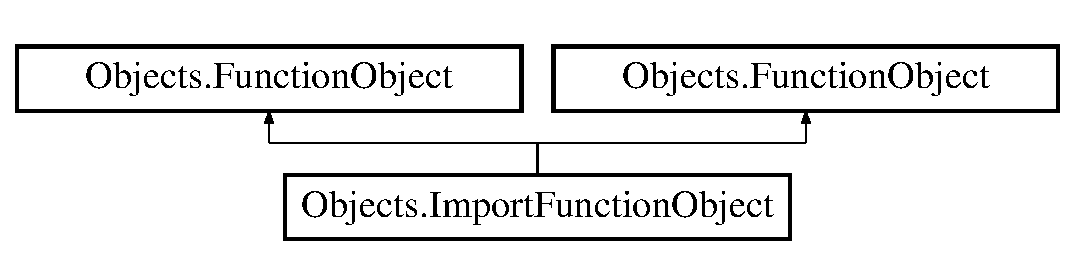
\includegraphics[height=2.000000cm]{class_objects_1_1_import_function_object}
\end{center}
\end{figure}
\subsection*{Public Member Functions}
\begin{DoxyCompactItemize}
\item 
\mbox{\Hypertarget{class_objects_1_1_import_function_object_aab954a59162122dab63b0396346b9de8}\label{class_objects_1_1_import_function_object_aab954a59162122dab63b0396346b9de8}} 
{\bfseries Import\+Function\+Object} (string function\+Name, U\+Int64 base\+Address, string dependency)
\item 
\mbox{\Hypertarget{class_objects_1_1_import_function_object_aab954a59162122dab63b0396346b9de8}\label{class_objects_1_1_import_function_object_aab954a59162122dab63b0396346b9de8}} 
{\bfseries Import\+Function\+Object} (string function\+Name, U\+Int64 base\+Address, string dependency)
\end{DoxyCompactItemize}
\subsection*{Properties}
\begin{DoxyCompactItemize}
\item 
\mbox{\Hypertarget{class_objects_1_1_import_function_object_af58404b027a813c86ca174a3164ca62d}\label{class_objects_1_1_import_function_object_af58404b027a813c86ca174a3164ca62d}} 
U\+Int64 {\bfseries Base\+Address}\hspace{0.3cm}{\ttfamily  \mbox{[}get, set\mbox{]}}
\item 
\mbox{\Hypertarget{class_objects_1_1_import_function_object_acf76bad1d75d6eb65b117d3539279c4b}\label{class_objects_1_1_import_function_object_acf76bad1d75d6eb65b117d3539279c4b}} 
string {\bfseries Dependency}\hspace{0.3cm}{\ttfamily  \mbox{[}get, set\mbox{]}}
\item 
\mbox{\Hypertarget{class_objects_1_1_import_function_object_a0a94ff959aa1e6fd4a7a64ee0936756a}\label{class_objects_1_1_import_function_object_a0a94ff959aa1e6fd4a7a64ee0936756a}} 
List$<$ \mbox{\hyperlink{class_objects_1_1_import_function_object}{Import\+Function\+Object}} $>$ {\bfseries Function\+Object\+List}\hspace{0.3cm}{\ttfamily  \mbox{[}get, set\mbox{]}}
\end{DoxyCompactItemize}


\subsection{Detailed Description}


Definition at line 96 of file I\+P\+C\+Client.\+cs.



The documentation for this class was generated from the following files\+:\begin{DoxyCompactItemize}
\item 
C\+:/\+Users/\+Shehan Vanderputt/\+Downloads/\+Compressed/\+P\+E\+D\+Scanner-\/master/\+P\+E\+D\+Scanner-\/master/\+P\+E\+D\+Scanner\+Lib/\+P\+E\+D\+Scanner\+Lib/I\+P\+C\+Client.\+cs\item 
C\+:/\+Users/\+Shehan Vanderputt/\+Downloads/\+Compressed/\+P\+E\+D\+Scanner-\/master/\+P\+E\+D\+Scanner-\/master/\+Server64\+Bit\+Library/\+Server64\+Bit\+Library/Class1.\+cs\end{DoxyCompactItemize}

\hypertarget{class_class_library_server_1_1_struct_1_1_interop}{}\section{Class\+Library\+Server.\+Struct.\+Interop Class Reference}
\label{class_class_library_server_1_1_struct_1_1_interop}\index{Class\+Library\+Server.\+Struct.\+Interop@{Class\+Library\+Server.\+Struct.\+Interop}}
\subsection*{Public Member Functions}
\begin{DoxyCompactItemize}
\item 
\mbox{\Hypertarget{class_class_library_server_1_1_struct_1_1_interop_a2af7410b79f5980781f65eb4da38af6a}\label{class_class_library_server_1_1_struct_1_1_interop_a2af7410b79f5980781f65eb4da38af6a}} 
static void $\ast$ {\bfseries Get\+Module\+HandleA} (char $\ast$lp\+Module\+Name)
\item 
\mbox{\Hypertarget{class_class_library_server_1_1_struct_1_1_interop_ab10dc5648efa72db11e600a95f20d037}\label{class_class_library_server_1_1_struct_1_1_interop_ab10dc5648efa72db11e600a95f20d037}} 
static void $\ast$ {\bfseries Get\+Module\+HandleW} (char $\ast$lp\+Module\+Name)
\item 
\mbox{\Hypertarget{class_class_library_server_1_1_struct_1_1_interop_a9b4a9685f435e57614a954f94e4115c7}\label{class_class_library_server_1_1_struct_1_1_interop_a9b4a9685f435e57614a954f94e4115c7}} 
static bool {\bfseries Is\+Bad\+Read\+Ptr} (void $\ast$lp\+Base, uint ucb)
\item 
\mbox{\Hypertarget{class_class_library_server_1_1_struct_1_1_interop_a07996454d1197adf9537011fc5cece7a}\label{class_class_library_server_1_1_struct_1_1_interop_a07996454d1197adf9537011fc5cece7a}} 
static bool {\bfseries Is\+Bad\+Read\+Ptr} (void $\ast$lp\+Base, ulong ucb)
\item 
\mbox{\Hypertarget{class_class_library_server_1_1_struct_1_1_interop_a466d767c6d61625fc261d6a06208e303}\label{class_class_library_server_1_1_struct_1_1_interop_a466d767c6d61625fc261d6a06208e303}} 
static void $\ast$ {\bfseries Image\+Directory\+Entry\+To\+Data} (void $\ast$Base, bool Mapped\+As\+Image, ulong Directory\+Entry, out ulong Size)
\item 
\mbox{\Hypertarget{class_class_library_server_1_1_struct_1_1_interop_a1e66c1942db3ffcf045abad0a9118336}\label{class_class_library_server_1_1_struct_1_1_interop_a1e66c1942db3ffcf045abad0a9118336}} 
static void $\ast$ {\bfseries Image\+Directory\+Entry\+To\+Data} (void $\ast$Base, bool Mapped\+As\+Image, ushort Directory\+Entry, out uint Size)
\item 
\mbox{\Hypertarget{class_class_library_server_1_1_struct_1_1_interop_a3bd560e9cad352d3e249482a71928621}\label{class_class_library_server_1_1_struct_1_1_interop_a3bd560e9cad352d3e249482a71928621}} 
static Int\+Ptr {\bfseries Image\+Rva\+To\+Va} (Int\+Ptr p\+Nt\+Headers, Int\+Ptr p\+Base, uint rva, Int\+Ptr p\+Last\+Rva\+Section)
\item 
\mbox{\Hypertarget{class_class_library_server_1_1_struct_1_1_interop_ab56255d4982a9748c444719d10f5219f}\label{class_class_library_server_1_1_struct_1_1_interop_ab56255d4982a9748c444719d10f5219f}} 
static Int\+Ptr {\bfseries Image\+Nt\+Header} (Int\+Ptr p\+Image\+Base)
\item 
\mbox{\Hypertarget{class_class_library_server_1_1_struct_1_1_interop_ac04dbcdb580a0adf5022c702399d8709}\label{class_class_library_server_1_1_struct_1_1_interop_ac04dbcdb580a0adf5022c702399d8709}} 
static bool {\bfseries Map\+And\+Load} (string image\+Name, string dll\+Path, out \mbox{\hyperlink{struct_class_library_server_1_1_struct_1_1_l_o_a_d_e_d___i_m_a_g_e}{L\+O\+A\+D\+E\+D\+\_\+\+I\+M\+A\+GE}} loaded\+Image, bool dot\+Dll, bool read\+Only)
\item 
\mbox{\Hypertarget{class_class_library_server_1_1_struct_1_1_interop_a5e23c3984cc77dd0cd5cd676857e7b38}\label{class_class_library_server_1_1_struct_1_1_interop_a5e23c3984cc77dd0cd5cd676857e7b38}} 
static bool {\bfseries Set\+File\+Pointer\+Ex} (Int\+Ptr h\+File, long li\+Distance\+To\+Move, out long lp\+New\+File\+Pointer, uint dw\+Move\+Method)
\end{DoxyCompactItemize}
\subsection*{Static Public Attributes}
\begin{DoxyCompactItemize}
\item 
\mbox{\Hypertarget{class_class_library_server_1_1_struct_1_1_interop_a1f988dd749571a74a453268b7bd5bb69}\label{class_class_library_server_1_1_struct_1_1_interop_a1f988dd749571a74a453268b7bd5bb69}} 
static readonly ushort {\bfseries I\+M\+A\+G\+E\+\_\+\+D\+I\+R\+E\+C\+T\+O\+R\+Y\+\_\+\+E\+N\+T\+R\+Y\+\_\+\+I\+M\+P\+O\+R\+T32} = 1
\item 
\mbox{\Hypertarget{class_class_library_server_1_1_struct_1_1_interop_aadf1595d26b2ba169c6ae9a91971c844}\label{class_class_library_server_1_1_struct_1_1_interop_aadf1595d26b2ba169c6ae9a91971c844}} 
static readonly ulong {\bfseries I\+M\+A\+G\+E\+\_\+\+D\+I\+R\+E\+C\+T\+O\+R\+Y\+\_\+\+E\+N\+T\+R\+Y\+\_\+\+I\+M\+P\+O\+RT} = 1
\item 
\mbox{\Hypertarget{class_class_library_server_1_1_struct_1_1_interop_a1bacac4010c3c7933c38feddb1108492}\label{class_class_library_server_1_1_struct_1_1_interop_a1bacac4010c3c7933c38feddb1108492}} 
static readonly ushort {\bfseries I\+M\+A\+G\+E\+\_\+\+D\+I\+R\+E\+C\+T\+O\+R\+Y\+\_\+\+E\+N\+T\+R\+Y\+\_\+\+E\+X\+P\+O\+R\+T32} = 0
\item 
\mbox{\Hypertarget{class_class_library_server_1_1_struct_1_1_interop_a26c73da92f92be46d41c15230a75f719}\label{class_class_library_server_1_1_struct_1_1_interop_a26c73da92f92be46d41c15230a75f719}} 
static readonly ulong {\bfseries I\+M\+A\+G\+E\+\_\+\+D\+I\+R\+E\+C\+T\+O\+R\+Y\+\_\+\+E\+N\+T\+R\+Y\+\_\+\+E\+X\+P\+O\+RT} = 0
\end{DoxyCompactItemize}


\subsection{Detailed Description}


Definition at line 340 of file Native\+Dll\+Structure.\+cs.



The documentation for this class was generated from the following file\+:\begin{DoxyCompactItemize}
\item 
C\+:/\+Users/\+Shehan Vanderputt/\+Downloads/\+Compressed/\+P\+E\+D\+Scanner-\/master/\+P\+E\+D\+Scanner-\/master/\+Server64\+Bit\+Library/\+Server64\+Bit\+Library/Native\+Dll\+Structure.\+cs\end{DoxyCompactItemize}

\hypertarget{class_p_e_d_scanner_lib_1_1_struct_1_1_interop}{}\section{P\+E\+D\+Scanner\+Lib.\+Struct.\+Interop Class Reference}
\label{class_p_e_d_scanner_lib_1_1_struct_1_1_interop}\index{P\+E\+D\+Scanner\+Lib.\+Struct.\+Interop@{P\+E\+D\+Scanner\+Lib.\+Struct.\+Interop}}
\subsection*{Public Member Functions}
\begin{DoxyCompactItemize}
\item 
\mbox{\Hypertarget{class_p_e_d_scanner_lib_1_1_struct_1_1_interop_a84a2a6209e0765dc550351642bb9c3d7}\label{class_p_e_d_scanner_lib_1_1_struct_1_1_interop_a84a2a6209e0765dc550351642bb9c3d7}} 
static void $\ast$ {\bfseries Get\+Module\+HandleA} (char $\ast$lp\+Module\+Name)
\item 
\mbox{\Hypertarget{class_p_e_d_scanner_lib_1_1_struct_1_1_interop_a9adb1425939675e4bb2089a3a25132af}\label{class_p_e_d_scanner_lib_1_1_struct_1_1_interop_a9adb1425939675e4bb2089a3a25132af}} 
static void $\ast$ {\bfseries Get\+Module\+HandleW} (char $\ast$lp\+Module\+Name)
\item 
\mbox{\Hypertarget{class_p_e_d_scanner_lib_1_1_struct_1_1_interop_ad51a924319e3af8f37853860f52ded42}\label{class_p_e_d_scanner_lib_1_1_struct_1_1_interop_ad51a924319e3af8f37853860f52ded42}} 
static bool {\bfseries Is\+Bad\+Read\+Ptr} (void $\ast$lp\+Base, uint ucb)
\item 
\mbox{\Hypertarget{class_p_e_d_scanner_lib_1_1_struct_1_1_interop_ad026a33a9699d74f6fe8c7fac1b6d890}\label{class_p_e_d_scanner_lib_1_1_struct_1_1_interop_ad026a33a9699d74f6fe8c7fac1b6d890}} 
static void $\ast$ {\bfseries Image\+Directory\+Entry\+To\+Data} (void $\ast$Base, bool Mapped\+As\+Image, ushort Directory\+Entry, out uint Size)
\item 
\mbox{\Hypertarget{class_p_e_d_scanner_lib_1_1_struct_1_1_interop_a7e67ab62ee7c29cf8940eec1db41fc0f}\label{class_p_e_d_scanner_lib_1_1_struct_1_1_interop_a7e67ab62ee7c29cf8940eec1db41fc0f}} 
static Int\+Ptr {\bfseries Image\+Rva\+To\+Va} (Int\+Ptr p\+Nt\+Headers, Int\+Ptr p\+Base, uint rva, Int\+Ptr p\+Last\+Rva\+Section)
\item 
\mbox{\Hypertarget{class_p_e_d_scanner_lib_1_1_struct_1_1_interop_abf490187652508db85aa44999b0bd032}\label{class_p_e_d_scanner_lib_1_1_struct_1_1_interop_abf490187652508db85aa44999b0bd032}} 
static Int\+Ptr {\bfseries Image\+Nt\+Header} (Int\+Ptr p\+Image\+Base)
\item 
\mbox{\Hypertarget{class_p_e_d_scanner_lib_1_1_struct_1_1_interop_aed20b693f14a56a0723ee148f189c8b2}\label{class_p_e_d_scanner_lib_1_1_struct_1_1_interop_aed20b693f14a56a0723ee148f189c8b2}} 
static bool {\bfseries Map\+And\+Load} (string image\+Name, string dll\+Path, out \mbox{\hyperlink{struct_p_e_d_scanner_lib_1_1_struct_1_1_l_o_a_d_e_d___i_m_a_g_e}{L\+O\+A\+D\+E\+D\+\_\+\+I\+M\+A\+GE}} loaded\+Image, bool dot\+Dll, bool read\+Only)
\item 
\mbox{\Hypertarget{class_p_e_d_scanner_lib_1_1_struct_1_1_interop_acbb75464f4b2f6bc330be350a0ca3264}\label{class_p_e_d_scanner_lib_1_1_struct_1_1_interop_acbb75464f4b2f6bc330be350a0ca3264}} 
static bool {\bfseries Set\+File\+Pointer\+Ex} (Int\+Ptr h\+File, long li\+Distance\+To\+Move, out long lp\+New\+File\+Pointer, uint dw\+Move\+Method)
\end{DoxyCompactItemize}
\subsection*{Static Public Attributes}
\begin{DoxyCompactItemize}
\item 
\mbox{\Hypertarget{class_p_e_d_scanner_lib_1_1_struct_1_1_interop_ada7ee8624dc2e81e32215be6fe93f50d}\label{class_p_e_d_scanner_lib_1_1_struct_1_1_interop_ada7ee8624dc2e81e32215be6fe93f50d}} 
static readonly ushort {\bfseries I\+M\+A\+G\+E\+\_\+\+D\+I\+R\+E\+C\+T\+O\+R\+Y\+\_\+\+E\+N\+T\+R\+Y\+\_\+\+I\+M\+P\+O\+RT} = 1
\item 
\mbox{\Hypertarget{class_p_e_d_scanner_lib_1_1_struct_1_1_interop_ad63757077050d2cb9bb0d4a15e2cf0fb}\label{class_p_e_d_scanner_lib_1_1_struct_1_1_interop_ad63757077050d2cb9bb0d4a15e2cf0fb}} 
static readonly ushort {\bfseries I\+M\+A\+G\+E\+\_\+\+D\+I\+R\+E\+C\+T\+O\+R\+Y\+\_\+\+E\+N\+T\+R\+Y\+\_\+\+E\+X\+P\+O\+RT} = 0
\end{DoxyCompactItemize}


\subsection{Detailed Description}


Definition at line 299 of file Native\+Dll\+Structs.\+cs.



The documentation for this class was generated from the following file\+:\begin{DoxyCompactItemize}
\item 
C\+:/\+Users/\+Shehan Vanderputt/\+Downloads/\+Compressed/\+P\+E\+D\+Scanner-\/master/\+P\+E\+D\+Scanner-\/master/\+P\+E\+D\+Scanner\+Lib/\+P\+E\+D\+Scanner\+Lib/Native\+Dll\+Structs.\+cs\end{DoxyCompactItemize}

\hypertarget{interface_service64_proxy_1_1_i_simple_service64}{}\section{Service64\+Proxy.\+I\+Simple\+Service64 Interface Reference}
\label{interface_service64_proxy_1_1_i_simple_service64}\index{Service64\+Proxy.\+I\+Simple\+Service64@{Service64\+Proxy.\+I\+Simple\+Service64}}
Inheritance diagram for Service64\+Proxy.\+I\+Simple\+Service64\+:\begin{figure}[H]
\begin{center}
\leavevmode
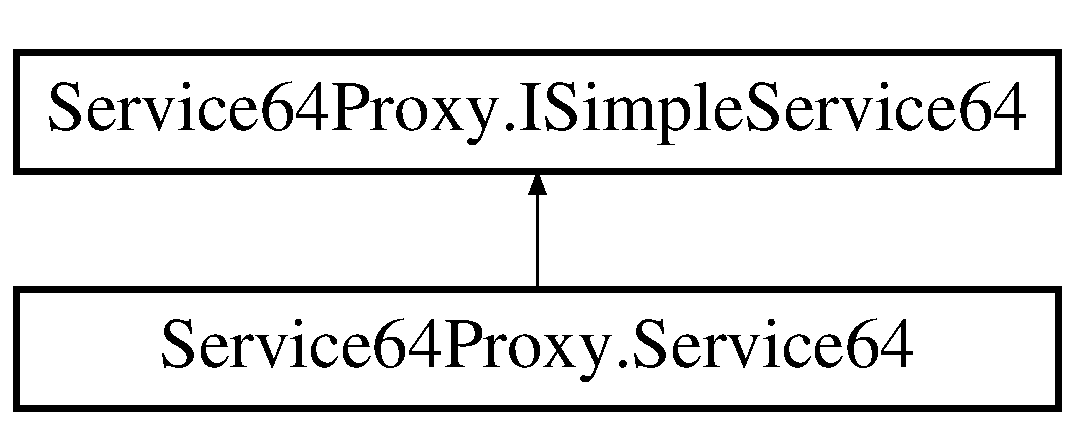
\includegraphics[height=2.000000cm]{interface_service64_proxy_1_1_i_simple_service64}
\end{center}
\end{figure}
\subsection*{Public Member Functions}
\begin{DoxyCompactItemize}
\item 
\mbox{\Hypertarget{interface_service64_proxy_1_1_i_simple_service64_a610966ca798e051a3cfe856f42fc3411}\label{interface_service64_proxy_1_1_i_simple_service64_a610966ca798e051a3cfe856f42fc3411}} 
\mbox{\hyperlink{class_objects_1_1_my_object}{My\+Object}} {\bfseries Load64\+Imports} (\mbox{\hyperlink{class_objects_1_1_my_object}{My\+Object}} my\+Object, string file\+Path, bool mapped\+As\+Image)
\item 
\mbox{\Hypertarget{interface_service64_proxy_1_1_i_simple_service64_a919e029368d2cd30fd1434bd52a1ac83}\label{interface_service64_proxy_1_1_i_simple_service64_a919e029368d2cd30fd1434bd52a1ac83}} 
\mbox{\hyperlink{class_objects_1_1_export_object}{Export\+Object}} {\bfseries Load64\+Exports} (\mbox{\hyperlink{class_objects_1_1_export_object}{Export\+Object}} my\+Object, string file\+Path, bool mapped\+As\+Image)
\end{DoxyCompactItemize}


\subsection{Detailed Description}


Definition at line 13 of file I\+P\+C\+Client.\+cs.



The documentation for this interface was generated from the following file\+:\begin{DoxyCompactItemize}
\item 
C\+:/\+Users/\+Shehan Vanderputt/\+Downloads/\+Compressed/\+P\+E\+D\+Scanner-\/master/\+P\+E\+D\+Scanner-\/master/\+P\+E\+D\+Scanner\+Lib/\+P\+E\+D\+Scanner\+Lib/I\+P\+C\+Client.\+cs\end{DoxyCompactItemize}

\hypertarget{interface_server64_1_1_i_simple_service64}{}\section{Server64.\+I\+Simple\+Service64 Interface Reference}
\label{interface_server64_1_1_i_simple_service64}\index{Server64.\+I\+Simple\+Service64@{Server64.\+I\+Simple\+Service64}}
Inheritance diagram for Server64.\+I\+Simple\+Service64\+:\begin{figure}[H]
\begin{center}
\leavevmode
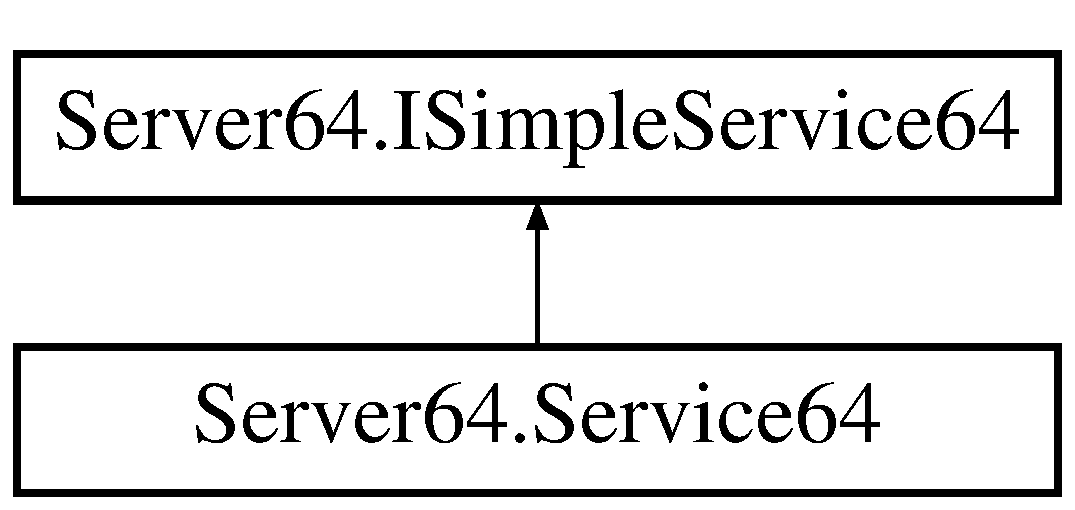
\includegraphics[height=2.000000cm]{interface_server64_1_1_i_simple_service64}
\end{center}
\end{figure}
\subsection*{Public Member Functions}
\begin{DoxyCompactItemize}
\item 
\mbox{\Hypertarget{interface_server64_1_1_i_simple_service64_aeca689c70d6ab240e8016077d12da6c4}\label{interface_server64_1_1_i_simple_service64_aeca689c70d6ab240e8016077d12da6c4}} 
\mbox{\hyperlink{class_objects_1_1_export_object}{Export\+Object}} {\bfseries Load64\+Exports} (\mbox{\hyperlink{class_objects_1_1_export_object}{Export\+Object}} my\+Object, string file\+Path, bool mapped\+As\+Image)
\item 
\mbox{\Hypertarget{interface_server64_1_1_i_simple_service64_af11082acc79a1408f29a0d81fcaafe0c}\label{interface_server64_1_1_i_simple_service64_af11082acc79a1408f29a0d81fcaafe0c}} 
\mbox{\hyperlink{class_objects_1_1_my_object}{My\+Object}} {\bfseries Load64\+Imports} (\mbox{\hyperlink{class_objects_1_1_my_object}{My\+Object}} my\+Object, string file\+Path, bool mapped\+As\+Image)
\end{DoxyCompactItemize}


\subsection{Detailed Description}


Definition at line 86 of file Class1.\+cs.



The documentation for this interface was generated from the following file\+:\begin{DoxyCompactItemize}
\item 
C\+:/\+Users/\+Shehan Vanderputt/\+Downloads/\+Compressed/\+P\+E\+D\+Scanner-\/master/\+P\+E\+D\+Scanner-\/master/\+Server64\+Bit\+Library/\+Server64\+Bit\+Library/Class1.\+cs\end{DoxyCompactItemize}

\hypertarget{struct_p_e_d_scanner_lib_1_1_struct_1_1_l_o_a_d_e_d___i_m_a_g_e}{}\section{P\+E\+D\+Scanner\+Lib.\+Struct.\+L\+O\+A\+D\+E\+D\+\_\+\+I\+M\+A\+GE Struct Reference}
\label{struct_p_e_d_scanner_lib_1_1_struct_1_1_l_o_a_d_e_d___i_m_a_g_e}\index{P\+E\+D\+Scanner\+Lib.\+Struct.\+L\+O\+A\+D\+E\+D\+\_\+\+I\+M\+A\+GE@{P\+E\+D\+Scanner\+Lib.\+Struct.\+L\+O\+A\+D\+E\+D\+\_\+\+I\+M\+A\+GE}}
\subsection*{Public Attributes}
\begin{DoxyCompactItemize}
\item 
\mbox{\Hypertarget{struct_p_e_d_scanner_lib_1_1_struct_1_1_l_o_a_d_e_d___i_m_a_g_e_a0690fe627a98cb55be3f9a089eb2dc5b}\label{struct_p_e_d_scanner_lib_1_1_struct_1_1_l_o_a_d_e_d___i_m_a_g_e_a0690fe627a98cb55be3f9a089eb2dc5b}} 
Int\+Ptr {\bfseries module\+Name}
\item 
\mbox{\Hypertarget{struct_p_e_d_scanner_lib_1_1_struct_1_1_l_o_a_d_e_d___i_m_a_g_e_a318a872738142ed86ca5072df21418c8}\label{struct_p_e_d_scanner_lib_1_1_struct_1_1_l_o_a_d_e_d___i_m_a_g_e_a318a872738142ed86ca5072df21418c8}} 
Int\+Ptr {\bfseries h\+File}
\item 
\mbox{\Hypertarget{struct_p_e_d_scanner_lib_1_1_struct_1_1_l_o_a_d_e_d___i_m_a_g_e_acd98f03c4c6f4e3b3dc6ee873c046e3c}\label{struct_p_e_d_scanner_lib_1_1_struct_1_1_l_o_a_d_e_d___i_m_a_g_e_acd98f03c4c6f4e3b3dc6ee873c046e3c}} 
Int\+Ptr {\bfseries Mapped\+Address}
\item 
\mbox{\Hypertarget{struct_p_e_d_scanner_lib_1_1_struct_1_1_l_o_a_d_e_d___i_m_a_g_e_af4885f7e707ae785910014e133d1b48f}\label{struct_p_e_d_scanner_lib_1_1_struct_1_1_l_o_a_d_e_d___i_m_a_g_e_af4885f7e707ae785910014e133d1b48f}} 
Int\+Ptr {\bfseries File\+Header}
\item 
\mbox{\Hypertarget{struct_p_e_d_scanner_lib_1_1_struct_1_1_l_o_a_d_e_d___i_m_a_g_e_a1dc0f5d821c8e9b164636a144cf43a99}\label{struct_p_e_d_scanner_lib_1_1_struct_1_1_l_o_a_d_e_d___i_m_a_g_e_a1dc0f5d821c8e9b164636a144cf43a99}} 
Int\+Ptr {\bfseries last\+Rva\+Section}
\item 
\mbox{\Hypertarget{struct_p_e_d_scanner_lib_1_1_struct_1_1_l_o_a_d_e_d___i_m_a_g_e_a785be5a7f68c095810fb9115e8da60b4}\label{struct_p_e_d_scanner_lib_1_1_struct_1_1_l_o_a_d_e_d___i_m_a_g_e_a785be5a7f68c095810fb9115e8da60b4}} 
U\+Int32 {\bfseries numb\+Of\+Sections}
\item 
\mbox{\Hypertarget{struct_p_e_d_scanner_lib_1_1_struct_1_1_l_o_a_d_e_d___i_m_a_g_e_ae78d0cec26e86b86b23d0789fc5b972c}\label{struct_p_e_d_scanner_lib_1_1_struct_1_1_l_o_a_d_e_d___i_m_a_g_e_ae78d0cec26e86b86b23d0789fc5b972c}} 
Int\+Ptr {\bfseries first\+Rva\+Section}
\item 
\mbox{\Hypertarget{struct_p_e_d_scanner_lib_1_1_struct_1_1_l_o_a_d_e_d___i_m_a_g_e_a4987f9c76edb26caa296364b97c16557}\label{struct_p_e_d_scanner_lib_1_1_struct_1_1_l_o_a_d_e_d___i_m_a_g_e_a4987f9c76edb26caa296364b97c16557}} 
U\+Int32 {\bfseries charachteristics}
\item 
\mbox{\Hypertarget{struct_p_e_d_scanner_lib_1_1_struct_1_1_l_o_a_d_e_d___i_m_a_g_e_aea3674d29dd7b431461292714cb981c7}\label{struct_p_e_d_scanner_lib_1_1_struct_1_1_l_o_a_d_e_d___i_m_a_g_e_aea3674d29dd7b431461292714cb981c7}} 
ushort {\bfseries system\+Image}
\item 
\mbox{\Hypertarget{struct_p_e_d_scanner_lib_1_1_struct_1_1_l_o_a_d_e_d___i_m_a_g_e_aa1d57df52b2d71437cc21983ecc01835}\label{struct_p_e_d_scanner_lib_1_1_struct_1_1_l_o_a_d_e_d___i_m_a_g_e_aa1d57df52b2d71437cc21983ecc01835}} 
ushort {\bfseries dos\+Image}
\item 
\mbox{\Hypertarget{struct_p_e_d_scanner_lib_1_1_struct_1_1_l_o_a_d_e_d___i_m_a_g_e_a8b229875251d9842df012bf1f6454bd8}\label{struct_p_e_d_scanner_lib_1_1_struct_1_1_l_o_a_d_e_d___i_m_a_g_e_a8b229875251d9842df012bf1f6454bd8}} 
ushort {\bfseries read\+Only}
\item 
\mbox{\Hypertarget{struct_p_e_d_scanner_lib_1_1_struct_1_1_l_o_a_d_e_d___i_m_a_g_e_a81cad340f314f1dead0c855ef84f5c13}\label{struct_p_e_d_scanner_lib_1_1_struct_1_1_l_o_a_d_e_d___i_m_a_g_e_a81cad340f314f1dead0c855ef84f5c13}} 
ushort {\bfseries version}
\item 
\mbox{\Hypertarget{struct_p_e_d_scanner_lib_1_1_struct_1_1_l_o_a_d_e_d___i_m_a_g_e_a3ddbb82db8b3baab75da6fd7e28220bc}\label{struct_p_e_d_scanner_lib_1_1_struct_1_1_l_o_a_d_e_d___i_m_a_g_e_a3ddbb82db8b3baab75da6fd7e28220bc}} 
Int\+Ptr {\bfseries links\+\_\+1}
\item 
\mbox{\Hypertarget{struct_p_e_d_scanner_lib_1_1_struct_1_1_l_o_a_d_e_d___i_m_a_g_e_a2d9e10b706c35c2b4702697ebb62478a}\label{struct_p_e_d_scanner_lib_1_1_struct_1_1_l_o_a_d_e_d___i_m_a_g_e_a2d9e10b706c35c2b4702697ebb62478a}} 
Int\+Ptr {\bfseries links\+\_\+2}
\item 
\mbox{\Hypertarget{struct_p_e_d_scanner_lib_1_1_struct_1_1_l_o_a_d_e_d___i_m_a_g_e_a6d4a58f81477494094f0d6a2c20377b5}\label{struct_p_e_d_scanner_lib_1_1_struct_1_1_l_o_a_d_e_d___i_m_a_g_e_a6d4a58f81477494094f0d6a2c20377b5}} 
U\+Int32 {\bfseries size\+Of\+Image}
\end{DoxyCompactItemize}


\subsection{Detailed Description}


Definition at line 269 of file Native\+Dll\+Structs.\+cs.



The documentation for this struct was generated from the following file\+:\begin{DoxyCompactItemize}
\item 
C\+:/\+Users/\+Shehan Vanderputt/\+Downloads/\+Compressed/\+P\+E\+D\+Scanner-\/master/\+P\+E\+D\+Scanner-\/master/\+P\+E\+D\+Scanner\+Lib/\+P\+E\+D\+Scanner\+Lib/Native\+Dll\+Structs.\+cs\end{DoxyCompactItemize}

\hypertarget{struct_class_library_server_1_1_struct_1_1_l_o_a_d_e_d___i_m_a_g_e}{}\section{Class\+Library\+Server.\+Struct.\+L\+O\+A\+D\+E\+D\+\_\+\+I\+M\+A\+GE Struct Reference}
\label{struct_class_library_server_1_1_struct_1_1_l_o_a_d_e_d___i_m_a_g_e}\index{Class\+Library\+Server.\+Struct.\+L\+O\+A\+D\+E\+D\+\_\+\+I\+M\+A\+GE@{Class\+Library\+Server.\+Struct.\+L\+O\+A\+D\+E\+D\+\_\+\+I\+M\+A\+GE}}
\subsection*{Public Attributes}
\begin{DoxyCompactItemize}
\item 
\mbox{\Hypertarget{struct_class_library_server_1_1_struct_1_1_l_o_a_d_e_d___i_m_a_g_e_a3faa9b3b0f2efa60ec456195f9b77e09}\label{struct_class_library_server_1_1_struct_1_1_l_o_a_d_e_d___i_m_a_g_e_a3faa9b3b0f2efa60ec456195f9b77e09}} 
Int\+Ptr {\bfseries module\+Name}
\item 
\mbox{\Hypertarget{struct_class_library_server_1_1_struct_1_1_l_o_a_d_e_d___i_m_a_g_e_af1430aa11720ab56718d245148c52f54}\label{struct_class_library_server_1_1_struct_1_1_l_o_a_d_e_d___i_m_a_g_e_af1430aa11720ab56718d245148c52f54}} 
Int\+Ptr {\bfseries h\+File}
\item 
\mbox{\Hypertarget{struct_class_library_server_1_1_struct_1_1_l_o_a_d_e_d___i_m_a_g_e_aa1ca7820df06c78b5f5041f8865584ff}\label{struct_class_library_server_1_1_struct_1_1_l_o_a_d_e_d___i_m_a_g_e_aa1ca7820df06c78b5f5041f8865584ff}} 
Int\+Ptr {\bfseries Mapped\+Address}
\item 
\mbox{\Hypertarget{struct_class_library_server_1_1_struct_1_1_l_o_a_d_e_d___i_m_a_g_e_a75834c127ac8c2c5e856b0249a92fd9a}\label{struct_class_library_server_1_1_struct_1_1_l_o_a_d_e_d___i_m_a_g_e_a75834c127ac8c2c5e856b0249a92fd9a}} 
Int\+Ptr {\bfseries File\+Header}
\item 
\mbox{\Hypertarget{struct_class_library_server_1_1_struct_1_1_l_o_a_d_e_d___i_m_a_g_e_ae2b986ddcf4c7e68fd2cfa7e4f9f07f7}\label{struct_class_library_server_1_1_struct_1_1_l_o_a_d_e_d___i_m_a_g_e_ae2b986ddcf4c7e68fd2cfa7e4f9f07f7}} 
Int\+Ptr {\bfseries last\+Rva\+Section}
\item 
\mbox{\Hypertarget{struct_class_library_server_1_1_struct_1_1_l_o_a_d_e_d___i_m_a_g_e_a8e02b715a27dbd6397b807e671e7dce6}\label{struct_class_library_server_1_1_struct_1_1_l_o_a_d_e_d___i_m_a_g_e_a8e02b715a27dbd6397b807e671e7dce6}} 
U\+Int32 {\bfseries numb\+Of\+Sections}
\item 
\mbox{\Hypertarget{struct_class_library_server_1_1_struct_1_1_l_o_a_d_e_d___i_m_a_g_e_ac2c2494f4843069499b2206399453b44}\label{struct_class_library_server_1_1_struct_1_1_l_o_a_d_e_d___i_m_a_g_e_ac2c2494f4843069499b2206399453b44}} 
Int\+Ptr {\bfseries first\+Rva\+Section}
\item 
\mbox{\Hypertarget{struct_class_library_server_1_1_struct_1_1_l_o_a_d_e_d___i_m_a_g_e_a3ed477e0036952e4903561c4d06668c7}\label{struct_class_library_server_1_1_struct_1_1_l_o_a_d_e_d___i_m_a_g_e_a3ed477e0036952e4903561c4d06668c7}} 
U\+Int32 {\bfseries charachteristics}
\item 
\mbox{\Hypertarget{struct_class_library_server_1_1_struct_1_1_l_o_a_d_e_d___i_m_a_g_e_af0d371a9a43d7c1ec04635d62de5afb0}\label{struct_class_library_server_1_1_struct_1_1_l_o_a_d_e_d___i_m_a_g_e_af0d371a9a43d7c1ec04635d62de5afb0}} 
ushort {\bfseries system\+Image}
\item 
\mbox{\Hypertarget{struct_class_library_server_1_1_struct_1_1_l_o_a_d_e_d___i_m_a_g_e_ac3a9f5f597f46f8f61ce8923954badfa}\label{struct_class_library_server_1_1_struct_1_1_l_o_a_d_e_d___i_m_a_g_e_ac3a9f5f597f46f8f61ce8923954badfa}} 
ushort {\bfseries dos\+Image}
\item 
\mbox{\Hypertarget{struct_class_library_server_1_1_struct_1_1_l_o_a_d_e_d___i_m_a_g_e_af43739f726ac055837e4543a4992dea8}\label{struct_class_library_server_1_1_struct_1_1_l_o_a_d_e_d___i_m_a_g_e_af43739f726ac055837e4543a4992dea8}} 
ushort {\bfseries read\+Only}
\item 
\mbox{\Hypertarget{struct_class_library_server_1_1_struct_1_1_l_o_a_d_e_d___i_m_a_g_e_a03ae8c11ad7638771ddaeec473f3ab52}\label{struct_class_library_server_1_1_struct_1_1_l_o_a_d_e_d___i_m_a_g_e_a03ae8c11ad7638771ddaeec473f3ab52}} 
ushort {\bfseries version}
\item 
\mbox{\Hypertarget{struct_class_library_server_1_1_struct_1_1_l_o_a_d_e_d___i_m_a_g_e_aa7c4bc4d7dc32c378e3cead683db6972}\label{struct_class_library_server_1_1_struct_1_1_l_o_a_d_e_d___i_m_a_g_e_aa7c4bc4d7dc32c378e3cead683db6972}} 
Int\+Ptr {\bfseries links\+\_\+1}
\item 
\mbox{\Hypertarget{struct_class_library_server_1_1_struct_1_1_l_o_a_d_e_d___i_m_a_g_e_af1907b2486865c55e89ad24c0745ddb5}\label{struct_class_library_server_1_1_struct_1_1_l_o_a_d_e_d___i_m_a_g_e_af1907b2486865c55e89ad24c0745ddb5}} 
Int\+Ptr {\bfseries links\+\_\+2}
\item 
\mbox{\Hypertarget{struct_class_library_server_1_1_struct_1_1_l_o_a_d_e_d___i_m_a_g_e_ad26930165f7fd02bdf50fdfd54932a09}\label{struct_class_library_server_1_1_struct_1_1_l_o_a_d_e_d___i_m_a_g_e_ad26930165f7fd02bdf50fdfd54932a09}} 
U\+Int32 {\bfseries size\+Of\+Image}
\end{DoxyCompactItemize}


\subsection{Detailed Description}


Definition at line 310 of file Native\+Dll\+Structure.\+cs.



The documentation for this struct was generated from the following file\+:\begin{DoxyCompactItemize}
\item 
C\+:/\+Users/\+Shehan Vanderputt/\+Downloads/\+Compressed/\+P\+E\+D\+Scanner-\/master/\+P\+E\+D\+Scanner-\/master/\+Server64\+Bit\+Library/\+Server64\+Bit\+Library/Native\+Dll\+Structure.\+cs\end{DoxyCompactItemize}

\hypertarget{class_p_e_scanner_1_1_main_window}{}\section{P\+E\+Scanner.\+Main\+Window Class Reference}
\label{class_p_e_scanner_1_1_main_window}\index{P\+E\+Scanner.\+Main\+Window@{P\+E\+Scanner.\+Main\+Window}}
Inheritance diagram for P\+E\+Scanner.\+Main\+Window\+:\begin{figure}[H]
\begin{center}
\leavevmode
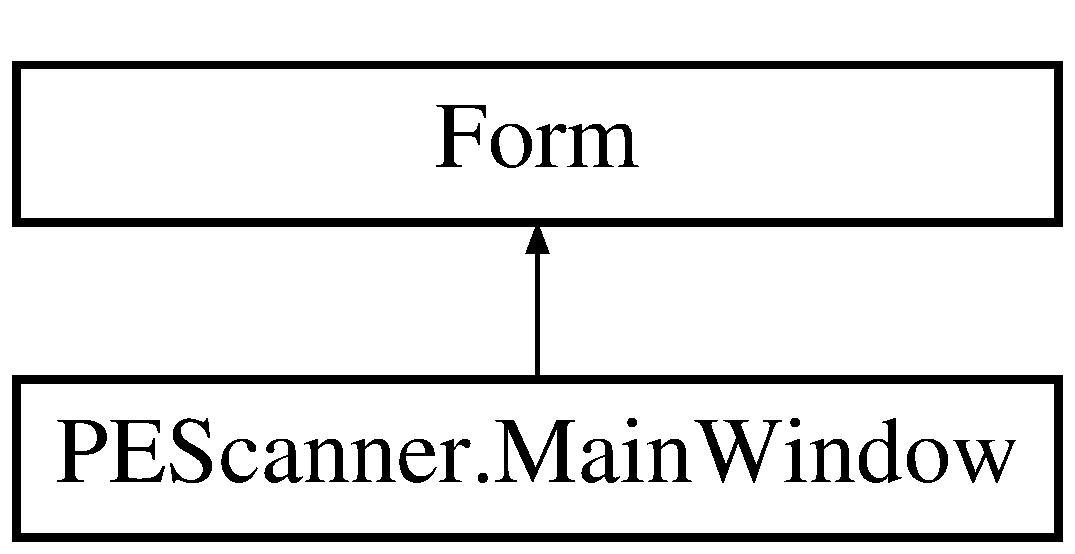
\includegraphics[height=2.000000cm]{class_p_e_scanner_1_1_main_window}
\end{center}
\end{figure}
\subsection*{Public Member Functions}
\begin{DoxyCompactItemize}
\item 
\mbox{\Hypertarget{class_p_e_scanner_1_1_main_window_a1008845c06974fcef59ed792b2cf2532}\label{class_p_e_scanner_1_1_main_window_a1008845c06974fcef59ed792b2cf2532}} 
{\bfseries Main\+Window} (String file\+Path)
\item 
\mbox{\Hypertarget{class_p_e_scanner_1_1_main_window_a2a61549f3aa9dbf1ad31c1a7f0ee7f25}\label{class_p_e_scanner_1_1_main_window_a2a61549f3aa9dbf1ad31c1a7f0ee7f25}} 
{\bfseries Main\+Window} (\mbox{\hyperlink{class_p_e_d_scanner_lib_1_1_core_1_1_portable_executable}{Portable\+Executable}} portable\+Executable)
\end{DoxyCompactItemize}
\subsection*{Public Attributes}
\begin{DoxyCompactItemize}
\item 
\mbox{\Hypertarget{class_p_e_scanner_1_1_main_window_a8ee987dc041e039082488af2717b45fc}\label{class_p_e_scanner_1_1_main_window_a8ee987dc041e039082488af2717b45fc}} 
List$<$ string $>$ {\bfseries list\+Of\+Branch}
\end{DoxyCompactItemize}
\subsection*{Protected Member Functions}
\begin{DoxyCompactItemize}
\item 
\mbox{\Hypertarget{class_p_e_scanner_1_1_main_window_a032cf4c0426b6781bd436bb3dc1c254d}\label{class_p_e_scanner_1_1_main_window_a032cf4c0426b6781bd436bb3dc1c254d}} 
void {\bfseries tree\+View\+Dependencies\+\_\+\+After\+Select} (object sender, System.\+Windows.\+Forms.\+Tree\+View\+Event\+Args e)
\item 
override void \mbox{\hyperlink{class_p_e_scanner_1_1_main_window_a9e2a0de6cb116253b2e7bb35da115ed9}{Dispose}} (bool disposing)
\begin{DoxyCompactList}\small\item\em Clean up any resources being used. \end{DoxyCompactList}\end{DoxyCompactItemize}


\subsection{Detailed Description}


Definition at line 13 of file Main\+Window.\+cs.



\subsection{Member Function Documentation}
\mbox{\Hypertarget{class_p_e_scanner_1_1_main_window_a9e2a0de6cb116253b2e7bb35da115ed9}\label{class_p_e_scanner_1_1_main_window_a9e2a0de6cb116253b2e7bb35da115ed9}} 
\index{P\+E\+Scanner\+::\+Main\+Window@{P\+E\+Scanner\+::\+Main\+Window}!Dispose@{Dispose}}
\index{Dispose@{Dispose}!P\+E\+Scanner\+::\+Main\+Window@{P\+E\+Scanner\+::\+Main\+Window}}
\subsubsection{\texorpdfstring{Dispose()}{Dispose()}}
{\footnotesize\ttfamily override void P\+E\+Scanner.\+Main\+Window.\+Dispose (\begin{DoxyParamCaption}\item[{bool}]{disposing }\end{DoxyParamCaption})\hspace{0.3cm}{\ttfamily [protected]}}



Clean up any resources being used. 


\begin{DoxyParams}{Parameters}
{\em disposing} & true if managed resources should be disposed; otherwise, false.\\
\hline
\end{DoxyParams}


Definition at line 14 of file Main\+Window.\+Designer.\+cs.



The documentation for this class was generated from the following files\+:\begin{DoxyCompactItemize}
\item 
C\+:/\+Users/\+Shehan Vanderputt/\+Downloads/\+Compressed/\+P\+E\+D\+Scanner-\/master/\+P\+E\+D\+Scanner-\/master/\+P\+E\+D\+Scanner\+G\+U\+I/\+P\+E\+Scanner/Main\+Window.\+cs\item 
C\+:/\+Users/\+Shehan Vanderputt/\+Downloads/\+Compressed/\+P\+E\+D\+Scanner-\/master/\+P\+E\+D\+Scanner-\/master/\+P\+E\+D\+Scanner\+G\+U\+I/\+P\+E\+Scanner/Main\+Window.\+Designer.\+cs\end{DoxyCompactItemize}

\hypertarget{class_wizard_1_1_main_window}{}\section{Wizard.\+Main\+Window Class Reference}
\label{class_wizard_1_1_main_window}\index{Wizard.\+Main\+Window@{Wizard.\+Main\+Window}}


Interaction logic for Main\+Window.\+xaml  


Inheritance diagram for Wizard.\+Main\+Window\+:\begin{figure}[H]
\begin{center}
\leavevmode
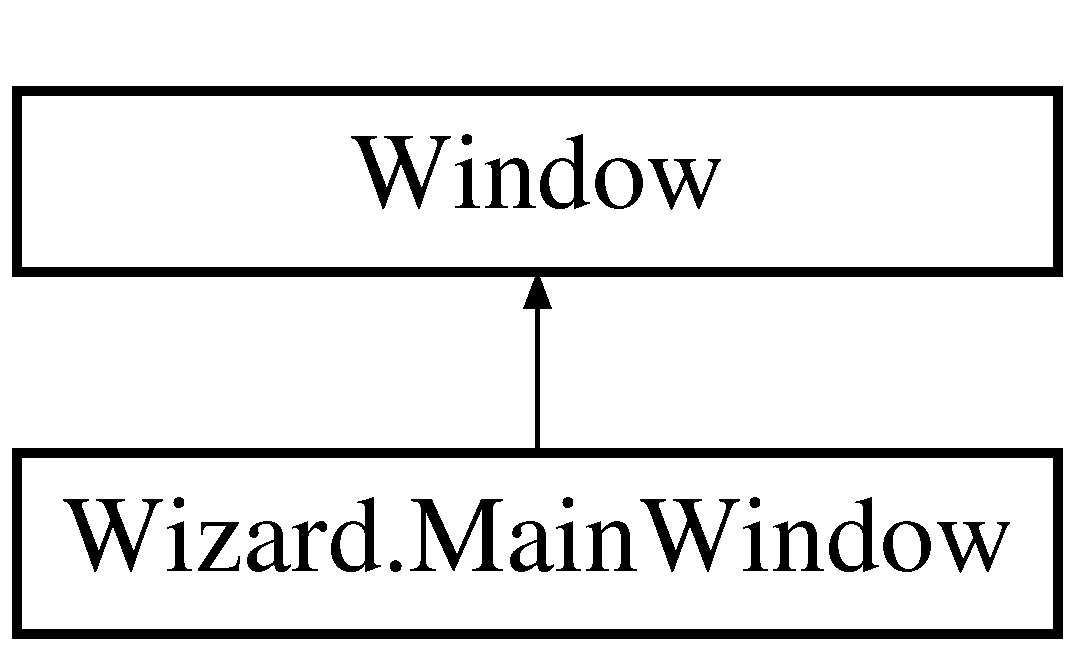
\includegraphics[height=2.000000cm]{class_wizard_1_1_main_window}
\end{center}
\end{figure}
\subsection*{Public Member Functions}
\begin{DoxyCompactItemize}
\item 
\mbox{\Hypertarget{class_wizard_1_1_main_window_ad88b092b55742a7c3ab9f24acdc84f70}\label{class_wizard_1_1_main_window_ad88b092b55742a7c3ab9f24acdc84f70}} 
{\bfseries Main\+Window} (String file\+Path)
\item 
\mbox{\Hypertarget{class_wizard_1_1_main_window_a049459edae54d9aff0ece0fbf9431a35}\label{class_wizard_1_1_main_window_a049459edae54d9aff0ece0fbf9431a35}} 
{\bfseries Main\+Window} (\mbox{\hyperlink{class_p_e_d_scanner_lib_1_1_core_1_1_portable_executable}{Portable\+Executable}} portable\+Executable)
\item 
\mbox{\Hypertarget{class_wizard_1_1_main_window_ae8d6062a995d86d235408f051ff48bfb}\label{class_wizard_1_1_main_window_ae8d6062a995d86d235408f051ff48bfb}} 
void {\bfseries Tree\+View\+Item\+\_\+\+Expanded} (object sender, Routed\+Event\+Args e)
\item 
\mbox{\Hypertarget{class_wizard_1_1_main_window_a4ab7c3c6ceb6642c122dd0c32a65c2f6}\label{class_wizard_1_1_main_window_a4ab7c3c6ceb6642c122dd0c32a65c2f6}} 
void {\bfseries Populate\+Imports} (List$<$ \mbox{\hyperlink{class_objects_1_1_import_function_object}{Import\+Function\+Object}} $>$ imports)
\item 
\mbox{\Hypertarget{class_wizard_1_1_main_window_a4420d6f60644433b6bba116896125f55}\label{class_wizard_1_1_main_window_a4420d6f60644433b6bba116896125f55}} 
void {\bfseries Populate\+Exports} (List$<$ \mbox{\hyperlink{class_objects_1_1_function_object}{Function\+Object}} $>$ exports)
\item 
\mbox{\Hypertarget{class_wizard_1_1_main_window_ac3a622330963376c3f4219bb5cdda623}\label{class_wizard_1_1_main_window_ac3a622330963376c3f4219bb5cdda623}} 
void {\bfseries Populate\+Headers} (List$<$ \mbox{\hyperlink{class_p_e_d_scanner_lib_1_1_objects_1_1_header_object}{Header\+Object}} $>$ headers)
\end{DoxyCompactItemize}
\subsection*{Protected Member Functions}
\begin{DoxyCompactItemize}
\item 
\mbox{\Hypertarget{class_wizard_1_1_main_window_a8f24447d5aca177216cbff16a84aa14d}\label{class_wizard_1_1_main_window_a8f24447d5aca177216cbff16a84aa14d}} 
void {\bfseries tree\+View\+Dependencies\+\_\+\+After\+Select} (object sender, Routed\+Event\+Args e)
\end{DoxyCompactItemize}


\subsection{Detailed Description}
Interaction logic for Main\+Window.\+xaml 



Definition at line 22 of file Main\+Window.\+xaml.\+cs.



The documentation for this class was generated from the following file\+:\begin{DoxyCompactItemize}
\item 
C\+:/\+Users/\+Shehan Vanderputt/\+Downloads/\+Compressed/\+P\+E\+D\+Scanner-\/master/\+P\+E\+D\+Scanner-\/master/\+P\+E\+D\+Scanner\+G\+U\+I\+W\+P\+F/\+P\+E\+D\+Scanner/\+P\+E\+D\+Scanner/Main\+Window.\+xaml.\+cs\end{DoxyCompactItemize}

\hypertarget{class_objects_1_1_my_object}{}\section{Objects.\+My\+Object Class Reference}
\label{class_objects_1_1_my_object}\index{Objects.\+My\+Object@{Objects.\+My\+Object}}
\subsection*{Public Member Functions}
\begin{DoxyCompactItemize}
\item 
\mbox{\Hypertarget{class_objects_1_1_my_object_a3b745d678a467607738e0a4b5d677e44}\label{class_objects_1_1_my_object_a3b745d678a467607738e0a4b5d677e44}} 
{\bfseries My\+Object} (List$<$ \mbox{\hyperlink{class_objects_1_1_import_function_object}{Import\+Function\+Object}} $>$ list)
\item 
\mbox{\Hypertarget{class_objects_1_1_my_object_a3b745d678a467607738e0a4b5d677e44}\label{class_objects_1_1_my_object_a3b745d678a467607738e0a4b5d677e44}} 
{\bfseries My\+Object} (List$<$ \mbox{\hyperlink{class_objects_1_1_import_function_object}{Import\+Function\+Object}} $>$ list)
\end{DoxyCompactItemize}
\subsection*{Properties}
\begin{DoxyCompactItemize}
\item 
\mbox{\Hypertarget{class_objects_1_1_my_object_a0af5a42cf0a47c368cd6a39bb3d6dcc8}\label{class_objects_1_1_my_object_a0af5a42cf0a47c368cd6a39bb3d6dcc8}} 
List$<$ \mbox{\hyperlink{class_objects_1_1_import_function_object}{Import\+Function\+Object}} $>$ {\bfseries Function\+Object\+List}\hspace{0.3cm}{\ttfamily  \mbox{[}get, set\mbox{]}}
\end{DoxyCompactItemize}


\subsection{Detailed Description}


Definition at line 63 of file I\+P\+C\+Client.\+cs.



The documentation for this class was generated from the following files\+:\begin{DoxyCompactItemize}
\item 
C\+:/\+Users/\+Shehan Vanderputt/\+Downloads/\+Compressed/\+P\+E\+D\+Scanner-\/master/\+P\+E\+D\+Scanner-\/master/\+P\+E\+D\+Scanner\+Lib/\+P\+E\+D\+Scanner\+Lib/I\+P\+C\+Client.\+cs\item 
C\+:/\+Users/\+Shehan Vanderputt/\+Downloads/\+Compressed/\+P\+E\+D\+Scanner-\/master/\+P\+E\+D\+Scanner-\/master/\+Server64\+Bit\+Library/\+Server64\+Bit\+Library/Class1.\+cs\end{DoxyCompactItemize}

\hypertarget{class_server64_1_1_my_server}{}\section{Server64.\+My\+Server Class Reference}
\label{class_server64_1_1_my_server}\index{Server64.\+My\+Server@{Server64.\+My\+Server}}
\subsection*{Public Member Functions}
\begin{DoxyCompactItemize}
\item 
\mbox{\Hypertarget{class_server64_1_1_my_server_ab3bf5d76d07698a64cd2edfd4a541ddb}\label{class_server64_1_1_my_server_ab3bf5d76d07698a64cd2edfd4a541ddb}} 
void {\bfseries Server} ()
\end{DoxyCompactItemize}


\subsection{Detailed Description}


Definition at line 242 of file Class1.\+cs.



The documentation for this class was generated from the following file\+:\begin{DoxyCompactItemize}
\item 
C\+:/\+Users/\+Shehan Vanderputt/\+Downloads/\+Compressed/\+P\+E\+D\+Scanner-\/master/\+P\+E\+D\+Scanner-\/master/\+Server64\+Bit\+Library/\+Server64\+Bit\+Library/Class1.\+cs\end{DoxyCompactItemize}

\hypertarget{class_wizard_1_1_page_function_display_reverse_dependencies}{}\section{Wizard.\+Page\+Function\+Display\+Reverse\+Dependencies Class Reference}
\label{class_wizard_1_1_page_function_display_reverse_dependencies}\index{Wizard.\+Page\+Function\+Display\+Reverse\+Dependencies@{Wizard.\+Page\+Function\+Display\+Reverse\+Dependencies}}


Interaction logic for Page\+Function\+Display\+Reverse\+Dependencies.\+xaml  


Inheritance diagram for Wizard.\+Page\+Function\+Display\+Reverse\+Dependencies\+:\begin{figure}[H]
\begin{center}
\leavevmode
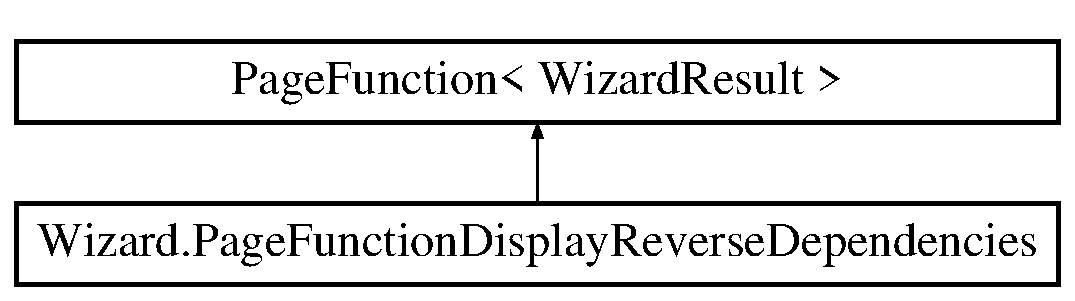
\includegraphics[height=2.000000cm]{class_wizard_1_1_page_function_display_reverse_dependencies}
\end{center}
\end{figure}
\subsection*{Public Member Functions}
\begin{DoxyCompactItemize}
\item 
\mbox{\Hypertarget{class_wizard_1_1_page_function_display_reverse_dependencies_a0e704879bfa179c39d73759727fdc6be}\label{class_wizard_1_1_page_function_display_reverse_dependencies_a0e704879bfa179c39d73759727fdc6be}} 
{\bfseries Page\+Function\+Display\+Reverse\+Dependencies} (\mbox{\hyperlink{class_wizard_1_1_wizard_data}{Wizard\+Data}} wizard\+Data)
\end{DoxyCompactItemize}


\subsection{Detailed Description}
Interaction logic for Page\+Function\+Display\+Reverse\+Dependencies.\+xaml 



Definition at line 22 of file Page\+Function\+Display\+Reverse\+Dependencies.\+xaml.\+cs.



The documentation for this class was generated from the following file\+:\begin{DoxyCompactItemize}
\item 
C\+:/\+Users/\+Shehan Vanderputt/\+Downloads/\+Compressed/\+P\+E\+D\+Scanner-\/master/\+P\+E\+D\+Scanner-\/master/\+P\+E\+D\+Scanner\+G\+U\+I\+W\+P\+F/\+P\+E\+D\+Scanner/\+P\+E\+D\+Scanner/Page\+Function\+Display\+Reverse\+Dependencies.\+xaml.\+cs\end{DoxyCompactItemize}

\hypertarget{class_wizard_1_1_page_function_select_directory}{}\section{Wizard.\+Page\+Function\+Select\+Directory Class Reference}
\label{class_wizard_1_1_page_function_select_directory}\index{Wizard.\+Page\+Function\+Select\+Directory@{Wizard.\+Page\+Function\+Select\+Directory}}


Interaction logic for Page\+Function\+Select\+Directory.\+xaml  


Inheritance diagram for Wizard.\+Page\+Function\+Select\+Directory\+:\begin{figure}[H]
\begin{center}
\leavevmode
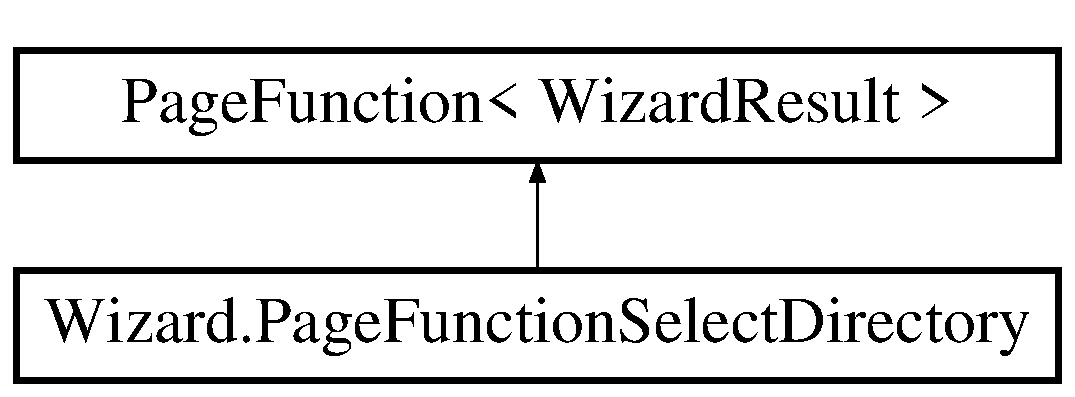
\includegraphics[height=2.000000cm]{class_wizard_1_1_page_function_select_directory}
\end{center}
\end{figure}
\subsection*{Public Member Functions}
\begin{DoxyCompactItemize}
\item 
\mbox{\Hypertarget{class_wizard_1_1_page_function_select_directory_aa0ff7c84ecd72f8b8804737cb10f6921}\label{class_wizard_1_1_page_function_select_directory_aa0ff7c84ecd72f8b8804737cb10f6921}} 
{\bfseries Page\+Function\+Select\+Directory} (\mbox{\hyperlink{class_wizard_1_1_wizard_data}{Wizard\+Data}} wizard\+Data)
\item 
\mbox{\Hypertarget{class_wizard_1_1_page_function_select_directory_ac620158dee28731a79fedd511aa6b33a}\label{class_wizard_1_1_page_function_select_directory_ac620158dee28731a79fedd511aa6b33a}} 
void {\bfseries wizard\+Page\+\_\+\+Return} (object sender, Return\+Event\+Args$<$ Wizard\+Result $>$ e)
\end{DoxyCompactItemize}


\subsection{Detailed Description}
Interaction logic for Page\+Function\+Select\+Directory.\+xaml 



Definition at line 23 of file Page\+Function\+Select\+Directory.\+xaml.\+cs.



The documentation for this class was generated from the following file\+:\begin{DoxyCompactItemize}
\item 
C\+:/\+Users/\+Shehan Vanderputt/\+Downloads/\+Compressed/\+P\+E\+D\+Scanner-\/master/\+P\+E\+D\+Scanner-\/master/\+P\+E\+D\+Scanner\+G\+U\+I\+W\+P\+F/\+P\+E\+D\+Scanner/\+P\+E\+D\+Scanner/Page\+Function\+Select\+Directory.\+xaml.\+cs\end{DoxyCompactItemize}

\hypertarget{class_wizard_1_1_page_function_select_target}{}\section{Wizard.\+Page\+Function\+Select\+Target Class Reference}
\label{class_wizard_1_1_page_function_select_target}\index{Wizard.\+Page\+Function\+Select\+Target@{Wizard.\+Page\+Function\+Select\+Target}}


Interaction logic for Page\+Function\+Select\+Target.\+xaml  


Inheritance diagram for Wizard.\+Page\+Function\+Select\+Target\+:\begin{figure}[H]
\begin{center}
\leavevmode
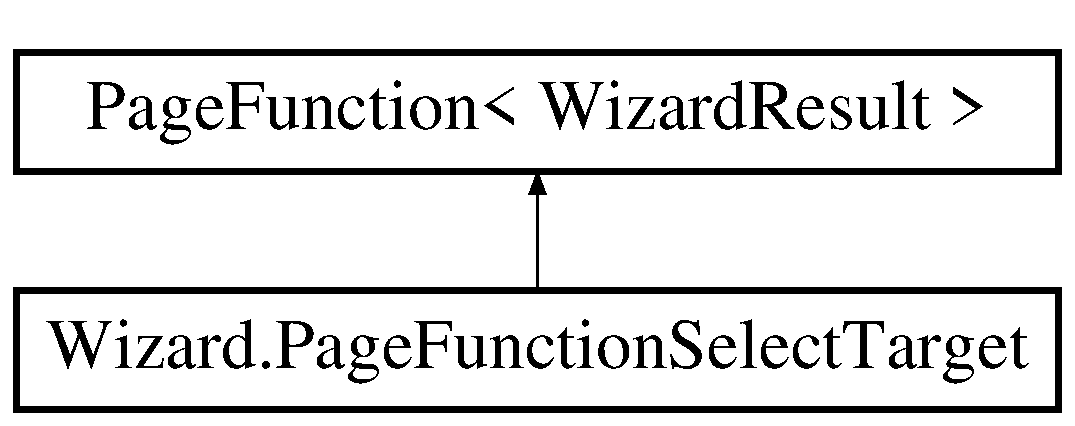
\includegraphics[height=2.000000cm]{class_wizard_1_1_page_function_select_target}
\end{center}
\end{figure}
\subsection*{Public Member Functions}
\begin{DoxyCompactItemize}
\item 
\mbox{\Hypertarget{class_wizard_1_1_page_function_select_target_a6cb77d1c6098d224a0b75f96ffdbc090}\label{class_wizard_1_1_page_function_select_target_a6cb77d1c6098d224a0b75f96ffdbc090}} 
{\bfseries Page\+Function\+Select\+Target} (\mbox{\hyperlink{class_wizard_1_1_wizard_data}{Wizard\+Data}} wizard\+Data)
\item 
\mbox{\Hypertarget{class_wizard_1_1_page_function_select_target_a7e764a36bfcebc2cf2eeafc8ee906c10}\label{class_wizard_1_1_page_function_select_target_a7e764a36bfcebc2cf2eeafc8ee906c10}} 
void {\bfseries wizard\+Page\+\_\+\+Return} (object sender, Return\+Event\+Args$<$ Wizard\+Result $>$ e)
\end{DoxyCompactItemize}


\subsection{Detailed Description}
Interaction logic for Page\+Function\+Select\+Target.\+xaml 



Definition at line 23 of file Page\+Function\+Select\+Target.\+xaml.\+cs.



The documentation for this class was generated from the following file\+:\begin{DoxyCompactItemize}
\item 
C\+:/\+Users/\+Shehan Vanderputt/\+Downloads/\+Compressed/\+P\+E\+D\+Scanner-\/master/\+P\+E\+D\+Scanner-\/master/\+P\+E\+D\+Scanner\+G\+U\+I\+W\+P\+F/\+P\+E\+D\+Scanner/\+P\+E\+D\+Scanner/Page\+Function\+Select\+Target.\+xaml.\+cs\end{DoxyCompactItemize}

\hypertarget{class_p_e_d_scanner_lib_1_1_struct_1_1_pe_header_reader}{}\section{P\+E\+D\+Scanner\+Lib.\+Struct.\+Pe\+Header\+Reader Class Reference}
\label{class_p_e_d_scanner_lib_1_1_struct_1_1_pe_header_reader}\index{P\+E\+D\+Scanner\+Lib.\+Struct.\+Pe\+Header\+Reader@{P\+E\+D\+Scanner\+Lib.\+Struct.\+Pe\+Header\+Reader}}
\subsection*{Classes}
\begin{DoxyCompactItemize}
\item 
struct \mbox{\hyperlink{struct_p_e_d_scanner_lib_1_1_struct_1_1_pe_header_reader_1_1_i_m_a_g_e___d_a_t_a___d_i_r_e_c_t_o_r_y}{I\+M\+A\+G\+E\+\_\+\+D\+A\+T\+A\+\_\+\+D\+I\+R\+E\+C\+T\+O\+RY}}
\item 
struct \mbox{\hyperlink{struct_p_e_d_scanner_lib_1_1_struct_1_1_pe_header_reader_1_1_i_m_a_g_e___d_o_s___h_e_a_d_e_r}{I\+M\+A\+G\+E\+\_\+\+D\+O\+S\+\_\+\+H\+E\+A\+D\+ER}}
\item 
struct \mbox{\hyperlink{struct_p_e_d_scanner_lib_1_1_struct_1_1_pe_header_reader_1_1_i_m_a_g_e___i_m_p_o_r_t___b_y___n_a_m_e}{I\+M\+A\+G\+E\+\_\+\+I\+M\+P\+O\+R\+T\+\_\+\+B\+Y\+\_\+\+N\+A\+ME}}
\item 
struct \mbox{\hyperlink{struct_p_e_d_scanner_lib_1_1_struct_1_1_pe_header_reader_1_1_i_m_a_g_e___i_m_p_o_r_t___d_e_s_c_r_i_p_t_o_r}{I\+M\+A\+G\+E\+\_\+\+I\+M\+P\+O\+R\+T\+\_\+\+D\+E\+S\+C\+R\+I\+P\+T\+OR}}
\item 
struct \mbox{\hyperlink{struct_p_e_d_scanner_lib_1_1_struct_1_1_pe_header_reader_1_1_i_m_a_g_e___o_p_t_i_o_n_a_l___h_e_a_d_e_r32}{I\+M\+A\+G\+E\+\_\+\+O\+P\+T\+I\+O\+N\+A\+L\+\_\+\+H\+E\+A\+D\+E\+R32}}
\item 
struct \mbox{\hyperlink{struct_p_e_d_scanner_lib_1_1_struct_1_1_pe_header_reader_1_1_i_m_a_g_e___o_p_t_i_o_n_a_l___h_e_a_d_e_r64}{I\+M\+A\+G\+E\+\_\+\+O\+P\+T\+I\+O\+N\+A\+L\+\_\+\+H\+E\+A\+D\+E\+R64}}
\item 
struct \mbox{\hyperlink{struct_p_e_d_scanner_lib_1_1_struct_1_1_pe_header_reader_1_1_i_m_a_g_e___s_e_c_t_i_o_n___h_e_a_d_e_r}{I\+M\+A\+G\+E\+\_\+\+S\+E\+C\+T\+I\+O\+N\+\_\+\+H\+E\+A\+D\+ER}}
\item 
struct \mbox{\hyperlink{struct_p_e_d_scanner_lib_1_1_struct_1_1_pe_header_reader_1_1_t_h_u_n_k___d_a_t_a}{T\+H\+U\+N\+K\+\_\+\+D\+A\+TA}}
\end{DoxyCompactItemize}
\subsection*{Public Types}
\begin{DoxyCompactItemize}
\item 
enum \mbox{\hyperlink{class_p_e_d_scanner_lib_1_1_struct_1_1_pe_header_reader_aaa653fc9f63948e6fcdc31bc79e5aeff}{Data\+Section\+Flags}} \+: uint \{ \newline
\mbox{\hyperlink{class_p_e_d_scanner_lib_1_1_struct_1_1_pe_header_reader_aaa653fc9f63948e6fcdc31bc79e5aeffac21c143fdccf061bf55b9eda845d3caf}{Data\+Section\+Flags.\+Type\+Reg}} = 0x00000000, 
\mbox{\hyperlink{class_p_e_d_scanner_lib_1_1_struct_1_1_pe_header_reader_aaa653fc9f63948e6fcdc31bc79e5aeffaa264967da0f508d66db493c2de5ee9c4}{Data\+Section\+Flags.\+Type\+Dsect}} = 0x00000001, 
\mbox{\hyperlink{class_p_e_d_scanner_lib_1_1_struct_1_1_pe_header_reader_aaa653fc9f63948e6fcdc31bc79e5aeffa7ee17105022d75d836d51057a693f05e}{Data\+Section\+Flags.\+Type\+No\+Load}} = 0x00000002, 
\mbox{\hyperlink{class_p_e_d_scanner_lib_1_1_struct_1_1_pe_header_reader_aaa653fc9f63948e6fcdc31bc79e5aeffa89fc4e991a3def4b344dc91f609ce5cd}{Data\+Section\+Flags.\+Type\+Group}} = 0x00000004, 
\newline
\mbox{\hyperlink{class_p_e_d_scanner_lib_1_1_struct_1_1_pe_header_reader_aaa653fc9f63948e6fcdc31bc79e5aeffa8afd24ddd86bd6a2da9576c97477fa6b}{Data\+Section\+Flags.\+Type\+No\+Padded}} = 0x00000008, 
\mbox{\hyperlink{class_p_e_d_scanner_lib_1_1_struct_1_1_pe_header_reader_aaa653fc9f63948e6fcdc31bc79e5aeffa91019ad316b75f1966fee3ccc7eaf8fa}{Data\+Section\+Flags.\+Type\+Copy}} = 0x00000010, 
\mbox{\hyperlink{class_p_e_d_scanner_lib_1_1_struct_1_1_pe_header_reader_aaa653fc9f63948e6fcdc31bc79e5aeffa4ec72489fe7d116e4c4c79c9da24d7a3}{Data\+Section\+Flags.\+Content\+Code}} = 0x00000020, 
\mbox{\hyperlink{class_p_e_d_scanner_lib_1_1_struct_1_1_pe_header_reader_aaa653fc9f63948e6fcdc31bc79e5aeffa8f91b9883e7678b56e62d632aae87e1d}{Data\+Section\+Flags.\+Content\+Initialized\+Data}} = 0x00000040, 
\newline
\mbox{\hyperlink{class_p_e_d_scanner_lib_1_1_struct_1_1_pe_header_reader_aaa653fc9f63948e6fcdc31bc79e5aeffaf5064527d3db43066be4ad7690bb14e6}{Data\+Section\+Flags.\+Content\+Uninitialized\+Data}} = 0x00000080, 
\mbox{\hyperlink{class_p_e_d_scanner_lib_1_1_struct_1_1_pe_header_reader_aaa653fc9f63948e6fcdc31bc79e5aeffa310ef0552dbc1a59c92660eb3f47adc1}{Data\+Section\+Flags.\+Link\+Other}} = 0x00000100, 
\mbox{\hyperlink{class_p_e_d_scanner_lib_1_1_struct_1_1_pe_header_reader_aaa653fc9f63948e6fcdc31bc79e5aeffaa428d9f343a03e0533c6eec7951dda30}{Data\+Section\+Flags.\+Link\+Info}} = 0x00000200, 
\mbox{\hyperlink{class_p_e_d_scanner_lib_1_1_struct_1_1_pe_header_reader_aaa653fc9f63948e6fcdc31bc79e5aeffa7989b8af124d838a7d198554ea1e05c7}{Data\+Section\+Flags.\+Type\+Over}} = 0x00000400, 
\newline
\mbox{\hyperlink{class_p_e_d_scanner_lib_1_1_struct_1_1_pe_header_reader_aaa653fc9f63948e6fcdc31bc79e5aeffa5924ea31a27bd099153ccc0d4e9a2bbe}{Data\+Section\+Flags.\+Link\+Remove}} = 0x00000800, 
\mbox{\hyperlink{class_p_e_d_scanner_lib_1_1_struct_1_1_pe_header_reader_aaa653fc9f63948e6fcdc31bc79e5aeffa73e94ffb5599c8e888fbbc1c4b4ff747}{Data\+Section\+Flags.\+Link\+Com\+Dat}} = 0x00001000, 
\mbox{\hyperlink{class_p_e_d_scanner_lib_1_1_struct_1_1_pe_header_reader_aaa653fc9f63948e6fcdc31bc79e5aeffa0a2c36bdae6cffdb85a207348a901c20}{Data\+Section\+Flags.\+No\+Defer\+Spec\+Exceptions}} = 0x00004000, 
\mbox{\hyperlink{class_p_e_d_scanner_lib_1_1_struct_1_1_pe_header_reader_aaa653fc9f63948e6fcdc31bc79e5aeffafbe69d00996540446cfa80fc995c4ae4}{Data\+Section\+Flags.\+Relative\+GP}} = 0x00008000, 
\newline
\mbox{\hyperlink{class_p_e_d_scanner_lib_1_1_struct_1_1_pe_header_reader_aaa653fc9f63948e6fcdc31bc79e5aeffaaf790dea4972396098fb5cac7e9e5ed9}{Data\+Section\+Flags.\+Mem\+Purgeable}} = 0x00020000, 
\mbox{\hyperlink{class_p_e_d_scanner_lib_1_1_struct_1_1_pe_header_reader_aaa653fc9f63948e6fcdc31bc79e5aeffaaf55a8c449725d41cdb4be0c1e9d509a}{Data\+Section\+Flags.\+Memory16\+Bit}} = 0x00020000, 
\mbox{\hyperlink{class_p_e_d_scanner_lib_1_1_struct_1_1_pe_header_reader_aaa653fc9f63948e6fcdc31bc79e5aeffa0e61e2d979d3a15b1c6363ad6db0d3c2}{Data\+Section\+Flags.\+Memory\+Locked}} = 0x00040000, 
\mbox{\hyperlink{class_p_e_d_scanner_lib_1_1_struct_1_1_pe_header_reader_aaa653fc9f63948e6fcdc31bc79e5aeffac681b65c0dad8c45e13ba18618bba51d}{Data\+Section\+Flags.\+Memory\+Preload}} = 0x00080000, 
\newline
\mbox{\hyperlink{class_p_e_d_scanner_lib_1_1_struct_1_1_pe_header_reader_aaa653fc9f63948e6fcdc31bc79e5aeffa765608de9ac729fa6119f33d86323641}{Data\+Section\+Flags.\+Align1\+Bytes}} = 0x00100000, 
\mbox{\hyperlink{class_p_e_d_scanner_lib_1_1_struct_1_1_pe_header_reader_aaa653fc9f63948e6fcdc31bc79e5aeffabda3bf76a97acf1e08d8d8dc88fdb67a}{Data\+Section\+Flags.\+Align2\+Bytes}} = 0x00200000, 
\mbox{\hyperlink{class_p_e_d_scanner_lib_1_1_struct_1_1_pe_header_reader_aaa653fc9f63948e6fcdc31bc79e5aeffa05f653feb004753aa92651687c087bf4}{Data\+Section\+Flags.\+Align4\+Bytes}} = 0x00300000, 
\mbox{\hyperlink{class_p_e_d_scanner_lib_1_1_struct_1_1_pe_header_reader_aaa653fc9f63948e6fcdc31bc79e5aeffa9c81f9390bd6e5fdc3c644d7684e54cd}{Data\+Section\+Flags.\+Align8\+Bytes}} = 0x00400000, 
\newline
\mbox{\hyperlink{class_p_e_d_scanner_lib_1_1_struct_1_1_pe_header_reader_aaa653fc9f63948e6fcdc31bc79e5aeffa1624fde44c1dc0e9d9570d83e88b1b3b}{Data\+Section\+Flags.\+Align16\+Bytes}} = 0x00500000, 
\mbox{\hyperlink{class_p_e_d_scanner_lib_1_1_struct_1_1_pe_header_reader_aaa653fc9f63948e6fcdc31bc79e5aeffa4a584494f73a30648222bb89e35830be}{Data\+Section\+Flags.\+Align32\+Bytes}} = 0x00600000, 
\mbox{\hyperlink{class_p_e_d_scanner_lib_1_1_struct_1_1_pe_header_reader_aaa653fc9f63948e6fcdc31bc79e5aeffaefeec26f9afb6e00df49a0acffd16e90}{Data\+Section\+Flags.\+Align64\+Bytes}} = 0x00700000, 
\mbox{\hyperlink{class_p_e_d_scanner_lib_1_1_struct_1_1_pe_header_reader_aaa653fc9f63948e6fcdc31bc79e5aeffa317428f01d0052902a8e55741bd564c9}{Data\+Section\+Flags.\+Align128\+Bytes}} = 0x00800000, 
\newline
\mbox{\hyperlink{class_p_e_d_scanner_lib_1_1_struct_1_1_pe_header_reader_aaa653fc9f63948e6fcdc31bc79e5aeffad4d21d5a24fb77f60d2ad18560454857}{Data\+Section\+Flags.\+Align256\+Bytes}} = 0x00900000, 
\mbox{\hyperlink{class_p_e_d_scanner_lib_1_1_struct_1_1_pe_header_reader_aaa653fc9f63948e6fcdc31bc79e5aeffa2cb33ad220460fc67eb9df43ac9cc988}{Data\+Section\+Flags.\+Align512\+Bytes}} = 0x00\+A00000, 
\mbox{\hyperlink{class_p_e_d_scanner_lib_1_1_struct_1_1_pe_header_reader_aaa653fc9f63948e6fcdc31bc79e5aeffa9f224b78990bba5f417cacf3cf44a236}{Data\+Section\+Flags.\+Align1024\+Bytes}} = 0x00\+B00000, 
\mbox{\hyperlink{class_p_e_d_scanner_lib_1_1_struct_1_1_pe_header_reader_aaa653fc9f63948e6fcdc31bc79e5aeffa7b58be045531f536c602fbf4b6a5cc3e}{Data\+Section\+Flags.\+Align2048\+Bytes}} = 0x00\+C00000, 
\newline
\mbox{\hyperlink{class_p_e_d_scanner_lib_1_1_struct_1_1_pe_header_reader_aaa653fc9f63948e6fcdc31bc79e5aeffa9243d8888148599e989aec20216879e6}{Data\+Section\+Flags.\+Align4096\+Bytes}} = 0x00\+D00000, 
\mbox{\hyperlink{class_p_e_d_scanner_lib_1_1_struct_1_1_pe_header_reader_aaa653fc9f63948e6fcdc31bc79e5aeffa9306df9231ab5bd52e25a8b279a2ec55}{Data\+Section\+Flags.\+Align8192\+Bytes}} = 0x00\+E00000, 
\mbox{\hyperlink{class_p_e_d_scanner_lib_1_1_struct_1_1_pe_header_reader_aaa653fc9f63948e6fcdc31bc79e5aeffad01894da5465bddb53ddde319dfe19b3}{Data\+Section\+Flags.\+Link\+Extended\+Relocation\+Overflow}} = 0x01000000, 
\mbox{\hyperlink{class_p_e_d_scanner_lib_1_1_struct_1_1_pe_header_reader_aaa653fc9f63948e6fcdc31bc79e5aeffa5709064f25349c396c44922d4fab6fbe}{Data\+Section\+Flags.\+Memory\+Discardable}} = 0x02000000, 
\newline
\mbox{\hyperlink{class_p_e_d_scanner_lib_1_1_struct_1_1_pe_header_reader_aaa653fc9f63948e6fcdc31bc79e5aeffa464fabb621c581183a5c410fc2ca7c7f}{Data\+Section\+Flags.\+Memory\+Not\+Cached}} = 0x04000000, 
\mbox{\hyperlink{class_p_e_d_scanner_lib_1_1_struct_1_1_pe_header_reader_aaa653fc9f63948e6fcdc31bc79e5aeffaf17f8f106acef3fd0ff47b8cca4de356}{Data\+Section\+Flags.\+Memory\+Not\+Paged}} = 0x08000000, 
\mbox{\hyperlink{class_p_e_d_scanner_lib_1_1_struct_1_1_pe_header_reader_aaa653fc9f63948e6fcdc31bc79e5aeffabfa33c37b72f766266c354cb6eb01d3a}{Data\+Section\+Flags.\+Memory\+Shared}} = 0x10000000, 
\mbox{\hyperlink{class_p_e_d_scanner_lib_1_1_struct_1_1_pe_header_reader_aaa653fc9f63948e6fcdc31bc79e5aeffa817041d31daef398c32f9e2efc8c482f}{Data\+Section\+Flags.\+Memory\+Execute}} = 0x20000000, 
\newline
\mbox{\hyperlink{class_p_e_d_scanner_lib_1_1_struct_1_1_pe_header_reader_aaa653fc9f63948e6fcdc31bc79e5aeffa575da5d1d4109b111267b2e044af2aad}{Data\+Section\+Flags.\+Memory\+Read}} = 0x40000000, 
\mbox{\hyperlink{class_p_e_d_scanner_lib_1_1_struct_1_1_pe_header_reader_aaa653fc9f63948e6fcdc31bc79e5aeffa5e932342aab40efaef1a503864403168}{Data\+Section\+Flags.\+Memory\+Write}} = 0x80000000
 \}
\end{DoxyCompactItemize}
\subsection*{Public Member Functions}
\begin{DoxyCompactItemize}
\item 
\mbox{\Hypertarget{class_p_e_d_scanner_lib_1_1_struct_1_1_pe_header_reader_a97d98fa574c08071ed498586314d4caa}\label{class_p_e_d_scanner_lib_1_1_struct_1_1_pe_header_reader_a97d98fa574c08071ed498586314d4caa}} 
{\bfseries Pe\+Header\+Reader} (string file\+Path)
\end{DoxyCompactItemize}
\subsection*{Static Public Member Functions}
\begin{DoxyCompactItemize}
\item 
\mbox{\Hypertarget{class_p_e_d_scanner_lib_1_1_struct_1_1_pe_header_reader_adf4919d95e52a3ce89567a69f2081281}\label{class_p_e_d_scanner_lib_1_1_struct_1_1_pe_header_reader_adf4919d95e52a3ce89567a69f2081281}} 
static T {\bfseries From\+Binary\+Reader$<$ T $>$} (Binary\+Reader reader)
\end{DoxyCompactItemize}
\subsection*{Properties}
\begin{DoxyCompactItemize}
\item 
bool \mbox{\hyperlink{class_p_e_d_scanner_lib_1_1_struct_1_1_pe_header_reader_ab7c430566cf03dd2f912b227cc3ce429}{Is32\+Bit\+Header}}\hspace{0.3cm}{\ttfamily  \mbox{[}get\mbox{]}}
\begin{DoxyCompactList}\small\item\em Gets if the file header is 32 bit or not \end{DoxyCompactList}\item 
\mbox{\hyperlink{struct_p_e_d_scanner_lib_1_1_struct_1_1_i_m_a_g_e___f_i_l_e___h_e_a_d_e_r}{I\+M\+A\+G\+E\+\_\+\+F\+I\+L\+E\+\_\+\+H\+E\+A\+D\+ER}} \mbox{\hyperlink{class_p_e_d_scanner_lib_1_1_struct_1_1_pe_header_reader_a58745ae2d2707ed46590335ac7c8b6b2}{File\+Header}}\hspace{0.3cm}{\ttfamily  \mbox{[}get\mbox{]}}
\begin{DoxyCompactList}\small\item\em Gets the file header \end{DoxyCompactList}\item 
\mbox{\hyperlink{struct_p_e_d_scanner_lib_1_1_struct_1_1_pe_header_reader_1_1_i_m_a_g_e___o_p_t_i_o_n_a_l___h_e_a_d_e_r32}{I\+M\+A\+G\+E\+\_\+\+O\+P\+T\+I\+O\+N\+A\+L\+\_\+\+H\+E\+A\+D\+E\+R32}} \mbox{\hyperlink{class_p_e_d_scanner_lib_1_1_struct_1_1_pe_header_reader_ae4fcbb233eaeb2cc2835d5a910e5bf92}{Optional\+Header32}}\hspace{0.3cm}{\ttfamily  \mbox{[}get\mbox{]}}
\begin{DoxyCompactList}\small\item\em Gets the optional header \end{DoxyCompactList}\item 
\mbox{\hyperlink{struct_p_e_d_scanner_lib_1_1_struct_1_1_pe_header_reader_1_1_i_m_a_g_e___o_p_t_i_o_n_a_l___h_e_a_d_e_r64}{I\+M\+A\+G\+E\+\_\+\+O\+P\+T\+I\+O\+N\+A\+L\+\_\+\+H\+E\+A\+D\+E\+R64}} \mbox{\hyperlink{class_p_e_d_scanner_lib_1_1_struct_1_1_pe_header_reader_a59db8bf8f6afa28f5fa3f337b13fa1a0}{Optional\+Header64}}\hspace{0.3cm}{\ttfamily  \mbox{[}get\mbox{]}}
\begin{DoxyCompactList}\small\item\em Gets the optional header \end{DoxyCompactList}\item 
\mbox{\Hypertarget{class_p_e_d_scanner_lib_1_1_struct_1_1_pe_header_reader_a7ada7b0eed1c6181c2e2a7288c22c146}\label{class_p_e_d_scanner_lib_1_1_struct_1_1_pe_header_reader_a7ada7b0eed1c6181c2e2a7288c22c146}} 
\mbox{\hyperlink{struct_p_e_d_scanner_lib_1_1_struct_1_1_pe_header_reader_1_1_i_m_a_g_e___s_e_c_t_i_o_n___h_e_a_d_e_r}{I\+M\+A\+G\+E\+\_\+\+S\+E\+C\+T\+I\+O\+N\+\_\+\+H\+E\+A\+D\+ER}} \mbox{[}$\,$\mbox{]} {\bfseries Image\+Section\+Headers}\hspace{0.3cm}{\ttfamily  \mbox{[}get\mbox{]}}
\end{DoxyCompactItemize}


\subsection{Detailed Description}


Definition at line 356 of file Native\+Dll\+Structs.\+cs.



\subsection{Member Enumeration Documentation}
\mbox{\Hypertarget{class_p_e_d_scanner_lib_1_1_struct_1_1_pe_header_reader_aaa653fc9f63948e6fcdc31bc79e5aeff}\label{class_p_e_d_scanner_lib_1_1_struct_1_1_pe_header_reader_aaa653fc9f63948e6fcdc31bc79e5aeff}} 
\index{P\+E\+D\+Scanner\+Lib\+::\+Struct\+::\+Pe\+Header\+Reader@{P\+E\+D\+Scanner\+Lib\+::\+Struct\+::\+Pe\+Header\+Reader}!Data\+Section\+Flags@{Data\+Section\+Flags}}
\index{Data\+Section\+Flags@{Data\+Section\+Flags}!P\+E\+D\+Scanner\+Lib\+::\+Struct\+::\+Pe\+Header\+Reader@{P\+E\+D\+Scanner\+Lib\+::\+Struct\+::\+Pe\+Header\+Reader}}
\subsubsection{\texorpdfstring{Data\+Section\+Flags}{DataSectionFlags}}
{\footnotesize\ttfamily enum \mbox{\hyperlink{class_p_e_d_scanner_lib_1_1_struct_1_1_pe_header_reader_aaa653fc9f63948e6fcdc31bc79e5aeff}{P\+E\+D\+Scanner\+Lib.\+Struct.\+Pe\+Header\+Reader.\+Data\+Section\+Flags}} \+: uint\hspace{0.3cm}{\ttfamily [strong]}}

\begin{DoxyEnumFields}{Enumerator}
\raisebox{\heightof{T}}[0pt][0pt]{\index{Type\+Reg@{Type\+Reg}!P\+E\+D\+Scanner\+Lib\+::\+Struct\+::\+Pe\+Header\+Reader@{P\+E\+D\+Scanner\+Lib\+::\+Struct\+::\+Pe\+Header\+Reader}}\index{P\+E\+D\+Scanner\+Lib\+::\+Struct\+::\+Pe\+Header\+Reader@{P\+E\+D\+Scanner\+Lib\+::\+Struct\+::\+Pe\+Header\+Reader}!Type\+Reg@{Type\+Reg}}}\mbox{\Hypertarget{class_p_e_d_scanner_lib_1_1_struct_1_1_pe_header_reader_aaa653fc9f63948e6fcdc31bc79e5aeffac21c143fdccf061bf55b9eda845d3caf}\label{class_p_e_d_scanner_lib_1_1_struct_1_1_pe_header_reader_aaa653fc9f63948e6fcdc31bc79e5aeffac21c143fdccf061bf55b9eda845d3caf}} 
Type\+Reg&Reserved for future use. \\
\hline

\raisebox{\heightof{T}}[0pt][0pt]{\index{Type\+Dsect@{Type\+Dsect}!P\+E\+D\+Scanner\+Lib\+::\+Struct\+::\+Pe\+Header\+Reader@{P\+E\+D\+Scanner\+Lib\+::\+Struct\+::\+Pe\+Header\+Reader}}\index{P\+E\+D\+Scanner\+Lib\+::\+Struct\+::\+Pe\+Header\+Reader@{P\+E\+D\+Scanner\+Lib\+::\+Struct\+::\+Pe\+Header\+Reader}!Type\+Dsect@{Type\+Dsect}}}\mbox{\Hypertarget{class_p_e_d_scanner_lib_1_1_struct_1_1_pe_header_reader_aaa653fc9f63948e6fcdc31bc79e5aeffaa264967da0f508d66db493c2de5ee9c4}\label{class_p_e_d_scanner_lib_1_1_struct_1_1_pe_header_reader_aaa653fc9f63948e6fcdc31bc79e5aeffaa264967da0f508d66db493c2de5ee9c4}} 
Type\+Dsect&Reserved for future use. \\
\hline

\raisebox{\heightof{T}}[0pt][0pt]{\index{Type\+No\+Load@{Type\+No\+Load}!P\+E\+D\+Scanner\+Lib\+::\+Struct\+::\+Pe\+Header\+Reader@{P\+E\+D\+Scanner\+Lib\+::\+Struct\+::\+Pe\+Header\+Reader}}\index{P\+E\+D\+Scanner\+Lib\+::\+Struct\+::\+Pe\+Header\+Reader@{P\+E\+D\+Scanner\+Lib\+::\+Struct\+::\+Pe\+Header\+Reader}!Type\+No\+Load@{Type\+No\+Load}}}\mbox{\Hypertarget{class_p_e_d_scanner_lib_1_1_struct_1_1_pe_header_reader_aaa653fc9f63948e6fcdc31bc79e5aeffa7ee17105022d75d836d51057a693f05e}\label{class_p_e_d_scanner_lib_1_1_struct_1_1_pe_header_reader_aaa653fc9f63948e6fcdc31bc79e5aeffa7ee17105022d75d836d51057a693f05e}} 
Type\+No\+Load&Reserved for future use. \\
\hline

\raisebox{\heightof{T}}[0pt][0pt]{\index{Type\+Group@{Type\+Group}!P\+E\+D\+Scanner\+Lib\+::\+Struct\+::\+Pe\+Header\+Reader@{P\+E\+D\+Scanner\+Lib\+::\+Struct\+::\+Pe\+Header\+Reader}}\index{P\+E\+D\+Scanner\+Lib\+::\+Struct\+::\+Pe\+Header\+Reader@{P\+E\+D\+Scanner\+Lib\+::\+Struct\+::\+Pe\+Header\+Reader}!Type\+Group@{Type\+Group}}}\mbox{\Hypertarget{class_p_e_d_scanner_lib_1_1_struct_1_1_pe_header_reader_aaa653fc9f63948e6fcdc31bc79e5aeffa89fc4e991a3def4b344dc91f609ce5cd}\label{class_p_e_d_scanner_lib_1_1_struct_1_1_pe_header_reader_aaa653fc9f63948e6fcdc31bc79e5aeffa89fc4e991a3def4b344dc91f609ce5cd}} 
Type\+Group&Reserved for future use. \\
\hline

\raisebox{\heightof{T}}[0pt][0pt]{\index{Type\+No\+Padded@{Type\+No\+Padded}!P\+E\+D\+Scanner\+Lib\+::\+Struct\+::\+Pe\+Header\+Reader@{P\+E\+D\+Scanner\+Lib\+::\+Struct\+::\+Pe\+Header\+Reader}}\index{P\+E\+D\+Scanner\+Lib\+::\+Struct\+::\+Pe\+Header\+Reader@{P\+E\+D\+Scanner\+Lib\+::\+Struct\+::\+Pe\+Header\+Reader}!Type\+No\+Padded@{Type\+No\+Padded}}}\mbox{\Hypertarget{class_p_e_d_scanner_lib_1_1_struct_1_1_pe_header_reader_aaa653fc9f63948e6fcdc31bc79e5aeffa8afd24ddd86bd6a2da9576c97477fa6b}\label{class_p_e_d_scanner_lib_1_1_struct_1_1_pe_header_reader_aaa653fc9f63948e6fcdc31bc79e5aeffa8afd24ddd86bd6a2da9576c97477fa6b}} 
Type\+No\+Padded&The section should not be padded to the next boundary. This flag is obsolete and is replaced by I\+M\+A\+G\+E\+\_\+\+S\+C\+N\+\_\+\+A\+L\+I\+G\+N\+\_\+1\+B\+Y\+T\+ES. This is valid only for object files. \\
\hline

\raisebox{\heightof{T}}[0pt][0pt]{\index{Type\+Copy@{Type\+Copy}!P\+E\+D\+Scanner\+Lib\+::\+Struct\+::\+Pe\+Header\+Reader@{P\+E\+D\+Scanner\+Lib\+::\+Struct\+::\+Pe\+Header\+Reader}}\index{P\+E\+D\+Scanner\+Lib\+::\+Struct\+::\+Pe\+Header\+Reader@{P\+E\+D\+Scanner\+Lib\+::\+Struct\+::\+Pe\+Header\+Reader}!Type\+Copy@{Type\+Copy}}}\mbox{\Hypertarget{class_p_e_d_scanner_lib_1_1_struct_1_1_pe_header_reader_aaa653fc9f63948e6fcdc31bc79e5aeffa91019ad316b75f1966fee3ccc7eaf8fa}\label{class_p_e_d_scanner_lib_1_1_struct_1_1_pe_header_reader_aaa653fc9f63948e6fcdc31bc79e5aeffa91019ad316b75f1966fee3ccc7eaf8fa}} 
Type\+Copy&Reserved for future use. \\
\hline

\raisebox{\heightof{T}}[0pt][0pt]{\index{Content\+Code@{Content\+Code}!P\+E\+D\+Scanner\+Lib\+::\+Struct\+::\+Pe\+Header\+Reader@{P\+E\+D\+Scanner\+Lib\+::\+Struct\+::\+Pe\+Header\+Reader}}\index{P\+E\+D\+Scanner\+Lib\+::\+Struct\+::\+Pe\+Header\+Reader@{P\+E\+D\+Scanner\+Lib\+::\+Struct\+::\+Pe\+Header\+Reader}!Content\+Code@{Content\+Code}}}\mbox{\Hypertarget{class_p_e_d_scanner_lib_1_1_struct_1_1_pe_header_reader_aaa653fc9f63948e6fcdc31bc79e5aeffa4ec72489fe7d116e4c4c79c9da24d7a3}\label{class_p_e_d_scanner_lib_1_1_struct_1_1_pe_header_reader_aaa653fc9f63948e6fcdc31bc79e5aeffa4ec72489fe7d116e4c4c79c9da24d7a3}} 
Content\+Code&The section contains executable code. \\
\hline

\raisebox{\heightof{T}}[0pt][0pt]{\index{Content\+Initialized\+Data@{Content\+Initialized\+Data}!P\+E\+D\+Scanner\+Lib\+::\+Struct\+::\+Pe\+Header\+Reader@{P\+E\+D\+Scanner\+Lib\+::\+Struct\+::\+Pe\+Header\+Reader}}\index{P\+E\+D\+Scanner\+Lib\+::\+Struct\+::\+Pe\+Header\+Reader@{P\+E\+D\+Scanner\+Lib\+::\+Struct\+::\+Pe\+Header\+Reader}!Content\+Initialized\+Data@{Content\+Initialized\+Data}}}\mbox{\Hypertarget{class_p_e_d_scanner_lib_1_1_struct_1_1_pe_header_reader_aaa653fc9f63948e6fcdc31bc79e5aeffa8f91b9883e7678b56e62d632aae87e1d}\label{class_p_e_d_scanner_lib_1_1_struct_1_1_pe_header_reader_aaa653fc9f63948e6fcdc31bc79e5aeffa8f91b9883e7678b56e62d632aae87e1d}} 
Content\+Initialized\+Data&The section contains initialized data. \\
\hline

\raisebox{\heightof{T}}[0pt][0pt]{\index{Content\+Uninitialized\+Data@{Content\+Uninitialized\+Data}!P\+E\+D\+Scanner\+Lib\+::\+Struct\+::\+Pe\+Header\+Reader@{P\+E\+D\+Scanner\+Lib\+::\+Struct\+::\+Pe\+Header\+Reader}}\index{P\+E\+D\+Scanner\+Lib\+::\+Struct\+::\+Pe\+Header\+Reader@{P\+E\+D\+Scanner\+Lib\+::\+Struct\+::\+Pe\+Header\+Reader}!Content\+Uninitialized\+Data@{Content\+Uninitialized\+Data}}}\mbox{\Hypertarget{class_p_e_d_scanner_lib_1_1_struct_1_1_pe_header_reader_aaa653fc9f63948e6fcdc31bc79e5aeffaf5064527d3db43066be4ad7690bb14e6}\label{class_p_e_d_scanner_lib_1_1_struct_1_1_pe_header_reader_aaa653fc9f63948e6fcdc31bc79e5aeffaf5064527d3db43066be4ad7690bb14e6}} 
Content\+Uninitialized\+Data&The section contains uninitialized data. \\
\hline

\raisebox{\heightof{T}}[0pt][0pt]{\index{Link\+Other@{Link\+Other}!P\+E\+D\+Scanner\+Lib\+::\+Struct\+::\+Pe\+Header\+Reader@{P\+E\+D\+Scanner\+Lib\+::\+Struct\+::\+Pe\+Header\+Reader}}\index{P\+E\+D\+Scanner\+Lib\+::\+Struct\+::\+Pe\+Header\+Reader@{P\+E\+D\+Scanner\+Lib\+::\+Struct\+::\+Pe\+Header\+Reader}!Link\+Other@{Link\+Other}}}\mbox{\Hypertarget{class_p_e_d_scanner_lib_1_1_struct_1_1_pe_header_reader_aaa653fc9f63948e6fcdc31bc79e5aeffa310ef0552dbc1a59c92660eb3f47adc1}\label{class_p_e_d_scanner_lib_1_1_struct_1_1_pe_header_reader_aaa653fc9f63948e6fcdc31bc79e5aeffa310ef0552dbc1a59c92660eb3f47adc1}} 
Link\+Other&Reserved for future use. \\
\hline

\raisebox{\heightof{T}}[0pt][0pt]{\index{Link\+Info@{Link\+Info}!P\+E\+D\+Scanner\+Lib\+::\+Struct\+::\+Pe\+Header\+Reader@{P\+E\+D\+Scanner\+Lib\+::\+Struct\+::\+Pe\+Header\+Reader}}\index{P\+E\+D\+Scanner\+Lib\+::\+Struct\+::\+Pe\+Header\+Reader@{P\+E\+D\+Scanner\+Lib\+::\+Struct\+::\+Pe\+Header\+Reader}!Link\+Info@{Link\+Info}}}\mbox{\Hypertarget{class_p_e_d_scanner_lib_1_1_struct_1_1_pe_header_reader_aaa653fc9f63948e6fcdc31bc79e5aeffaa428d9f343a03e0533c6eec7951dda30}\label{class_p_e_d_scanner_lib_1_1_struct_1_1_pe_header_reader_aaa653fc9f63948e6fcdc31bc79e5aeffaa428d9f343a03e0533c6eec7951dda30}} 
Link\+Info&The section contains comments or other information. The .drectve section has this type. This is valid for object files only. \\
\hline

\raisebox{\heightof{T}}[0pt][0pt]{\index{Type\+Over@{Type\+Over}!P\+E\+D\+Scanner\+Lib\+::\+Struct\+::\+Pe\+Header\+Reader@{P\+E\+D\+Scanner\+Lib\+::\+Struct\+::\+Pe\+Header\+Reader}}\index{P\+E\+D\+Scanner\+Lib\+::\+Struct\+::\+Pe\+Header\+Reader@{P\+E\+D\+Scanner\+Lib\+::\+Struct\+::\+Pe\+Header\+Reader}!Type\+Over@{Type\+Over}}}\mbox{\Hypertarget{class_p_e_d_scanner_lib_1_1_struct_1_1_pe_header_reader_aaa653fc9f63948e6fcdc31bc79e5aeffa7989b8af124d838a7d198554ea1e05c7}\label{class_p_e_d_scanner_lib_1_1_struct_1_1_pe_header_reader_aaa653fc9f63948e6fcdc31bc79e5aeffa7989b8af124d838a7d198554ea1e05c7}} 
Type\+Over&Reserved for future use. \\
\hline

\raisebox{\heightof{T}}[0pt][0pt]{\index{Link\+Remove@{Link\+Remove}!P\+E\+D\+Scanner\+Lib\+::\+Struct\+::\+Pe\+Header\+Reader@{P\+E\+D\+Scanner\+Lib\+::\+Struct\+::\+Pe\+Header\+Reader}}\index{P\+E\+D\+Scanner\+Lib\+::\+Struct\+::\+Pe\+Header\+Reader@{P\+E\+D\+Scanner\+Lib\+::\+Struct\+::\+Pe\+Header\+Reader}!Link\+Remove@{Link\+Remove}}}\mbox{\Hypertarget{class_p_e_d_scanner_lib_1_1_struct_1_1_pe_header_reader_aaa653fc9f63948e6fcdc31bc79e5aeffa5924ea31a27bd099153ccc0d4e9a2bbe}\label{class_p_e_d_scanner_lib_1_1_struct_1_1_pe_header_reader_aaa653fc9f63948e6fcdc31bc79e5aeffa5924ea31a27bd099153ccc0d4e9a2bbe}} 
Link\+Remove&The section will not become part of the image. This is valid only for object files. \\
\hline

\raisebox{\heightof{T}}[0pt][0pt]{\index{Link\+Com\+Dat@{Link\+Com\+Dat}!P\+E\+D\+Scanner\+Lib\+::\+Struct\+::\+Pe\+Header\+Reader@{P\+E\+D\+Scanner\+Lib\+::\+Struct\+::\+Pe\+Header\+Reader}}\index{P\+E\+D\+Scanner\+Lib\+::\+Struct\+::\+Pe\+Header\+Reader@{P\+E\+D\+Scanner\+Lib\+::\+Struct\+::\+Pe\+Header\+Reader}!Link\+Com\+Dat@{Link\+Com\+Dat}}}\mbox{\Hypertarget{class_p_e_d_scanner_lib_1_1_struct_1_1_pe_header_reader_aaa653fc9f63948e6fcdc31bc79e5aeffa73e94ffb5599c8e888fbbc1c4b4ff747}\label{class_p_e_d_scanner_lib_1_1_struct_1_1_pe_header_reader_aaa653fc9f63948e6fcdc31bc79e5aeffa73e94ffb5599c8e888fbbc1c4b4ff747}} 
Link\+Com\+Dat&The section contains C\+O\+M\+D\+AT data. For more information, see section 5.\+5.\+6, C\+O\+M\+D\+AT Sections (Object Only). This is valid only for object files. \\
\hline

\raisebox{\heightof{T}}[0pt][0pt]{\index{No\+Defer\+Spec\+Exceptions@{No\+Defer\+Spec\+Exceptions}!P\+E\+D\+Scanner\+Lib\+::\+Struct\+::\+Pe\+Header\+Reader@{P\+E\+D\+Scanner\+Lib\+::\+Struct\+::\+Pe\+Header\+Reader}}\index{P\+E\+D\+Scanner\+Lib\+::\+Struct\+::\+Pe\+Header\+Reader@{P\+E\+D\+Scanner\+Lib\+::\+Struct\+::\+Pe\+Header\+Reader}!No\+Defer\+Spec\+Exceptions@{No\+Defer\+Spec\+Exceptions}}}\mbox{\Hypertarget{class_p_e_d_scanner_lib_1_1_struct_1_1_pe_header_reader_aaa653fc9f63948e6fcdc31bc79e5aeffa0a2c36bdae6cffdb85a207348a901c20}\label{class_p_e_d_scanner_lib_1_1_struct_1_1_pe_header_reader_aaa653fc9f63948e6fcdc31bc79e5aeffa0a2c36bdae6cffdb85a207348a901c20}} 
No\+Defer\+Spec\+Exceptions&Reset speculative exceptions handling bits in the T\+LB entries for this section. \\
\hline

\raisebox{\heightof{T}}[0pt][0pt]{\index{Relative\+GP@{Relative\+GP}!P\+E\+D\+Scanner\+Lib\+::\+Struct\+::\+Pe\+Header\+Reader@{P\+E\+D\+Scanner\+Lib\+::\+Struct\+::\+Pe\+Header\+Reader}}\index{P\+E\+D\+Scanner\+Lib\+::\+Struct\+::\+Pe\+Header\+Reader@{P\+E\+D\+Scanner\+Lib\+::\+Struct\+::\+Pe\+Header\+Reader}!Relative\+GP@{Relative\+GP}}}\mbox{\Hypertarget{class_p_e_d_scanner_lib_1_1_struct_1_1_pe_header_reader_aaa653fc9f63948e6fcdc31bc79e5aeffafbe69d00996540446cfa80fc995c4ae4}\label{class_p_e_d_scanner_lib_1_1_struct_1_1_pe_header_reader_aaa653fc9f63948e6fcdc31bc79e5aeffafbe69d00996540446cfa80fc995c4ae4}} 
Relative\+GP&The section contains data referenced through the global pointer (GP). \\
\hline

\raisebox{\heightof{T}}[0pt][0pt]{\index{Mem\+Purgeable@{Mem\+Purgeable}!P\+E\+D\+Scanner\+Lib\+::\+Struct\+::\+Pe\+Header\+Reader@{P\+E\+D\+Scanner\+Lib\+::\+Struct\+::\+Pe\+Header\+Reader}}\index{P\+E\+D\+Scanner\+Lib\+::\+Struct\+::\+Pe\+Header\+Reader@{P\+E\+D\+Scanner\+Lib\+::\+Struct\+::\+Pe\+Header\+Reader}!Mem\+Purgeable@{Mem\+Purgeable}}}\mbox{\Hypertarget{class_p_e_d_scanner_lib_1_1_struct_1_1_pe_header_reader_aaa653fc9f63948e6fcdc31bc79e5aeffaaf790dea4972396098fb5cac7e9e5ed9}\label{class_p_e_d_scanner_lib_1_1_struct_1_1_pe_header_reader_aaa653fc9f63948e6fcdc31bc79e5aeffaaf790dea4972396098fb5cac7e9e5ed9}} 
Mem\+Purgeable&Reserved for future use. \\
\hline

\raisebox{\heightof{T}}[0pt][0pt]{\index{Memory16\+Bit@{Memory16\+Bit}!P\+E\+D\+Scanner\+Lib\+::\+Struct\+::\+Pe\+Header\+Reader@{P\+E\+D\+Scanner\+Lib\+::\+Struct\+::\+Pe\+Header\+Reader}}\index{P\+E\+D\+Scanner\+Lib\+::\+Struct\+::\+Pe\+Header\+Reader@{P\+E\+D\+Scanner\+Lib\+::\+Struct\+::\+Pe\+Header\+Reader}!Memory16\+Bit@{Memory16\+Bit}}}\mbox{\Hypertarget{class_p_e_d_scanner_lib_1_1_struct_1_1_pe_header_reader_aaa653fc9f63948e6fcdc31bc79e5aeffaaf55a8c449725d41cdb4be0c1e9d509a}\label{class_p_e_d_scanner_lib_1_1_struct_1_1_pe_header_reader_aaa653fc9f63948e6fcdc31bc79e5aeffaaf55a8c449725d41cdb4be0c1e9d509a}} 
Memory16\+Bit&Reserved for future use. \\
\hline

\raisebox{\heightof{T}}[0pt][0pt]{\index{Memory\+Locked@{Memory\+Locked}!P\+E\+D\+Scanner\+Lib\+::\+Struct\+::\+Pe\+Header\+Reader@{P\+E\+D\+Scanner\+Lib\+::\+Struct\+::\+Pe\+Header\+Reader}}\index{P\+E\+D\+Scanner\+Lib\+::\+Struct\+::\+Pe\+Header\+Reader@{P\+E\+D\+Scanner\+Lib\+::\+Struct\+::\+Pe\+Header\+Reader}!Memory\+Locked@{Memory\+Locked}}}\mbox{\Hypertarget{class_p_e_d_scanner_lib_1_1_struct_1_1_pe_header_reader_aaa653fc9f63948e6fcdc31bc79e5aeffa0e61e2d979d3a15b1c6363ad6db0d3c2}\label{class_p_e_d_scanner_lib_1_1_struct_1_1_pe_header_reader_aaa653fc9f63948e6fcdc31bc79e5aeffa0e61e2d979d3a15b1c6363ad6db0d3c2}} 
Memory\+Locked&Reserved for future use. \\
\hline

\raisebox{\heightof{T}}[0pt][0pt]{\index{Memory\+Preload@{Memory\+Preload}!P\+E\+D\+Scanner\+Lib\+::\+Struct\+::\+Pe\+Header\+Reader@{P\+E\+D\+Scanner\+Lib\+::\+Struct\+::\+Pe\+Header\+Reader}}\index{P\+E\+D\+Scanner\+Lib\+::\+Struct\+::\+Pe\+Header\+Reader@{P\+E\+D\+Scanner\+Lib\+::\+Struct\+::\+Pe\+Header\+Reader}!Memory\+Preload@{Memory\+Preload}}}\mbox{\Hypertarget{class_p_e_d_scanner_lib_1_1_struct_1_1_pe_header_reader_aaa653fc9f63948e6fcdc31bc79e5aeffac681b65c0dad8c45e13ba18618bba51d}\label{class_p_e_d_scanner_lib_1_1_struct_1_1_pe_header_reader_aaa653fc9f63948e6fcdc31bc79e5aeffac681b65c0dad8c45e13ba18618bba51d}} 
Memory\+Preload&Reserved for future use. \\
\hline

\raisebox{\heightof{T}}[0pt][0pt]{\index{Align1\+Bytes@{Align1\+Bytes}!P\+E\+D\+Scanner\+Lib\+::\+Struct\+::\+Pe\+Header\+Reader@{P\+E\+D\+Scanner\+Lib\+::\+Struct\+::\+Pe\+Header\+Reader}}\index{P\+E\+D\+Scanner\+Lib\+::\+Struct\+::\+Pe\+Header\+Reader@{P\+E\+D\+Scanner\+Lib\+::\+Struct\+::\+Pe\+Header\+Reader}!Align1\+Bytes@{Align1\+Bytes}}}\mbox{\Hypertarget{class_p_e_d_scanner_lib_1_1_struct_1_1_pe_header_reader_aaa653fc9f63948e6fcdc31bc79e5aeffa765608de9ac729fa6119f33d86323641}\label{class_p_e_d_scanner_lib_1_1_struct_1_1_pe_header_reader_aaa653fc9f63948e6fcdc31bc79e5aeffa765608de9ac729fa6119f33d86323641}} 
Align1\+Bytes&Align data on a 1-\/byte boundary. Valid only for object files. \\
\hline

\raisebox{\heightof{T}}[0pt][0pt]{\index{Align2\+Bytes@{Align2\+Bytes}!P\+E\+D\+Scanner\+Lib\+::\+Struct\+::\+Pe\+Header\+Reader@{P\+E\+D\+Scanner\+Lib\+::\+Struct\+::\+Pe\+Header\+Reader}}\index{P\+E\+D\+Scanner\+Lib\+::\+Struct\+::\+Pe\+Header\+Reader@{P\+E\+D\+Scanner\+Lib\+::\+Struct\+::\+Pe\+Header\+Reader}!Align2\+Bytes@{Align2\+Bytes}}}\mbox{\Hypertarget{class_p_e_d_scanner_lib_1_1_struct_1_1_pe_header_reader_aaa653fc9f63948e6fcdc31bc79e5aeffabda3bf76a97acf1e08d8d8dc88fdb67a}\label{class_p_e_d_scanner_lib_1_1_struct_1_1_pe_header_reader_aaa653fc9f63948e6fcdc31bc79e5aeffabda3bf76a97acf1e08d8d8dc88fdb67a}} 
Align2\+Bytes&Align data on a 2-\/byte boundary. Valid only for object files. \\
\hline

\raisebox{\heightof{T}}[0pt][0pt]{\index{Align4\+Bytes@{Align4\+Bytes}!P\+E\+D\+Scanner\+Lib\+::\+Struct\+::\+Pe\+Header\+Reader@{P\+E\+D\+Scanner\+Lib\+::\+Struct\+::\+Pe\+Header\+Reader}}\index{P\+E\+D\+Scanner\+Lib\+::\+Struct\+::\+Pe\+Header\+Reader@{P\+E\+D\+Scanner\+Lib\+::\+Struct\+::\+Pe\+Header\+Reader}!Align4\+Bytes@{Align4\+Bytes}}}\mbox{\Hypertarget{class_p_e_d_scanner_lib_1_1_struct_1_1_pe_header_reader_aaa653fc9f63948e6fcdc31bc79e5aeffa05f653feb004753aa92651687c087bf4}\label{class_p_e_d_scanner_lib_1_1_struct_1_1_pe_header_reader_aaa653fc9f63948e6fcdc31bc79e5aeffa05f653feb004753aa92651687c087bf4}} 
Align4\+Bytes&Align data on a 4-\/byte boundary. Valid only for object files. \\
\hline

\raisebox{\heightof{T}}[0pt][0pt]{\index{Align8\+Bytes@{Align8\+Bytes}!P\+E\+D\+Scanner\+Lib\+::\+Struct\+::\+Pe\+Header\+Reader@{P\+E\+D\+Scanner\+Lib\+::\+Struct\+::\+Pe\+Header\+Reader}}\index{P\+E\+D\+Scanner\+Lib\+::\+Struct\+::\+Pe\+Header\+Reader@{P\+E\+D\+Scanner\+Lib\+::\+Struct\+::\+Pe\+Header\+Reader}!Align8\+Bytes@{Align8\+Bytes}}}\mbox{\Hypertarget{class_p_e_d_scanner_lib_1_1_struct_1_1_pe_header_reader_aaa653fc9f63948e6fcdc31bc79e5aeffa9c81f9390bd6e5fdc3c644d7684e54cd}\label{class_p_e_d_scanner_lib_1_1_struct_1_1_pe_header_reader_aaa653fc9f63948e6fcdc31bc79e5aeffa9c81f9390bd6e5fdc3c644d7684e54cd}} 
Align8\+Bytes&Align data on an 8-\/byte boundary. Valid only for object files. \\
\hline

\raisebox{\heightof{T}}[0pt][0pt]{\index{Align16\+Bytes@{Align16\+Bytes}!P\+E\+D\+Scanner\+Lib\+::\+Struct\+::\+Pe\+Header\+Reader@{P\+E\+D\+Scanner\+Lib\+::\+Struct\+::\+Pe\+Header\+Reader}}\index{P\+E\+D\+Scanner\+Lib\+::\+Struct\+::\+Pe\+Header\+Reader@{P\+E\+D\+Scanner\+Lib\+::\+Struct\+::\+Pe\+Header\+Reader}!Align16\+Bytes@{Align16\+Bytes}}}\mbox{\Hypertarget{class_p_e_d_scanner_lib_1_1_struct_1_1_pe_header_reader_aaa653fc9f63948e6fcdc31bc79e5aeffa1624fde44c1dc0e9d9570d83e88b1b3b}\label{class_p_e_d_scanner_lib_1_1_struct_1_1_pe_header_reader_aaa653fc9f63948e6fcdc31bc79e5aeffa1624fde44c1dc0e9d9570d83e88b1b3b}} 
Align16\+Bytes&Align data on a 16-\/byte boundary. Valid only for object files. \\
\hline

\raisebox{\heightof{T}}[0pt][0pt]{\index{Align32\+Bytes@{Align32\+Bytes}!P\+E\+D\+Scanner\+Lib\+::\+Struct\+::\+Pe\+Header\+Reader@{P\+E\+D\+Scanner\+Lib\+::\+Struct\+::\+Pe\+Header\+Reader}}\index{P\+E\+D\+Scanner\+Lib\+::\+Struct\+::\+Pe\+Header\+Reader@{P\+E\+D\+Scanner\+Lib\+::\+Struct\+::\+Pe\+Header\+Reader}!Align32\+Bytes@{Align32\+Bytes}}}\mbox{\Hypertarget{class_p_e_d_scanner_lib_1_1_struct_1_1_pe_header_reader_aaa653fc9f63948e6fcdc31bc79e5aeffa4a584494f73a30648222bb89e35830be}\label{class_p_e_d_scanner_lib_1_1_struct_1_1_pe_header_reader_aaa653fc9f63948e6fcdc31bc79e5aeffa4a584494f73a30648222bb89e35830be}} 
Align32\+Bytes&Align data on a 32-\/byte boundary. Valid only for object files. \\
\hline

\raisebox{\heightof{T}}[0pt][0pt]{\index{Align64\+Bytes@{Align64\+Bytes}!P\+E\+D\+Scanner\+Lib\+::\+Struct\+::\+Pe\+Header\+Reader@{P\+E\+D\+Scanner\+Lib\+::\+Struct\+::\+Pe\+Header\+Reader}}\index{P\+E\+D\+Scanner\+Lib\+::\+Struct\+::\+Pe\+Header\+Reader@{P\+E\+D\+Scanner\+Lib\+::\+Struct\+::\+Pe\+Header\+Reader}!Align64\+Bytes@{Align64\+Bytes}}}\mbox{\Hypertarget{class_p_e_d_scanner_lib_1_1_struct_1_1_pe_header_reader_aaa653fc9f63948e6fcdc31bc79e5aeffaefeec26f9afb6e00df49a0acffd16e90}\label{class_p_e_d_scanner_lib_1_1_struct_1_1_pe_header_reader_aaa653fc9f63948e6fcdc31bc79e5aeffaefeec26f9afb6e00df49a0acffd16e90}} 
Align64\+Bytes&Align data on a 64-\/byte boundary. Valid only for object files. \\
\hline

\raisebox{\heightof{T}}[0pt][0pt]{\index{Align128\+Bytes@{Align128\+Bytes}!P\+E\+D\+Scanner\+Lib\+::\+Struct\+::\+Pe\+Header\+Reader@{P\+E\+D\+Scanner\+Lib\+::\+Struct\+::\+Pe\+Header\+Reader}}\index{P\+E\+D\+Scanner\+Lib\+::\+Struct\+::\+Pe\+Header\+Reader@{P\+E\+D\+Scanner\+Lib\+::\+Struct\+::\+Pe\+Header\+Reader}!Align128\+Bytes@{Align128\+Bytes}}}\mbox{\Hypertarget{class_p_e_d_scanner_lib_1_1_struct_1_1_pe_header_reader_aaa653fc9f63948e6fcdc31bc79e5aeffa317428f01d0052902a8e55741bd564c9}\label{class_p_e_d_scanner_lib_1_1_struct_1_1_pe_header_reader_aaa653fc9f63948e6fcdc31bc79e5aeffa317428f01d0052902a8e55741bd564c9}} 
Align128\+Bytes&Align data on a 128-\/byte boundary. Valid only for object files. \\
\hline

\raisebox{\heightof{T}}[0pt][0pt]{\index{Align256\+Bytes@{Align256\+Bytes}!P\+E\+D\+Scanner\+Lib\+::\+Struct\+::\+Pe\+Header\+Reader@{P\+E\+D\+Scanner\+Lib\+::\+Struct\+::\+Pe\+Header\+Reader}}\index{P\+E\+D\+Scanner\+Lib\+::\+Struct\+::\+Pe\+Header\+Reader@{P\+E\+D\+Scanner\+Lib\+::\+Struct\+::\+Pe\+Header\+Reader}!Align256\+Bytes@{Align256\+Bytes}}}\mbox{\Hypertarget{class_p_e_d_scanner_lib_1_1_struct_1_1_pe_header_reader_aaa653fc9f63948e6fcdc31bc79e5aeffad4d21d5a24fb77f60d2ad18560454857}\label{class_p_e_d_scanner_lib_1_1_struct_1_1_pe_header_reader_aaa653fc9f63948e6fcdc31bc79e5aeffad4d21d5a24fb77f60d2ad18560454857}} 
Align256\+Bytes&Align data on a 256-\/byte boundary. Valid only for object files. \\
\hline

\raisebox{\heightof{T}}[0pt][0pt]{\index{Align512\+Bytes@{Align512\+Bytes}!P\+E\+D\+Scanner\+Lib\+::\+Struct\+::\+Pe\+Header\+Reader@{P\+E\+D\+Scanner\+Lib\+::\+Struct\+::\+Pe\+Header\+Reader}}\index{P\+E\+D\+Scanner\+Lib\+::\+Struct\+::\+Pe\+Header\+Reader@{P\+E\+D\+Scanner\+Lib\+::\+Struct\+::\+Pe\+Header\+Reader}!Align512\+Bytes@{Align512\+Bytes}}}\mbox{\Hypertarget{class_p_e_d_scanner_lib_1_1_struct_1_1_pe_header_reader_aaa653fc9f63948e6fcdc31bc79e5aeffa2cb33ad220460fc67eb9df43ac9cc988}\label{class_p_e_d_scanner_lib_1_1_struct_1_1_pe_header_reader_aaa653fc9f63948e6fcdc31bc79e5aeffa2cb33ad220460fc67eb9df43ac9cc988}} 
Align512\+Bytes&Align data on a 512-\/byte boundary. Valid only for object files. \\
\hline

\raisebox{\heightof{T}}[0pt][0pt]{\index{Align1024\+Bytes@{Align1024\+Bytes}!P\+E\+D\+Scanner\+Lib\+::\+Struct\+::\+Pe\+Header\+Reader@{P\+E\+D\+Scanner\+Lib\+::\+Struct\+::\+Pe\+Header\+Reader}}\index{P\+E\+D\+Scanner\+Lib\+::\+Struct\+::\+Pe\+Header\+Reader@{P\+E\+D\+Scanner\+Lib\+::\+Struct\+::\+Pe\+Header\+Reader}!Align1024\+Bytes@{Align1024\+Bytes}}}\mbox{\Hypertarget{class_p_e_d_scanner_lib_1_1_struct_1_1_pe_header_reader_aaa653fc9f63948e6fcdc31bc79e5aeffa9f224b78990bba5f417cacf3cf44a236}\label{class_p_e_d_scanner_lib_1_1_struct_1_1_pe_header_reader_aaa653fc9f63948e6fcdc31bc79e5aeffa9f224b78990bba5f417cacf3cf44a236}} 
Align1024\+Bytes&Align data on a 1024-\/byte boundary. Valid only for object files. \\
\hline

\raisebox{\heightof{T}}[0pt][0pt]{\index{Align2048\+Bytes@{Align2048\+Bytes}!P\+E\+D\+Scanner\+Lib\+::\+Struct\+::\+Pe\+Header\+Reader@{P\+E\+D\+Scanner\+Lib\+::\+Struct\+::\+Pe\+Header\+Reader}}\index{P\+E\+D\+Scanner\+Lib\+::\+Struct\+::\+Pe\+Header\+Reader@{P\+E\+D\+Scanner\+Lib\+::\+Struct\+::\+Pe\+Header\+Reader}!Align2048\+Bytes@{Align2048\+Bytes}}}\mbox{\Hypertarget{class_p_e_d_scanner_lib_1_1_struct_1_1_pe_header_reader_aaa653fc9f63948e6fcdc31bc79e5aeffa7b58be045531f536c602fbf4b6a5cc3e}\label{class_p_e_d_scanner_lib_1_1_struct_1_1_pe_header_reader_aaa653fc9f63948e6fcdc31bc79e5aeffa7b58be045531f536c602fbf4b6a5cc3e}} 
Align2048\+Bytes&Align data on a 2048-\/byte boundary. Valid only for object files. \\
\hline

\raisebox{\heightof{T}}[0pt][0pt]{\index{Align4096\+Bytes@{Align4096\+Bytes}!P\+E\+D\+Scanner\+Lib\+::\+Struct\+::\+Pe\+Header\+Reader@{P\+E\+D\+Scanner\+Lib\+::\+Struct\+::\+Pe\+Header\+Reader}}\index{P\+E\+D\+Scanner\+Lib\+::\+Struct\+::\+Pe\+Header\+Reader@{P\+E\+D\+Scanner\+Lib\+::\+Struct\+::\+Pe\+Header\+Reader}!Align4096\+Bytes@{Align4096\+Bytes}}}\mbox{\Hypertarget{class_p_e_d_scanner_lib_1_1_struct_1_1_pe_header_reader_aaa653fc9f63948e6fcdc31bc79e5aeffa9243d8888148599e989aec20216879e6}\label{class_p_e_d_scanner_lib_1_1_struct_1_1_pe_header_reader_aaa653fc9f63948e6fcdc31bc79e5aeffa9243d8888148599e989aec20216879e6}} 
Align4096\+Bytes&Align data on a 4096-\/byte boundary. Valid only for object files. \\
\hline

\raisebox{\heightof{T}}[0pt][0pt]{\index{Align8192\+Bytes@{Align8192\+Bytes}!P\+E\+D\+Scanner\+Lib\+::\+Struct\+::\+Pe\+Header\+Reader@{P\+E\+D\+Scanner\+Lib\+::\+Struct\+::\+Pe\+Header\+Reader}}\index{P\+E\+D\+Scanner\+Lib\+::\+Struct\+::\+Pe\+Header\+Reader@{P\+E\+D\+Scanner\+Lib\+::\+Struct\+::\+Pe\+Header\+Reader}!Align8192\+Bytes@{Align8192\+Bytes}}}\mbox{\Hypertarget{class_p_e_d_scanner_lib_1_1_struct_1_1_pe_header_reader_aaa653fc9f63948e6fcdc31bc79e5aeffa9306df9231ab5bd52e25a8b279a2ec55}\label{class_p_e_d_scanner_lib_1_1_struct_1_1_pe_header_reader_aaa653fc9f63948e6fcdc31bc79e5aeffa9306df9231ab5bd52e25a8b279a2ec55}} 
Align8192\+Bytes&Align data on an 8192-\/byte boundary. Valid only for object files. \\
\hline

\raisebox{\heightof{T}}[0pt][0pt]{\index{Link\+Extended\+Relocation\+Overflow@{Link\+Extended\+Relocation\+Overflow}!P\+E\+D\+Scanner\+Lib\+::\+Struct\+::\+Pe\+Header\+Reader@{P\+E\+D\+Scanner\+Lib\+::\+Struct\+::\+Pe\+Header\+Reader}}\index{P\+E\+D\+Scanner\+Lib\+::\+Struct\+::\+Pe\+Header\+Reader@{P\+E\+D\+Scanner\+Lib\+::\+Struct\+::\+Pe\+Header\+Reader}!Link\+Extended\+Relocation\+Overflow@{Link\+Extended\+Relocation\+Overflow}}}\mbox{\Hypertarget{class_p_e_d_scanner_lib_1_1_struct_1_1_pe_header_reader_aaa653fc9f63948e6fcdc31bc79e5aeffad01894da5465bddb53ddde319dfe19b3}\label{class_p_e_d_scanner_lib_1_1_struct_1_1_pe_header_reader_aaa653fc9f63948e6fcdc31bc79e5aeffad01894da5465bddb53ddde319dfe19b3}} 
Link\+Extended\+Relocation\+Overflow&The section contains extended relocations. \\
\hline

\raisebox{\heightof{T}}[0pt][0pt]{\index{Memory\+Discardable@{Memory\+Discardable}!P\+E\+D\+Scanner\+Lib\+::\+Struct\+::\+Pe\+Header\+Reader@{P\+E\+D\+Scanner\+Lib\+::\+Struct\+::\+Pe\+Header\+Reader}}\index{P\+E\+D\+Scanner\+Lib\+::\+Struct\+::\+Pe\+Header\+Reader@{P\+E\+D\+Scanner\+Lib\+::\+Struct\+::\+Pe\+Header\+Reader}!Memory\+Discardable@{Memory\+Discardable}}}\mbox{\Hypertarget{class_p_e_d_scanner_lib_1_1_struct_1_1_pe_header_reader_aaa653fc9f63948e6fcdc31bc79e5aeffa5709064f25349c396c44922d4fab6fbe}\label{class_p_e_d_scanner_lib_1_1_struct_1_1_pe_header_reader_aaa653fc9f63948e6fcdc31bc79e5aeffa5709064f25349c396c44922d4fab6fbe}} 
Memory\+Discardable&The section can be discarded as needed. \\
\hline

\raisebox{\heightof{T}}[0pt][0pt]{\index{Memory\+Not\+Cached@{Memory\+Not\+Cached}!P\+E\+D\+Scanner\+Lib\+::\+Struct\+::\+Pe\+Header\+Reader@{P\+E\+D\+Scanner\+Lib\+::\+Struct\+::\+Pe\+Header\+Reader}}\index{P\+E\+D\+Scanner\+Lib\+::\+Struct\+::\+Pe\+Header\+Reader@{P\+E\+D\+Scanner\+Lib\+::\+Struct\+::\+Pe\+Header\+Reader}!Memory\+Not\+Cached@{Memory\+Not\+Cached}}}\mbox{\Hypertarget{class_p_e_d_scanner_lib_1_1_struct_1_1_pe_header_reader_aaa653fc9f63948e6fcdc31bc79e5aeffa464fabb621c581183a5c410fc2ca7c7f}\label{class_p_e_d_scanner_lib_1_1_struct_1_1_pe_header_reader_aaa653fc9f63948e6fcdc31bc79e5aeffa464fabb621c581183a5c410fc2ca7c7f}} 
Memory\+Not\+Cached&The section cannot be cached. \\
\hline

\raisebox{\heightof{T}}[0pt][0pt]{\index{Memory\+Not\+Paged@{Memory\+Not\+Paged}!P\+E\+D\+Scanner\+Lib\+::\+Struct\+::\+Pe\+Header\+Reader@{P\+E\+D\+Scanner\+Lib\+::\+Struct\+::\+Pe\+Header\+Reader}}\index{P\+E\+D\+Scanner\+Lib\+::\+Struct\+::\+Pe\+Header\+Reader@{P\+E\+D\+Scanner\+Lib\+::\+Struct\+::\+Pe\+Header\+Reader}!Memory\+Not\+Paged@{Memory\+Not\+Paged}}}\mbox{\Hypertarget{class_p_e_d_scanner_lib_1_1_struct_1_1_pe_header_reader_aaa653fc9f63948e6fcdc31bc79e5aeffaf17f8f106acef3fd0ff47b8cca4de356}\label{class_p_e_d_scanner_lib_1_1_struct_1_1_pe_header_reader_aaa653fc9f63948e6fcdc31bc79e5aeffaf17f8f106acef3fd0ff47b8cca4de356}} 
Memory\+Not\+Paged&The section is not pageable. \\
\hline

\raisebox{\heightof{T}}[0pt][0pt]{\index{Memory\+Shared@{Memory\+Shared}!P\+E\+D\+Scanner\+Lib\+::\+Struct\+::\+Pe\+Header\+Reader@{P\+E\+D\+Scanner\+Lib\+::\+Struct\+::\+Pe\+Header\+Reader}}\index{P\+E\+D\+Scanner\+Lib\+::\+Struct\+::\+Pe\+Header\+Reader@{P\+E\+D\+Scanner\+Lib\+::\+Struct\+::\+Pe\+Header\+Reader}!Memory\+Shared@{Memory\+Shared}}}\mbox{\Hypertarget{class_p_e_d_scanner_lib_1_1_struct_1_1_pe_header_reader_aaa653fc9f63948e6fcdc31bc79e5aeffabfa33c37b72f766266c354cb6eb01d3a}\label{class_p_e_d_scanner_lib_1_1_struct_1_1_pe_header_reader_aaa653fc9f63948e6fcdc31bc79e5aeffabfa33c37b72f766266c354cb6eb01d3a}} 
Memory\+Shared&The section can be shared in memory. \\
\hline

\raisebox{\heightof{T}}[0pt][0pt]{\index{Memory\+Execute@{Memory\+Execute}!P\+E\+D\+Scanner\+Lib\+::\+Struct\+::\+Pe\+Header\+Reader@{P\+E\+D\+Scanner\+Lib\+::\+Struct\+::\+Pe\+Header\+Reader}}\index{P\+E\+D\+Scanner\+Lib\+::\+Struct\+::\+Pe\+Header\+Reader@{P\+E\+D\+Scanner\+Lib\+::\+Struct\+::\+Pe\+Header\+Reader}!Memory\+Execute@{Memory\+Execute}}}\mbox{\Hypertarget{class_p_e_d_scanner_lib_1_1_struct_1_1_pe_header_reader_aaa653fc9f63948e6fcdc31bc79e5aeffa817041d31daef398c32f9e2efc8c482f}\label{class_p_e_d_scanner_lib_1_1_struct_1_1_pe_header_reader_aaa653fc9f63948e6fcdc31bc79e5aeffa817041d31daef398c32f9e2efc8c482f}} 
Memory\+Execute&The section can be executed as code. \\
\hline

\raisebox{\heightof{T}}[0pt][0pt]{\index{Memory\+Read@{Memory\+Read}!P\+E\+D\+Scanner\+Lib\+::\+Struct\+::\+Pe\+Header\+Reader@{P\+E\+D\+Scanner\+Lib\+::\+Struct\+::\+Pe\+Header\+Reader}}\index{P\+E\+D\+Scanner\+Lib\+::\+Struct\+::\+Pe\+Header\+Reader@{P\+E\+D\+Scanner\+Lib\+::\+Struct\+::\+Pe\+Header\+Reader}!Memory\+Read@{Memory\+Read}}}\mbox{\Hypertarget{class_p_e_d_scanner_lib_1_1_struct_1_1_pe_header_reader_aaa653fc9f63948e6fcdc31bc79e5aeffa575da5d1d4109b111267b2e044af2aad}\label{class_p_e_d_scanner_lib_1_1_struct_1_1_pe_header_reader_aaa653fc9f63948e6fcdc31bc79e5aeffa575da5d1d4109b111267b2e044af2aad}} 
Memory\+Read&The section can be read. \\
\hline

\raisebox{\heightof{T}}[0pt][0pt]{\index{Memory\+Write@{Memory\+Write}!P\+E\+D\+Scanner\+Lib\+::\+Struct\+::\+Pe\+Header\+Reader@{P\+E\+D\+Scanner\+Lib\+::\+Struct\+::\+Pe\+Header\+Reader}}\index{P\+E\+D\+Scanner\+Lib\+::\+Struct\+::\+Pe\+Header\+Reader@{P\+E\+D\+Scanner\+Lib\+::\+Struct\+::\+Pe\+Header\+Reader}!Memory\+Write@{Memory\+Write}}}\mbox{\Hypertarget{class_p_e_d_scanner_lib_1_1_struct_1_1_pe_header_reader_aaa653fc9f63948e6fcdc31bc79e5aeffa5e932342aab40efaef1a503864403168}\label{class_p_e_d_scanner_lib_1_1_struct_1_1_pe_header_reader_aaa653fc9f63948e6fcdc31bc79e5aeffa5e932342aab40efaef1a503864403168}} 
Memory\+Write&The section can be written to. \\
\hline

\end{DoxyEnumFields}


Definition at line 614 of file Native\+Dll\+Structs.\+cs.



\subsection{Property Documentation}
\mbox{\Hypertarget{class_p_e_d_scanner_lib_1_1_struct_1_1_pe_header_reader_a58745ae2d2707ed46590335ac7c8b6b2}\label{class_p_e_d_scanner_lib_1_1_struct_1_1_pe_header_reader_a58745ae2d2707ed46590335ac7c8b6b2}} 
\index{P\+E\+D\+Scanner\+Lib\+::\+Struct\+::\+Pe\+Header\+Reader@{P\+E\+D\+Scanner\+Lib\+::\+Struct\+::\+Pe\+Header\+Reader}!File\+Header@{File\+Header}}
\index{File\+Header@{File\+Header}!P\+E\+D\+Scanner\+Lib\+::\+Struct\+::\+Pe\+Header\+Reader@{P\+E\+D\+Scanner\+Lib\+::\+Struct\+::\+Pe\+Header\+Reader}}
\subsubsection{\texorpdfstring{File\+Header}{FileHeader}}
{\footnotesize\ttfamily \mbox{\hyperlink{struct_p_e_d_scanner_lib_1_1_struct_1_1_i_m_a_g_e___f_i_l_e___h_e_a_d_e_r}{I\+M\+A\+G\+E\+\_\+\+F\+I\+L\+E\+\_\+\+H\+E\+A\+D\+ER}} P\+E\+D\+Scanner\+Lib.\+Struct.\+Pe\+Header\+Reader.\+File\+Header\hspace{0.3cm}{\ttfamily [get]}}



Gets the file header 



Definition at line 882 of file Native\+Dll\+Structs.\+cs.

\mbox{\Hypertarget{class_p_e_d_scanner_lib_1_1_struct_1_1_pe_header_reader_ab7c430566cf03dd2f912b227cc3ce429}\label{class_p_e_d_scanner_lib_1_1_struct_1_1_pe_header_reader_ab7c430566cf03dd2f912b227cc3ce429}} 
\index{P\+E\+D\+Scanner\+Lib\+::\+Struct\+::\+Pe\+Header\+Reader@{P\+E\+D\+Scanner\+Lib\+::\+Struct\+::\+Pe\+Header\+Reader}!Is32\+Bit\+Header@{Is32\+Bit\+Header}}
\index{Is32\+Bit\+Header@{Is32\+Bit\+Header}!P\+E\+D\+Scanner\+Lib\+::\+Struct\+::\+Pe\+Header\+Reader@{P\+E\+D\+Scanner\+Lib\+::\+Struct\+::\+Pe\+Header\+Reader}}
\subsubsection{\texorpdfstring{Is32\+Bit\+Header}{Is32BitHeader}}
{\footnotesize\ttfamily bool P\+E\+D\+Scanner\+Lib.\+Struct.\+Pe\+Header\+Reader.\+Is32\+Bit\+Header\hspace{0.3cm}{\ttfamily [get]}}



Gets if the file header is 32 bit or not 



Definition at line 870 of file Native\+Dll\+Structs.\+cs.

\mbox{\Hypertarget{class_p_e_d_scanner_lib_1_1_struct_1_1_pe_header_reader_ae4fcbb233eaeb2cc2835d5a910e5bf92}\label{class_p_e_d_scanner_lib_1_1_struct_1_1_pe_header_reader_ae4fcbb233eaeb2cc2835d5a910e5bf92}} 
\index{P\+E\+D\+Scanner\+Lib\+::\+Struct\+::\+Pe\+Header\+Reader@{P\+E\+D\+Scanner\+Lib\+::\+Struct\+::\+Pe\+Header\+Reader}!Optional\+Header32@{Optional\+Header32}}
\index{Optional\+Header32@{Optional\+Header32}!P\+E\+D\+Scanner\+Lib\+::\+Struct\+::\+Pe\+Header\+Reader@{P\+E\+D\+Scanner\+Lib\+::\+Struct\+::\+Pe\+Header\+Reader}}
\subsubsection{\texorpdfstring{Optional\+Header32}{OptionalHeader32}}
{\footnotesize\ttfamily \mbox{\hyperlink{struct_p_e_d_scanner_lib_1_1_struct_1_1_pe_header_reader_1_1_i_m_a_g_e___o_p_t_i_o_n_a_l___h_e_a_d_e_r32}{I\+M\+A\+G\+E\+\_\+\+O\+P\+T\+I\+O\+N\+A\+L\+\_\+\+H\+E\+A\+D\+E\+R32}} P\+E\+D\+Scanner\+Lib.\+Struct.\+Pe\+Header\+Reader.\+Optional\+Header32\hspace{0.3cm}{\ttfamily [get]}}



Gets the optional header 



Definition at line 893 of file Native\+Dll\+Structs.\+cs.

\mbox{\Hypertarget{class_p_e_d_scanner_lib_1_1_struct_1_1_pe_header_reader_a59db8bf8f6afa28f5fa3f337b13fa1a0}\label{class_p_e_d_scanner_lib_1_1_struct_1_1_pe_header_reader_a59db8bf8f6afa28f5fa3f337b13fa1a0}} 
\index{P\+E\+D\+Scanner\+Lib\+::\+Struct\+::\+Pe\+Header\+Reader@{P\+E\+D\+Scanner\+Lib\+::\+Struct\+::\+Pe\+Header\+Reader}!Optional\+Header64@{Optional\+Header64}}
\index{Optional\+Header64@{Optional\+Header64}!P\+E\+D\+Scanner\+Lib\+::\+Struct\+::\+Pe\+Header\+Reader@{P\+E\+D\+Scanner\+Lib\+::\+Struct\+::\+Pe\+Header\+Reader}}
\subsubsection{\texorpdfstring{Optional\+Header64}{OptionalHeader64}}
{\footnotesize\ttfamily \mbox{\hyperlink{struct_p_e_d_scanner_lib_1_1_struct_1_1_pe_header_reader_1_1_i_m_a_g_e___o_p_t_i_o_n_a_l___h_e_a_d_e_r64}{I\+M\+A\+G\+E\+\_\+\+O\+P\+T\+I\+O\+N\+A\+L\+\_\+\+H\+E\+A\+D\+E\+R64}} P\+E\+D\+Scanner\+Lib.\+Struct.\+Pe\+Header\+Reader.\+Optional\+Header64\hspace{0.3cm}{\ttfamily [get]}}



Gets the optional header 



Definition at line 904 of file Native\+Dll\+Structs.\+cs.



The documentation for this class was generated from the following file\+:\begin{DoxyCompactItemize}
\item 
C\+:/\+Users/\+Shehan Vanderputt/\+Downloads/\+Compressed/\+P\+E\+D\+Scanner-\/master/\+P\+E\+D\+Scanner-\/master/\+P\+E\+D\+Scanner\+Lib/\+P\+E\+D\+Scanner\+Lib/Native\+Dll\+Structs.\+cs\end{DoxyCompactItemize}

\hypertarget{class_class_library_server_1_1_struct_1_1_pe_header_reader}{}\section{Class\+Library\+Server.\+Struct.\+Pe\+Header\+Reader Class Reference}
\label{class_class_library_server_1_1_struct_1_1_pe_header_reader}\index{Class\+Library\+Server.\+Struct.\+Pe\+Header\+Reader@{Class\+Library\+Server.\+Struct.\+Pe\+Header\+Reader}}
\subsection*{Classes}
\begin{DoxyCompactItemize}
\item 
struct \mbox{\hyperlink{struct_class_library_server_1_1_struct_1_1_pe_header_reader_1_1_i_m_a_g_e___d_a_t_a___d_i_r_e_c_t_o_r_y}{I\+M\+A\+G\+E\+\_\+\+D\+A\+T\+A\+\_\+\+D\+I\+R\+E\+C\+T\+O\+RY}}
\item 
struct \mbox{\hyperlink{struct_class_library_server_1_1_struct_1_1_pe_header_reader_1_1_i_m_a_g_e___d_o_s___h_e_a_d_e_r}{I\+M\+A\+G\+E\+\_\+\+D\+O\+S\+\_\+\+H\+E\+A\+D\+ER}}
\item 
struct \mbox{\hyperlink{struct_class_library_server_1_1_struct_1_1_pe_header_reader_1_1_i_m_a_g_e___i_m_p_o_r_t___b_y___n_a_m_e}{I\+M\+A\+G\+E\+\_\+\+I\+M\+P\+O\+R\+T\+\_\+\+B\+Y\+\_\+\+N\+A\+ME}}
\item 
struct \mbox{\hyperlink{struct_class_library_server_1_1_struct_1_1_pe_header_reader_1_1_i_m_a_g_e___i_m_p_o_r_t___d_e_s_c_r_i_p_t_o_r}{I\+M\+A\+G\+E\+\_\+\+I\+M\+P\+O\+R\+T\+\_\+\+D\+E\+S\+C\+R\+I\+P\+T\+OR}}
\item 
struct \mbox{\hyperlink{struct_class_library_server_1_1_struct_1_1_pe_header_reader_1_1_i_m_a_g_e___o_p_t_i_o_n_a_l___h_e_a_d_e_r32}{I\+M\+A\+G\+E\+\_\+\+O\+P\+T\+I\+O\+N\+A\+L\+\_\+\+H\+E\+A\+D\+E\+R32}}
\item 
struct \mbox{\hyperlink{struct_class_library_server_1_1_struct_1_1_pe_header_reader_1_1_i_m_a_g_e___o_p_t_i_o_n_a_l___h_e_a_d_e_r64}{I\+M\+A\+G\+E\+\_\+\+O\+P\+T\+I\+O\+N\+A\+L\+\_\+\+H\+E\+A\+D\+E\+R64}}
\item 
struct \mbox{\hyperlink{struct_class_library_server_1_1_struct_1_1_pe_header_reader_1_1_i_m_a_g_e___s_e_c_t_i_o_n___h_e_a_d_e_r}{I\+M\+A\+G\+E\+\_\+\+S\+E\+C\+T\+I\+O\+N\+\_\+\+H\+E\+A\+D\+ER}}
\item 
struct \mbox{\hyperlink{struct_class_library_server_1_1_struct_1_1_pe_header_reader_1_1_t_h_u_n_k___d_a_t_a}{T\+H\+U\+N\+K\+\_\+\+D\+A\+TA}}
\end{DoxyCompactItemize}
\subsection*{Public Types}
\begin{DoxyCompactItemize}
\item 
enum \mbox{\hyperlink{class_class_library_server_1_1_struct_1_1_pe_header_reader_a4ae33a797e1f1bb3585427a468f7b259}{Data\+Section\+Flags}} \+: uint \{ \newline
\mbox{\hyperlink{class_class_library_server_1_1_struct_1_1_pe_header_reader_a4ae33a797e1f1bb3585427a468f7b259ac21c143fdccf061bf55b9eda845d3caf}{Data\+Section\+Flags.\+Type\+Reg}} = 0x00000000, 
\mbox{\hyperlink{class_class_library_server_1_1_struct_1_1_pe_header_reader_a4ae33a797e1f1bb3585427a468f7b259aa264967da0f508d66db493c2de5ee9c4}{Data\+Section\+Flags.\+Type\+Dsect}} = 0x00000001, 
\mbox{\hyperlink{class_class_library_server_1_1_struct_1_1_pe_header_reader_a4ae33a797e1f1bb3585427a468f7b259a7ee17105022d75d836d51057a693f05e}{Data\+Section\+Flags.\+Type\+No\+Load}} = 0x00000002, 
\mbox{\hyperlink{class_class_library_server_1_1_struct_1_1_pe_header_reader_a4ae33a797e1f1bb3585427a468f7b259a89fc4e991a3def4b344dc91f609ce5cd}{Data\+Section\+Flags.\+Type\+Group}} = 0x00000004, 
\newline
\mbox{\hyperlink{class_class_library_server_1_1_struct_1_1_pe_header_reader_a4ae33a797e1f1bb3585427a468f7b259a8afd24ddd86bd6a2da9576c97477fa6b}{Data\+Section\+Flags.\+Type\+No\+Padded}} = 0x00000008, 
\mbox{\hyperlink{class_class_library_server_1_1_struct_1_1_pe_header_reader_a4ae33a797e1f1bb3585427a468f7b259a91019ad316b75f1966fee3ccc7eaf8fa}{Data\+Section\+Flags.\+Type\+Copy}} = 0x00000010, 
\mbox{\hyperlink{class_class_library_server_1_1_struct_1_1_pe_header_reader_a4ae33a797e1f1bb3585427a468f7b259a4ec72489fe7d116e4c4c79c9da24d7a3}{Data\+Section\+Flags.\+Content\+Code}} = 0x00000020, 
\mbox{\hyperlink{class_class_library_server_1_1_struct_1_1_pe_header_reader_a4ae33a797e1f1bb3585427a468f7b259a8f91b9883e7678b56e62d632aae87e1d}{Data\+Section\+Flags.\+Content\+Initialized\+Data}} = 0x00000040, 
\newline
\mbox{\hyperlink{class_class_library_server_1_1_struct_1_1_pe_header_reader_a4ae33a797e1f1bb3585427a468f7b259af5064527d3db43066be4ad7690bb14e6}{Data\+Section\+Flags.\+Content\+Uninitialized\+Data}} = 0x00000080, 
\mbox{\hyperlink{class_class_library_server_1_1_struct_1_1_pe_header_reader_a4ae33a797e1f1bb3585427a468f7b259a310ef0552dbc1a59c92660eb3f47adc1}{Data\+Section\+Flags.\+Link\+Other}} = 0x00000100, 
\mbox{\hyperlink{class_class_library_server_1_1_struct_1_1_pe_header_reader_a4ae33a797e1f1bb3585427a468f7b259aa428d9f343a03e0533c6eec7951dda30}{Data\+Section\+Flags.\+Link\+Info}} = 0x00000200, 
\mbox{\hyperlink{class_class_library_server_1_1_struct_1_1_pe_header_reader_a4ae33a797e1f1bb3585427a468f7b259a7989b8af124d838a7d198554ea1e05c7}{Data\+Section\+Flags.\+Type\+Over}} = 0x00000400, 
\newline
\mbox{\hyperlink{class_class_library_server_1_1_struct_1_1_pe_header_reader_a4ae33a797e1f1bb3585427a468f7b259a5924ea31a27bd099153ccc0d4e9a2bbe}{Data\+Section\+Flags.\+Link\+Remove}} = 0x00000800, 
\mbox{\hyperlink{class_class_library_server_1_1_struct_1_1_pe_header_reader_a4ae33a797e1f1bb3585427a468f7b259a73e94ffb5599c8e888fbbc1c4b4ff747}{Data\+Section\+Flags.\+Link\+Com\+Dat}} = 0x00001000, 
\mbox{\hyperlink{class_class_library_server_1_1_struct_1_1_pe_header_reader_a4ae33a797e1f1bb3585427a468f7b259a0a2c36bdae6cffdb85a207348a901c20}{Data\+Section\+Flags.\+No\+Defer\+Spec\+Exceptions}} = 0x00004000, 
\mbox{\hyperlink{class_class_library_server_1_1_struct_1_1_pe_header_reader_a4ae33a797e1f1bb3585427a468f7b259afbe69d00996540446cfa80fc995c4ae4}{Data\+Section\+Flags.\+Relative\+GP}} = 0x00008000, 
\newline
\mbox{\hyperlink{class_class_library_server_1_1_struct_1_1_pe_header_reader_a4ae33a797e1f1bb3585427a468f7b259aaf790dea4972396098fb5cac7e9e5ed9}{Data\+Section\+Flags.\+Mem\+Purgeable}} = 0x00020000, 
\mbox{\hyperlink{class_class_library_server_1_1_struct_1_1_pe_header_reader_a4ae33a797e1f1bb3585427a468f7b259aaf55a8c449725d41cdb4be0c1e9d509a}{Data\+Section\+Flags.\+Memory16\+Bit}} = 0x00020000, 
\mbox{\hyperlink{class_class_library_server_1_1_struct_1_1_pe_header_reader_a4ae33a797e1f1bb3585427a468f7b259a0e61e2d979d3a15b1c6363ad6db0d3c2}{Data\+Section\+Flags.\+Memory\+Locked}} = 0x00040000, 
\mbox{\hyperlink{class_class_library_server_1_1_struct_1_1_pe_header_reader_a4ae33a797e1f1bb3585427a468f7b259ac681b65c0dad8c45e13ba18618bba51d}{Data\+Section\+Flags.\+Memory\+Preload}} = 0x00080000, 
\newline
\mbox{\hyperlink{class_class_library_server_1_1_struct_1_1_pe_header_reader_a4ae33a797e1f1bb3585427a468f7b259a765608de9ac729fa6119f33d86323641}{Data\+Section\+Flags.\+Align1\+Bytes}} = 0x00100000, 
\mbox{\hyperlink{class_class_library_server_1_1_struct_1_1_pe_header_reader_a4ae33a797e1f1bb3585427a468f7b259abda3bf76a97acf1e08d8d8dc88fdb67a}{Data\+Section\+Flags.\+Align2\+Bytes}} = 0x00200000, 
\mbox{\hyperlink{class_class_library_server_1_1_struct_1_1_pe_header_reader_a4ae33a797e1f1bb3585427a468f7b259a05f653feb004753aa92651687c087bf4}{Data\+Section\+Flags.\+Align4\+Bytes}} = 0x00300000, 
\mbox{\hyperlink{class_class_library_server_1_1_struct_1_1_pe_header_reader_a4ae33a797e1f1bb3585427a468f7b259a9c81f9390bd6e5fdc3c644d7684e54cd}{Data\+Section\+Flags.\+Align8\+Bytes}} = 0x00400000, 
\newline
\mbox{\hyperlink{class_class_library_server_1_1_struct_1_1_pe_header_reader_a4ae33a797e1f1bb3585427a468f7b259a1624fde44c1dc0e9d9570d83e88b1b3b}{Data\+Section\+Flags.\+Align16\+Bytes}} = 0x00500000, 
\mbox{\hyperlink{class_class_library_server_1_1_struct_1_1_pe_header_reader_a4ae33a797e1f1bb3585427a468f7b259a4a584494f73a30648222bb89e35830be}{Data\+Section\+Flags.\+Align32\+Bytes}} = 0x00600000, 
\mbox{\hyperlink{class_class_library_server_1_1_struct_1_1_pe_header_reader_a4ae33a797e1f1bb3585427a468f7b259aefeec26f9afb6e00df49a0acffd16e90}{Data\+Section\+Flags.\+Align64\+Bytes}} = 0x00700000, 
\mbox{\hyperlink{class_class_library_server_1_1_struct_1_1_pe_header_reader_a4ae33a797e1f1bb3585427a468f7b259a317428f01d0052902a8e55741bd564c9}{Data\+Section\+Flags.\+Align128\+Bytes}} = 0x00800000, 
\newline
\mbox{\hyperlink{class_class_library_server_1_1_struct_1_1_pe_header_reader_a4ae33a797e1f1bb3585427a468f7b259ad4d21d5a24fb77f60d2ad18560454857}{Data\+Section\+Flags.\+Align256\+Bytes}} = 0x00900000, 
\mbox{\hyperlink{class_class_library_server_1_1_struct_1_1_pe_header_reader_a4ae33a797e1f1bb3585427a468f7b259a2cb33ad220460fc67eb9df43ac9cc988}{Data\+Section\+Flags.\+Align512\+Bytes}} = 0x00\+A00000, 
\mbox{\hyperlink{class_class_library_server_1_1_struct_1_1_pe_header_reader_a4ae33a797e1f1bb3585427a468f7b259a9f224b78990bba5f417cacf3cf44a236}{Data\+Section\+Flags.\+Align1024\+Bytes}} = 0x00\+B00000, 
\mbox{\hyperlink{class_class_library_server_1_1_struct_1_1_pe_header_reader_a4ae33a797e1f1bb3585427a468f7b259a7b58be045531f536c602fbf4b6a5cc3e}{Data\+Section\+Flags.\+Align2048\+Bytes}} = 0x00\+C00000, 
\newline
\mbox{\hyperlink{class_class_library_server_1_1_struct_1_1_pe_header_reader_a4ae33a797e1f1bb3585427a468f7b259a9243d8888148599e989aec20216879e6}{Data\+Section\+Flags.\+Align4096\+Bytes}} = 0x00\+D00000, 
\mbox{\hyperlink{class_class_library_server_1_1_struct_1_1_pe_header_reader_a4ae33a797e1f1bb3585427a468f7b259a9306df9231ab5bd52e25a8b279a2ec55}{Data\+Section\+Flags.\+Align8192\+Bytes}} = 0x00\+E00000, 
\mbox{\hyperlink{class_class_library_server_1_1_struct_1_1_pe_header_reader_a4ae33a797e1f1bb3585427a468f7b259ad01894da5465bddb53ddde319dfe19b3}{Data\+Section\+Flags.\+Link\+Extended\+Relocation\+Overflow}} = 0x01000000, 
\mbox{\hyperlink{class_class_library_server_1_1_struct_1_1_pe_header_reader_a4ae33a797e1f1bb3585427a468f7b259a5709064f25349c396c44922d4fab6fbe}{Data\+Section\+Flags.\+Memory\+Discardable}} = 0x02000000, 
\newline
\mbox{\hyperlink{class_class_library_server_1_1_struct_1_1_pe_header_reader_a4ae33a797e1f1bb3585427a468f7b259a464fabb621c581183a5c410fc2ca7c7f}{Data\+Section\+Flags.\+Memory\+Not\+Cached}} = 0x04000000, 
\mbox{\hyperlink{class_class_library_server_1_1_struct_1_1_pe_header_reader_a4ae33a797e1f1bb3585427a468f7b259af17f8f106acef3fd0ff47b8cca4de356}{Data\+Section\+Flags.\+Memory\+Not\+Paged}} = 0x08000000, 
\mbox{\hyperlink{class_class_library_server_1_1_struct_1_1_pe_header_reader_a4ae33a797e1f1bb3585427a468f7b259abfa33c37b72f766266c354cb6eb01d3a}{Data\+Section\+Flags.\+Memory\+Shared}} = 0x10000000, 
\mbox{\hyperlink{class_class_library_server_1_1_struct_1_1_pe_header_reader_a4ae33a797e1f1bb3585427a468f7b259a817041d31daef398c32f9e2efc8c482f}{Data\+Section\+Flags.\+Memory\+Execute}} = 0x20000000, 
\newline
\mbox{\hyperlink{class_class_library_server_1_1_struct_1_1_pe_header_reader_a4ae33a797e1f1bb3585427a468f7b259a575da5d1d4109b111267b2e044af2aad}{Data\+Section\+Flags.\+Memory\+Read}} = 0x40000000, 
\mbox{\hyperlink{class_class_library_server_1_1_struct_1_1_pe_header_reader_a4ae33a797e1f1bb3585427a468f7b259a5e932342aab40efaef1a503864403168}{Data\+Section\+Flags.\+Memory\+Write}} = 0x80000000
 \}
\end{DoxyCompactItemize}
\subsection*{Public Member Functions}
\begin{DoxyCompactItemize}
\item 
\mbox{\Hypertarget{class_class_library_server_1_1_struct_1_1_pe_header_reader_aac5f86224d412037c40f92d09997d810}\label{class_class_library_server_1_1_struct_1_1_pe_header_reader_aac5f86224d412037c40f92d09997d810}} 
{\bfseries Pe\+Header\+Reader} (string file\+Path)
\end{DoxyCompactItemize}
\subsection*{Static Public Member Functions}
\begin{DoxyCompactItemize}
\item 
\mbox{\Hypertarget{class_class_library_server_1_1_struct_1_1_pe_header_reader_a308fa74984feed987e91ad1d2fc81cd4}\label{class_class_library_server_1_1_struct_1_1_pe_header_reader_a308fa74984feed987e91ad1d2fc81cd4}} 
static T {\bfseries From\+Binary\+Reader$<$ T $>$} (Binary\+Reader reader)
\end{DoxyCompactItemize}
\subsection*{Properties}
\begin{DoxyCompactItemize}
\item 
bool \mbox{\hyperlink{class_class_library_server_1_1_struct_1_1_pe_header_reader_a70b0b598170cd9f084a60efdd897d526}{Is32\+Bit\+Header}}\hspace{0.3cm}{\ttfamily  \mbox{[}get\mbox{]}}
\begin{DoxyCompactList}\small\item\em Gets if the file header is 32 bit or not \end{DoxyCompactList}\item 
\mbox{\hyperlink{struct_class_library_server_1_1_struct_1_1_i_m_a_g_e___f_i_l_e___h_e_a_d_e_r}{I\+M\+A\+G\+E\+\_\+\+F\+I\+L\+E\+\_\+\+H\+E\+A\+D\+ER}} \mbox{\hyperlink{class_class_library_server_1_1_struct_1_1_pe_header_reader_a579b0dbda74804312c60d185e08d741a}{File\+Header}}\hspace{0.3cm}{\ttfamily  \mbox{[}get\mbox{]}}
\begin{DoxyCompactList}\small\item\em Gets the file header \end{DoxyCompactList}\item 
\mbox{\hyperlink{struct_class_library_server_1_1_struct_1_1_pe_header_reader_1_1_i_m_a_g_e___o_p_t_i_o_n_a_l___h_e_a_d_e_r32}{I\+M\+A\+G\+E\+\_\+\+O\+P\+T\+I\+O\+N\+A\+L\+\_\+\+H\+E\+A\+D\+E\+R32}} \mbox{\hyperlink{class_class_library_server_1_1_struct_1_1_pe_header_reader_a5f6932bd2acdcf923da759641e5f96da}{Optional\+Header32}}\hspace{0.3cm}{\ttfamily  \mbox{[}get\mbox{]}}
\begin{DoxyCompactList}\small\item\em Gets the optional header \end{DoxyCompactList}\item 
\mbox{\hyperlink{struct_class_library_server_1_1_struct_1_1_pe_header_reader_1_1_i_m_a_g_e___o_p_t_i_o_n_a_l___h_e_a_d_e_r64}{I\+M\+A\+G\+E\+\_\+\+O\+P\+T\+I\+O\+N\+A\+L\+\_\+\+H\+E\+A\+D\+E\+R64}} \mbox{\hyperlink{class_class_library_server_1_1_struct_1_1_pe_header_reader_a9c6cded962ede1bde04a1506123657b5}{Optional\+Header64}}\hspace{0.3cm}{\ttfamily  \mbox{[}get\mbox{]}}
\begin{DoxyCompactList}\small\item\em Gets the optional header \end{DoxyCompactList}\item 
\mbox{\Hypertarget{class_class_library_server_1_1_struct_1_1_pe_header_reader_a96f05bc300d0a1130fe2b2ebc8fe1436}\label{class_class_library_server_1_1_struct_1_1_pe_header_reader_a96f05bc300d0a1130fe2b2ebc8fe1436}} 
\mbox{\hyperlink{struct_class_library_server_1_1_struct_1_1_pe_header_reader_1_1_i_m_a_g_e___s_e_c_t_i_o_n___h_e_a_d_e_r}{I\+M\+A\+G\+E\+\_\+\+S\+E\+C\+T\+I\+O\+N\+\_\+\+H\+E\+A\+D\+ER}} \mbox{[}$\,$\mbox{]} {\bfseries Image\+Section\+Headers}\hspace{0.3cm}{\ttfamily  \mbox{[}get\mbox{]}}
\end{DoxyCompactItemize}


\subsection{Detailed Description}


Definition at line 404 of file Native\+Dll\+Structure.\+cs.



\subsection{Member Enumeration Documentation}
\mbox{\Hypertarget{class_class_library_server_1_1_struct_1_1_pe_header_reader_a4ae33a797e1f1bb3585427a468f7b259}\label{class_class_library_server_1_1_struct_1_1_pe_header_reader_a4ae33a797e1f1bb3585427a468f7b259}} 
\index{Class\+Library\+Server\+::\+Struct\+::\+Pe\+Header\+Reader@{Class\+Library\+Server\+::\+Struct\+::\+Pe\+Header\+Reader}!Data\+Section\+Flags@{Data\+Section\+Flags}}
\index{Data\+Section\+Flags@{Data\+Section\+Flags}!Class\+Library\+Server\+::\+Struct\+::\+Pe\+Header\+Reader@{Class\+Library\+Server\+::\+Struct\+::\+Pe\+Header\+Reader}}
\subsubsection{\texorpdfstring{Data\+Section\+Flags}{DataSectionFlags}}
{\footnotesize\ttfamily enum \mbox{\hyperlink{class_class_library_server_1_1_struct_1_1_pe_header_reader_a4ae33a797e1f1bb3585427a468f7b259}{Class\+Library\+Server.\+Struct.\+Pe\+Header\+Reader.\+Data\+Section\+Flags}} \+: uint\hspace{0.3cm}{\ttfamily [strong]}}

\begin{DoxyEnumFields}{Enumerator}
\raisebox{\heightof{T}}[0pt][0pt]{\index{Type\+Reg@{Type\+Reg}!Class\+Library\+Server\+::\+Struct\+::\+Pe\+Header\+Reader@{Class\+Library\+Server\+::\+Struct\+::\+Pe\+Header\+Reader}}\index{Class\+Library\+Server\+::\+Struct\+::\+Pe\+Header\+Reader@{Class\+Library\+Server\+::\+Struct\+::\+Pe\+Header\+Reader}!Type\+Reg@{Type\+Reg}}}\mbox{\Hypertarget{class_class_library_server_1_1_struct_1_1_pe_header_reader_a4ae33a797e1f1bb3585427a468f7b259ac21c143fdccf061bf55b9eda845d3caf}\label{class_class_library_server_1_1_struct_1_1_pe_header_reader_a4ae33a797e1f1bb3585427a468f7b259ac21c143fdccf061bf55b9eda845d3caf}} 
Type\+Reg&Reserved for future use. \\
\hline

\raisebox{\heightof{T}}[0pt][0pt]{\index{Type\+Dsect@{Type\+Dsect}!Class\+Library\+Server\+::\+Struct\+::\+Pe\+Header\+Reader@{Class\+Library\+Server\+::\+Struct\+::\+Pe\+Header\+Reader}}\index{Class\+Library\+Server\+::\+Struct\+::\+Pe\+Header\+Reader@{Class\+Library\+Server\+::\+Struct\+::\+Pe\+Header\+Reader}!Type\+Dsect@{Type\+Dsect}}}\mbox{\Hypertarget{class_class_library_server_1_1_struct_1_1_pe_header_reader_a4ae33a797e1f1bb3585427a468f7b259aa264967da0f508d66db493c2de5ee9c4}\label{class_class_library_server_1_1_struct_1_1_pe_header_reader_a4ae33a797e1f1bb3585427a468f7b259aa264967da0f508d66db493c2de5ee9c4}} 
Type\+Dsect&Reserved for future use. \\
\hline

\raisebox{\heightof{T}}[0pt][0pt]{\index{Type\+No\+Load@{Type\+No\+Load}!Class\+Library\+Server\+::\+Struct\+::\+Pe\+Header\+Reader@{Class\+Library\+Server\+::\+Struct\+::\+Pe\+Header\+Reader}}\index{Class\+Library\+Server\+::\+Struct\+::\+Pe\+Header\+Reader@{Class\+Library\+Server\+::\+Struct\+::\+Pe\+Header\+Reader}!Type\+No\+Load@{Type\+No\+Load}}}\mbox{\Hypertarget{class_class_library_server_1_1_struct_1_1_pe_header_reader_a4ae33a797e1f1bb3585427a468f7b259a7ee17105022d75d836d51057a693f05e}\label{class_class_library_server_1_1_struct_1_1_pe_header_reader_a4ae33a797e1f1bb3585427a468f7b259a7ee17105022d75d836d51057a693f05e}} 
Type\+No\+Load&Reserved for future use. \\
\hline

\raisebox{\heightof{T}}[0pt][0pt]{\index{Type\+Group@{Type\+Group}!Class\+Library\+Server\+::\+Struct\+::\+Pe\+Header\+Reader@{Class\+Library\+Server\+::\+Struct\+::\+Pe\+Header\+Reader}}\index{Class\+Library\+Server\+::\+Struct\+::\+Pe\+Header\+Reader@{Class\+Library\+Server\+::\+Struct\+::\+Pe\+Header\+Reader}!Type\+Group@{Type\+Group}}}\mbox{\Hypertarget{class_class_library_server_1_1_struct_1_1_pe_header_reader_a4ae33a797e1f1bb3585427a468f7b259a89fc4e991a3def4b344dc91f609ce5cd}\label{class_class_library_server_1_1_struct_1_1_pe_header_reader_a4ae33a797e1f1bb3585427a468f7b259a89fc4e991a3def4b344dc91f609ce5cd}} 
Type\+Group&Reserved for future use. \\
\hline

\raisebox{\heightof{T}}[0pt][0pt]{\index{Type\+No\+Padded@{Type\+No\+Padded}!Class\+Library\+Server\+::\+Struct\+::\+Pe\+Header\+Reader@{Class\+Library\+Server\+::\+Struct\+::\+Pe\+Header\+Reader}}\index{Class\+Library\+Server\+::\+Struct\+::\+Pe\+Header\+Reader@{Class\+Library\+Server\+::\+Struct\+::\+Pe\+Header\+Reader}!Type\+No\+Padded@{Type\+No\+Padded}}}\mbox{\Hypertarget{class_class_library_server_1_1_struct_1_1_pe_header_reader_a4ae33a797e1f1bb3585427a468f7b259a8afd24ddd86bd6a2da9576c97477fa6b}\label{class_class_library_server_1_1_struct_1_1_pe_header_reader_a4ae33a797e1f1bb3585427a468f7b259a8afd24ddd86bd6a2da9576c97477fa6b}} 
Type\+No\+Padded&The section should not be padded to the next boundary. This flag is obsolete and is replaced by I\+M\+A\+G\+E\+\_\+\+S\+C\+N\+\_\+\+A\+L\+I\+G\+N\+\_\+1\+B\+Y\+T\+ES. This is valid only for object files. \\
\hline

\raisebox{\heightof{T}}[0pt][0pt]{\index{Type\+Copy@{Type\+Copy}!Class\+Library\+Server\+::\+Struct\+::\+Pe\+Header\+Reader@{Class\+Library\+Server\+::\+Struct\+::\+Pe\+Header\+Reader}}\index{Class\+Library\+Server\+::\+Struct\+::\+Pe\+Header\+Reader@{Class\+Library\+Server\+::\+Struct\+::\+Pe\+Header\+Reader}!Type\+Copy@{Type\+Copy}}}\mbox{\Hypertarget{class_class_library_server_1_1_struct_1_1_pe_header_reader_a4ae33a797e1f1bb3585427a468f7b259a91019ad316b75f1966fee3ccc7eaf8fa}\label{class_class_library_server_1_1_struct_1_1_pe_header_reader_a4ae33a797e1f1bb3585427a468f7b259a91019ad316b75f1966fee3ccc7eaf8fa}} 
Type\+Copy&Reserved for future use. \\
\hline

\raisebox{\heightof{T}}[0pt][0pt]{\index{Content\+Code@{Content\+Code}!Class\+Library\+Server\+::\+Struct\+::\+Pe\+Header\+Reader@{Class\+Library\+Server\+::\+Struct\+::\+Pe\+Header\+Reader}}\index{Class\+Library\+Server\+::\+Struct\+::\+Pe\+Header\+Reader@{Class\+Library\+Server\+::\+Struct\+::\+Pe\+Header\+Reader}!Content\+Code@{Content\+Code}}}\mbox{\Hypertarget{class_class_library_server_1_1_struct_1_1_pe_header_reader_a4ae33a797e1f1bb3585427a468f7b259a4ec72489fe7d116e4c4c79c9da24d7a3}\label{class_class_library_server_1_1_struct_1_1_pe_header_reader_a4ae33a797e1f1bb3585427a468f7b259a4ec72489fe7d116e4c4c79c9da24d7a3}} 
Content\+Code&The section contains executable code. \\
\hline

\raisebox{\heightof{T}}[0pt][0pt]{\index{Content\+Initialized\+Data@{Content\+Initialized\+Data}!Class\+Library\+Server\+::\+Struct\+::\+Pe\+Header\+Reader@{Class\+Library\+Server\+::\+Struct\+::\+Pe\+Header\+Reader}}\index{Class\+Library\+Server\+::\+Struct\+::\+Pe\+Header\+Reader@{Class\+Library\+Server\+::\+Struct\+::\+Pe\+Header\+Reader}!Content\+Initialized\+Data@{Content\+Initialized\+Data}}}\mbox{\Hypertarget{class_class_library_server_1_1_struct_1_1_pe_header_reader_a4ae33a797e1f1bb3585427a468f7b259a8f91b9883e7678b56e62d632aae87e1d}\label{class_class_library_server_1_1_struct_1_1_pe_header_reader_a4ae33a797e1f1bb3585427a468f7b259a8f91b9883e7678b56e62d632aae87e1d}} 
Content\+Initialized\+Data&The section contains initialized data. \\
\hline

\raisebox{\heightof{T}}[0pt][0pt]{\index{Content\+Uninitialized\+Data@{Content\+Uninitialized\+Data}!Class\+Library\+Server\+::\+Struct\+::\+Pe\+Header\+Reader@{Class\+Library\+Server\+::\+Struct\+::\+Pe\+Header\+Reader}}\index{Class\+Library\+Server\+::\+Struct\+::\+Pe\+Header\+Reader@{Class\+Library\+Server\+::\+Struct\+::\+Pe\+Header\+Reader}!Content\+Uninitialized\+Data@{Content\+Uninitialized\+Data}}}\mbox{\Hypertarget{class_class_library_server_1_1_struct_1_1_pe_header_reader_a4ae33a797e1f1bb3585427a468f7b259af5064527d3db43066be4ad7690bb14e6}\label{class_class_library_server_1_1_struct_1_1_pe_header_reader_a4ae33a797e1f1bb3585427a468f7b259af5064527d3db43066be4ad7690bb14e6}} 
Content\+Uninitialized\+Data&The section contains uninitialized data. \\
\hline

\raisebox{\heightof{T}}[0pt][0pt]{\index{Link\+Other@{Link\+Other}!Class\+Library\+Server\+::\+Struct\+::\+Pe\+Header\+Reader@{Class\+Library\+Server\+::\+Struct\+::\+Pe\+Header\+Reader}}\index{Class\+Library\+Server\+::\+Struct\+::\+Pe\+Header\+Reader@{Class\+Library\+Server\+::\+Struct\+::\+Pe\+Header\+Reader}!Link\+Other@{Link\+Other}}}\mbox{\Hypertarget{class_class_library_server_1_1_struct_1_1_pe_header_reader_a4ae33a797e1f1bb3585427a468f7b259a310ef0552dbc1a59c92660eb3f47adc1}\label{class_class_library_server_1_1_struct_1_1_pe_header_reader_a4ae33a797e1f1bb3585427a468f7b259a310ef0552dbc1a59c92660eb3f47adc1}} 
Link\+Other&Reserved for future use. \\
\hline

\raisebox{\heightof{T}}[0pt][0pt]{\index{Link\+Info@{Link\+Info}!Class\+Library\+Server\+::\+Struct\+::\+Pe\+Header\+Reader@{Class\+Library\+Server\+::\+Struct\+::\+Pe\+Header\+Reader}}\index{Class\+Library\+Server\+::\+Struct\+::\+Pe\+Header\+Reader@{Class\+Library\+Server\+::\+Struct\+::\+Pe\+Header\+Reader}!Link\+Info@{Link\+Info}}}\mbox{\Hypertarget{class_class_library_server_1_1_struct_1_1_pe_header_reader_a4ae33a797e1f1bb3585427a468f7b259aa428d9f343a03e0533c6eec7951dda30}\label{class_class_library_server_1_1_struct_1_1_pe_header_reader_a4ae33a797e1f1bb3585427a468f7b259aa428d9f343a03e0533c6eec7951dda30}} 
Link\+Info&The section contains comments or other information. The .drectve section has this type. This is valid for object files only. \\
\hline

\raisebox{\heightof{T}}[0pt][0pt]{\index{Type\+Over@{Type\+Over}!Class\+Library\+Server\+::\+Struct\+::\+Pe\+Header\+Reader@{Class\+Library\+Server\+::\+Struct\+::\+Pe\+Header\+Reader}}\index{Class\+Library\+Server\+::\+Struct\+::\+Pe\+Header\+Reader@{Class\+Library\+Server\+::\+Struct\+::\+Pe\+Header\+Reader}!Type\+Over@{Type\+Over}}}\mbox{\Hypertarget{class_class_library_server_1_1_struct_1_1_pe_header_reader_a4ae33a797e1f1bb3585427a468f7b259a7989b8af124d838a7d198554ea1e05c7}\label{class_class_library_server_1_1_struct_1_1_pe_header_reader_a4ae33a797e1f1bb3585427a468f7b259a7989b8af124d838a7d198554ea1e05c7}} 
Type\+Over&Reserved for future use. \\
\hline

\raisebox{\heightof{T}}[0pt][0pt]{\index{Link\+Remove@{Link\+Remove}!Class\+Library\+Server\+::\+Struct\+::\+Pe\+Header\+Reader@{Class\+Library\+Server\+::\+Struct\+::\+Pe\+Header\+Reader}}\index{Class\+Library\+Server\+::\+Struct\+::\+Pe\+Header\+Reader@{Class\+Library\+Server\+::\+Struct\+::\+Pe\+Header\+Reader}!Link\+Remove@{Link\+Remove}}}\mbox{\Hypertarget{class_class_library_server_1_1_struct_1_1_pe_header_reader_a4ae33a797e1f1bb3585427a468f7b259a5924ea31a27bd099153ccc0d4e9a2bbe}\label{class_class_library_server_1_1_struct_1_1_pe_header_reader_a4ae33a797e1f1bb3585427a468f7b259a5924ea31a27bd099153ccc0d4e9a2bbe}} 
Link\+Remove&The section will not become part of the image. This is valid only for object files. \\
\hline

\raisebox{\heightof{T}}[0pt][0pt]{\index{Link\+Com\+Dat@{Link\+Com\+Dat}!Class\+Library\+Server\+::\+Struct\+::\+Pe\+Header\+Reader@{Class\+Library\+Server\+::\+Struct\+::\+Pe\+Header\+Reader}}\index{Class\+Library\+Server\+::\+Struct\+::\+Pe\+Header\+Reader@{Class\+Library\+Server\+::\+Struct\+::\+Pe\+Header\+Reader}!Link\+Com\+Dat@{Link\+Com\+Dat}}}\mbox{\Hypertarget{class_class_library_server_1_1_struct_1_1_pe_header_reader_a4ae33a797e1f1bb3585427a468f7b259a73e94ffb5599c8e888fbbc1c4b4ff747}\label{class_class_library_server_1_1_struct_1_1_pe_header_reader_a4ae33a797e1f1bb3585427a468f7b259a73e94ffb5599c8e888fbbc1c4b4ff747}} 
Link\+Com\+Dat&The section contains C\+O\+M\+D\+AT data. For more information, see section 5.\+5.\+6, C\+O\+M\+D\+AT Sections (Object Only). This is valid only for object files. \\
\hline

\raisebox{\heightof{T}}[0pt][0pt]{\index{No\+Defer\+Spec\+Exceptions@{No\+Defer\+Spec\+Exceptions}!Class\+Library\+Server\+::\+Struct\+::\+Pe\+Header\+Reader@{Class\+Library\+Server\+::\+Struct\+::\+Pe\+Header\+Reader}}\index{Class\+Library\+Server\+::\+Struct\+::\+Pe\+Header\+Reader@{Class\+Library\+Server\+::\+Struct\+::\+Pe\+Header\+Reader}!No\+Defer\+Spec\+Exceptions@{No\+Defer\+Spec\+Exceptions}}}\mbox{\Hypertarget{class_class_library_server_1_1_struct_1_1_pe_header_reader_a4ae33a797e1f1bb3585427a468f7b259a0a2c36bdae6cffdb85a207348a901c20}\label{class_class_library_server_1_1_struct_1_1_pe_header_reader_a4ae33a797e1f1bb3585427a468f7b259a0a2c36bdae6cffdb85a207348a901c20}} 
No\+Defer\+Spec\+Exceptions&Reset speculative exceptions handling bits in the T\+LB entries for this section. \\
\hline

\raisebox{\heightof{T}}[0pt][0pt]{\index{Relative\+GP@{Relative\+GP}!Class\+Library\+Server\+::\+Struct\+::\+Pe\+Header\+Reader@{Class\+Library\+Server\+::\+Struct\+::\+Pe\+Header\+Reader}}\index{Class\+Library\+Server\+::\+Struct\+::\+Pe\+Header\+Reader@{Class\+Library\+Server\+::\+Struct\+::\+Pe\+Header\+Reader}!Relative\+GP@{Relative\+GP}}}\mbox{\Hypertarget{class_class_library_server_1_1_struct_1_1_pe_header_reader_a4ae33a797e1f1bb3585427a468f7b259afbe69d00996540446cfa80fc995c4ae4}\label{class_class_library_server_1_1_struct_1_1_pe_header_reader_a4ae33a797e1f1bb3585427a468f7b259afbe69d00996540446cfa80fc995c4ae4}} 
Relative\+GP&The section contains data referenced through the global pointer (GP). \\
\hline

\raisebox{\heightof{T}}[0pt][0pt]{\index{Mem\+Purgeable@{Mem\+Purgeable}!Class\+Library\+Server\+::\+Struct\+::\+Pe\+Header\+Reader@{Class\+Library\+Server\+::\+Struct\+::\+Pe\+Header\+Reader}}\index{Class\+Library\+Server\+::\+Struct\+::\+Pe\+Header\+Reader@{Class\+Library\+Server\+::\+Struct\+::\+Pe\+Header\+Reader}!Mem\+Purgeable@{Mem\+Purgeable}}}\mbox{\Hypertarget{class_class_library_server_1_1_struct_1_1_pe_header_reader_a4ae33a797e1f1bb3585427a468f7b259aaf790dea4972396098fb5cac7e9e5ed9}\label{class_class_library_server_1_1_struct_1_1_pe_header_reader_a4ae33a797e1f1bb3585427a468f7b259aaf790dea4972396098fb5cac7e9e5ed9}} 
Mem\+Purgeable&Reserved for future use. \\
\hline

\raisebox{\heightof{T}}[0pt][0pt]{\index{Memory16\+Bit@{Memory16\+Bit}!Class\+Library\+Server\+::\+Struct\+::\+Pe\+Header\+Reader@{Class\+Library\+Server\+::\+Struct\+::\+Pe\+Header\+Reader}}\index{Class\+Library\+Server\+::\+Struct\+::\+Pe\+Header\+Reader@{Class\+Library\+Server\+::\+Struct\+::\+Pe\+Header\+Reader}!Memory16\+Bit@{Memory16\+Bit}}}\mbox{\Hypertarget{class_class_library_server_1_1_struct_1_1_pe_header_reader_a4ae33a797e1f1bb3585427a468f7b259aaf55a8c449725d41cdb4be0c1e9d509a}\label{class_class_library_server_1_1_struct_1_1_pe_header_reader_a4ae33a797e1f1bb3585427a468f7b259aaf55a8c449725d41cdb4be0c1e9d509a}} 
Memory16\+Bit&Reserved for future use. \\
\hline

\raisebox{\heightof{T}}[0pt][0pt]{\index{Memory\+Locked@{Memory\+Locked}!Class\+Library\+Server\+::\+Struct\+::\+Pe\+Header\+Reader@{Class\+Library\+Server\+::\+Struct\+::\+Pe\+Header\+Reader}}\index{Class\+Library\+Server\+::\+Struct\+::\+Pe\+Header\+Reader@{Class\+Library\+Server\+::\+Struct\+::\+Pe\+Header\+Reader}!Memory\+Locked@{Memory\+Locked}}}\mbox{\Hypertarget{class_class_library_server_1_1_struct_1_1_pe_header_reader_a4ae33a797e1f1bb3585427a468f7b259a0e61e2d979d3a15b1c6363ad6db0d3c2}\label{class_class_library_server_1_1_struct_1_1_pe_header_reader_a4ae33a797e1f1bb3585427a468f7b259a0e61e2d979d3a15b1c6363ad6db0d3c2}} 
Memory\+Locked&Reserved for future use. \\
\hline

\raisebox{\heightof{T}}[0pt][0pt]{\index{Memory\+Preload@{Memory\+Preload}!Class\+Library\+Server\+::\+Struct\+::\+Pe\+Header\+Reader@{Class\+Library\+Server\+::\+Struct\+::\+Pe\+Header\+Reader}}\index{Class\+Library\+Server\+::\+Struct\+::\+Pe\+Header\+Reader@{Class\+Library\+Server\+::\+Struct\+::\+Pe\+Header\+Reader}!Memory\+Preload@{Memory\+Preload}}}\mbox{\Hypertarget{class_class_library_server_1_1_struct_1_1_pe_header_reader_a4ae33a797e1f1bb3585427a468f7b259ac681b65c0dad8c45e13ba18618bba51d}\label{class_class_library_server_1_1_struct_1_1_pe_header_reader_a4ae33a797e1f1bb3585427a468f7b259ac681b65c0dad8c45e13ba18618bba51d}} 
Memory\+Preload&Reserved for future use. \\
\hline

\raisebox{\heightof{T}}[0pt][0pt]{\index{Align1\+Bytes@{Align1\+Bytes}!Class\+Library\+Server\+::\+Struct\+::\+Pe\+Header\+Reader@{Class\+Library\+Server\+::\+Struct\+::\+Pe\+Header\+Reader}}\index{Class\+Library\+Server\+::\+Struct\+::\+Pe\+Header\+Reader@{Class\+Library\+Server\+::\+Struct\+::\+Pe\+Header\+Reader}!Align1\+Bytes@{Align1\+Bytes}}}\mbox{\Hypertarget{class_class_library_server_1_1_struct_1_1_pe_header_reader_a4ae33a797e1f1bb3585427a468f7b259a765608de9ac729fa6119f33d86323641}\label{class_class_library_server_1_1_struct_1_1_pe_header_reader_a4ae33a797e1f1bb3585427a468f7b259a765608de9ac729fa6119f33d86323641}} 
Align1\+Bytes&Align data on a 1-\/byte boundary. Valid only for object files. \\
\hline

\raisebox{\heightof{T}}[0pt][0pt]{\index{Align2\+Bytes@{Align2\+Bytes}!Class\+Library\+Server\+::\+Struct\+::\+Pe\+Header\+Reader@{Class\+Library\+Server\+::\+Struct\+::\+Pe\+Header\+Reader}}\index{Class\+Library\+Server\+::\+Struct\+::\+Pe\+Header\+Reader@{Class\+Library\+Server\+::\+Struct\+::\+Pe\+Header\+Reader}!Align2\+Bytes@{Align2\+Bytes}}}\mbox{\Hypertarget{class_class_library_server_1_1_struct_1_1_pe_header_reader_a4ae33a797e1f1bb3585427a468f7b259abda3bf76a97acf1e08d8d8dc88fdb67a}\label{class_class_library_server_1_1_struct_1_1_pe_header_reader_a4ae33a797e1f1bb3585427a468f7b259abda3bf76a97acf1e08d8d8dc88fdb67a}} 
Align2\+Bytes&Align data on a 2-\/byte boundary. Valid only for object files. \\
\hline

\raisebox{\heightof{T}}[0pt][0pt]{\index{Align4\+Bytes@{Align4\+Bytes}!Class\+Library\+Server\+::\+Struct\+::\+Pe\+Header\+Reader@{Class\+Library\+Server\+::\+Struct\+::\+Pe\+Header\+Reader}}\index{Class\+Library\+Server\+::\+Struct\+::\+Pe\+Header\+Reader@{Class\+Library\+Server\+::\+Struct\+::\+Pe\+Header\+Reader}!Align4\+Bytes@{Align4\+Bytes}}}\mbox{\Hypertarget{class_class_library_server_1_1_struct_1_1_pe_header_reader_a4ae33a797e1f1bb3585427a468f7b259a05f653feb004753aa92651687c087bf4}\label{class_class_library_server_1_1_struct_1_1_pe_header_reader_a4ae33a797e1f1bb3585427a468f7b259a05f653feb004753aa92651687c087bf4}} 
Align4\+Bytes&Align data on a 4-\/byte boundary. Valid only for object files. \\
\hline

\raisebox{\heightof{T}}[0pt][0pt]{\index{Align8\+Bytes@{Align8\+Bytes}!Class\+Library\+Server\+::\+Struct\+::\+Pe\+Header\+Reader@{Class\+Library\+Server\+::\+Struct\+::\+Pe\+Header\+Reader}}\index{Class\+Library\+Server\+::\+Struct\+::\+Pe\+Header\+Reader@{Class\+Library\+Server\+::\+Struct\+::\+Pe\+Header\+Reader}!Align8\+Bytes@{Align8\+Bytes}}}\mbox{\Hypertarget{class_class_library_server_1_1_struct_1_1_pe_header_reader_a4ae33a797e1f1bb3585427a468f7b259a9c81f9390bd6e5fdc3c644d7684e54cd}\label{class_class_library_server_1_1_struct_1_1_pe_header_reader_a4ae33a797e1f1bb3585427a468f7b259a9c81f9390bd6e5fdc3c644d7684e54cd}} 
Align8\+Bytes&Align data on an 8-\/byte boundary. Valid only for object files. \\
\hline

\raisebox{\heightof{T}}[0pt][0pt]{\index{Align16\+Bytes@{Align16\+Bytes}!Class\+Library\+Server\+::\+Struct\+::\+Pe\+Header\+Reader@{Class\+Library\+Server\+::\+Struct\+::\+Pe\+Header\+Reader}}\index{Class\+Library\+Server\+::\+Struct\+::\+Pe\+Header\+Reader@{Class\+Library\+Server\+::\+Struct\+::\+Pe\+Header\+Reader}!Align16\+Bytes@{Align16\+Bytes}}}\mbox{\Hypertarget{class_class_library_server_1_1_struct_1_1_pe_header_reader_a4ae33a797e1f1bb3585427a468f7b259a1624fde44c1dc0e9d9570d83e88b1b3b}\label{class_class_library_server_1_1_struct_1_1_pe_header_reader_a4ae33a797e1f1bb3585427a468f7b259a1624fde44c1dc0e9d9570d83e88b1b3b}} 
Align16\+Bytes&Align data on a 16-\/byte boundary. Valid only for object files. \\
\hline

\raisebox{\heightof{T}}[0pt][0pt]{\index{Align32\+Bytes@{Align32\+Bytes}!Class\+Library\+Server\+::\+Struct\+::\+Pe\+Header\+Reader@{Class\+Library\+Server\+::\+Struct\+::\+Pe\+Header\+Reader}}\index{Class\+Library\+Server\+::\+Struct\+::\+Pe\+Header\+Reader@{Class\+Library\+Server\+::\+Struct\+::\+Pe\+Header\+Reader}!Align32\+Bytes@{Align32\+Bytes}}}\mbox{\Hypertarget{class_class_library_server_1_1_struct_1_1_pe_header_reader_a4ae33a797e1f1bb3585427a468f7b259a4a584494f73a30648222bb89e35830be}\label{class_class_library_server_1_1_struct_1_1_pe_header_reader_a4ae33a797e1f1bb3585427a468f7b259a4a584494f73a30648222bb89e35830be}} 
Align32\+Bytes&Align data on a 32-\/byte boundary. Valid only for object files. \\
\hline

\raisebox{\heightof{T}}[0pt][0pt]{\index{Align64\+Bytes@{Align64\+Bytes}!Class\+Library\+Server\+::\+Struct\+::\+Pe\+Header\+Reader@{Class\+Library\+Server\+::\+Struct\+::\+Pe\+Header\+Reader}}\index{Class\+Library\+Server\+::\+Struct\+::\+Pe\+Header\+Reader@{Class\+Library\+Server\+::\+Struct\+::\+Pe\+Header\+Reader}!Align64\+Bytes@{Align64\+Bytes}}}\mbox{\Hypertarget{class_class_library_server_1_1_struct_1_1_pe_header_reader_a4ae33a797e1f1bb3585427a468f7b259aefeec26f9afb6e00df49a0acffd16e90}\label{class_class_library_server_1_1_struct_1_1_pe_header_reader_a4ae33a797e1f1bb3585427a468f7b259aefeec26f9afb6e00df49a0acffd16e90}} 
Align64\+Bytes&Align data on a 64-\/byte boundary. Valid only for object files. \\
\hline

\raisebox{\heightof{T}}[0pt][0pt]{\index{Align128\+Bytes@{Align128\+Bytes}!Class\+Library\+Server\+::\+Struct\+::\+Pe\+Header\+Reader@{Class\+Library\+Server\+::\+Struct\+::\+Pe\+Header\+Reader}}\index{Class\+Library\+Server\+::\+Struct\+::\+Pe\+Header\+Reader@{Class\+Library\+Server\+::\+Struct\+::\+Pe\+Header\+Reader}!Align128\+Bytes@{Align128\+Bytes}}}\mbox{\Hypertarget{class_class_library_server_1_1_struct_1_1_pe_header_reader_a4ae33a797e1f1bb3585427a468f7b259a317428f01d0052902a8e55741bd564c9}\label{class_class_library_server_1_1_struct_1_1_pe_header_reader_a4ae33a797e1f1bb3585427a468f7b259a317428f01d0052902a8e55741bd564c9}} 
Align128\+Bytes&Align data on a 128-\/byte boundary. Valid only for object files. \\
\hline

\raisebox{\heightof{T}}[0pt][0pt]{\index{Align256\+Bytes@{Align256\+Bytes}!Class\+Library\+Server\+::\+Struct\+::\+Pe\+Header\+Reader@{Class\+Library\+Server\+::\+Struct\+::\+Pe\+Header\+Reader}}\index{Class\+Library\+Server\+::\+Struct\+::\+Pe\+Header\+Reader@{Class\+Library\+Server\+::\+Struct\+::\+Pe\+Header\+Reader}!Align256\+Bytes@{Align256\+Bytes}}}\mbox{\Hypertarget{class_class_library_server_1_1_struct_1_1_pe_header_reader_a4ae33a797e1f1bb3585427a468f7b259ad4d21d5a24fb77f60d2ad18560454857}\label{class_class_library_server_1_1_struct_1_1_pe_header_reader_a4ae33a797e1f1bb3585427a468f7b259ad4d21d5a24fb77f60d2ad18560454857}} 
Align256\+Bytes&Align data on a 256-\/byte boundary. Valid only for object files. \\
\hline

\raisebox{\heightof{T}}[0pt][0pt]{\index{Align512\+Bytes@{Align512\+Bytes}!Class\+Library\+Server\+::\+Struct\+::\+Pe\+Header\+Reader@{Class\+Library\+Server\+::\+Struct\+::\+Pe\+Header\+Reader}}\index{Class\+Library\+Server\+::\+Struct\+::\+Pe\+Header\+Reader@{Class\+Library\+Server\+::\+Struct\+::\+Pe\+Header\+Reader}!Align512\+Bytes@{Align512\+Bytes}}}\mbox{\Hypertarget{class_class_library_server_1_1_struct_1_1_pe_header_reader_a4ae33a797e1f1bb3585427a468f7b259a2cb33ad220460fc67eb9df43ac9cc988}\label{class_class_library_server_1_1_struct_1_1_pe_header_reader_a4ae33a797e1f1bb3585427a468f7b259a2cb33ad220460fc67eb9df43ac9cc988}} 
Align512\+Bytes&Align data on a 512-\/byte boundary. Valid only for object files. \\
\hline

\raisebox{\heightof{T}}[0pt][0pt]{\index{Align1024\+Bytes@{Align1024\+Bytes}!Class\+Library\+Server\+::\+Struct\+::\+Pe\+Header\+Reader@{Class\+Library\+Server\+::\+Struct\+::\+Pe\+Header\+Reader}}\index{Class\+Library\+Server\+::\+Struct\+::\+Pe\+Header\+Reader@{Class\+Library\+Server\+::\+Struct\+::\+Pe\+Header\+Reader}!Align1024\+Bytes@{Align1024\+Bytes}}}\mbox{\Hypertarget{class_class_library_server_1_1_struct_1_1_pe_header_reader_a4ae33a797e1f1bb3585427a468f7b259a9f224b78990bba5f417cacf3cf44a236}\label{class_class_library_server_1_1_struct_1_1_pe_header_reader_a4ae33a797e1f1bb3585427a468f7b259a9f224b78990bba5f417cacf3cf44a236}} 
Align1024\+Bytes&Align data on a 1024-\/byte boundary. Valid only for object files. \\
\hline

\raisebox{\heightof{T}}[0pt][0pt]{\index{Align2048\+Bytes@{Align2048\+Bytes}!Class\+Library\+Server\+::\+Struct\+::\+Pe\+Header\+Reader@{Class\+Library\+Server\+::\+Struct\+::\+Pe\+Header\+Reader}}\index{Class\+Library\+Server\+::\+Struct\+::\+Pe\+Header\+Reader@{Class\+Library\+Server\+::\+Struct\+::\+Pe\+Header\+Reader}!Align2048\+Bytes@{Align2048\+Bytes}}}\mbox{\Hypertarget{class_class_library_server_1_1_struct_1_1_pe_header_reader_a4ae33a797e1f1bb3585427a468f7b259a7b58be045531f536c602fbf4b6a5cc3e}\label{class_class_library_server_1_1_struct_1_1_pe_header_reader_a4ae33a797e1f1bb3585427a468f7b259a7b58be045531f536c602fbf4b6a5cc3e}} 
Align2048\+Bytes&Align data on a 2048-\/byte boundary. Valid only for object files. \\
\hline

\raisebox{\heightof{T}}[0pt][0pt]{\index{Align4096\+Bytes@{Align4096\+Bytes}!Class\+Library\+Server\+::\+Struct\+::\+Pe\+Header\+Reader@{Class\+Library\+Server\+::\+Struct\+::\+Pe\+Header\+Reader}}\index{Class\+Library\+Server\+::\+Struct\+::\+Pe\+Header\+Reader@{Class\+Library\+Server\+::\+Struct\+::\+Pe\+Header\+Reader}!Align4096\+Bytes@{Align4096\+Bytes}}}\mbox{\Hypertarget{class_class_library_server_1_1_struct_1_1_pe_header_reader_a4ae33a797e1f1bb3585427a468f7b259a9243d8888148599e989aec20216879e6}\label{class_class_library_server_1_1_struct_1_1_pe_header_reader_a4ae33a797e1f1bb3585427a468f7b259a9243d8888148599e989aec20216879e6}} 
Align4096\+Bytes&Align data on a 4096-\/byte boundary. Valid only for object files. \\
\hline

\raisebox{\heightof{T}}[0pt][0pt]{\index{Align8192\+Bytes@{Align8192\+Bytes}!Class\+Library\+Server\+::\+Struct\+::\+Pe\+Header\+Reader@{Class\+Library\+Server\+::\+Struct\+::\+Pe\+Header\+Reader}}\index{Class\+Library\+Server\+::\+Struct\+::\+Pe\+Header\+Reader@{Class\+Library\+Server\+::\+Struct\+::\+Pe\+Header\+Reader}!Align8192\+Bytes@{Align8192\+Bytes}}}\mbox{\Hypertarget{class_class_library_server_1_1_struct_1_1_pe_header_reader_a4ae33a797e1f1bb3585427a468f7b259a9306df9231ab5bd52e25a8b279a2ec55}\label{class_class_library_server_1_1_struct_1_1_pe_header_reader_a4ae33a797e1f1bb3585427a468f7b259a9306df9231ab5bd52e25a8b279a2ec55}} 
Align8192\+Bytes&Align data on an 8192-\/byte boundary. Valid only for object files. \\
\hline

\raisebox{\heightof{T}}[0pt][0pt]{\index{Link\+Extended\+Relocation\+Overflow@{Link\+Extended\+Relocation\+Overflow}!Class\+Library\+Server\+::\+Struct\+::\+Pe\+Header\+Reader@{Class\+Library\+Server\+::\+Struct\+::\+Pe\+Header\+Reader}}\index{Class\+Library\+Server\+::\+Struct\+::\+Pe\+Header\+Reader@{Class\+Library\+Server\+::\+Struct\+::\+Pe\+Header\+Reader}!Link\+Extended\+Relocation\+Overflow@{Link\+Extended\+Relocation\+Overflow}}}\mbox{\Hypertarget{class_class_library_server_1_1_struct_1_1_pe_header_reader_a4ae33a797e1f1bb3585427a468f7b259ad01894da5465bddb53ddde319dfe19b3}\label{class_class_library_server_1_1_struct_1_1_pe_header_reader_a4ae33a797e1f1bb3585427a468f7b259ad01894da5465bddb53ddde319dfe19b3}} 
Link\+Extended\+Relocation\+Overflow&The section contains extended relocations. \\
\hline

\raisebox{\heightof{T}}[0pt][0pt]{\index{Memory\+Discardable@{Memory\+Discardable}!Class\+Library\+Server\+::\+Struct\+::\+Pe\+Header\+Reader@{Class\+Library\+Server\+::\+Struct\+::\+Pe\+Header\+Reader}}\index{Class\+Library\+Server\+::\+Struct\+::\+Pe\+Header\+Reader@{Class\+Library\+Server\+::\+Struct\+::\+Pe\+Header\+Reader}!Memory\+Discardable@{Memory\+Discardable}}}\mbox{\Hypertarget{class_class_library_server_1_1_struct_1_1_pe_header_reader_a4ae33a797e1f1bb3585427a468f7b259a5709064f25349c396c44922d4fab6fbe}\label{class_class_library_server_1_1_struct_1_1_pe_header_reader_a4ae33a797e1f1bb3585427a468f7b259a5709064f25349c396c44922d4fab6fbe}} 
Memory\+Discardable&The section can be discarded as needed. \\
\hline

\raisebox{\heightof{T}}[0pt][0pt]{\index{Memory\+Not\+Cached@{Memory\+Not\+Cached}!Class\+Library\+Server\+::\+Struct\+::\+Pe\+Header\+Reader@{Class\+Library\+Server\+::\+Struct\+::\+Pe\+Header\+Reader}}\index{Class\+Library\+Server\+::\+Struct\+::\+Pe\+Header\+Reader@{Class\+Library\+Server\+::\+Struct\+::\+Pe\+Header\+Reader}!Memory\+Not\+Cached@{Memory\+Not\+Cached}}}\mbox{\Hypertarget{class_class_library_server_1_1_struct_1_1_pe_header_reader_a4ae33a797e1f1bb3585427a468f7b259a464fabb621c581183a5c410fc2ca7c7f}\label{class_class_library_server_1_1_struct_1_1_pe_header_reader_a4ae33a797e1f1bb3585427a468f7b259a464fabb621c581183a5c410fc2ca7c7f}} 
Memory\+Not\+Cached&The section cannot be cached. \\
\hline

\raisebox{\heightof{T}}[0pt][0pt]{\index{Memory\+Not\+Paged@{Memory\+Not\+Paged}!Class\+Library\+Server\+::\+Struct\+::\+Pe\+Header\+Reader@{Class\+Library\+Server\+::\+Struct\+::\+Pe\+Header\+Reader}}\index{Class\+Library\+Server\+::\+Struct\+::\+Pe\+Header\+Reader@{Class\+Library\+Server\+::\+Struct\+::\+Pe\+Header\+Reader}!Memory\+Not\+Paged@{Memory\+Not\+Paged}}}\mbox{\Hypertarget{class_class_library_server_1_1_struct_1_1_pe_header_reader_a4ae33a797e1f1bb3585427a468f7b259af17f8f106acef3fd0ff47b8cca4de356}\label{class_class_library_server_1_1_struct_1_1_pe_header_reader_a4ae33a797e1f1bb3585427a468f7b259af17f8f106acef3fd0ff47b8cca4de356}} 
Memory\+Not\+Paged&The section is not pageable. \\
\hline

\raisebox{\heightof{T}}[0pt][0pt]{\index{Memory\+Shared@{Memory\+Shared}!Class\+Library\+Server\+::\+Struct\+::\+Pe\+Header\+Reader@{Class\+Library\+Server\+::\+Struct\+::\+Pe\+Header\+Reader}}\index{Class\+Library\+Server\+::\+Struct\+::\+Pe\+Header\+Reader@{Class\+Library\+Server\+::\+Struct\+::\+Pe\+Header\+Reader}!Memory\+Shared@{Memory\+Shared}}}\mbox{\Hypertarget{class_class_library_server_1_1_struct_1_1_pe_header_reader_a4ae33a797e1f1bb3585427a468f7b259abfa33c37b72f766266c354cb6eb01d3a}\label{class_class_library_server_1_1_struct_1_1_pe_header_reader_a4ae33a797e1f1bb3585427a468f7b259abfa33c37b72f766266c354cb6eb01d3a}} 
Memory\+Shared&The section can be shared in memory. \\
\hline

\raisebox{\heightof{T}}[0pt][0pt]{\index{Memory\+Execute@{Memory\+Execute}!Class\+Library\+Server\+::\+Struct\+::\+Pe\+Header\+Reader@{Class\+Library\+Server\+::\+Struct\+::\+Pe\+Header\+Reader}}\index{Class\+Library\+Server\+::\+Struct\+::\+Pe\+Header\+Reader@{Class\+Library\+Server\+::\+Struct\+::\+Pe\+Header\+Reader}!Memory\+Execute@{Memory\+Execute}}}\mbox{\Hypertarget{class_class_library_server_1_1_struct_1_1_pe_header_reader_a4ae33a797e1f1bb3585427a468f7b259a817041d31daef398c32f9e2efc8c482f}\label{class_class_library_server_1_1_struct_1_1_pe_header_reader_a4ae33a797e1f1bb3585427a468f7b259a817041d31daef398c32f9e2efc8c482f}} 
Memory\+Execute&The section can be executed as code. \\
\hline

\raisebox{\heightof{T}}[0pt][0pt]{\index{Memory\+Read@{Memory\+Read}!Class\+Library\+Server\+::\+Struct\+::\+Pe\+Header\+Reader@{Class\+Library\+Server\+::\+Struct\+::\+Pe\+Header\+Reader}}\index{Class\+Library\+Server\+::\+Struct\+::\+Pe\+Header\+Reader@{Class\+Library\+Server\+::\+Struct\+::\+Pe\+Header\+Reader}!Memory\+Read@{Memory\+Read}}}\mbox{\Hypertarget{class_class_library_server_1_1_struct_1_1_pe_header_reader_a4ae33a797e1f1bb3585427a468f7b259a575da5d1d4109b111267b2e044af2aad}\label{class_class_library_server_1_1_struct_1_1_pe_header_reader_a4ae33a797e1f1bb3585427a468f7b259a575da5d1d4109b111267b2e044af2aad}} 
Memory\+Read&The section can be read. \\
\hline

\raisebox{\heightof{T}}[0pt][0pt]{\index{Memory\+Write@{Memory\+Write}!Class\+Library\+Server\+::\+Struct\+::\+Pe\+Header\+Reader@{Class\+Library\+Server\+::\+Struct\+::\+Pe\+Header\+Reader}}\index{Class\+Library\+Server\+::\+Struct\+::\+Pe\+Header\+Reader@{Class\+Library\+Server\+::\+Struct\+::\+Pe\+Header\+Reader}!Memory\+Write@{Memory\+Write}}}\mbox{\Hypertarget{class_class_library_server_1_1_struct_1_1_pe_header_reader_a4ae33a797e1f1bb3585427a468f7b259a5e932342aab40efaef1a503864403168}\label{class_class_library_server_1_1_struct_1_1_pe_header_reader_a4ae33a797e1f1bb3585427a468f7b259a5e932342aab40efaef1a503864403168}} 
Memory\+Write&The section can be written to. \\
\hline

\end{DoxyEnumFields}


Definition at line 634 of file Native\+Dll\+Structure.\+cs.



\subsection{Property Documentation}
\mbox{\Hypertarget{class_class_library_server_1_1_struct_1_1_pe_header_reader_a579b0dbda74804312c60d185e08d741a}\label{class_class_library_server_1_1_struct_1_1_pe_header_reader_a579b0dbda74804312c60d185e08d741a}} 
\index{Class\+Library\+Server\+::\+Struct\+::\+Pe\+Header\+Reader@{Class\+Library\+Server\+::\+Struct\+::\+Pe\+Header\+Reader}!File\+Header@{File\+Header}}
\index{File\+Header@{File\+Header}!Class\+Library\+Server\+::\+Struct\+::\+Pe\+Header\+Reader@{Class\+Library\+Server\+::\+Struct\+::\+Pe\+Header\+Reader}}
\subsubsection{\texorpdfstring{File\+Header}{FileHeader}}
{\footnotesize\ttfamily \mbox{\hyperlink{struct_class_library_server_1_1_struct_1_1_i_m_a_g_e___f_i_l_e___h_e_a_d_e_r}{I\+M\+A\+G\+E\+\_\+\+F\+I\+L\+E\+\_\+\+H\+E\+A\+D\+ER}} Class\+Library\+Server.\+Struct.\+Pe\+Header\+Reader.\+File\+Header\hspace{0.3cm}{\ttfamily [get]}}



Gets the file header 



Definition at line 902 of file Native\+Dll\+Structure.\+cs.

\mbox{\Hypertarget{class_class_library_server_1_1_struct_1_1_pe_header_reader_a70b0b598170cd9f084a60efdd897d526}\label{class_class_library_server_1_1_struct_1_1_pe_header_reader_a70b0b598170cd9f084a60efdd897d526}} 
\index{Class\+Library\+Server\+::\+Struct\+::\+Pe\+Header\+Reader@{Class\+Library\+Server\+::\+Struct\+::\+Pe\+Header\+Reader}!Is32\+Bit\+Header@{Is32\+Bit\+Header}}
\index{Is32\+Bit\+Header@{Is32\+Bit\+Header}!Class\+Library\+Server\+::\+Struct\+::\+Pe\+Header\+Reader@{Class\+Library\+Server\+::\+Struct\+::\+Pe\+Header\+Reader}}
\subsubsection{\texorpdfstring{Is32\+Bit\+Header}{Is32BitHeader}}
{\footnotesize\ttfamily bool Class\+Library\+Server.\+Struct.\+Pe\+Header\+Reader.\+Is32\+Bit\+Header\hspace{0.3cm}{\ttfamily [get]}}



Gets if the file header is 32 bit or not 



Definition at line 890 of file Native\+Dll\+Structure.\+cs.

\mbox{\Hypertarget{class_class_library_server_1_1_struct_1_1_pe_header_reader_a5f6932bd2acdcf923da759641e5f96da}\label{class_class_library_server_1_1_struct_1_1_pe_header_reader_a5f6932bd2acdcf923da759641e5f96da}} 
\index{Class\+Library\+Server\+::\+Struct\+::\+Pe\+Header\+Reader@{Class\+Library\+Server\+::\+Struct\+::\+Pe\+Header\+Reader}!Optional\+Header32@{Optional\+Header32}}
\index{Optional\+Header32@{Optional\+Header32}!Class\+Library\+Server\+::\+Struct\+::\+Pe\+Header\+Reader@{Class\+Library\+Server\+::\+Struct\+::\+Pe\+Header\+Reader}}
\subsubsection{\texorpdfstring{Optional\+Header32}{OptionalHeader32}}
{\footnotesize\ttfamily \mbox{\hyperlink{struct_class_library_server_1_1_struct_1_1_pe_header_reader_1_1_i_m_a_g_e___o_p_t_i_o_n_a_l___h_e_a_d_e_r32}{I\+M\+A\+G\+E\+\_\+\+O\+P\+T\+I\+O\+N\+A\+L\+\_\+\+H\+E\+A\+D\+E\+R32}} Class\+Library\+Server.\+Struct.\+Pe\+Header\+Reader.\+Optional\+Header32\hspace{0.3cm}{\ttfamily [get]}}



Gets the optional header 



Definition at line 913 of file Native\+Dll\+Structure.\+cs.

\mbox{\Hypertarget{class_class_library_server_1_1_struct_1_1_pe_header_reader_a9c6cded962ede1bde04a1506123657b5}\label{class_class_library_server_1_1_struct_1_1_pe_header_reader_a9c6cded962ede1bde04a1506123657b5}} 
\index{Class\+Library\+Server\+::\+Struct\+::\+Pe\+Header\+Reader@{Class\+Library\+Server\+::\+Struct\+::\+Pe\+Header\+Reader}!Optional\+Header64@{Optional\+Header64}}
\index{Optional\+Header64@{Optional\+Header64}!Class\+Library\+Server\+::\+Struct\+::\+Pe\+Header\+Reader@{Class\+Library\+Server\+::\+Struct\+::\+Pe\+Header\+Reader}}
\subsubsection{\texorpdfstring{Optional\+Header64}{OptionalHeader64}}
{\footnotesize\ttfamily \mbox{\hyperlink{struct_class_library_server_1_1_struct_1_1_pe_header_reader_1_1_i_m_a_g_e___o_p_t_i_o_n_a_l___h_e_a_d_e_r64}{I\+M\+A\+G\+E\+\_\+\+O\+P\+T\+I\+O\+N\+A\+L\+\_\+\+H\+E\+A\+D\+E\+R64}} Class\+Library\+Server.\+Struct.\+Pe\+Header\+Reader.\+Optional\+Header64\hspace{0.3cm}{\ttfamily [get]}}



Gets the optional header 



Definition at line 924 of file Native\+Dll\+Structure.\+cs.



The documentation for this class was generated from the following file\+:\begin{DoxyCompactItemize}
\item 
C\+:/\+Users/\+Shehan Vanderputt/\+Downloads/\+Compressed/\+P\+E\+D\+Scanner-\/master/\+P\+E\+D\+Scanner-\/master/\+Server64\+Bit\+Library/\+Server64\+Bit\+Library/Native\+Dll\+Structure.\+cs\end{DoxyCompactItemize}

\hypertarget{class_p_e_d_scanner_lib_1_1_core_1_1_portable_executable}{}\section{P\+E\+D\+Scanner\+Lib.\+Core.\+Portable\+Executable Class Reference}
\label{class_p_e_d_scanner_lib_1_1_core_1_1_portable_executable}\index{P\+E\+D\+Scanner\+Lib.\+Core.\+Portable\+Executable@{P\+E\+D\+Scanner\+Lib.\+Core.\+Portable\+Executable}}


Reads in the header information of the Portable Executable format.  


\subsection*{Public Member Functions}
\begin{DoxyCompactItemize}
\item 
\mbox{\Hypertarget{class_p_e_d_scanner_lib_1_1_core_1_1_portable_executable_af537874ef711c7c088dcb0a73871017f}\label{class_p_e_d_scanner_lib_1_1_core_1_1_portable_executable_af537874ef711c7c088dcb0a73871017f}} 
{\bfseries Portable\+Executable} (String Name, string File\+Path)
\item 
\mbox{\Hypertarget{class_p_e_d_scanner_lib_1_1_core_1_1_portable_executable_a9e859c439892ff44135e635b5b0d8606}\label{class_p_e_d_scanner_lib_1_1_core_1_1_portable_executable_a9e859c439892ff44135e635b5b0d8606}} 
{\bfseries Portable\+Executable} (string Name, string File\+Path, bool Is\+Loadable, List$<$ string $>$ list\+Of\+Branches)
\item 
\mbox{\Hypertarget{class_p_e_d_scanner_lib_1_1_core_1_1_portable_executable_a07d1028d738d3d4dde9d1b7747728362}\label{class_p_e_d_scanner_lib_1_1_core_1_1_portable_executable_a07d1028d738d3d4dde9d1b7747728362}} 
override bool {\bfseries Equals} (object obj)
\end{DoxyCompactItemize}
\subsection*{Public Attributes}
\begin{DoxyCompactItemize}
\item 
\mbox{\Hypertarget{class_p_e_d_scanner_lib_1_1_core_1_1_portable_executable_a94551ae1c7d6953c29fde231393b5c8a}\label{class_p_e_d_scanner_lib_1_1_core_1_1_portable_executable_a94551ae1c7d6953c29fde231393b5c8a}} 
string {\bfseries File\+Path}
\item 
\mbox{\Hypertarget{class_p_e_d_scanner_lib_1_1_core_1_1_portable_executable_af3c2664b39618c8e823d071792b599d6}\label{class_p_e_d_scanner_lib_1_1_core_1_1_portable_executable_af3c2664b39618c8e823d071792b599d6}} 
\mbox{\hyperlink{class_p_e_d_scanner_lib_1_1_struct_1_1_pe_header_reader}{Pe\+Header\+Reader}} {\bfseries reader}
\item 
\mbox{\Hypertarget{class_p_e_d_scanner_lib_1_1_core_1_1_portable_executable_ab5526c5fac5685cee4eb036519f913fc}\label{class_p_e_d_scanner_lib_1_1_core_1_1_portable_executable_ab5526c5fac5685cee4eb036519f913fc}} 
bool {\bfseries Is\+Loadable}
\item 
\mbox{\Hypertarget{class_p_e_d_scanner_lib_1_1_core_1_1_portable_executable_a081e46a8cf522314870f99aae087f0b6}\label{class_p_e_d_scanner_lib_1_1_core_1_1_portable_executable_a081e46a8cf522314870f99aae087f0b6}} 
List$<$ \mbox{\hyperlink{class_p_e_d_scanner_lib_1_1_core_1_1_portable_executable}{Portable\+Executable}} $>$ {\bfseries Dependencies}
\item 
\mbox{\Hypertarget{class_p_e_d_scanner_lib_1_1_core_1_1_portable_executable_adfcb1d4c6f06d27c46e597cf7f8aa5c9}\label{class_p_e_d_scanner_lib_1_1_core_1_1_portable_executable_adfcb1d4c6f06d27c46e597cf7f8aa5c9}} 
List$<$ \mbox{\hyperlink{class_p_e_d_scanner_lib_1_1_objects_1_1_dependecies_object}{Dependecies\+Object}} $>$ {\bfseries Dependency\+Names}
\item 
\mbox{\Hypertarget{class_p_e_d_scanner_lib_1_1_core_1_1_portable_executable_a9a8c56be45f84a4a17939e2c11852a9d}\label{class_p_e_d_scanner_lib_1_1_core_1_1_portable_executable_a9a8c56be45f84a4a17939e2c11852a9d}} 
List$<$ \mbox{\hyperlink{class_objects_1_1_function_object}{Function\+Object}} $>$ {\bfseries Exported\+Functions}
\item 
\mbox{\Hypertarget{class_p_e_d_scanner_lib_1_1_core_1_1_portable_executable_a65007f2c06c4d552e750ba9ad36e7caa}\label{class_p_e_d_scanner_lib_1_1_core_1_1_portable_executable_a65007f2c06c4d552e750ba9ad36e7caa}} 
List$<$ \mbox{\hyperlink{class_objects_1_1_import_function_object}{Import\+Function\+Object}} $>$ {\bfseries Import\+Functions}
\item 
\mbox{\Hypertarget{class_p_e_d_scanner_lib_1_1_core_1_1_portable_executable_a8c5c4a14a6ac5bd198ca21a611cd4923}\label{class_p_e_d_scanner_lib_1_1_core_1_1_portable_executable_a8c5c4a14a6ac5bd198ca21a611cd4923}} 
List$<$ \mbox{\hyperlink{class_p_e_d_scanner_lib_1_1_objects_1_1_header_object}{Header\+Object}} $>$ {\bfseries Headers}
\item 
\mbox{\Hypertarget{class_p_e_d_scanner_lib_1_1_core_1_1_portable_executable_ac67704e4b0c29af3266df0a608bcd842}\label{class_p_e_d_scanner_lib_1_1_core_1_1_portable_executable_ac67704e4b0c29af3266df0a608bcd842}} 
List$<$ \mbox{\hyperlink{class_p_e_d_scanner_lib_1_1_objects_1_1_section_object}{Section\+Object}} $>$ {\bfseries Sections}
\item 
\mbox{\Hypertarget{class_p_e_d_scanner_lib_1_1_core_1_1_portable_executable_ae1072f4c3c4b004e07b187a7c4752c75}\label{class_p_e_d_scanner_lib_1_1_core_1_1_portable_executable_ae1072f4c3c4b004e07b187a7c4752c75}} 
List$<$ \mbox{\hyperlink{class_p_e_d_scanner_lib_1_1_objects_1_1_directory_object}{Directory\+Object}} $>$ {\bfseries Directories}
\item 
\mbox{\Hypertarget{class_p_e_d_scanner_lib_1_1_core_1_1_portable_executable_a82a3ad108b82e275b6dc1f4da3f21834}\label{class_p_e_d_scanner_lib_1_1_core_1_1_portable_executable_a82a3ad108b82e275b6dc1f4da3f21834}} 
List$<$ string $>$ {\bfseries Import\+Names}
\item 
\mbox{\Hypertarget{class_p_e_d_scanner_lib_1_1_core_1_1_portable_executable_af99e24d67fdda79ccc38b7d1816f0974}\label{class_p_e_d_scanner_lib_1_1_core_1_1_portable_executable_af99e24d67fdda79ccc38b7d1816f0974}} 
List$<$ string $>$ {\bfseries list\+Of\+Branch}
\item 
\mbox{\Hypertarget{class_p_e_d_scanner_lib_1_1_core_1_1_portable_executable_a603bb3254bb9edb51a88ece78b5cadb9}\label{class_p_e_d_scanner_lib_1_1_core_1_1_portable_executable_a603bb3254bb9edb51a88ece78b5cadb9}} 
Assembly {\bfseries assembly}
\item 
\mbox{\Hypertarget{class_p_e_d_scanner_lib_1_1_core_1_1_portable_executable_a3054f0c152809d965e7ded2db42a8790}\label{class_p_e_d_scanner_lib_1_1_core_1_1_portable_executable_a3054f0c152809d965e7ded2db42a8790}} 
List$<$ String $>$ {\bfseries import\+Mismatched\+Files}
\item 
\mbox{\Hypertarget{class_p_e_d_scanner_lib_1_1_core_1_1_portable_executable_ab0504e14ae4957f10921dfae7e14e673}\label{class_p_e_d_scanner_lib_1_1_core_1_1_portable_executable_ab0504e14ae4957f10921dfae7e14e673}} 
List$<$ string $>$ {\bfseries circular\+Dependency\+Files}
\item 
\mbox{\Hypertarget{class_p_e_d_scanner_lib_1_1_core_1_1_portable_executable_a9f26ec47968bafbbb4ebac82af1e19bd}\label{class_p_e_d_scanner_lib_1_1_core_1_1_portable_executable_a9f26ec47968bafbbb4ebac82af1e19bd}} 
List$<$ \mbox{\hyperlink{class_p_e_d_scanner_lib_1_1_objects_1_1_error_object}{Error\+Object}} $>$ {\bfseries issues}
\item 
\mbox{\Hypertarget{class_p_e_d_scanner_lib_1_1_core_1_1_portable_executable_ae7f4b4b15ab229cfe0758b01c9581642}\label{class_p_e_d_scanner_lib_1_1_core_1_1_portable_executable_ae7f4b4b15ab229cfe0758b01c9581642}} 
string {\bfseries directory\+Path} = Directory.\+Get\+Current\+Directory()
\end{DoxyCompactItemize}
\subsection*{Properties}
\begin{DoxyCompactItemize}
\item 
\mbox{\Hypertarget{class_p_e_d_scanner_lib_1_1_core_1_1_portable_executable_a845af77651c009fae2e88eb539252ab7}\label{class_p_e_d_scanner_lib_1_1_core_1_1_portable_executable_a845af77651c009fae2e88eb539252ab7}} 
string {\bfseries Name}\hspace{0.3cm}{\ttfamily  \mbox{[}get, set\mbox{]}}
\end{DoxyCompactItemize}


\subsection{Detailed Description}
Reads in the header information of the Portable Executable format. 

Definition at line 20 of file Portable\+Executable.\+cs.



The documentation for this class was generated from the following file\+:\begin{DoxyCompactItemize}
\item 
C\+:/\+Users/\+Shehan Vanderputt/\+Downloads/\+Compressed/\+P\+E\+D\+Scanner-\/master/\+P\+E\+D\+Scanner-\/master/\+P\+E\+D\+Scanner\+Lib/\+P\+E\+D\+Scanner\+Lib/Portable\+Executable.\+cs\end{DoxyCompactItemize}

\hypertarget{class_p_e_d_scanner_lib_1_1_core_1_1_portable_executable_loader}{}\section{P\+E\+D\+Scanner\+Lib.\+Core.\+Portable\+Executable\+Loader Class Reference}
\label{class_p_e_d_scanner_lib_1_1_core_1_1_portable_executable_loader}\index{P\+E\+D\+Scanner\+Lib.\+Core.\+Portable\+Executable\+Loader@{P\+E\+D\+Scanner\+Lib.\+Core.\+Portable\+Executable\+Loader}}
\subsection*{Public Member Functions}
\begin{DoxyCompactItemize}
\item 
\mbox{\Hypertarget{class_p_e_d_scanner_lib_1_1_core_1_1_portable_executable_loader_af369b1ed2a8b0f76c21c5ee522f4ab47}\label{class_p_e_d_scanner_lib_1_1_core_1_1_portable_executable_loader_af369b1ed2a8b0f76c21c5ee522f4ab47}} 
void {\bfseries Load} (\mbox{\hyperlink{class_p_e_d_scanner_lib_1_1_core_1_1_portable_executable}{Portable\+Executable}} portable\+Executable)
\item 
bool \mbox{\hyperlink{class_p_e_d_scanner_lib_1_1_core_1_1_portable_executable_loader_ab40516998ff72efd721effcb1cc858e3}{Is32bit\+File}} (\mbox{\hyperlink{class_p_e_d_scanner_lib_1_1_struct_1_1_pe_header_reader}{Pe\+Header\+Reader}} reader)
\begin{DoxyCompactList}\small\item\em check whether the file is 32 bit or not \end{DoxyCompactList}\item 
string \mbox{\hyperlink{class_p_e_d_scanner_lib_1_1_core_1_1_portable_executable_loader_aa558ac645b1c1d45d6ca2de6f11254e2}{Get\+Machine\+Type}} (\mbox{\hyperlink{class_p_e_d_scanner_lib_1_1_struct_1_1_pe_header_reader}{Pe\+Header\+Reader}} reader)
\begin{DoxyCompactList}\small\item\em return the machine type \end{DoxyCompactList}\end{DoxyCompactItemize}
\subsection*{Static Public Member Functions}
\begin{DoxyCompactItemize}
\item 
static bool \mbox{\hyperlink{class_p_e_d_scanner_lib_1_1_core_1_1_portable_executable_loader_a857cacc5b0680f7fd26ab83c28e8ea13}{Is\+Managed\+Assembly}} (string file\+Name)
\begin{DoxyCompactList}\small\item\em check whether the dll or exe is managed or not \end{DoxyCompactList}\item 
\mbox{\Hypertarget{class_p_e_d_scanner_lib_1_1_core_1_1_portable_executable_loader_a8dc0dd6bc1f36d4acf68d454ad129781}\label{class_p_e_d_scanner_lib_1_1_core_1_1_portable_executable_loader_a8dc0dd6bc1f36d4acf68d454ad129781}} 
static string {\bfseries Get\+Character\+Information} (U\+Int32 character\+Value)
\end{DoxyCompactItemize}
\subsection*{Public Attributes}
\begin{DoxyCompactItemize}
\item 
\mbox{\Hypertarget{class_p_e_d_scanner_lib_1_1_core_1_1_portable_executable_loader_a27c118e26173e30ff80eeb551e582d26}\label{class_p_e_d_scanner_lib_1_1_core_1_1_portable_executable_loader_a27c118e26173e30ff80eeb551e582d26}} 
\mbox{\hyperlink{class_p_e_d_scanner_lib_1_1_smart_suggestion_engine}{Smart\+Suggestion\+Engine}} {\bfseries smart\+Suggestion\+Engine}
\end{DoxyCompactItemize}


\subsection{Detailed Description}


Definition at line 105 of file Portable\+Executable.\+cs.



\subsection{Member Function Documentation}
\mbox{\Hypertarget{class_p_e_d_scanner_lib_1_1_core_1_1_portable_executable_loader_aa558ac645b1c1d45d6ca2de6f11254e2}\label{class_p_e_d_scanner_lib_1_1_core_1_1_portable_executable_loader_aa558ac645b1c1d45d6ca2de6f11254e2}} 
\index{P\+E\+D\+Scanner\+Lib\+::\+Core\+::\+Portable\+Executable\+Loader@{P\+E\+D\+Scanner\+Lib\+::\+Core\+::\+Portable\+Executable\+Loader}!Get\+Machine\+Type@{Get\+Machine\+Type}}
\index{Get\+Machine\+Type@{Get\+Machine\+Type}!P\+E\+D\+Scanner\+Lib\+::\+Core\+::\+Portable\+Executable\+Loader@{P\+E\+D\+Scanner\+Lib\+::\+Core\+::\+Portable\+Executable\+Loader}}
\subsubsection{\texorpdfstring{Get\+Machine\+Type()}{GetMachineType()}}
{\footnotesize\ttfamily string P\+E\+D\+Scanner\+Lib.\+Core.\+Portable\+Executable\+Loader.\+Get\+Machine\+Type (\begin{DoxyParamCaption}\item[{\mbox{\hyperlink{class_p_e_d_scanner_lib_1_1_struct_1_1_pe_header_reader}{Pe\+Header\+Reader}}}]{reader }\end{DoxyParamCaption})}



return the machine type 

\begin{DoxyReturn}{Returns}

\end{DoxyReturn}


Definition at line 748 of file Portable\+Executable.\+cs.

\mbox{\Hypertarget{class_p_e_d_scanner_lib_1_1_core_1_1_portable_executable_loader_ab40516998ff72efd721effcb1cc858e3}\label{class_p_e_d_scanner_lib_1_1_core_1_1_portable_executable_loader_ab40516998ff72efd721effcb1cc858e3}} 
\index{P\+E\+D\+Scanner\+Lib\+::\+Core\+::\+Portable\+Executable\+Loader@{P\+E\+D\+Scanner\+Lib\+::\+Core\+::\+Portable\+Executable\+Loader}!Is32bit\+File@{Is32bit\+File}}
\index{Is32bit\+File@{Is32bit\+File}!P\+E\+D\+Scanner\+Lib\+::\+Core\+::\+Portable\+Executable\+Loader@{P\+E\+D\+Scanner\+Lib\+::\+Core\+::\+Portable\+Executable\+Loader}}
\subsubsection{\texorpdfstring{Is32bit\+File()}{Is32bitFile()}}
{\footnotesize\ttfamily bool P\+E\+D\+Scanner\+Lib.\+Core.\+Portable\+Executable\+Loader.\+Is32bit\+File (\begin{DoxyParamCaption}\item[{\mbox{\hyperlink{class_p_e_d_scanner_lib_1_1_struct_1_1_pe_header_reader}{Pe\+Header\+Reader}}}]{reader }\end{DoxyParamCaption})}



check whether the file is 32 bit or not 

\begin{DoxyReturn}{Returns}

\end{DoxyReturn}


Definition at line 734 of file Portable\+Executable.\+cs.

\mbox{\Hypertarget{class_p_e_d_scanner_lib_1_1_core_1_1_portable_executable_loader_a857cacc5b0680f7fd26ab83c28e8ea13}\label{class_p_e_d_scanner_lib_1_1_core_1_1_portable_executable_loader_a857cacc5b0680f7fd26ab83c28e8ea13}} 
\index{P\+E\+D\+Scanner\+Lib\+::\+Core\+::\+Portable\+Executable\+Loader@{P\+E\+D\+Scanner\+Lib\+::\+Core\+::\+Portable\+Executable\+Loader}!Is\+Managed\+Assembly@{Is\+Managed\+Assembly}}
\index{Is\+Managed\+Assembly@{Is\+Managed\+Assembly}!P\+E\+D\+Scanner\+Lib\+::\+Core\+::\+Portable\+Executable\+Loader@{P\+E\+D\+Scanner\+Lib\+::\+Core\+::\+Portable\+Executable\+Loader}}
\subsubsection{\texorpdfstring{Is\+Managed\+Assembly()}{IsManagedAssembly()}}
{\footnotesize\ttfamily static bool P\+E\+D\+Scanner\+Lib.\+Core.\+Portable\+Executable\+Loader.\+Is\+Managed\+Assembly (\begin{DoxyParamCaption}\item[{string}]{file\+Name }\end{DoxyParamCaption})\hspace{0.3cm}{\ttfamily [static]}}



check whether the dll or exe is managed or not 


\begin{DoxyParams}{Parameters}
{\em file\+Name} & \\
\hline
\end{DoxyParams}
\begin{DoxyReturn}{Returns}

\end{DoxyReturn}


Definition at line 775 of file Portable\+Executable.\+cs.



The documentation for this class was generated from the following file\+:\begin{DoxyCompactItemize}
\item 
C\+:/\+Users/\+Shehan Vanderputt/\+Downloads/\+Compressed/\+P\+E\+D\+Scanner-\/master/\+P\+E\+D\+Scanner-\/master/\+P\+E\+D\+Scanner\+Lib/\+P\+E\+D\+Scanner\+Lib/Portable\+Executable.\+cs\end{DoxyCompactItemize}

\hypertarget{class_p_e_d_scanner_console_app_1_1_program}{}\section{P\+E\+D\+Scanner\+Console\+App.\+Program Class Reference}
\label{class_p_e_d_scanner_console_app_1_1_program}\index{P\+E\+D\+Scanner\+Console\+App.\+Program@{P\+E\+D\+Scanner\+Console\+App.\+Program}}


\subsection{Detailed Description}


Definition at line 19 of file Program.\+cs.



The documentation for this class was generated from the following file\+:\begin{DoxyCompactItemize}
\item 
C\+:/\+Users/\+Shehan Vanderputt/\+Downloads/\+Compressed/\+P\+E\+D\+Scanner-\/master/\+P\+E\+D\+Scanner-\/master/\+P\+E\+D\+Scanner/\+Console\+App\+Test/Program.\+cs\end{DoxyCompactItemize}

\hypertarget{class_console_app_server_1_1_program}{}\section{Console\+App\+Server.\+Program Class Reference}
\label{class_console_app_server_1_1_program}\index{Console\+App\+Server.\+Program@{Console\+App\+Server.\+Program}}


\subsection{Detailed Description}


Definition at line 6 of file Program.\+cs.



The documentation for this class was generated from the following file\+:\begin{DoxyCompactItemize}
\item 
C\+:/\+Users/\+Shehan Vanderputt/\+Downloads/\+Compressed/\+P\+E\+D\+Scanner-\/master/\+P\+E\+D\+Scanner-\/master/\+Server64\+Bit\+Library/\+Server64\+Bit\+Console\+App/Program.\+cs\end{DoxyCompactItemize}

\hypertarget{class_p_e_d_scanner_lib_1_1_core_1_1_reverse_dependecy_detector}{}\section{P\+E\+D\+Scanner\+Lib.\+Core.\+Reverse\+Dependecy\+Detector Class Reference}
\label{class_p_e_d_scanner_lib_1_1_core_1_1_reverse_dependecy_detector}\index{P\+E\+D\+Scanner\+Lib.\+Core.\+Reverse\+Dependecy\+Detector@{P\+E\+D\+Scanner\+Lib.\+Core.\+Reverse\+Dependecy\+Detector}}
\subsection*{Public Member Functions}
\begin{DoxyCompactItemize}
\item 
\mbox{\Hypertarget{class_p_e_d_scanner_lib_1_1_core_1_1_reverse_dependecy_detector_aa07cd53fcf0e69799968d520b4262669}\label{class_p_e_d_scanner_lib_1_1_core_1_1_reverse_dependecy_detector_aa07cd53fcf0e69799968d520b4262669}} 
List$<$ \mbox{\hyperlink{class_p_e_d_scanner_lib_1_1_core_1_1_portable_executable}{Portable\+Executable}} $>$ {\bfseries get\+Reverse\+Dependecies} ()
\item 
\mbox{\Hypertarget{class_p_e_d_scanner_lib_1_1_core_1_1_reverse_dependecy_detector_a346c2f32223cd5cd6cc5f4f369d71811}\label{class_p_e_d_scanner_lib_1_1_core_1_1_reverse_dependecy_detector_a346c2f32223cd5cd6cc5f4f369d71811}} 
void {\bfseries Load\+Local} (String File\+Path)
\item 
\mbox{\Hypertarget{class_p_e_d_scanner_lib_1_1_core_1_1_reverse_dependecy_detector_ab0f6748086636681958df557f3ef7c51}\label{class_p_e_d_scanner_lib_1_1_core_1_1_reverse_dependecy_detector_ab0f6748086636681958df557f3ef7c51}} 
List$<$ String $>$ {\bfseries Load\+Directory} (String File\+Path)
\end{DoxyCompactItemize}


\subsection{Detailed Description}


Definition at line 10 of file Reverse\+Dependecy\+Detector.\+cs.



The documentation for this class was generated from the following file\+:\begin{DoxyCompactItemize}
\item 
C\+:/\+Users/\+Shehan Vanderputt/\+Downloads/\+Compressed/\+P\+E\+D\+Scanner-\/master/\+P\+E\+D\+Scanner-\/master/\+P\+E\+D\+Scanner\+Lib/\+P\+E\+D\+Scanner\+Lib/Reverse\+Dependecy\+Detector.\+cs\end{DoxyCompactItemize}

\hypertarget{class_p_e_d_scanner_lib_1_1_core_1_1_reverse_dependency_detector}{}\section{P\+E\+D\+Scanner\+Lib.\+Core.\+Reverse\+Dependency\+Detector Class Reference}
\label{class_p_e_d_scanner_lib_1_1_core_1_1_reverse_dependency_detector}\index{P\+E\+D\+Scanner\+Lib.\+Core.\+Reverse\+Dependency\+Detector@{P\+E\+D\+Scanner\+Lib.\+Core.\+Reverse\+Dependency\+Detector}}
\subsection*{Public Member Functions}
\begin{DoxyCompactItemize}
\item 
\mbox{\Hypertarget{class_p_e_d_scanner_lib_1_1_core_1_1_reverse_dependency_detector_a7d2118a7f4c812a989368bfb042783d9}\label{class_p_e_d_scanner_lib_1_1_core_1_1_reverse_dependency_detector_a7d2118a7f4c812a989368bfb042783d9}} 
bool {\bfseries Is\+Equals} (object obj)
\item 
\mbox{\Hypertarget{class_p_e_d_scanner_lib_1_1_core_1_1_reverse_dependency_detector_a212e440834acd16e078fad6f31fdc484}\label{class_p_e_d_scanner_lib_1_1_core_1_1_reverse_dependency_detector_a212e440834acd16e078fad6f31fdc484}} 
List$<$ \mbox{\hyperlink{class_p_e_d_scanner_lib_1_1_core_1_1_portable_executable}{Portable\+Executable}} $>$ {\bfseries Process} (String File\+Path, \mbox{\hyperlink{class_p_e_d_scanner_lib_1_1_core_1_1_portable_executable}{Portable\+Executable}} target)
\item 
\mbox{\Hypertarget{class_p_e_d_scanner_lib_1_1_core_1_1_reverse_dependency_detector_a49439e6b37f21aabe4a47aab83853fbc}\label{class_p_e_d_scanner_lib_1_1_core_1_1_reverse_dependency_detector_a49439e6b37f21aabe4a47aab83853fbc}} 
void {\bfseries Load\+Local} (String File\+Path)
\end{DoxyCompactItemize}


\subsection{Detailed Description}


Definition at line 10 of file Reverse\+Dependency\+Detector.\+cs.



The documentation for this class was generated from the following file\+:\begin{DoxyCompactItemize}
\item 
C\+:/\+Users/\+Shehan Vanderputt/\+Downloads/\+Compressed/\+P\+E\+D\+Scanner-\/master/\+P\+E\+D\+Scanner-\/master/\+P\+E\+D\+Scanner\+Lib/\+P\+E\+D\+Scanner\+Lib/Reverse\+Dependency\+Detector.\+cs\end{DoxyCompactItemize}

\hypertarget{class_p_e_d_scanner_lib_1_1_objects_1_1_section_object}{}\section{P\+E\+D\+Scanner\+Lib.\+Objects.\+Section\+Object Class Reference}
\label{class_p_e_d_scanner_lib_1_1_objects_1_1_section_object}\index{P\+E\+D\+Scanner\+Lib.\+Objects.\+Section\+Object@{P\+E\+D\+Scanner\+Lib.\+Objects.\+Section\+Object}}
\subsection*{Public Member Functions}
\begin{DoxyCompactItemize}
\item 
\mbox{\Hypertarget{class_p_e_d_scanner_lib_1_1_objects_1_1_section_object_a5930a45481fc2b5a3d152e8292cea5b8}\label{class_p_e_d_scanner_lib_1_1_objects_1_1_section_object_a5930a45481fc2b5a3d152e8292cea5b8}} 
{\bfseries Section\+Object} (string name, U\+Int32 virtual\+Address, U\+Int32 virtualsize, U\+Int32 raw\+Data\+Offset, U\+Int32 raw\+Data\+Size)
\end{DoxyCompactItemize}
\subsection*{Properties}
\begin{DoxyCompactItemize}
\item 
\mbox{\Hypertarget{class_p_e_d_scanner_lib_1_1_objects_1_1_section_object_a263f36ae72b7b0597988040e0dd5ab8d}\label{class_p_e_d_scanner_lib_1_1_objects_1_1_section_object_a263f36ae72b7b0597988040e0dd5ab8d}} 
string {\bfseries Name}\hspace{0.3cm}{\ttfamily  \mbox{[}get, set\mbox{]}}
\item 
\mbox{\Hypertarget{class_p_e_d_scanner_lib_1_1_objects_1_1_section_object_ab06014884a7a6eb7c4dfb3b2a8cbcfbb}\label{class_p_e_d_scanner_lib_1_1_objects_1_1_section_object_ab06014884a7a6eb7c4dfb3b2a8cbcfbb}} 
U\+Int32 {\bfseries Virtual\+Address}\hspace{0.3cm}{\ttfamily  \mbox{[}get, set\mbox{]}}
\item 
\mbox{\Hypertarget{class_p_e_d_scanner_lib_1_1_objects_1_1_section_object_a4fcd634b61fa0e250c831790c92cc4a0}\label{class_p_e_d_scanner_lib_1_1_objects_1_1_section_object_a4fcd634b61fa0e250c831790c92cc4a0}} 
U\+Int32 {\bfseries Virtual\+Size}\hspace{0.3cm}{\ttfamily  \mbox{[}get, set\mbox{]}}
\item 
\mbox{\Hypertarget{class_p_e_d_scanner_lib_1_1_objects_1_1_section_object_ac69db652ebcecd1da35fcec12cdbce4e}\label{class_p_e_d_scanner_lib_1_1_objects_1_1_section_object_ac69db652ebcecd1da35fcec12cdbce4e}} 
U\+Int32 {\bfseries Raw\+Data\+Offset}\hspace{0.3cm}{\ttfamily  \mbox{[}get, set\mbox{]}}
\item 
\mbox{\Hypertarget{class_p_e_d_scanner_lib_1_1_objects_1_1_section_object_a73d93a5a201eeffdb18e39a6e29251c4}\label{class_p_e_d_scanner_lib_1_1_objects_1_1_section_object_a73d93a5a201eeffdb18e39a6e29251c4}} 
U\+Int32 {\bfseries Raw\+Data\+Size}\hspace{0.3cm}{\ttfamily  \mbox{[}get, set\mbox{]}}
\end{DoxyCompactItemize}


\subsection{Detailed Description}


Definition at line 60 of file P\+E\+Objects.\+cs.



The documentation for this class was generated from the following file\+:\begin{DoxyCompactItemize}
\item 
C\+:/\+Users/\+Shehan Vanderputt/\+Downloads/\+Compressed/\+P\+E\+D\+Scanner-\/master/\+P\+E\+D\+Scanner-\/master/\+P\+E\+D\+Scanner\+Lib/\+P\+E\+D\+Scanner\+Lib/P\+E\+Objects.\+cs\end{DoxyCompactItemize}

\hypertarget{class_service64_proxy_1_1_service64}{}\section{Service64\+Proxy.\+Service64 Class Reference}
\label{class_service64_proxy_1_1_service64}\index{Service64\+Proxy.\+Service64@{Service64\+Proxy.\+Service64}}
Inheritance diagram for Service64\+Proxy.\+Service64\+:\begin{figure}[H]
\begin{center}
\leavevmode
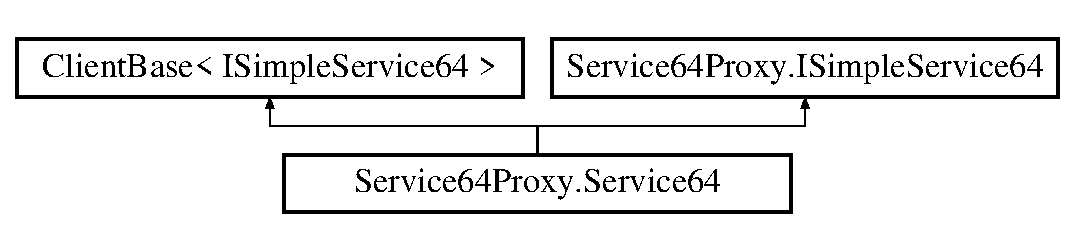
\includegraphics[height=2.000000cm]{class_service64_proxy_1_1_service64}
\end{center}
\end{figure}
\subsection*{Public Member Functions}
\begin{DoxyCompactItemize}
\item 
\mbox{\Hypertarget{class_service64_proxy_1_1_service64_a0f8d3d06960796d729fb3abea0e978a8}\label{class_service64_proxy_1_1_service64_a0f8d3d06960796d729fb3abea0e978a8}} 
\mbox{\hyperlink{class_objects_1_1_my_object}{My\+Object}} {\bfseries Load64\+Imports} (\mbox{\hyperlink{class_objects_1_1_my_object}{My\+Object}} my\+Object, string file\+Path, bool mapped\+As\+Image)
\item 
\mbox{\Hypertarget{class_service64_proxy_1_1_service64_a6cfaf78f933d791bbf393e87554d974f}\label{class_service64_proxy_1_1_service64_a6cfaf78f933d791bbf393e87554d974f}} 
\mbox{\hyperlink{class_objects_1_1_export_object}{Export\+Object}} {\bfseries Load64\+Exports} (\mbox{\hyperlink{class_objects_1_1_export_object}{Export\+Object}} my\+Object, string file\+Path, bool mapped\+As\+Image)
\end{DoxyCompactItemize}


\subsection{Detailed Description}


Definition at line 26 of file I\+P\+C\+Client.\+cs.



The documentation for this class was generated from the following file\+:\begin{DoxyCompactItemize}
\item 
C\+:/\+Users/\+Shehan Vanderputt/\+Downloads/\+Compressed/\+P\+E\+D\+Scanner-\/master/\+P\+E\+D\+Scanner-\/master/\+P\+E\+D\+Scanner\+Lib/\+P\+E\+D\+Scanner\+Lib/I\+P\+C\+Client.\+cs\end{DoxyCompactItemize}

\hypertarget{class_server64_1_1_service64}{}\section{Server64.\+Service64 Class Reference}
\label{class_server64_1_1_service64}\index{Server64.\+Service64@{Server64.\+Service64}}
Inheritance diagram for Server64.\+Service64\+:\begin{figure}[H]
\begin{center}
\leavevmode
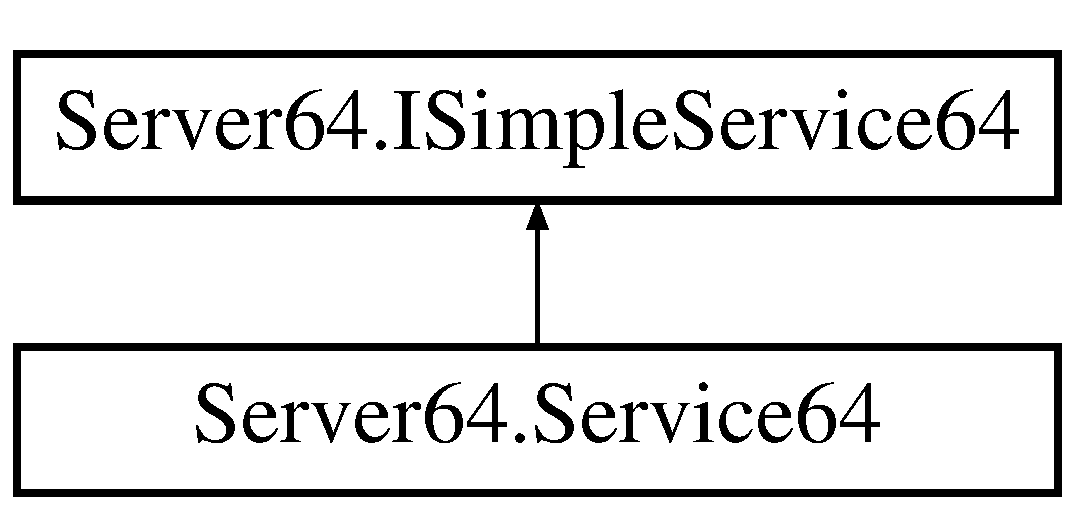
\includegraphics[height=2.000000cm]{class_server64_1_1_service64}
\end{center}
\end{figure}
\subsection*{Public Member Functions}
\begin{DoxyCompactItemize}
\item 
\mbox{\Hypertarget{class_server64_1_1_service64_a810e3a5b7c788a01feb3ac83f1a47a35}\label{class_server64_1_1_service64_a810e3a5b7c788a01feb3ac83f1a47a35}} 
\mbox{\hyperlink{class_objects_1_1_export_object}{Export\+Object}} {\bfseries Load64\+Exports} (\mbox{\hyperlink{class_objects_1_1_export_object}{Export\+Object}} my\+Object, string file\+Path, bool mapped\+As\+Image)
\item 
\mbox{\Hypertarget{class_server64_1_1_service64_ae73f54f0755da6925ff5382c3f5d2bc2}\label{class_server64_1_1_service64_ae73f54f0755da6925ff5382c3f5d2bc2}} 
\mbox{\hyperlink{class_objects_1_1_my_object}{My\+Object}} {\bfseries Load64\+Imports} (\mbox{\hyperlink{class_objects_1_1_my_object}{My\+Object}} my\+Object, string file\+Path, bool mapped\+As\+Image)
\end{DoxyCompactItemize}


\subsection{Detailed Description}


Definition at line 96 of file Class1.\+cs.



The documentation for this class was generated from the following file\+:\begin{DoxyCompactItemize}
\item 
C\+:/\+Users/\+Shehan Vanderputt/\+Downloads/\+Compressed/\+P\+E\+D\+Scanner-\/master/\+P\+E\+D\+Scanner-\/master/\+Server64\+Bit\+Library/\+Server64\+Bit\+Library/Class1.\+cs\end{DoxyCompactItemize}

\hypertarget{class_p_e_d_scanner_lib_1_1_smart_suggestion_engine}{}\section{P\+E\+D\+Scanner\+Lib.\+Smart\+Suggestion\+Engine Class Reference}
\label{class_p_e_d_scanner_lib_1_1_smart_suggestion_engine}\index{P\+E\+D\+Scanner\+Lib.\+Smart\+Suggestion\+Engine@{P\+E\+D\+Scanner\+Lib.\+Smart\+Suggestion\+Engine}}
\subsection*{Public Member Functions}
\begin{DoxyCompactItemize}
\item 
\mbox{\Hypertarget{class_p_e_d_scanner_lib_1_1_smart_suggestion_engine_a1496a35e67a3e90137658dfc4ac42bd5}\label{class_p_e_d_scanner_lib_1_1_smart_suggestion_engine_a1496a35e67a3e90137658dfc4ac42bd5}} 
void {\bfseries read\+Error\+Code} (string name, int error\+\_\+code)
\end{DoxyCompactItemize}
\subsection*{Public Attributes}
\begin{DoxyCompactItemize}
\item 
\mbox{\Hypertarget{class_p_e_d_scanner_lib_1_1_smart_suggestion_engine_ab57b34b7c0fe4a09b74ff75c2e1273ec}\label{class_p_e_d_scanner_lib_1_1_smart_suggestion_engine_ab57b34b7c0fe4a09b74ff75c2e1273ec}} 
Dictionary$<$ string, List$<$ string $>$ $>$ {\bfseries error\+\_\+list} = new Dictionary$<$string, List$<$string$>$$>$()
\end{DoxyCompactItemize}


\subsection{Detailed Description}


Definition at line 8 of file Smart\+Suggestion\+Engine.\+cs.



The documentation for this class was generated from the following file\+:\begin{DoxyCompactItemize}
\item 
C\+:/\+Users/\+Shehan Vanderputt/\+Downloads/\+Compressed/\+P\+E\+D\+Scanner-\/master/\+P\+E\+D\+Scanner-\/master/\+P\+E\+D\+Scanner\+Lib/\+P\+E\+D\+Scanner\+Lib/Smart\+Suggestion\+Engine.\+cs\end{DoxyCompactItemize}

\hypertarget{struct_class_library_server_1_1_struct_1_1_t_h_u_n_k___d_a_t_a}{}\section{Class\+Library\+Server.\+Struct.\+T\+H\+U\+N\+K\+\_\+\+D\+A\+TA Struct Reference}
\label{struct_class_library_server_1_1_struct_1_1_t_h_u_n_k___d_a_t_a}\index{Class\+Library\+Server.\+Struct.\+T\+H\+U\+N\+K\+\_\+\+D\+A\+TA@{Class\+Library\+Server.\+Struct.\+T\+H\+U\+N\+K\+\_\+\+D\+A\+TA}}
\subsection*{Public Attributes}
\begin{DoxyCompactItemize}
\item 
\mbox{\Hypertarget{struct_class_library_server_1_1_struct_1_1_t_h_u_n_k___d_a_t_a_ad3250355abd709e2cec85824004c32bd}\label{struct_class_library_server_1_1_struct_1_1_t_h_u_n_k___d_a_t_a_ad3250355abd709e2cec85824004c32bd}} 
uint {\bfseries Forwarder\+String}
\item 
\mbox{\Hypertarget{struct_class_library_server_1_1_struct_1_1_t_h_u_n_k___d_a_t_a_a4df01850945607d80f8924690e170a19}\label{struct_class_library_server_1_1_struct_1_1_t_h_u_n_k___d_a_t_a_a4df01850945607d80f8924690e170a19}} 
uint {\bfseries Function}
\item 
\mbox{\Hypertarget{struct_class_library_server_1_1_struct_1_1_t_h_u_n_k___d_a_t_a_abb64a8e37b2c6731c5413bd49a4ac595}\label{struct_class_library_server_1_1_struct_1_1_t_h_u_n_k___d_a_t_a_abb64a8e37b2c6731c5413bd49a4ac595}} 
uint {\bfseries Ordinal}
\item 
\mbox{\Hypertarget{struct_class_library_server_1_1_struct_1_1_t_h_u_n_k___d_a_t_a_aba593431b4830604ea4f7dbf2b4b7c19}\label{struct_class_library_server_1_1_struct_1_1_t_h_u_n_k___d_a_t_a_aba593431b4830604ea4f7dbf2b4b7c19}} 
uint {\bfseries Address\+Of\+Data}
\end{DoxyCompactItemize}


\subsection{Detailed Description}


Definition at line 70 of file Native\+Dll\+Structure.\+cs.



The documentation for this struct was generated from the following file\+:\begin{DoxyCompactItemize}
\item 
C\+:/\+Users/\+Shehan Vanderputt/\+Downloads/\+Compressed/\+P\+E\+D\+Scanner-\/master/\+P\+E\+D\+Scanner-\/master/\+Server64\+Bit\+Library/\+Server64\+Bit\+Library/Native\+Dll\+Structure.\+cs\end{DoxyCompactItemize}

\hypertarget{struct_p_e_d_scanner_lib_1_1_struct_1_1_t_h_u_n_k___d_a_t_a}{}\section{P\+E\+D\+Scanner\+Lib.\+Struct.\+T\+H\+U\+N\+K\+\_\+\+D\+A\+TA Struct Reference}
\label{struct_p_e_d_scanner_lib_1_1_struct_1_1_t_h_u_n_k___d_a_t_a}\index{P\+E\+D\+Scanner\+Lib.\+Struct.\+T\+H\+U\+N\+K\+\_\+\+D\+A\+TA@{P\+E\+D\+Scanner\+Lib.\+Struct.\+T\+H\+U\+N\+K\+\_\+\+D\+A\+TA}}
\subsection*{Public Attributes}
\begin{DoxyCompactItemize}
\item 
\mbox{\Hypertarget{struct_p_e_d_scanner_lib_1_1_struct_1_1_t_h_u_n_k___d_a_t_a_a603fddd7cf2ea8228fc9720cb0a93f3c}\label{struct_p_e_d_scanner_lib_1_1_struct_1_1_t_h_u_n_k___d_a_t_a_a603fddd7cf2ea8228fc9720cb0a93f3c}} 
uint {\bfseries Forwarder\+String}
\item 
\mbox{\Hypertarget{struct_p_e_d_scanner_lib_1_1_struct_1_1_t_h_u_n_k___d_a_t_a_ab1d4d3a3112911e2bdcab42e382a2017}\label{struct_p_e_d_scanner_lib_1_1_struct_1_1_t_h_u_n_k___d_a_t_a_ab1d4d3a3112911e2bdcab42e382a2017}} 
uint {\bfseries Function}
\item 
\mbox{\Hypertarget{struct_p_e_d_scanner_lib_1_1_struct_1_1_t_h_u_n_k___d_a_t_a_a99b94868eb1a8ca0642ffe7c47d66298}\label{struct_p_e_d_scanner_lib_1_1_struct_1_1_t_h_u_n_k___d_a_t_a_a99b94868eb1a8ca0642ffe7c47d66298}} 
uint {\bfseries Ordinal}
\item 
\mbox{\Hypertarget{struct_p_e_d_scanner_lib_1_1_struct_1_1_t_h_u_n_k___d_a_t_a_a81bb1d4b9aca3be04cf162e1de6c47ae}\label{struct_p_e_d_scanner_lib_1_1_struct_1_1_t_h_u_n_k___d_a_t_a_a81bb1d4b9aca3be04cf162e1de6c47ae}} 
uint {\bfseries Address\+Of\+Data}
\end{DoxyCompactItemize}


\subsection{Detailed Description}


Definition at line 41 of file Native\+Dll\+Structs.\+cs.



The documentation for this struct was generated from the following file\+:\begin{DoxyCompactItemize}
\item 
C\+:/\+Users/\+Shehan Vanderputt/\+Downloads/\+Compressed/\+P\+E\+D\+Scanner-\/master/\+P\+E\+D\+Scanner-\/master/\+P\+E\+D\+Scanner\+Lib/\+P\+E\+D\+Scanner\+Lib/Native\+Dll\+Structs.\+cs\end{DoxyCompactItemize}

\hypertarget{struct_class_library_server_1_1_struct_1_1_pe_header_reader_1_1_t_h_u_n_k___d_a_t_a}{}\section{Class\+Library\+Server.\+Struct.\+Pe\+Header\+Reader.\+T\+H\+U\+N\+K\+\_\+\+D\+A\+TA Struct Reference}
\label{struct_class_library_server_1_1_struct_1_1_pe_header_reader_1_1_t_h_u_n_k___d_a_t_a}\index{Class\+Library\+Server.\+Struct.\+Pe\+Header\+Reader.\+T\+H\+U\+N\+K\+\_\+\+D\+A\+TA@{Class\+Library\+Server.\+Struct.\+Pe\+Header\+Reader.\+T\+H\+U\+N\+K\+\_\+\+D\+A\+TA}}
\subsection*{Public Attributes}
\begin{DoxyCompactItemize}
\item 
\mbox{\Hypertarget{struct_class_library_server_1_1_struct_1_1_pe_header_reader_1_1_t_h_u_n_k___d_a_t_a_a31cf105d9ec05b865294560fdb1382d5}\label{struct_class_library_server_1_1_struct_1_1_pe_header_reader_1_1_t_h_u_n_k___d_a_t_a_a31cf105d9ec05b865294560fdb1382d5}} 
uint {\bfseries Forwarder\+String}
\item 
\mbox{\Hypertarget{struct_class_library_server_1_1_struct_1_1_pe_header_reader_1_1_t_h_u_n_k___d_a_t_a_abfe09078952795a5fc8c26d0cf8b8ade}\label{struct_class_library_server_1_1_struct_1_1_pe_header_reader_1_1_t_h_u_n_k___d_a_t_a_abfe09078952795a5fc8c26d0cf8b8ade}} 
uint {\bfseries Function}
\item 
\mbox{\Hypertarget{struct_class_library_server_1_1_struct_1_1_pe_header_reader_1_1_t_h_u_n_k___d_a_t_a_ac512dc011b05d21057659aea835b7028}\label{struct_class_library_server_1_1_struct_1_1_pe_header_reader_1_1_t_h_u_n_k___d_a_t_a_ac512dc011b05d21057659aea835b7028}} 
uint {\bfseries Ordinal}
\item 
\mbox{\Hypertarget{struct_class_library_server_1_1_struct_1_1_pe_header_reader_1_1_t_h_u_n_k___d_a_t_a_a06558fc4f7b01d40b801fe585afe7ada}\label{struct_class_library_server_1_1_struct_1_1_pe_header_reader_1_1_t_h_u_n_k___d_a_t_a_a06558fc4f7b01d40b801fe585afe7ada}} 
uint {\bfseries Address\+Of\+Data}
\end{DoxyCompactItemize}


\subsection{Detailed Description}


Definition at line 588 of file Native\+Dll\+Structure.\+cs.



The documentation for this struct was generated from the following file\+:\begin{DoxyCompactItemize}
\item 
C\+:/\+Users/\+Shehan Vanderputt/\+Downloads/\+Compressed/\+P\+E\+D\+Scanner-\/master/\+P\+E\+D\+Scanner-\/master/\+Server64\+Bit\+Library/\+Server64\+Bit\+Library/Native\+Dll\+Structure.\+cs\end{DoxyCompactItemize}

\hypertarget{struct_p_e_d_scanner_lib_1_1_struct_1_1_pe_header_reader_1_1_t_h_u_n_k___d_a_t_a}{}\section{P\+E\+D\+Scanner\+Lib.\+Struct.\+Pe\+Header\+Reader.\+T\+H\+U\+N\+K\+\_\+\+D\+A\+TA Struct Reference}
\label{struct_p_e_d_scanner_lib_1_1_struct_1_1_pe_header_reader_1_1_t_h_u_n_k___d_a_t_a}\index{P\+E\+D\+Scanner\+Lib.\+Struct.\+Pe\+Header\+Reader.\+T\+H\+U\+N\+K\+\_\+\+D\+A\+TA@{P\+E\+D\+Scanner\+Lib.\+Struct.\+Pe\+Header\+Reader.\+T\+H\+U\+N\+K\+\_\+\+D\+A\+TA}}
\subsection*{Public Attributes}
\begin{DoxyCompactItemize}
\item 
\mbox{\Hypertarget{struct_p_e_d_scanner_lib_1_1_struct_1_1_pe_header_reader_1_1_t_h_u_n_k___d_a_t_a_af0902812d8d93dff6f3c46e78db5de47}\label{struct_p_e_d_scanner_lib_1_1_struct_1_1_pe_header_reader_1_1_t_h_u_n_k___d_a_t_a_af0902812d8d93dff6f3c46e78db5de47}} 
uint {\bfseries Forwarder\+String}
\item 
\mbox{\Hypertarget{struct_p_e_d_scanner_lib_1_1_struct_1_1_pe_header_reader_1_1_t_h_u_n_k___d_a_t_a_a1587508523e3370dd1a0ee399a8d7ca8}\label{struct_p_e_d_scanner_lib_1_1_struct_1_1_pe_header_reader_1_1_t_h_u_n_k___d_a_t_a_a1587508523e3370dd1a0ee399a8d7ca8}} 
uint {\bfseries Function}
\item 
\mbox{\Hypertarget{struct_p_e_d_scanner_lib_1_1_struct_1_1_pe_header_reader_1_1_t_h_u_n_k___d_a_t_a_a6257aaca8da11e253ae11e065bc60736}\label{struct_p_e_d_scanner_lib_1_1_struct_1_1_pe_header_reader_1_1_t_h_u_n_k___d_a_t_a_a6257aaca8da11e253ae11e065bc60736}} 
uint {\bfseries Ordinal}
\item 
\mbox{\Hypertarget{struct_p_e_d_scanner_lib_1_1_struct_1_1_pe_header_reader_1_1_t_h_u_n_k___d_a_t_a_a17d9d3b537f1c268e7e7157208e9406d}\label{struct_p_e_d_scanner_lib_1_1_struct_1_1_pe_header_reader_1_1_t_h_u_n_k___d_a_t_a_a17d9d3b537f1c268e7e7157208e9406d}} 
uint {\bfseries Address\+Of\+Data}
\end{DoxyCompactItemize}


\subsection{Detailed Description}


Definition at line 568 of file Native\+Dll\+Structs.\+cs.



The documentation for this struct was generated from the following file\+:\begin{DoxyCompactItemize}
\item 
C\+:/\+Users/\+Shehan Vanderputt/\+Downloads/\+Compressed/\+P\+E\+D\+Scanner-\/master/\+P\+E\+D\+Scanner-\/master/\+P\+E\+D\+Scanner\+Lib/\+P\+E\+D\+Scanner\+Lib/Native\+Dll\+Structs.\+cs\end{DoxyCompactItemize}

\hypertarget{struct_class_library_server_1_1_struct_1_1_t_h_u_n_k___d_a_t_a64}{}\section{Class\+Library\+Server.\+Struct.\+T\+H\+U\+N\+K\+\_\+\+D\+A\+T\+A64 Struct Reference}
\label{struct_class_library_server_1_1_struct_1_1_t_h_u_n_k___d_a_t_a64}\index{Class\+Library\+Server.\+Struct.\+T\+H\+U\+N\+K\+\_\+\+D\+A\+T\+A64@{Class\+Library\+Server.\+Struct.\+T\+H\+U\+N\+K\+\_\+\+D\+A\+T\+A64}}
\subsection*{Public Attributes}
\begin{DoxyCompactItemize}
\item 
\mbox{\Hypertarget{struct_class_library_server_1_1_struct_1_1_t_h_u_n_k___d_a_t_a64_a3c1a35933a1fb6204aa82f38f92600e3}\label{struct_class_library_server_1_1_struct_1_1_t_h_u_n_k___d_a_t_a64_a3c1a35933a1fb6204aa82f38f92600e3}} 
ulong {\bfseries Forwarder\+String}
\item 
\mbox{\Hypertarget{struct_class_library_server_1_1_struct_1_1_t_h_u_n_k___d_a_t_a64_ab2784b529fec7927b230d3baada26493}\label{struct_class_library_server_1_1_struct_1_1_t_h_u_n_k___d_a_t_a64_ab2784b529fec7927b230d3baada26493}} 
ulong {\bfseries Function}
\item 
\mbox{\Hypertarget{struct_class_library_server_1_1_struct_1_1_t_h_u_n_k___d_a_t_a64_a4e632fcf0f42805dcc99222258780847}\label{struct_class_library_server_1_1_struct_1_1_t_h_u_n_k___d_a_t_a64_a4e632fcf0f42805dcc99222258780847}} 
ulong {\bfseries Ordinal}
\item 
\mbox{\Hypertarget{struct_class_library_server_1_1_struct_1_1_t_h_u_n_k___d_a_t_a64_a22e5cc24319658541dd23702a97cffcf}\label{struct_class_library_server_1_1_struct_1_1_t_h_u_n_k___d_a_t_a64_a22e5cc24319658541dd23702a97cffcf}} 
ulong {\bfseries Address\+Of\+Data}
\end{DoxyCompactItemize}


\subsection{Detailed Description}


Definition at line 82 of file Native\+Dll\+Structure.\+cs.



The documentation for this struct was generated from the following file\+:\begin{DoxyCompactItemize}
\item 
C\+:/\+Users/\+Shehan Vanderputt/\+Downloads/\+Compressed/\+P\+E\+D\+Scanner-\/master/\+P\+E\+D\+Scanner-\/master/\+Server64\+Bit\+Library/\+Server64\+Bit\+Library/Native\+Dll\+Structure.\+cs\end{DoxyCompactItemize}

\hypertarget{class_wizard_1_1_welcome_page_function}{}\section{Wizard.\+Welcome\+Page\+Function Class Reference}
\label{class_wizard_1_1_welcome_page_function}\index{Wizard.\+Welcome\+Page\+Function@{Wizard.\+Welcome\+Page\+Function}}


Interaction logic for Welcome\+Page\+Function.\+xaml  


Inheritance diagram for Wizard.\+Welcome\+Page\+Function\+:\begin{figure}[H]
\begin{center}
\leavevmode
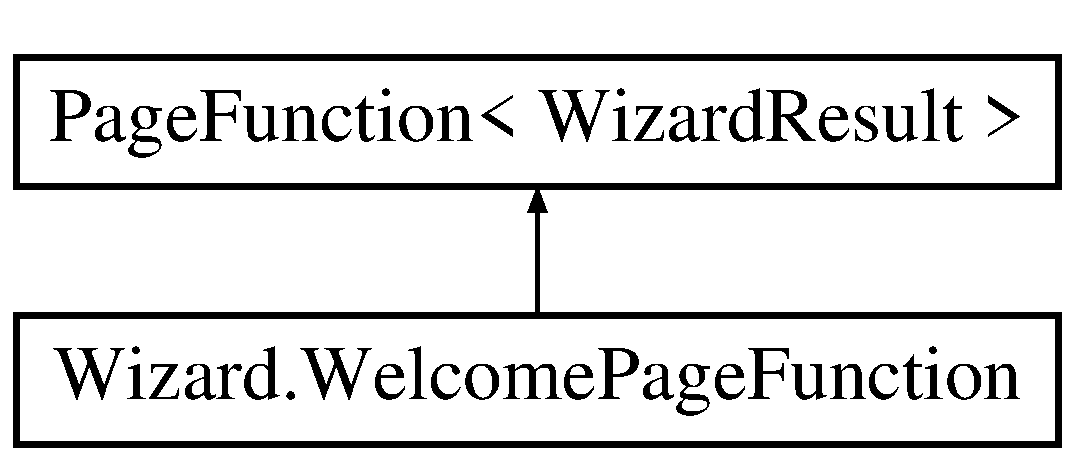
\includegraphics[height=2.000000cm]{class_wizard_1_1_welcome_page_function}
\end{center}
\end{figure}
\subsection*{Public Member Functions}
\begin{DoxyCompactItemize}
\item 
\mbox{\Hypertarget{class_wizard_1_1_welcome_page_function_a76a28a62c6b572604a83ea819123cfdb}\label{class_wizard_1_1_welcome_page_function_a76a28a62c6b572604a83ea819123cfdb}} 
{\bfseries Welcome\+Page\+Function} (\mbox{\hyperlink{class_wizard_1_1_wizard_data}{Wizard\+Data}} wizard\+Data)
\item 
\mbox{\Hypertarget{class_wizard_1_1_welcome_page_function_a4b4237e738fc47d3d41cb68e58f82623}\label{class_wizard_1_1_welcome_page_function_a4b4237e738fc47d3d41cb68e58f82623}} 
void {\bfseries wizard\+Page\+\_\+\+Return} (object sender, Return\+Event\+Args$<$ Wizard\+Result $>$ e)
\end{DoxyCompactItemize}


\subsection{Detailed Description}
Interaction logic for Welcome\+Page\+Function.\+xaml 

Definition at line 24 of file Welcome\+Page\+Function.\+xaml.\+cs.



The documentation for this class was generated from the following file\+:\begin{DoxyCompactItemize}
\item 
C\+:/\+Users/\+Shehan Vanderputt/\+Downloads/\+Compressed/\+P\+E\+D\+Scanner-\/master/\+P\+E\+D\+Scanner-\/master/\+P\+E\+D\+Scanner\+G\+U\+I\+W\+P\+F/\+P\+E\+D\+Scanner/\+P\+E\+D\+Scanner/Welcome\+Page\+Function.\+xaml.\+cs\end{DoxyCompactItemize}

\hypertarget{class_wizard_1_1_wizard_data}{}\section{Wizard.\+Wizard\+Data Class Reference}
\label{class_wizard_1_1_wizard_data}\index{Wizard.\+Wizard\+Data@{Wizard.\+Wizard\+Data}}


Data that is collected by the wizard  


\subsection*{Properties}
\begin{DoxyCompactItemize}
\item 
\mbox{\Hypertarget{class_wizard_1_1_wizard_data_a3e0ea7eb20774a38417dc869ec5d47ce}\label{class_wizard_1_1_wizard_data_a3e0ea7eb20774a38417dc869ec5d47ce}} 
string {\bfseries Data\+Item1}\hspace{0.3cm}{\ttfamily  \mbox{[}get, set\mbox{]}}
\item 
\mbox{\Hypertarget{class_wizard_1_1_wizard_data_ab17f76526a0d20dafeee21d665a9fff3}\label{class_wizard_1_1_wizard_data_ab17f76526a0d20dafeee21d665a9fff3}} 
string {\bfseries Data\+Item2}\hspace{0.3cm}{\ttfamily  \mbox{[}get, set\mbox{]}}
\item 
\mbox{\Hypertarget{class_wizard_1_1_wizard_data_ae011153e97a4632b878e0cac4bcb14e4}\label{class_wizard_1_1_wizard_data_ae011153e97a4632b878e0cac4bcb14e4}} 
string {\bfseries Data\+Item3}\hspace{0.3cm}{\ttfamily  \mbox{[}get, set\mbox{]}}
\item 
\mbox{\Hypertarget{class_wizard_1_1_wizard_data_afbc437376df3470d60c79ec957c36f58}\label{class_wizard_1_1_wizard_data_afbc437376df3470d60c79ec957c36f58}} 
string {\bfseries Folder\+Path}\hspace{0.3cm}{\ttfamily  \mbox{[}get, set\mbox{]}}
\item 
\mbox{\Hypertarget{class_wizard_1_1_wizard_data_a469073e0e30443a5dba2170507fc867c}\label{class_wizard_1_1_wizard_data_a469073e0e30443a5dba2170507fc867c}} 
string {\bfseries File\+Path}\hspace{0.3cm}{\ttfamily  \mbox{[}get, set\mbox{]}}
\end{DoxyCompactItemize}


\subsection{Detailed Description}
Data that is collected by the wizard 



Definition at line 9 of file Wizard\+Data.\+cs.



The documentation for this class was generated from the following file\+:\begin{DoxyCompactItemize}
\item 
C\+:/\+Users/\+Shehan Vanderputt/\+Downloads/\+Compressed/\+P\+E\+D\+Scanner-\/master/\+P\+E\+D\+Scanner-\/master/\+P\+E\+D\+Scanner\+G\+U\+I\+W\+P\+F/\+P\+E\+D\+Scanner/\+P\+E\+D\+Scanner/Wizard\+Data.\+cs\end{DoxyCompactItemize}

\hypertarget{class_wizard_1_1_wizard_dialog_box}{}\section{Wizard.\+Wizard\+Dialog\+Box Class Reference}
\label{class_wizard_1_1_wizard_dialog_box}\index{Wizard.\+Wizard\+Dialog\+Box@{Wizard.\+Wizard\+Dialog\+Box}}
Inheritance diagram for Wizard.\+Wizard\+Dialog\+Box\+:\begin{figure}[H]
\begin{center}
\leavevmode
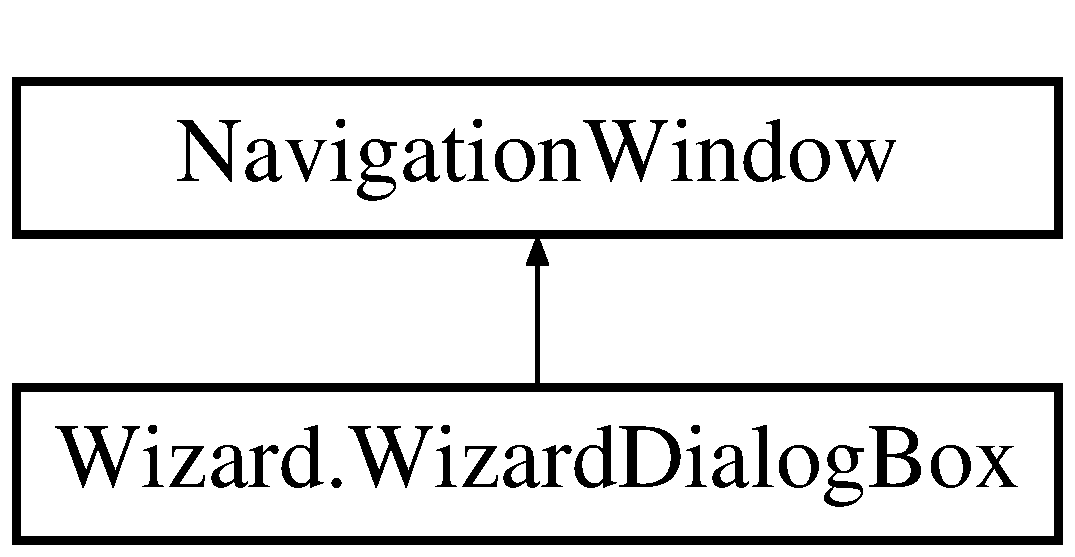
\includegraphics[height=2.000000cm]{class_wizard_1_1_wizard_dialog_box}
\end{center}
\end{figure}
\subsection*{Properties}
\begin{DoxyCompactItemize}
\item 
\mbox{\Hypertarget{class_wizard_1_1_wizard_dialog_box_a3fd28ae9e2a049e9ac0966bf1c829879}\label{class_wizard_1_1_wizard_dialog_box_a3fd28ae9e2a049e9ac0966bf1c829879}} 
\mbox{\hyperlink{class_wizard_1_1_wizard_data}{Wizard\+Data}} {\bfseries Wizard\+Data}\hspace{0.3cm}{\ttfamily  \mbox{[}get\mbox{]}}
\end{DoxyCompactItemize}


\subsection{Detailed Description}


Definition at line 6 of file Wizard\+Dialog\+Box.\+xaml.\+cs.



The documentation for this class was generated from the following file\+:\begin{DoxyCompactItemize}
\item 
C\+:/\+Users/\+Shehan Vanderputt/\+Downloads/\+Compressed/\+P\+E\+D\+Scanner-\/master/\+P\+E\+D\+Scanner-\/master/\+P\+E\+D\+Scanner\+G\+U\+I\+W\+P\+F/\+P\+E\+D\+Scanner/\+P\+E\+D\+Scanner/Wizard\+Dialog\+Box.\+xaml.\+cs\end{DoxyCompactItemize}

\hypertarget{class_wizard_1_1_wizard_launcher}{}\section{Wizard.\+Wizard\+Launcher Class Reference}
\label{class_wizard_1_1_wizard_launcher}\index{Wizard.\+Wizard\+Launcher@{Wizard.\+Wizard\+Launcher}}
Inheritance diagram for Wizard.\+Wizard\+Launcher\+:\begin{figure}[H]
\begin{center}
\leavevmode
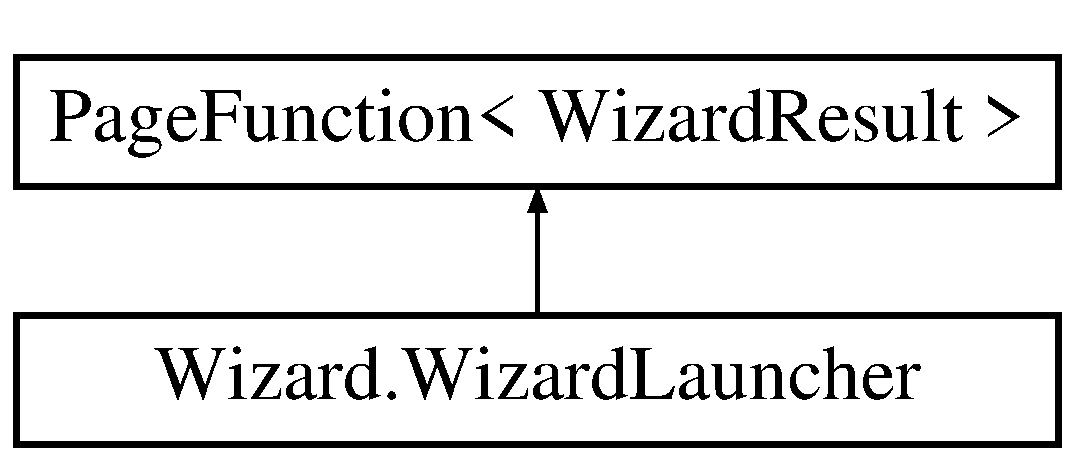
\includegraphics[height=2.000000cm]{class_wizard_1_1_wizard_launcher}
\end{center}
\end{figure}
\subsection*{Public Member Functions}
\begin{DoxyCompactItemize}
\item 
\mbox{\Hypertarget{class_wizard_1_1_wizard_launcher_a78bed6b60e2bac289fa3815982f3b30f}\label{class_wizard_1_1_wizard_launcher_a78bed6b60e2bac289fa3815982f3b30f}} 
void {\bfseries wizard\+Page\+\_\+\+Return} (object sender, Return\+Event\+Args$<$ Wizard\+Result $>$ e)
\end{DoxyCompactItemize}
\subsection*{Protected Member Functions}
\begin{DoxyCompactItemize}
\item 
\mbox{\Hypertarget{class_wizard_1_1_wizard_launcher_a9e6920c61becaa61c5482daac33339c5}\label{class_wizard_1_1_wizard_launcher_a9e6920c61becaa61c5482daac33339c5}} 
override void {\bfseries Start} ()
\end{DoxyCompactItemize}
\subsection*{Events}
\begin{DoxyCompactItemize}
\item 
\mbox{\Hypertarget{class_wizard_1_1_wizard_launcher_a17588d6769064bbe93a042dbcd12deff}\label{class_wizard_1_1_wizard_launcher_a17588d6769064bbe93a042dbcd12deff}} 
Wizard\+Return\+Event\+Handler {\bfseries Wizard\+Return}
\end{DoxyCompactItemize}


\subsection{Detailed Description}


Definition at line 8 of file Wizard\+Launcher.\+cs.



The documentation for this class was generated from the following file\+:\begin{DoxyCompactItemize}
\item 
C\+:/\+Users/\+Shehan Vanderputt/\+Downloads/\+Compressed/\+P\+E\+D\+Scanner-\/master/\+P\+E\+D\+Scanner-\/master/\+P\+E\+D\+Scanner\+G\+U\+I\+W\+P\+F/\+P\+E\+D\+Scanner/\+P\+E\+D\+Scanner/Wizard\+Launcher.\+cs\end{DoxyCompactItemize}

\hypertarget{class_wizard_1_1_wizard_return_event_args}{}\section{Wizard.\+Wizard\+Return\+Event\+Args Class Reference}
\label{class_wizard_1_1_wizard_return_event_args}\index{Wizard.\+Wizard\+Return\+Event\+Args@{Wizard.\+Wizard\+Return\+Event\+Args}}
\subsection*{Public Member Functions}
\begin{DoxyCompactItemize}
\item 
\mbox{\Hypertarget{class_wizard_1_1_wizard_return_event_args_a173874e1e44724f14afc19ed6c9db718}\label{class_wizard_1_1_wizard_return_event_args_a173874e1e44724f14afc19ed6c9db718}} 
{\bfseries Wizard\+Return\+Event\+Args} (Wizard\+Result result, object data)
\end{DoxyCompactItemize}
\subsection*{Properties}
\begin{DoxyCompactItemize}
\item 
\mbox{\Hypertarget{class_wizard_1_1_wizard_return_event_args_ac8ce7f3ad4a2cd81714c8b29e772dc41}\label{class_wizard_1_1_wizard_return_event_args_ac8ce7f3ad4a2cd81714c8b29e772dc41}} 
Wizard\+Result {\bfseries Result}\hspace{0.3cm}{\ttfamily  \mbox{[}get\mbox{]}}
\item 
\mbox{\Hypertarget{class_wizard_1_1_wizard_return_event_args_aaa15c75ee0435fceb69e6f4196b0f51a}\label{class_wizard_1_1_wizard_return_event_args_aaa15c75ee0435fceb69e6f4196b0f51a}} 
object {\bfseries Data}\hspace{0.3cm}{\ttfamily  \mbox{[}get\mbox{]}}
\end{DoxyCompactItemize}


\subsection{Detailed Description}


Definition at line 6 of file Wizard\+Return\+Event\+Args.\+cs.



The documentation for this class was generated from the following file\+:\begin{DoxyCompactItemize}
\item 
C\+:/\+Users/\+Shehan Vanderputt/\+Downloads/\+Compressed/\+P\+E\+D\+Scanner-\/master/\+P\+E\+D\+Scanner-\/master/\+P\+E\+D\+Scanner\+G\+U\+I\+W\+P\+F/\+P\+E\+D\+Scanner/\+P\+E\+D\+Scanner/Wizard\+Return\+Event\+Args.\+cs\end{DoxyCompactItemize}

%--- End generated contents ---

% Index
\backmatter
\newpage
\phantomsection
\clearemptydoublepage
\addcontentsline{toc}{chapter}{Index}
\printindex

\end{document}
